\documentclass{article}
\usepackage[a4paper, margin=1in]{geometry}

\usepackage{url}


\usepackage{graphicx}
\usepackage[english]{babel}
\usepackage[utf8]{inputenc}
%\usepackage{hyperref}
\usepackage{xcolor}
\usepackage{subcaption}
%\captionsetup{compatibility=false}
\usepackage{amsmath}

%\usepackage[dvipsnames]{xcolor}

\usepackage{authblk} %this line causes problems with some journal formats
%\usepackage{lineno}
%\linenumbers
%\pgfplotsset{compat=newest}


%%%%% this block calls the tikz library and externalizes the figure compiling to save calculation time
%%%%% sometimes you have to delete the files to force recreation of the images if you made changes to the formatting and the images don't change
\usepackage{pgfplots}
\usepackage{tikz}
\usetikzlibrary{external}
\tikzexternalize
\tikzsetexternalprefix{./tikz_compiled/}
\tikzset{external/system call={lualatex \tikzexternalcheckshellescape 
		-interaction=batchmode -jobname "\image" "\texsource"}} % or ;
%	pdftops -eps "\image".pdf}} #this line might convert your pdf-images to eps for paper submission, but always involves tweaking

%%%%%%%% check the embedded image tex-file for more comments

\bibliographystyle{./embedded_files/spphys}

\newcommand{\rulesep}{\unskip\ \vrule\ }

\begin{document}

	
\title{Title}
\author[1]{Robert Fischer}
\author[2]{Somebody Else}

\affil[1]{Electrochemistry Laboratory, Paul Scherrer Institut, Forschungsstrasse 111, 5242 Villigen PSI, Switzerland}
\affil[2]{lab, institute, street, city, country} 

\date{\today}
\maketitle

\begin{abstract}
		
\textit{Hypothesis}\\


\textit{Experiments}\\


\textit{Findings}\\


\end{abstract}
%\maketitle

\section{Introduction}




\section{Methods}

 

\section{Results}

\begin{figure}
	\centering
	% This file was created with tikzplotlib v0.10.1.
\begin{tikzpicture}

\definecolor{darkgray176}{RGB}{176,176,176}

\begin{axis}[
width=\textwidth,
height=0.3\textheight,
ylabel near ticks,
tick align=outside,
tick pos=left,
legend style={nodes={scale=0.8, transform shape}, fill opacity=0.8, draw opacity=1, text opacity=1, draw=white!80!black, legend pos=north west},
x grid style={darkgray176},
xlabel={time [min]},
xmin=0, xmax=68,
xtick style={color=black},
y grid style={darkgray176},
ylabel={passed charge [\(\displaystyle As/cm^{2}\)]},
ymin=0, ymax=600,
ytick style={color=black},
axis line style = {-},
]
\addplot [semithick, black]
table {%
-11.5 -39.1668728390326
-11.4966666658719 -39.1604702884026
-11.4933166662852 -39.1543898405634
-11.4899666666985 -39.1486900608527
-11.4866333325704 -39.1434115334489
-11.4832833329837 -39.1383983639219
-11.4799499988556 -39.1336102735244
-11.4765999992688 -39.1288908448807
-11.4732499957085 -39.1242690006044
-11.4698999961217 -39.1201776933316
-11.4665666619937 -39.1155859778398
-11.4632166624069 -39.1112718137954
-11.4598833282789 -39.1072400455473
-11.4565333286921 -39.1032211095171
-11.4531999945641 -39.0989668721792
-11.4498499949773 -39.0949654267623
-11.4465166608493 -39.0908809672589
-11.4431666612625 -39.0866719255008
-11.4398166616758 -39.0824498012137
-11.4364833275477 -39.0783541419624
-11.433133327961 -39.0742334406693
-11.4297999938329 -39.0701453806494
-11.4264499942462 -39.0661787551241
-11.4231166601181 -39.06222139046
-11.4197666605314 -39.0581682327919
-11.4164333264033 -39.0541318391324
-11.4130833268166 -39.050089028886
-11.4097499926885 -39.0460163207764
-11.4063999931018 -39.0421637021268
-11.4030666589737 -39.0379953178912
-11.399716659387 -39.034067356569
-11.3963833252589 -39.0299562063009
-11.3930333256721 -39.025809286536
-11.3896999915441 -39.0216704096136
-11.3863499919573 -39.017596999757
-11.3830166578293 -39.0134165510185
-11.3796666582425 -39.0092994698988
-11.3763333280881 -39.0053101377438
-11.3729833245277 -39.0013580317279
-11.369633324941 -38.9973449372155
-11.3662999908129 -38.9933239203238
-11.3629499912262 -38.9893316212801
-11.3596166570981 -38.9851953175894
-11.3562666575114 -38.9809964193108
-11.3529333233833 -38.9768649370234
-11.3495833237966 -38.9727629854727
-11.3462499896685 -38.9686463957094
-11.3428999900818 -38.9644946468927
-11.3395666559537 -38.9601839299175
-11.336216656367 -38.9562967179622
-11.3328833222389 -38.9519706414282
-11.3295333226522 -38.9478183553066
-11.3261999885241 -38.9439060092888
-11.3228499889374 -38.9398499131747
-11.3195166548093 -38.9356303028436
-11.3161666552226 -38.9316234370448
-11.3128333250682 -38.9274977623351
-11.3094833215078 -38.9232363669868
-11.3061499913534 -38.9189048327925
-11.302799987793 -38.9146902432029
-11.2994666576386 -38.910451255477
-11.2961166540782 -38.9061944625945
-11.2927833239237 -38.9020466197551
-11.2894333203634 -38.8979480493054
-11.2860999902089 -38.8937490845808
-11.2827499866486 -38.8895304957983
-11.2794166564941 -38.8853281514067
-11.2760666529338 -38.8810515322599
-11.2727333227793 -38.8769336652024
-11.269383319219 -38.8727828910874
-11.2660499890645 -38.8683721933325
-11.2626999855042 -38.8641951582011
-11.2593666553497 -38.8599657621326
-11.2560166517893 -38.8556251406018
-11.2526833216349 -38.8511441962405
-11.2493333220482 -38.8469222153622
-11.2459999879201 -38.8425080356421
-11.2426499883334 -38.838268930799
-11.2393166542053 -38.8340806304296
-11.2359666546186 -38.8299056089897
-11.2326166510582 -38.825631161534
-11.2292666514715 -38.821417855453
-11.2259333173434 -38.817119907676
-11.222599987189 -38.8127178024974
-11.2192499836286 -38.8083259610924
-11.2158999840418 -38.8040180816989
-11.2125666499138 -38.7996882340043
-11.2092333197594 -38.7953454699462
-11.205883316199 -38.7908427026453
-11.2025333166122 -38.7865924788412
-11.1991999824842 -38.7822418048143
-11.1958666523298 -38.7779397138774
-11.1925166487694 -38.7735845511328
-11.1891666491826 -38.7693180936009
-11.1858333190282 -38.7650303224788
-11.1824999849002 -38.7607134699978
-11.1791499853134 -38.7563824945243
-11.175799981753 -38.7519492629473
-11.1724666515986 -38.7474518437679
-11.1691333174705 -38.7429684774362
-11.1657833178838 -38.7385178858629
-11.1624333143234 -38.7340341146405
-11.159099984169 -38.7296482838992
-11.1557666500409 -38.7253429982927
-11.1524166504542 -38.7209503800695
-11.1490666468938 -38.7165137262809
-11.1457333167394 -38.7121167389846
-11.1423999826113 -38.7076537405245
-11.1390499830246 -38.7032249990586
-11.1356999794642 -38.6990403154587
-11.1323666493098 -38.6941709372029
-11.1290333151817 -38.6900688933925
-11.125683315595 -38.6856404785068
-11.1223333160083 -38.6809424818094
-11.1189999818802 -38.6763072229834
-11.1156666477521 -38.6719852192589
-11.1123166481654 -38.667302740896
-11.1089666485786 -38.6628107078935
-11.1056333144506 -38.6584288256118
-11.1022999803225 -38.6540989731246
-11.0989499807358 -38.6496145962149
-11.095599981149 -38.6451860235112
-11.092266647021 -38.6407527958689
-11.0889333128929 -38.6361769308719
-11.0855833133062 -38.6315581616243
-11.0822333137194 -38.6270389550475
-11.0788999795914 -38.6225222823131
-11.0755666454633 -38.618001797008
-11.0722166458766 -38.6133971983338
-11.0688666462898 -38.6087318586846
-11.0655333121618 -38.6045482195913
-11.0621999780337 -38.5997288359632
-11.058849978447 -38.5951125989209
-11.0554999788602 -38.5907822363764
-11.0521666447322 -38.5864139749514
-11.0488333106041 -38.5817278066105
-11.0454833110174 -38.577296000755
-11.0421333114306 -38.572760366702
-11.0387999773026 -38.568096385106
-11.0354666431745 -38.563368466166
-11.0321166435877 -38.5587548734667
-11.028766644001 -38.5541162331869
-11.0254333098729 -38.5494920117131
-11.0220999757449 -38.5449736349951
-11.0187499761581 -38.5404619271371
-11.0153999765714 -38.5358609584326
-11.0120666424433 -38.5312761246712
-11.0087333083153 -38.5266754045418
-11.0053833087285 -38.5220120830498
-11.0020333091418 -38.5175878766656
-10.9986999750137 -38.5129014865788
-10.9953666408857 -38.5083718073366
-10.9920166412989 -38.5036551015519
-10.9886666417122 -38.4989870820706
-10.9853333075841 -38.4943163060204
-10.9819999734561 -38.4895985963516
-10.9786499738693 -38.4848779606657
-10.9753166397413 -38.4801830571263
-10.9719833056132 -38.4756338936538
-10.9686499714851 -38.4711025986726
-10.9652999718984 -38.4665206940016
-10.9619499723117 -38.4619025002988
-10.9585999727249 -38.4573422773758
-10.9552666385969 -38.4526965748598
-10.9519333044688 -38.4479819745523
-10.9485999743144 -38.4433017465622
-10.9452666401863 -38.4386436453235
-10.9419333060582 -38.4339309434895
-10.9385833064715 -38.4292688434447
-10.9352499723434 -38.4245303097718
-10.9319166382154 -38.4199050368719
-10.9285833040873 -38.4152011258764
-10.9252499699593 -38.4105406735986
-10.9218999703725 -38.4059324917868
-10.9185499707858 -38.401302575373
-10.915199971199 -38.3965800743653
-10.9118499716123 -38.3919694705026
-10.9085166374842 -38.3873044985156
-10.9051833033562 -38.3825223800086
-10.9018499692281 -38.3776793865482
-10.8985166351 -38.3728901622653
-10.8951666355133 -38.3680984109067
-10.8918166359266 -38.3632831398465
-10.8884666363398 -38.358559460913
-10.8851166367531 -38.3539231921363
-10.881783302625 -38.349220435087
-10.878449968497 -38.3444818918774
-10.8751166343689 -38.3397667666229
-10.8717833002408 -38.3349750317303
-10.8684333006541 -38.3302681207495
-10.8650833010674 -38.3256823013198
-10.8617333014806 -38.320573999664
-10.8583999673525 -38.3160924102319
-10.8550666332245 -38.3113844179314
-10.8517333030701 -38.3064869029554
-10.848399968942 -38.3014902172129
-10.8450666348139 -38.2968528245894
-10.8417166352272 -38.2919235903112
-10.8383833010991 -38.2871648787922
-10.8350499669711 -38.2824956243297
-10.831716632843 -38.2778880883458
-10.828383298715 -38.2731327071017
-10.8250332991282 -38.2684183087675
-10.8216832995415 -38.263663592109
-10.8183332999547 -38.258789552705
-10.814983300368 -38.2539102877833
-10.8116499662399 -38.2491321112901
-10.8083166321119 -38.2443335738454
-10.8049832979838 -38.2395449097932
-10.8016499638557 -38.2346518704579
-10.798299964269 -38.2297790501929
-10.7949499646823 -38.2251874360194
-10.7915999650955 -38.2201977624363
-10.7882499655088 -38.215314046106
-10.7849166313807 -38.2106606469596
-10.7815832972527 -38.2060368513015
-10.7782499631246 -38.2011486555751
-10.7749166289965 -38.196430727447
-10.7715666294098 -38.1915947842183
-10.768216629823 -38.1866458487574
-10.7648666302363 -38.1816752271823
-10.7615332961082 -38.1768183458363
-10.7581999619802 -38.1719314743388
-10.7548666318258 -38.1670796474988
-10.7515332976977 -38.1623294384652
-10.7481999635696 -38.1575558094096
-10.7448499639829 -38.1526960930172
-10.7415166298548 -38.1478690054176
-10.7381832957268 -38.1430244035851
-10.7348499615987 -38.1381470439857
-10.7315166274707 -38.1334970629392
-10.7281666278839 -38.1284534908589
-10.7248166282972 -38.1237903672854
-10.7214666287104 -38.1188633020462
-10.7181166291237 -38.1138501205684
-10.7147832949956 -38.1089030173191
-10.7114499608676 -38.1040707073977
-10.7081166267395 -38.0990580061217
-10.7047832926114 -38.0941434334795
-10.7014332930247 -38.0893387575228
-10.698083293438 -38.0845959341781
-10.6947332938512 -38.0797534145957
-10.6913832942645 -38.0749212169148
-10.6880499601364 -38.0701343929777
-10.6847166260084 -38.065210351963
-10.6813832918803 -38.0602353561174
-10.6780499577522 -38.0553119662252
-10.6746999581655 -38.0504027572504
-10.6713499585787 -38.0454806121762
-10.667999958992 -38.0405509151656
-10.6646666248639 -38.035484483389
-10.6613332907359 -38.0308350843407
-10.6579999605815 -38.0257145717791
-10.6546666264534 -38.0207917319175
-10.6513332923253 -38.0161010404636
-10.6479832927386 -38.0112796065679
-10.6446499586105 -38.0063229675268
-10.6413166244825 -38.001572094259
-10.6379832903544 -37.9967166000326
-10.6346499562263 -37.9917186093692
-10.6312999566396 -37.9866481199086
-10.6279499570529 -37.9816905872179
-10.6245999574661 -37.9767173111495
-10.6212499578794 -37.9717365620461
-10.6179166237513 -37.966886508533
-10.6145832896233 -37.9620879710883
-10.6112499554952 -37.9571992808816
-10.6079166213671 -37.9522726662038
-10.6045666217804 -37.9473631169819
-10.6012166221937 -37.9423815609282
-10.5978666226069 -37.9375425367858
-10.5945166230202 -37.9327322404943
-10.5911832888921 -37.9275876145577
-10.587849954764 -37.9228306029636
-10.584516620636 -37.9179461904641
-10.5811832865079 -37.9129224588801
-10.5778332869212 -37.9077564582213
-10.5744832873344 -37.9028909834602
-10.5711332877477 -37.8978317926204
-10.5677999536196 -37.8929567285156
-10.5644666194916 -37.8881355823211
-10.5611332893372 -37.8833416997581
-10.5577999552091 -37.8784414958387
-10.554466621081 -37.873587718004
-10.5511166214943 -37.8686580511093
-10.5477832873662 -37.8636474712823
-10.5444499532382 -37.858649009321
-10.5411166191101 -37.8537269962952
-10.537783284982 -37.8487708695239
-10.5344332853953 -37.8438126165635
-10.5310832858086 -37.8387264000188
-10.5277332862218 -37.8337763431801
-10.5243832866351 -37.8289541654709
-10.521049952507 -37.8239869640074
-10.517716618379 -37.8189923095917
-10.5143832842509 -37.8141940091351
-10.5110499501228 -37.8093970766301
-10.5076999505361 -37.804393467292
-10.5043499509494 -37.799528545073
-10.5009999513626 -37.7945443748672
-10.4976499517759 -37.7894805437971
-10.4943166176478 -37.7844235967907
-10.4909832835197 -37.7794513341764
-10.4876499493917 -37.7744483608576
-10.4843166152636 -37.7694875995924
-10.4809666156769 -37.7646142114502
-10.4776166160901 -37.7597032777579
-10.4742666165034 -37.7547297832269
-10.4709332823753 -37.7497981128158
-10.4675999482473 -37.7448367045446
-10.4642666180929 -37.7398792931209
-10.4609332839648 -37.7351837687394
-10.4575999498367 -37.7299224752472
-10.45424995025 -37.7252224856458
-10.4509166161219 -37.7202645558062
-10.4475832819939 -37.7150763378829
-10.4442499478658 -37.7100142276825
-10.4409166137377 -37.7051501573995
-10.437566614151 -37.6999892146815
-10.4342332800229 -37.6950061093718
-10.4308832804362 -37.6901351564232
-10.4275499463081 -37.6853191022691
-10.4241999467214 -37.6803576629664
-10.4208499471347 -37.6754372795097
-10.4174999475479 -37.6705259078092
-10.4141499479612 -37.6654874605719
-10.4108166138331 -37.6604100415197
-10.4074666142464 -37.6554247788638
-10.4041332801183 -37.6504463998296
-10.4007832805316 -37.6454724822426
-10.3974499464035 -37.6404362358521
-10.3940999468168 -37.6353000139403
-10.3907666126887 -37.630660649924
-10.387416613102 -37.6253553382001
-10.3840666135152 -37.6203047045624
-10.3807332793872 -37.6155676772525
-10.3773832798004 -37.6107344350776
-10.3740499456724 -37.6056385411498
-10.3706999460856 -37.6008059113304
-10.3673666119576 -37.5958532741728
-10.3640166123708 -37.5907428282
-10.3606666127841 -37.5855971712667
-10.3573166092237 -37.5805787898316
-10.3539666096369 -37.5755404018699
-10.3506332755089 -37.5704942373279
-10.3472832759221 -37.5655691375249
-10.3439499417941 -37.5606770886663
-10.3405999422073 -37.5556844472507
-10.3372666120529 -37.5506929190651
-10.3339166084925 -37.5457148139417
-10.3305832783381 -37.5406764957723
-10.3272332747777 -37.5358242547045
-10.323883275191 -37.5308286838252
-10.3205499410629 -37.525834891215
-10.3171999414762 -37.5207725974871
-10.3138666073481 -37.5157938508483
-10.3105166077614 -37.5107130616897
-10.3071832736333 -37.5055676530112
-10.3038332740466 -37.5005398199956
-10.3004832744598 -37.4954482802609
-10.2971332748731 -37.4905079588026
-10.2937832752864 -37.4856029664959
-10.2904332756996 -37.4806863875769
-10.2870832761129 -37.4757326490398
-10.2837499419848 -37.4708204316479
-10.2803999423981 -37.4657910564502
-10.27706660827 -37.4606923172921
-10.2737166086833 -37.4556464472162
-10.2703832745552 -37.4506509795913
-10.2670332749685 -37.4456211720763
-10.2636832714081 -37.4405856958494
-10.2603332718213 -37.435379510569
-10.2569832722346 -37.4305268733122
-10.2536499381065 -37.4253864323139
-10.2502999385198 -37.4204375075317
-10.2469666043917 -37.4155227073476
-10.243616604805 -37.4106052488426
-10.2402832706769 -37.4056065330088
-10.2369332710902 -37.4007031883182
-10.2335999369621 -37.395737266249
-10.2302499373754 -37.3906426460798
-10.2268999377886 -37.3855056813105
-10.2235666036606 -37.3804389634217
-10.2202166040738 -37.3753885960463
-10.2168832699458 -37.3703084598756
-10.213533270359 -37.3653276137322
-10.210199936231 -37.360424224107
-10.2068499366442 -37.3554239539828
-10.2034999370575 -37.3503843268522
-10.2001499374708 -37.3453826224187
-10.196799937884 -37.3403120169866
-10.1934499382973 -37.3353306961515
-10.1900999347369 -37.3305252862753
-10.1867666045825 -37.3251133968294
-10.1834166010221 -37.3204028451711
-10.1800832708677 -37.3154147181638
-10.1767332673073 -37.3102332326157
-10.1733999371529 -37.304988063529
-10.1700499335925 -37.300092662329
-10.1666999340057 -37.2948787194145
-10.163349934419 -37.2898737227308
-10.1599999348323 -37.2849550624602
-10.1566666007042 -37.2800940247949
-10.1533166011175 -37.2750964428466
-10.1499832669894 -37.2701545297978
-10.1466332674026 -37.2651649878238
-10.1432999332746 -37.2600647887644
-10.1399499336878 -37.2549681959577
-10.1366165995598 -37.2499617675995
-10.133266599973 -37.2449151337745
-10.1299166003863 -37.2398928769108
-10.1265832662582 -37.2347572123812
-10.1232332666715 -37.2297034208821
-10.1198999325434 -37.2248461457852
-10.1165499329567 -37.2197328855317
-10.1132165988286 -37.2146604451544
-10.1098665992419 -37.2097636427395
-10.1065165996552 -37.204896930629
-10.1031666000684 -37.1998203838113
-10.0998166004817 -37.1948942252126
-10.0964665969213 -37.1898310336854
-10.0931165973345 -37.1847007197375
-10.0897832632065 -37.1795695338641
-10.0864332636197 -37.1745245161144
-10.0830999294917 -37.1694386608014
-10.0797499299049 -37.1644089782309
-10.0764165957769 -37.1594878604118
-10.0730665961901 -37.1545143797159
-10.0697165966034 -37.1494642998107
-10.0663665970167 -37.1444462194275
-10.0630165974299 -37.1393931539736
-10.0596665978432 -37.1343362489988
-10.0563165982564 -37.1295580365983
-10.0529832641284 -37.1242005411479
-10.0496332645416 -37.1194753809149
-10.0462999304136 -37.114454442934
-10.0429499308268 -37.109167928139
-10.0396165966988 -37.1040086680841
-10.036266597112 -37.0990829748556
-10.0329165975253 -37.0938478017293
-10.0295665939649 -37.0887921378146
-10.0262165943782 -37.083859208848
-10.0228832602501 -37.0789909495944
-10.0195332606633 -37.0739887044704
-10.0161999265353 -37.0690215887621
-10.0128499269485 -37.0640659318935
-10.0095165928205 -37.058972850212
-10.0061665932337 -37.0538435047513
-10.0028332591057 -37.0488023270108
-9.99948325951894 -37.0437533521898
-9.9961332599322 -37.0387190461201
-9.99279992580414 -37.0336225087649
-9.9894499262174 -37.0284356095352
-9.98611659208933 -37.0237466533275
-9.98276659250259 -37.0184202063568
-9.97943325837453 -37.013320458557
-9.97608325878779 -37.0084943043815
-9.97273325920105 -37.0036027992786
-9.96938325961431 -36.9984383810085
-9.96603326002757 -36.9935381933744
-9.96268326044083 -36.9885153225916
-9.95933325688044 -36.9833690419877
-9.95599992672602 -36.9781741761425
-9.95264992713928 -36.9731256553942
-9.94931659301122 -36.9680899271874
-9.94596659342448 -36.9630534379581
-9.94263325929642 -36.958036350025
-9.93928325970968 -36.9530181459018
-9.93593325614929 -36.9480008695516
-9.93258325656255 -36.942977467416
-9.92923325697581 -36.9379022119243
-9.92589992284775 -36.9328643741743
-9.92254992326101 -36.9278170026084
-9.91921658913295 -36.922717457015
-9.9158665895462 -36.9179089093546
-9.91253325541814 -36.9127912775234
-9.9091832558314 -36.9076259675299
-9.90584992170334 -36.902472273648
-9.9024999221166 -36.8973855884249
-9.89914992252986 -36.8922076073094
-9.89581658840179 -36.8871106884868
-9.89246658881505 -36.8821246954022
-9.88913325468699 -36.8771929486021
-9.88578325510025 -36.8721987573154
-9.88244992097219 -36.8671943682301
-9.87909992138545 -36.8622083971107
-9.87574992179871 -36.8570969327926
-9.87239992221197 -36.8519275148068
-9.86904992262522 -36.8468163421785
-9.86569991906484 -36.8417428325317
-9.8623499194781 -36.836668758877
-9.85901658932368 -36.8315704083567
-9.8556665857633 -36.8263448829272
-9.85233325560888 -36.8214409732061
-9.84898325204849 -36.8162356077054
-9.84564992189407 -36.8111932640514
-9.84229991833369 -36.8062727756023
-9.83894991874695 -36.8012691284057
-9.83559991916021 -36.7961679553647
-9.83224991957347 -36.7912038300268
-9.82889991998672 -36.786161029972
-9.82554992039998 -36.7810025519731
-9.82221658627192 -36.7757833546952
-9.81886658668518 -36.7706679418759
-9.81553325255712 -36.7655484313896
-9.81218325297038 -36.760405747
-9.80884991884232 -36.7553668408546
-9.80549991925557 -36.7503781606972
-9.80214991966883 -36.745301890255
-9.79879991610845 -36.7402009092317
-9.79544991652171 -36.7351434091815
-9.79211658239365 -36.7300135187674
-9.78876658280691 -36.7250303298026
-9.78543324867884 -36.7200673189316
-9.7820832490921 -36.7147545000976
-9.77874991496404 -36.7098153395414
-9.7753999153773 -36.7047598172359
-9.77206658522288 -36.6995677696309
-9.7687165816625 -36.694236205399
-9.76536658207575 -36.689225437969
-9.76203324794769 -36.6840002901827
-9.75868324836095 -36.6789581100148
-9.75534991423289 -36.6739621036509
-9.75199991464615 -36.6689961629385
-9.74866658051809 -36.6639371695247
-9.74531658093135 -36.658919949823
-9.7419665813446 -36.6538244143412
-9.73861658175786 -36.64863210683
-9.73526658217112 -36.6434531015432
-9.73191658258438 -36.6383572593598
-9.72856658299764 -36.6332458677227
-9.72523324886958 -36.6281407468738
-9.72188324928284 -36.6229152247905
-9.71854991515477 -36.6178357707676
-9.71519991556803 -36.6128001740189
-9.71186658143997 -36.6077069345877
-9.70851658185323 -36.6025528759419
-9.70516657829285 -36.597553073927
-9.70181657870611 -36.5925668310891
-9.69846657911936 -36.5874722417032
-9.6951332449913 -36.5824629183997
-9.69178324540456 -36.5773200418423
-9.6884499112765 -36.5721025965417
-9.68509991168976 -36.5669011695242
-9.6817665775617 -36.5617616850625
-9.67841657797496 -36.5565873135461
-9.67508324384689 -36.5514841846452
-9.67173324426015 -36.5464624458867
-9.66838324467341 -36.541400694244
-9.66504991054535 -36.5362825408829
-9.66169991095861 -36.531190809156
-9.65836657683055 -36.5260570146769
-9.6550165772438 -36.5209380730454
-9.65168324311574 -36.5160842612707
-9.648333243529 -36.5105911681239
-9.64498324394226 -36.5057701722864
-9.64163324435552 -36.5006929890629
-9.63828324476878 -36.4953120519072
-9.63493324518204 -36.4900199745742
-9.63158324162165 -36.4850430530512
-9.62824991146723 -36.4797419119944
-9.62489990790685 -36.4746132104392
-9.62156657775243 -36.4695911591281
-9.61821657419205 -36.4646390798307
-9.61488324403763 -36.4595428359854
-9.61153324047724 -36.4544737615343
-9.6081832408905 -36.4494114188355
-9.60483324130376 -36.4442122982353
-9.60148324171702 -36.4390018904818
-9.59814990758896 -36.433879792423
-9.59479990800222 -36.4287530636946
-9.59146657387416 -36.4236311401166
-9.58811657428742 -36.418437042722
-9.58478324015935 -36.4131857414758
-9.58143324057261 -36.4083791580377
-9.57809990644455 -36.4029802011959
-9.57474990685781 -36.397795014913
-9.57139990727107 -36.3928811139019
-9.56806657314301 -36.3879084951204
-9.56471657355626 -36.3826797305646
-9.5613832394282 -36.3776774008294
-9.55803323984146 -36.3725607413097
-9.5546999057134 -36.3673209715638
-9.55134990612666 -36.3620305933336
-9.54799990653992 -36.3568708239892
-9.54464990695318 -36.3516725645496
-9.54129990736643 -36.3464881980149
-9.53794990380605 -36.341419085226
-9.53459990421931 -36.3363685290291
-9.53126657009125 -36.3312297133304
-9.52791657050451 -36.32609991422
-9.52458323637645 -36.3209718422293
-9.5212332367897 -36.3158006433932
-9.51789990266164 -36.3108711352042
-9.5145499030749 -36.3055750216536
-9.51119990348816 -36.3005704160145
-9.50784990390142 -36.2953451778543
-9.50449990431468 -36.2900750975208
-9.50114990472794 -36.2848485424604
-9.49779990514119 -36.2797178054566
-9.49446657101313 -36.2744279530612
-9.49111657142639 -36.2692496779577
-9.48778323729833 -36.2641968276982
-9.48443323771159 -36.2591903137728
-9.48109990358353 -36.2540953089794
-9.47774990399679 -36.2489914130031
-9.47439990441004 -36.2439239223792
-9.47104990084966 -36.2387147915907
-9.46769990126292 -36.2334708075387
-9.46436656713486 -36.2283024611033
-9.46101656754812 -36.2231645187641
-9.45768323342005 -36.2180184202893
-9.45433323383331 -36.2128344274777
-9.45099989970525 -36.2075086306267
-9.44764990011851 -36.2026424551027
-9.44431656599045 -36.1972496447614
-9.44096656640371 -36.1920729162549
-9.43761656681697 -36.1871751755016
-9.4342832326889 -36.1821209207922
-9.43093323310216 -36.1768933297981
-9.4275998989741 -36.1718932979497
-9.42424989938736 -36.1667822457135
-9.4209165652593 -36.1615328293367
-9.41756656567256 -36.1562249700724
-9.41421656608582 -36.1510336118986
-9.41086656649907 -36.1458279139863
-9.40751656691233 -36.1406084130633
-9.40416656732559 -36.1355019655596
-9.40081656376521 -36.1304522607328
-9.39748323361079 -36.1253009632116
-9.39413323005041 -36.1201465953084
-9.39079989989599 -36.1150105120251
-9.3874498963356 -36.1098085974177
-9.38411656618118 -36.1048041883624
-9.38076656659444 -36.0996377126065
-9.37741656303406 -36.0944409088345
-9.37406656344732 -36.089249594749
-9.37071656386058 -36.0840917648131
-9.36736656427383 -36.0788384969999
-9.36401656468709 -36.073526634321
-9.36066656510035 -36.0683693729066
-9.35733323097229 -36.0631142067937
-9.35398323138555 -36.0580152539565
-9.35064989725749 -36.0529617320659
-9.34729989767075 -36.0478944845207
-9.34396656354268 -36.0427702597096
-9.34061656395594 -36.0376825805816
-9.3372665643692 -36.0324868833321
-9.33391656080882 -36.027213761129
-9.33056656122208 -36.0220026516285
-9.32723322709401 -36.0168453108612
-9.32388322750727 -36.0116643186393
-9.32054989337921 -36.0064785518609
-9.31719989379247 -36.0011427240436
-9.31386655966441 -35.9961082750432
-9.31051656007767 -35.9908312690037
-9.30716656049093 -35.9857226172353
-9.30381656090418 -35.9805922390115
-9.30046656131744 -35.9755162231711
-9.2971165617307 -35.9703502804981
-9.29376656214396 -35.9652652340713
-9.29041655858358 -35.9601282016886
-9.28706655899684 -35.9548868726112
-9.28373322486877 -35.9495807729567
-9.28038322528203 -35.9443571462595
-9.27704989115397 -35.9391429644648
-9.27369989156723 -35.9339010172955
-9.27036655743917 -35.9287610490682
-9.26701655785243 -35.9236823519847
-9.26366655826569 -35.918526003801
-9.26031655867894 -35.9133285058441
-9.2569665590922 -35.9081752617877
-9.25363322496414 -35.9029590985616
-9.2502832253774 -35.8978285216976
-9.24694989124934 -35.8928701644416
-9.2435998916626 -35.8872761415384
-9.24026655753454 -35.8824483785351
-9.2369165579478 -35.877283459958
-9.23356655836105 -35.871913683866
-9.23021655877431 -35.86649323827
-9.22686655918757 -35.8614525304322
-9.22353322505951 -35.8560987808192
-9.22018322547277 -35.8509231320086
-9.21684989134471 -35.8458405722295
-9.21349989175797 -35.8408192441767
-9.2101665576299 -35.8356490907906
-9.20681655804316 -35.8305347927356
-9.2034832239151 -35.8253853585726
-9.20013322432836 -35.8201060903529
-9.19678322076797 -35.8148177159649
-9.19343322118123 -35.8096229725719
-9.19008322159449 -35.8044185158049
-9.18674988746643 -35.7992197102999
-9.18339988787969 -35.7939158205748
-9.18006655375163 -35.7887015178386
-9.17671655416489 -35.7836477707963
-9.17338322003682 -35.7783413881484
-9.17003322045008 -35.773073763824
-9.16668322086334 -35.7680090432292
-9.1633332212766 -35.7629598149002
-9.15998322168986 -35.7577185494006
-9.1566498875618 -35.7526238309468
-9.15329988797506 -35.74740399789
-9.149966553847 -35.7420988619425
-9.14661655426025 -35.7367776656454
-9.14328322013219 -35.7315508643557
-9.13993322054545 -35.7262759874964
-9.13658322095871 -35.7210547599391
-9.13323322137197 -35.7159324228858
-9.12988321781159 -35.7107909058437
-9.12654988765717 -35.7055744993007
-9.12319988409678 -35.7003875890764
-9.11986655394236 -35.6951708966719
-9.11651655038198 -35.6899624770421
-9.11318322022756 -35.6850016789687
-9.10983321666717 -35.6794858779083
-9.10649988651276 -35.6745571178352
-9.10314988295237 -35.6693429187993
-9.09979988336563 -35.6638852099146
-9.09644988377889 -35.6585438665007
-9.09309988419215 -35.6534478124331
-9.08976655006409 -35.6480527591783
-9.08641655047735 -35.642816280186
-9.08308321634928 -35.6377134801692
-9.07973321676254 -35.6326717125405
-9.07639988263448 -35.6274839614626
-9.07304988304774 -35.6223208447576
-9.069699883461 -35.6171758991652
-9.06634988387426 -35.6118875734397
-9.06299988428752 -35.6065793111807
-9.05966655015945 -35.6013620494434
-9.05631655057271 -35.5961488968457
-9.05298321644465 -35.5909369240243
-9.04963321685791 -35.5856575519428
-9.04629988272985 -35.5803066360874
-9.04294988314311 -35.5754218415201
-9.03959988355637 -35.569948668273
-9.03624987999598 -35.5646949291448
-9.03289988040924 -35.5596947256838
-9.02956654628118 -35.5546541368754
-9.02621654669444 -35.5493277052016
-9.02288321256638 -35.544248909425
-9.01953321297963 -35.5390495278948
-9.01619987885157 -35.533718524827
-9.01284987926483 -35.5283554158787
-9.00951654513677 -35.5231151475483
-9.00616654555003 -35.5178264207146
-9.00281654596329 -35.5125549688497
-8.99946654637655 -35.5073990313587
-8.99611654678981 -35.5022612137852
-8.99278321266174 -35.4970338613278
-8.989433213075 -35.4918195896636
-8.98609987894694 -35.4865977565323
-8.9827498793602 -35.481340005715
-8.97941654523214 -35.4763248633611
-8.9760665456454 -35.470931145853
-8.97271654605865 -35.4658477888217
-8.96936654647191 -35.4605489748591
-8.96601654688517 -35.4551845111759
-8.96268321275711 -35.4498870423401
-8.95933321317037 -35.4446764577157
-8.95599987904231 -35.4393129419645
-8.95264987945557 -35.4340459073407
-8.9493165453275 -35.4289053898578
-8.94596654574076 -35.4236826410299
-8.94261654218038 -35.4184745511107
-8.93926654259364 -35.4132679297389
-8.9359165430069 -35.4080399199913
-8.93258320887884 -35.4027945869406
-8.92923320929209 -35.3975129145822
-8.92589987516403 -35.3922181905905
-8.92254987557729 -35.386951031201
-8.91921654144923 -35.3816995922823
-8.91586654186249 -35.3764349879593
-8.91253320773443 -35.371168059458
-8.90918320814768 -35.3660703655635
-8.90583320856094 -35.3606206922613
-8.9024832089742 -35.3553326717998
-8.89913320938746 -35.3503039405075
-8.8957998752594 -35.3451393427777
-8.89244987567266 -35.3398402070538
-8.8891165415446 -35.3347158985876
-8.88576654195785 -35.3295003510633
-8.88243320782979 -35.3241562251357
-8.87908320824305 -35.3187548491922
-8.87573320865631 -35.3134588669483
-8.87238320906957 -35.3081498112743
-8.86903320550919 -35.302848171633
-8.86569987535477 -35.2976579003847
-8.86234987179438 -35.2925059747331
-8.85901654163996 -35.2872640385585
-8.85566653807958 -35.2820187604812
-8.85233320792516 -35.2767894500158
-8.84898320436478 -35.2714883532537
-8.84563320477804 -35.2663819605344
-8.8422832051913 -35.2611066758578
-8.83893320560455 -35.2558593829756
-8.83558320601781 -35.2505691360519
-8.83223320643107 -35.2453249552328
-8.82888320684433 -35.239990025907
-8.82553320328395 -35.2346535938607
-8.82219987312953 -35.2293585744469
-8.81884986956914 -35.2240457938552
-8.81551653941472 -35.2188753268819
-8.81216653585434 -35.213745829408
-8.80883320569992 -35.2085879006646
-8.80548320213954 -35.2033769890888
-8.8021332025528 -35.1982127845514
-8.79878320296605 -35.1929263043071
-8.79543320337931 -35.1875866795032
-8.79209986925125 -35.1823010189466
-8.78874986966451 -35.1770611330395
-8.78541653553645 -35.1717968179242
-8.78206653594971 -35.1665090272691
-8.77873320182164 -35.1610717186163
-8.7753832022349 -35.1559738689749
-8.77203320264816 -35.1505681493697
-8.76868320306142 -35.1453607344075
-8.76533320347468 -35.1402235774704
-8.76199986934662 -35.1350486767756
-8.75864986975988 -35.1297616973362
-8.75531653563182 -35.1246410916848
-8.75196653604507 -35.1194268152403
-8.74863320191701 -35.1140839909865
-8.74528320233027 -35.108692876215
-8.74194986820221 -35.1034011432524
-8.73859986861547 -35.0980972581702
-8.73524986902873 -35.0927717393185
-8.73189986546834 -35.0875587076664
-8.7285498658816 -35.0824151307961
-8.72521653175354 -35.077179636066
-8.7218665321668 -35.0719246453898
-8.71853319803874 -35.0667012620096
-8.715183198452 -35.0614104205716
-8.71184986432393 -35.0562523866618
-8.70849986473719 -35.0511130436455
-8.70514986515045 -35.0456523252511
-8.70179986556371 -35.0404784078567
-8.69844986597697 -35.0352540363899
-8.69511653184891 -35.0299150674422
-8.69176653226217 -35.0244644518883
-8.6884331981341 -35.019270831567
-8.68508319854736 -35.0139022831236
-8.6817498644193 -35.0087021295761
-8.67839986483256 -35.0035359746081
-8.67504986524582 -34.998391031891
-8.67169986565908 -34.9931676051873
-8.66834986607234 -34.9880049621192
-8.66501653194427 -34.982740207695
-8.66166653235753 -34.9773995584744
-8.65833319822947 -34.9720950573498
-8.65498319864273 -34.9668558296891
-8.65164986451467 -34.961592448643
-8.64829986492793 -34.9563211347011
-8.64496653079987 -34.9509216338619
-8.64161653121312 -34.9457607132425
-8.63826652765274 -34.9403940393216
-8.634916528066 -34.9351933775457
-8.63156652847926 -34.9299969454562
-8.6282331943512 -34.9248228937413
-8.62488319476446 -34.919584749773
-8.62154986063639 -34.9144309229989
-8.61819986104965 -34.909228069064
-8.61486652692159 -34.9038974388591
-8.61151652733485 -34.8985025903887
-8.60816652774811 -34.8931765624078
-8.60481652816137 -34.887862653454
-8.60146652857463 -34.8825343522077
-8.59813319444656 -34.8773086293522
-8.59478319485982 -34.8721520118431
-8.59144986073176 -34.8669105025487
-8.58809986114502 -34.8616362262593
-8.58476652701696 -34.8563999877156
-8.58141652743022 -34.8510804210754
-8.57806652784348 -34.845878499906
-8.57471652825673 -34.8407624631787
-8.57136652469635 -34.8351875313307
-8.56803319454193 -34.8301307182086
-8.56468319098155 -34.8249384315889
-8.56134986082713 -34.8195724798006
-8.55799985726674 -34.8140756655851
-8.55466652711232 -34.8089094965731
-8.55131652355194 -34.8034966190407
-8.54798319339752 -34.7982608331908
-8.54463318983714 -34.7930820884043
-8.5412831902504 -34.7879356773532
-8.53793319066366 -34.782677344171
-8.53458319107691 -34.777491435896
-8.53124985694885 -34.7722217286105
-8.52789985736211 -34.7668673609057
-8.52456652323405 -34.7615409674742
-8.52121652364731 -34.7562848457807
-8.51788318951925 -34.7509997454744
-8.51453318993251 -34.7456961627809
-8.51118319034576 -34.7402616256829
-8.50783319075902 -34.7350413877176
-8.50448319117228 -34.7297810976088
-8.50114985704422 -34.724566244183
-8.49779985745748 -34.7192907226273
-8.49446652332942 -34.7141184778632
-8.49111652374268 -34.7089171646166
-8.48778318961461 -34.7037082377978
-8.48443319002787 -34.6984782596598
-8.48108319044113 -34.6931217806986
-8.47773318688075 -34.6877067485291
-8.47438318729401 -34.6823498922039
-8.47104985316594 -34.6770277737883
-8.4676998535792 -34.6716659526509
-8.46436651945114 -34.6664023163372
-8.4610165198644 -34.6612130102301
-8.45768318573634 -34.6559534390774
-8.4543331861496 -34.6506533602016
-8.45099985202154 -34.6453782660041
-8.44764985243479 -34.6400292291717
-8.44429985284805 -34.634771906188
-8.44094985326131 -34.6296493694622
-8.43759985367457 -34.6240081335192
-8.43426651954651 -34.6190089081061
-8.43091651995977 -34.6137374980803
-8.42758318583171 -34.6082686820397
-8.42423318624497 -34.6027366026484
-8.4208998521169 -34.597565398076
-8.41754985253016 -34.5920838747687
-8.41419985294342 -34.5867880065794
-8.41084985335668 -34.5815637103451
-8.4074998497963 -34.576391091284
-8.40416651964188 -34.5711058884756
-8.40081652005514 -34.5658753576015
-8.39748318592707 -34.5605768681732
-8.39413318634033 -34.5551845568944
-8.39079985221227 -34.5498059750945
-8.38744985262553 -34.5444892777533
-8.38409984906514 -34.5391499271294
-8.3807498494784 -34.5338138685678
-8.37739984989166 -34.528365440476
-8.3740665157636 -34.5231044911649
-8.37071651617686 -34.5178011205795
-8.3673831820488 -34.5125172378137
-8.36403318246206 -34.5071761488062
-8.360699848334 -34.5019768810469
-8.35734984874725 -34.4967404651544
-8.35401651461919 -34.4914508938403
-8.35066651503245 -34.4861821538887
-8.34731651544571 -34.4807971141196
-8.34396651585897 -34.4753387204276
-8.34061651627223 -34.4699427842528
-8.33728318214417 -34.4645799831554
-8.33393318255742 -34.4591813112191
-8.33059984842936 -34.4538838533778
-8.32724984884262 -34.4486633874102
-8.32391651471456 -34.4433626134799
-8.32056651512782 -34.438010569534
-8.31721651554108 -34.4326910551288
-8.31386651595434 -34.4273076281011
-8.31051651239395 -34.4220351358169
-8.30718318223953 -34.4168912663927
-8.30383317867915 -34.4111908915356
-8.30049984852473 -34.4061680204043
-8.29714984496434 -34.4008721333673
-8.29381651480993 -34.3953605356184
-8.29046651124954 -34.3897965417372
-8.2871165116628 -34.384579714869
-8.28376651207606 -34.3790709689174
-8.28041651248932 -34.3737443893529
-8.27706651290258 -34.3684881393456
-8.27371651331584 -34.3632868790224
-8.2703665137291 -34.3579574070719
-8.26701651016871 -34.3526973865716
-8.26368318001429 -34.3473739033824
-8.26033317645391 -34.3419511717544
-8.25699984629949 -34.336538408471
-8.2536498427391 -34.3312063867228
-8.25031651258469 -34.3258525558449
-8.2469665090243 -34.3204930702475
-8.24361650943756 -34.3150069056821
-8.24026650985082 -34.3096871607715
-8.23691651026408 -34.3043602706676
-8.23358317613602 -34.2990433187924
-8.23023317654927 -34.2936784683835
-8.22689984242121 -34.2884280835195
-8.22354984283447 -34.2831772669949
-8.22021650870641 -34.277854360309
-8.21686650911967 -34.2725666451115
-8.21351650953293 -34.267140180496
-8.21016650994619 -34.2616519739687
-8.20681651035945 -34.2562152394291
-8.20348317623138 -34.2508208343821
-8.20013317664464 -34.2453909246664
-8.19679984251658 -34.2400441260772
-8.19344984292984 -34.2347803372721
-8.19011650880178 -34.2294524260977
-8.18676650921504 -34.224074907913
-8.18343317508698 -34.2187288708244
-8.18008317550023 -34.2133085105297
-8.17673317591349 -34.2079718703829
-8.17338317235311 -34.2028105256524
-8.17003317276637 -34.1970196421658
-8.1666998386383 -34.1919914324036
-8.16334983905156 -34.1866481310765
-8.1600165049235 -34.1810726925175
-8.15666650533676 -34.1754610637959
-8.1533331712087 -34.1702146293658
-8.14998317162196 -34.1646473518057
-8.14663317203522 -34.1592548553534
-8.14328317244848 -34.1539455723227
-8.13993317286173 -34.148703030007
-8.13659983873367 -34.1433280190858
-8.13324983914693 -34.1380131667152
-8.12991650501887 -34.1326469687418
-8.12656650543213 -34.1271687278759
-8.12323317130407 -34.1216844265549
-8.11988317171733 -34.1162829590802
-8.11653317213058 -34.1108501481373
-8.11318317254384 -34.1054262824767
-8.10983316898346 -34.0999058593513
-8.10649983882904 -34.0944769041417
-8.1031498392423 -34.0891662579508
-8.09981650511424 -34.0836872613206
-8.0964665055275 -34.0782189787607
-8.09313317139943 -34.0729368068618
-8.08978317181269 -34.0676469425156
-8.08644983768463 -34.0621915414107
-8.08309983809789 -34.0568401206331
-8.07974983453751 -34.0513626631452
-8.07639983495076 -34.0458025983447
-8.07304983536402 -34.0402663242464
-8.06971650123596 -34.0348015088329
-8.06636650164922 -34.0292957860638
-8.06303316752116 -34.0238640679634
-8.05968316793442 -34.0185214105418
-8.05634983380636 -34.0131231912992
-8.05299983421961 -34.0076468814403
-8.04964983463287 -34.0022023391603
-8.04629983504613 -33.9967106376722
-8.04294983545939 -33.9912709173617
-8.03961650133133 -33.9860430017858
-8.03626650174459 -33.9801653607655
-8.03293316761653 -33.9750672607325
-8.02958316802978 -33.969640748849
-8.02624983390172 -33.9639505244656
-8.02289983431498 -33.9582703701656
-8.01954983472824 -33.9529268716936
-8.0161998351415 -33.9472501634617
-8.01284983158112 -33.9417805366835
-8.0095165014267 -33.9363974030888
-8.00616649786631 -33.9310718634176
-8.00283316771189 -33.9256033303704
-7.99948316415151 -33.9201928554131
-7.99614983399709 -33.9147509949655
-7.99279983043671 -33.9091788552865
-7.98946650028229 -33.9035919617119
-7.9861164967219 -33.8980785750661
-7.98276649713516 -33.8925440628237
-7.97941649754842 -33.8870110601283
-7.97606649796168 -33.8813896480595
-7.97273316383362 -33.8758044801706
-7.96938316424688 -33.8704419587204
-7.96604983011882 -33.8647873843265
-7.96269983053207 -33.8591837616393
-7.95936649640401 -33.8537835050358
-7.95601649681727 -33.8484085825865
-7.95266649723053 -33.8427720331104
-7.94931649764379 -33.8373169771947
-7.94596649805705 -33.8317531251094
-7.94263316392899 -33.8261726390392
-7.93928316434224 -33.8205766452213
-7.93594983021418 -33.8149863490342
-7.93259983062744 -33.8094231102605
-7.92926649649938 -33.8038696457513
-7.92591649691264 -33.7983000161732
-7.9225664973259 -33.7927269889654
-7.91921649376551 -33.7871566247919
-7.91586649417877 -33.7815970429421
-7.91253316005071 -33.7760162891755
-7.90918316046397 -33.7704558779449
-7.90584982633591 -33.7650568297995
-7.90249982674917 -33.7590944332321
-7.8991664926211 -33.7538029913893
-7.89581649303436 -33.7481944163188
-7.8924831589063 -33.7423693852887
-7.88913315931956 -33.7365701560007
-7.88578315973282 -33.7310755763096
-7.88243316014608 -33.7252604076424
-7.87908316055934 -33.7196483859808
-7.87574982643127 -33.7141212814402
-7.87239982684453 -33.7086571529547
-7.86906649271647 -33.7030520617615
-7.86571649312973 -33.6975042341736
-7.86238315900167 -33.6919319888502
-7.85903315941493 -33.6862214864247
-7.85568315982819 -33.680496668701
-7.85233316024144 -33.674861848268
-7.84898315668106 -33.6692250068482
-7.84564982652664 -33.6635933410514
-7.84229982296626 -33.6578760616449
-7.83896649281184 -33.6521931807799
-7.8356164932251 -33.6467703315567
-7.83228315909704 -33.6409451322603
-7.82893315951029 -33.6352613545518
-7.82558315594991 -33.6297811923373
-7.82223315636317 -33.6242646796464
-7.81888315677643 -33.618569476588
-7.81554982264837 -33.6130292338907
-7.81219982306162 -33.6073718195249
-7.80886648893356 -33.6016034182333
-7.80551648934682 -33.5958371809802
-7.80218315521876 -33.5901447055569
-7.79883315563202 -33.5844271675366
-7.79549982150396 -33.5787591739048
-7.79214982191722 -33.5731731961717
-7.78879982233047 -33.5675504128063
-7.78544982274373 -33.5618639864581
-7.78209982315699 -33.5562127434503
-7.77876648902893 -33.5505252146739
-7.77541648944219 -33.5448541520942
-7.77208315531413 -33.5394163692363
-7.76873315572739 -33.5334039956639
-7.76539982159932 -33.5280511547845
-7.76204982201258 -33.5224022543383
-7.75869982242584 -33.5164810352813
-7.75534981886546 -33.5106358174106
-7.75199981927872 -33.5050870690912
-7.7486664891243 -33.4992165220254
-7.74531648556391 -33.4935346139173
-7.7419831554095 -33.4879468694506
-7.73863315184911 -33.4824179092003
-7.73529982169469 -33.476745629558
-7.73194981813431 -33.4711150123774
-7.72859981854757 -33.4654661555403
-7.72524981896083 -33.4596893078032
-7.72189981937408 -33.4538944935809
-7.71854981978734 -33.4481940936193
-7.7151998202006 -33.4424775664238
-7.71184982061386 -33.4367647445337
-7.70849981705348 -33.4309790476648
-7.70516648689906 -33.4252158162598
-7.70181648333867 -33.4197279703517
-7.69848315318426 -33.4138410111067
-7.69513314962387 -33.408116382
-7.69179981946945 -33.4025717055811
-7.68844981590907 -33.3970085393156
-7.68509981632233 -33.3912252690549
-7.68174981673559 -33.3856202365251
-7.67839981714884 -33.3799121845177
-7.67506648302078 -33.374099289217
-7.67171648343404 -33.3682656039448
-7.66838314930598 -33.3625261286829
-7.66503314971924 -33.3567534404247
-7.66169981559118 -33.3510232107271
-7.65834981600443 -33.3453815211235
-7.65499981641769 -33.339713408696
-7.65164981683095 -33.3339720779652
-7.64829981724421 -33.328270803457
-7.64496648311615 -33.3225405646768
-7.64161648352941 -33.3168042310233
-7.63828314940135 -33.3113234867181
-7.63493314981461 -33.3052878909614
-7.63159981568654 -33.2998612892084
-7.6282498160998 -33.2941394183307
-7.62491648197174 -33.2881737835929
-7.621566482385 -33.2822924852638
-7.61821648279826 -33.2766573595666
-7.61486647923787 -33.2707112698686
-7.61151647965113 -33.2649677629078
-7.60818314552307 -33.2593382224291
-7.60483314593633 -33.253758536102
-7.60149981180827 -33.2480436798259
-7.59814981222153 -33.2423774917106
-7.59481647809347 -33.2367107036687
-7.59146647850672 -33.2308978041143
-7.58811647891998 -33.2250582991527
-7.58476647933324 -33.2193101754602
-7.5814164797465 -33.2135697145019
-7.57808314561844 -33.2078347207645
-7.5747331460317 -33.2020235956061
-7.57139981190364 -33.1961799090054
-7.56804981231689 -33.1907262880815
-7.56471647818883 -33.1847316905058
-7.56136647860209 -33.1789542653071
-7.55801647901535 -33.1734136559323
-7.55466647942861 -33.167811582626
-7.55131647586822 -33.1619796239956
-7.54798314571381 -33.1563607994993
-7.54463314215342 -33.1506264544476
-7.541299811999 -33.1447762228022
-7.53794981241226 -33.1389063932583
-7.5346164782842 -33.1331333345274
-7.53126647869746 -33.1273293386977
-7.5279331445694 -33.1215685309012
-7.52458314498266 -33.1158929704049
-7.52123314142227 -33.1101962129802
-7.51788314183553 -33.1044232713759
-7.51453314224879 -33.0986888866477
-7.51119980812073 -33.0929243072002
-7.50784980853399 -33.087159178019
-7.50451647440592 -33.0816529518851
-7.50116647481918 -33.0756217922401
-7.49783314069112 -33.0701798012905
-7.49448314110438 -33.0643756178129
-7.49113314151764 -33.0583836260761
-7.4877831419309 -33.0524968138269
-7.48443314234416 -33.0468458265647
-7.4810998082161 -33.0408867527787
-7.47774980862935 -33.0351075886579
-7.47441647450129 -33.0294437457543
-7.47106647491455 -33.0238496210308
-7.46773314078649 -33.0181124928927
-7.46438314119975 -33.0124027902875
-7.46103314161301 -33.0066935668721
-7.45768313805262 -33.0008502165279
-7.45433313846588 -32.9949976114685
-7.45099980831146 -32.9892325879317
-7.44764980475108 -32.9834687341327
-7.44431647459666 -32.977704315303
-7.44096647103628 -32.9718657311868
-7.43763314088186 -32.9659866360014
-7.43428313732147 -32.960506687137
-7.43094980716705 -32.9544640892074
-7.42759980360667 -32.9486328813792
-7.42424980401993 -32.9430537498014
-7.42089980443319 -32.9374371172412
-7.41754980484645 -32.9315931471692
-7.41421647071838 -32.9259435222904
-7.41086647113164 -32.9201681613705
-7.40753313700358 -32.9142855885222
-7.40418313741684 -32.9083908498286
-7.40084980328878 -32.9025894664289
-7.39749980370204 -32.8967406847017
-7.3941498041153 -32.8909381037401
-7.39079980452855 -32.8852428252163
-7.38744980494181 -32.8795344232916
-7.38411647081375 -32.8737519507301
-7.38076647122701 -32.867988944955
-7.37743313709895 -32.8622008005762
-7.37408313751221 -32.8564022260765
-7.37074980338414 -32.8508753696331
-7.3673998037974 -32.8448002155029
-7.36404980023702 -32.8392710020855
-7.36069980065028 -32.8334715116219
-7.35734980106354 -32.8274581466168
-7.35401646693548 -32.8215444693593
-7.35066646734873 -32.815868941508
-7.34733313322067 -32.8098968930514
-7.34398313363393 -32.8040996312202
-7.34064979950587 -32.7984114379831
-7.33729979991913 -32.7927866844897
-7.33396646579107 -32.7870157128347
-7.33061646620432 -32.7812876613257
-7.32726646661758 -32.7755533142867
-7.32391646703084 -32.7696863116078
-7.3205664674441 -32.7638044720563
-7.31723313331604 -32.7580152903539
-7.3138831337293 -32.7522182058716
-7.31054979960124 -32.746426669397
-7.3071998000145 -32.7405642473948
-7.30386646588643 -32.7346548016525
-7.30051646629969 -32.7291383378421
-7.29716646671295 -32.7230772146012
-7.29381646712621 -32.7172438167305
-7.29046646356583 -32.7116535315381
-7.28713313341141 -32.7060227333645
-7.28378312985102 -32.7001383588237
-7.2804497996966 -32.6944780576391
-7.27709979613622 -32.6886882654933
-7.2737664659818 -32.6827795747261
-7.27041646639506 -32.6768402549912
-7.26706646283468 -32.6710060357347
-7.26371646324793 -32.6651362799295
-7.26036646366119 -32.6593193314185
-7.25703312953313 -32.6536090637455
-7.25368312994639 -32.6478735537364
-7.25034979581833 -32.6420630347192
-7.24699979623159 -32.6362738807425
-7.24366646210353 -32.6304651299556
-7.24031646251678 -32.6246493172421
-7.23698312838872 -32.6190973370139
-7.23363312880198 -32.6129830504675
-7.23029979467392 -32.6074377698196
-7.22694979508718 -32.6016421041281
-7.22361646095912 -32.5956172755028
-7.22026646137238 -32.5896687599496
-7.21693312724431 -32.5839702580112
-7.21358312765757 -32.5779714685967
-7.21024979352951 -32.5721618492306
-7.20689979394277 -32.5664632282629
-7.20356645981471 -32.5608106888396
-7.20021646022797 -32.5550236831265
-7.1968831260999 -32.5492851854345
-7.19353312651316 -32.5435340515165
-7.1901997923851 -32.5376525164696
-7.18684979279836 -32.5317487043024
-7.1835164586703 -32.5259345039817
-7.18016645908356 -32.5201022002783
-7.17681645949682 -32.514285883722
-7.17348312536875 -32.5083956886967
-7.17013312578201 -32.5024842232807
-7.16679979165395 -32.4969546372901
-7.16344979206721 -32.4909194813203
-7.16011645793915 -32.4850407092827
-7.15676645835241 -32.4793965607074
-7.15343312422435 -32.4737502146314
-7.1500831246376 -32.467857715027
-7.14674979050954 -32.4621451719346
-7.1433997909228 -32.4563206251482
-7.14006645679474 -32.450386999729
-7.136716457208 -32.444443208061
-7.13338312307994 -32.4385981461701
-7.13003312349319 -32.4327143576933
-7.12669978936513 -32.4268821676967
-7.12334978977839 -32.421154091521
-7.12001645565033 -32.4153935083982
-7.11666645606359 -32.4095606329077
-7.11333312193553 -32.4037574071832
-7.10998312234879 -32.3979192322601
-7.10664978822072 -32.3920821587164
-7.10329978863398 -32.3864878099459
-7.09994978904724 -32.3803190586557
-7.09661645491918 -32.3748157943912
-7.09326645533244 -32.3689825594227
-7.08993312120438 -32.3629162942635
-7.08658312161764 -32.3569403164062
-7.08324978748957 -32.3512606899319
-7.07989978790283 -32.3452476844047
-7.07656645377477 -32.3394092977147
-7.07321645418803 -32.3336857934109
-7.06988312005997 -32.328020590036
-7.06653312047323 -32.3222041530163
-7.06319978634516 -32.3164432964608
-7.05984978675842 -32.310668279244
-7.05651645263036 -32.3047629660648
-7.05316645304362 -32.2988442494227
-7.04983311891556 -32.2930227142207
-7.04648311932882 -32.287177671929
-7.04314978520075 -32.2813439259472
-7.03979978561401 -32.275424327819
-7.03646645148595 -32.269526086605
-7.03311645189921 -32.2639213099551
-7.02978311777115 -32.2579269451797
-7.02643311818441 -32.252052874082
-7.02309978405635 -32.2463868265074
-7.0197497844696 -32.2406957790283
-7.01639978488286 -32.2348148496446
-7.0130664507548 -32.2290739541577
-7.00971645116806 -32.2232169166773
-7.00638311704 -32.2172678705115
-7.00303311745326 -32.2113237513936
-6.9996997833252 -32.2054559262264
-6.99634978373845 -32.1995504194454
-6.99301644961039 -32.193713365979
-6.98966645002365 -32.1879763401391
-6.98633311589559 -32.1821909740664
-6.98298311630885 -32.1763418823887
-6.97964978218079 -32.1705253837032
-6.97629978259404 -32.1646678533746
-6.97296644846598 -32.1588294681186
-6.96961644887924 -32.153250264123
-6.96628311475118 -32.1470522220667
-6.96293311516444 -32.1415265105034
-6.95959978103638 -32.1357061168354
-6.95624978144964 -32.129637992882
-6.95291645129522 -32.1236352386927
-6.94956644773483 -32.1179330889129
-6.94623311758041 -32.1118894307143
-6.94288311402003 -32.1060412233907
-6.93954978386561 -32.1002324683016
-6.93619978030523 -32.094404263755
-6.93284978071849 -32.0885969054674
-6.92951644659042 -32.0827671730193
-6.92616644700368 -32.0769112536494
-6.92283311287562 -32.0710417467753
-6.91948311328888 -32.0651384135934
-6.91614977916082 -32.0592554262936
-6.91279977957408 -32.0533716999606
-6.90946644544601 -32.0474670784897
-6.90611644585927 -32.0415495052936
-6.90278311173121 -32.0357335147533
-6.89943311214447 -32.0299432374078
-6.89609977801641 -32.0240331310291
-6.89274977842967 -32.0181316259937
-6.88941644827525 -32.0124231318093
-6.88606644471486 -32.0066607536866
-6.88273311456045 -32.0008074223672
-6.87938311100006 -31.9950136176437
-6.87604978084564 -31.9891112725483
-6.87269977728526 -31.9831295702904
-6.86936644713084 -31.9771824501046
-6.86601644357046 -31.9712784610665
-6.86268311341604 -31.9653498128881
-6.85933310985565 -31.959503817406
-6.85599977970123 -31.9537429665869
-6.85264977614085 -31.9479014521404
-6.84929977655411 -31.9420288514608
-6.84596644242605 -31.9361815179748
-6.8426164428393 -31.9302835057368
-6.83928310871124 -31.9244667948063
-6.8359331091245 -31.9187911756514
-6.83259977499644 -31.9125514623488
-6.8292497754097 -31.9069912963069
-6.82591644525528 -31.9011474113241
-6.8225664416949 -31.895124284005
-6.81923311154048 -31.8890295010531
-6.81588310798009 -31.8832790167769
-6.81254977782567 -31.8772571715324
-6.80919977426529 -31.8714200564002
-6.80586644411087 -31.8656441949836
-6.80251644055049 -31.8599119001995
-6.79918311039607 -31.8540688947905
-6.79583310683568 -31.8482839469935
-6.79249977668126 -31.8424185913256
-6.78914977312088 -31.8364634091761
-6.78581644296646 -31.8305309080817
-6.78246643940608 -31.8246740871485
-6.77913310925166 -31.8187863013909
-6.77578310569127 -31.8128772646254
-6.77243310610453 -31.8068613259106
-6.76909977197647 -31.8010613789888
-6.76574977238973 -31.7951344466352
-6.76241644223531 -31.7893283981478
-6.75906643867493 -31.7834613406957
-6.75573310852051 -31.7776860055894
-6.75238310496012 -31.7718566302293
-6.7490497748057 -31.7660619009971
-6.74569977124532 -31.7602328707741
-6.7423664410909 -31.7542858825244
-6.73901643753052 -31.7482796181662
-6.7356831073761 -31.7423447885911
-6.73233310381571 -31.7364173957176
-6.7289997736613 -31.7304649268622
-6.72564977010091 -31.7246141998463
-6.72231643994649 -31.7188375057028
-6.71896643638611 -31.7129723589337
-6.71563310623169 -31.707080866537
-6.71228310267131 -31.701222512564
-6.70894977251689 -31.695299341167
-6.7055997689565 -31.6895140539692
-6.70226643880208 -31.6837629033934
-6.69891643921534 -31.6776081655314
-6.69558310508728 -31.6719127110296
-6.69223310550054 -31.6660536551569
-6.68888310194015 -31.6600593950699
-6.68554977178574 -31.6539679320314
-6.68219976822535 -31.6481438938681
-6.67886643807093 -31.642139411125
-6.67551643451055 -31.6363081695385
-6.67218310435613 -31.6305221380491
-6.66883310079575 -31.624751459426
-6.66549977064133 -31.6188968460321
-6.66214976708094 -31.6131006999212
-6.65881643692652 -31.6071934344704
-6.65546643336614 -31.6012100337745
-6.65213310321172 -31.5952724622236
-6.64878309965134 -31.5893954359489
-6.64544976949692 -31.5834874639709
-6.64209976593653 -31.5775771386547
-6.63876643578211 -31.571529536486
-6.63541643619537 -31.5657499325783
-6.63208310206731 -31.5597571634646
-6.62873310248057 -31.5539332715783
-6.62539976835251 -31.5481362028708
-6.62204976876577 -31.5423289827337
-6.61871643463771 -31.5364344180428
-6.61536643505096 -31.530651352247
-6.6120331009229 -31.5247956245668
-6.60868310133616 -31.5187988428113
-6.60533309777578 -31.5127658695231
-6.60199976762136 -31.5068258437699
-6.59864976406097 -31.5008808536825
-6.59531643390656 -31.4949123502911
-6.59196643034617 -31.4890554667361
-6.58863310019175 -31.4832561560713
-6.58528309663137 -31.4773641497932
-6.58194976647695 -31.4714550042533
-6.57859976291657 -31.4655762001877
-6.57526643276215 -31.4596270882448
-6.5719164331754 -31.4538419702693
-6.56858309904734 -31.4480017063583
-6.5652330994606 -31.442006037997
-6.56189976533254 -31.4361360215437
-6.5585497657458 -31.4302595206232
-6.55521643161774 -31.4242697243736
-6.551866432031 -31.4182135351155
-6.54853309790293 -31.4122913522831
-6.54518309831619 -31.4062933301056
-6.54184976418813 -31.4004585391518
-6.53849976460139 -31.3946579717481
-6.53516643047333 -31.3888324220562
-6.53181643088659 -31.3829659219863
-6.52848309675852 -31.3771518043646
-6.52513309717178 -31.3711890943042
-6.5217830936114 -31.3651841148886
-6.51844976345698 -31.3592373102022
-6.5150997598966 -31.3533358623677
-6.51176642974218 -31.3474110347757
-6.50841643015544 -31.3130874573688
-6.47318483988444 -31.2620765665136
-6.45071833928426 -31.2316052889588
-6.43873515526454 -31.2083541698092
-6.42448510328929 -31.1811004175115
-6.40791821479797 -31.1538480500636
-6.39366838534673 -31.1266264824393
-6.37716837326686 -31.0994214598869
-6.3629017829895 -31.0721699368564
-6.34636835654577 -31.0448821521118
-6.33210183779399 -31.0196233323435
-6.31785188118617 -30.9944091342188
-6.30360174973806 -30.969190454026
-6.2893517891566 -30.9459240252391
-6.27736832698186 -30.9227116440477
-6.2631350795428 -30.8995500839945
-6.25120164950689 -30.8783781212657
-6.23925192753474 -30.8571743632053
-6.22728508710861 -30.8354798062607
-6.21482340097427 -30.812925642832
-6.20189602375031 -30.7904115466664
-6.18939840396245 -30.7682549746446
-6.17689435879389 -30.7461574702393
-6.16440009276072 -30.7240211419792
-6.15192119280497 -30.7018905985996
-6.13940822283427 -30.6797362849927
-6.1269065062205 -30.6575723023155
-6.11437309185664 -30.6354701636233
-6.10193478266398 -30.6133273671956
-6.08933641115824 -30.5911442683311
-6.07689081827799 -30.5691367420656
-6.06449650923411 -30.5476582897195
-6.0526534318924 -30.5267581564822
-6.04090259075165 -30.5059982318679
-6.02923571666082 -30.484797103552
-6.01699051856995 -30.4632867115897
-6.00499447186788 -30.4392934773619
-5.98991943995158 -30.4086833908193
-5.97053244511286 -30.3683209073983
-5.94459317127864 -30.3133865127996
-5.90872787237167 -30.23618459635
-5.85809509754181 -30.1266982922394
-5.78576120932897 -30.0575913779234
-5.78038305838903 -30.0385767881378
-5.77704972823461 -30.0241085972023
-5.77369972864787 -30.0097075311404
-5.77036639451981 -29.9952924358752
-5.76701639493306 -29.9808098696456
-5.763683060805 -29.9663868821171
-5.76033306121826 -29.9519981406061
-5.7569997270902 -29.9374859289127
-5.75364972750346 -29.9228742217434
-5.75029972394307 -29.9082869403321
-5.74696639378866 -29.8935920927727
-5.74361639022827 -29.8789931493592
-5.74028306007385 -29.8644129695509
-5.73693305651347 -29.849444472219
-5.73359972635905 -29.8348061382369
-5.73024972279867 -29.8199995847957
-5.72691639264425 -29.8050057327908
-5.72356638908386 -29.7898943907498
-5.72023305892944 -29.7750247125863
-5.71688305536906 -29.7599224435411
-5.71354972521464 -29.7449576913834
-5.7101997256279 -29.7300099596433
-5.70686639149984 -29.7150391104073
-5.7035163919131 -29.6999485588157
-5.70018305778503 -29.684873188478
-5.69683305819829 -29.6696591370663
-5.69349972407023 -29.6543232665854
-5.69014972448349 -29.6389912557129
-5.68681639035543 -29.623684332773
-5.68346639076869 -29.6083121827381
-5.68013305664063 -29.5928957624117
-5.67678305705388 -29.5773120127167
-5.67344972292582 -29.5619613806917
-5.67009972333908 -29.5463472886416
-5.6667497197787 -29.5308680992467
-5.66341638962428 -29.5153870885603
-5.66006638606389 -29.4999165495832
-5.65673305590947 -29.4843137255639
-5.65338305234909 -29.4687727518408
-5.65004972219467 -29.4531305475093
-5.64669972260793 -29.4373390003991
-5.64336638847987 -29.4214617493317
-5.64001638889313 -29.405658063146
-5.63668305476507 -29.3898374929661
-5.63333305517832 -29.3739666991182
-5.62999972105026 -29.3581878188278
-5.62664972146352 -29.342412229291
-5.62331638733546 -29.3265292743783
-5.61996638774872 -29.3106301372184
-5.61663305362066 -29.2947287150785
-5.61328305403392 -29.2787215882365
-5.60994971990585 -29.2628659249713
-5.60659972031911 -29.2469475825071
-5.60326638619105 -29.2308202418182
-5.59991638660431 -29.2147988658794
-5.59658305247625 -29.1987474477126
-5.59323305288951 -29.1825947905931
-5.58989971876144 -29.1663464530453
-5.5865497191747 -29.1501731563955
-5.58319971958796 -29.1339396262826
-5.5798663854599 -29.1178547231209
-5.57651638587316 -29.1017835298389
-5.5731830517451 -29.0856860105285
-5.56983305215836 -29.0695236800085
-5.56649971803029 -29.0533784897063
-5.56314971844355 -29.0371069467053
-5.55981638431549 -29.0207398284425
-5.55646638472875 -29.0044096293368
-5.55313305060069 -28.9881293460485
-5.54978305101395 -28.9718072810891
-5.54644971688588 -28.9554528573717
-5.54309971729914 -28.9389434049352
-5.53976638317108 -28.9227485550395
-5.53641638358434 -28.9062158321377
-5.53308304945628 -28.889879280979
-5.52973304986954 -28.8736261095992
-5.52639971574148 -28.8573069147276
-5.52304971615473 -28.8408504049897
-5.51971638202667 -28.8245325772818
-5.51636638243993 -28.8081110669355
-5.51303304831187 -28.7915470598856
-5.50968304872513 -28.7749213832346
-5.50634971459707 -28.7584001272991
-5.50299971501032 -28.7418179130437
-5.49964971542358 -28.7252566403213
-5.49631638129552 -28.7087916465197
-5.49296638170878 -28.6923537665389
-5.48963304758072 -28.6758116723511
-5.48628304799398 -28.6592358139993
-5.48294971386592 -28.6426826314444
-5.47959971427917 -28.6260403251108
-5.47626638015111 -28.6095863699614
-5.47291638056437 -28.5929886771443
-5.46958304643631 -28.5763537114283
-5.46623304684957 -28.5596551257517
-5.46289971272151 -28.5429900078609
-5.45954971313477 -28.5262713870212
-5.4562163790067 -28.5095151261561
-5.45286637941996 -28.4927948704563
-5.4495330452919 -28.4760483633006
-5.44618304570516 -28.4594458997513
-5.4428497115771 -28.4428785273753
-5.43949971199036 -28.4262440894036
-5.43616637786229 -28.409574663513
-5.43281637827555 -28.3929581248697
-5.42948304414749 -28.3762062198074
-5.42613304456075 -28.3593471114936
-5.42278304497401 -28.3425801045303
-5.41944971084595 -28.3258372017154
-5.41609971125921 -28.3090702884459
-5.41276637713114 -28.2922667944638
-5.4094163775444 -28.2753218669153
-5.40608304341634 -28.258723795499
-5.4027330438296 -28.2417376560903
-5.39939970970154 -28.2249752420323
-5.3960497101148 -28.2083390831553
-5.39271637598674 -28.1915967750088
-5.38936637639999 -28.1747167753089
-5.38603304227193 -28.1580170289772
-5.38268304268519 -28.1412023548464
-5.37934970855713 -28.1242526374445
-5.37599970897039 -28.1072452716237
-5.37266637484233 -28.0903455732934
-5.36931637525558 -28.0734303351872
-5.36598304112752 -28.0564856370927
-5.36263304154078 -28.0396488378548
-5.35929970741272 -28.0228483573694
-5.35594970782598 -28.0059334366747
-5.35261637369792 -27.9890148906059
-5.34926637411118 -27.9721055093145
-5.34593303998311 -27.9551267296446
-5.34258304039637 -27.9383249055263
-5.33923304080963 -27.9213658780261
-5.33589970668157 -27.904487800004
-5.33254970709483 -27.8874499990151
-5.32921637296677 -27.8704743322718
-5.32586637338003 -27.8534344336905
-5.32253303925196 -27.8363976767175
-5.31918303966522 -27.8193481487144
-5.31584970553716 -27.8023081201091
-5.31249970595042 -27.785435774614
-5.30916637182236 -27.7685890055975
-5.30581637223562 -27.7516724806365
-5.30248303810755 -27.7347413891674
-5.29913303852081 -27.717844922315
-5.29579970439275 -27.7008063430944
-5.29244970480601 -27.6837126145921
-5.28911637067795 -27.6667109640893
-5.28576637109121 -27.6497464927918
-5.28243303696314 -27.632768074512
-5.2790830373764 -27.6157611484781
-5.27574970324834 -27.5986304740489
-5.2723997036616 -27.5819106715208
-5.26906636953354 -27.5647235972852
-5.2657163699468 -27.5477534087575
-5.26238303581874 -27.5309558308658
-5.25903303623199 -27.5139874255952
-5.25568303664525 -27.4968884043526
-5.25234970251719 -27.4800040010471
-5.24899970293045 -27.4630159858515
-5.24566636880239 -27.4458789804025
-5.24231636921565 -27.4287198364616
-5.23898303508759 -27.411682071803
-5.23563303550084 -27.3946175566259
-5.23229970137278 -27.3775514849855
-5.22894970178604 -27.3606096091758
-5.22561636765798 -27.3436892102656
-5.22226636807124 -27.3266834295899
-5.21893303394318 -27.3096751038863
-5.21558303435644 -27.2926768932823
-5.21224970022837 -27.2756304074575
-5.20889970064163 -27.258805501588
-5.20556636651357 -27.2416955545083
-5.20221636692683 -27.2247784712091
-5.19888303279877 -27.2076754287843
-5.19553303321203 -27.1905491885547
-5.19219969908396 -27.1734407157173
-5.18884969949722 -27.1564014634316
-5.18551636536916 -27.1392485090138
-5.18216636578242 -27.1221280832502
-5.17881636619568 -27.1051911999784
-5.17548303206762 -27.0882960104202
-5.17213303248088 -27.0713037828306
-5.16879969835281 -27.0543081153423
-5.16544969876607 -27.037345787528
-5.16211636463801 -27.0202397430793
-5.15876636505127 -27.0030877217747
-5.15543303092321 -26.9860203479825
-5.15208303133647 -26.9689601713991
-5.1487496972084 -26.9518876463635
-5.14539969762166 -26.934766077436
-5.1420663634936 -26.9175238959852
-5.13871636390686 -26.9007522827318
-5.1353830297788 -26.8833872305474
-5.13203303019206 -26.8662771324104
-5.128699696064 -26.8494197148137
-5.12534969647725 -26.8324584673456
-5.12201636234919 -26.8152521744209
-5.11866636276245 -26.7982916784148
-5.11533302863439 -26.781219053949
-5.11198302904765 -26.7640002213603
-5.10864969491959 -26.7467505769164
-5.10529969533285 -26.7296261417253
-5.10196636120478 -26.7124654126394
-5.09861636161804 -26.6952657351766
-5.0952663620313 -26.6782236950241
-5.09193302790324 -26.6611773946746
-5.0885830283165 -26.6440455767994
-5.08524969418844 -26.6269296237599
-5.08189969460169 -26.6097983737834
-5.07856636047363 -26.5926379181302
-5.07521636088689 -26.5757329041142
-5.07188302675883 -26.558400084488
-5.06853302717209 -26.5414478124976
-5.06519969304403 -26.5242660788051
-5.06184969345729 -26.5069465636898
-5.05851635932922 -26.4897204306379
-5.05516635974248 -26.4726210747749
-5.05183302561442 -26.4553004104772
-5.04848302602768 -26.4381164051896
-5.04514969189962 -26.4210527122229
-5.04179969231288 -26.4040504785244
-5.03846635818481 -26.386925318641
-5.03511635859807 -26.3698299935208
-5.03178302447001 -26.3527382918626
-5.02843302488327 -26.3355035332505
-5.02509969075521 -26.3182369130309
-5.02174969116847 -26.3010621948961
-5.01841635704041 -26.2838958690433
-5.01506635745366 -26.2666825107713
-5.01171635786692 -26.2494579762493
-5.00838302373886 -26.2321421304867
-5.00503302415212 -26.2152617292423
-5.00169969002406 -26.1978122953297
-4.99834969043732 -26.1805819269384
-4.99501635630925 -26.1636272915713
-4.99166635672251 -26.1465867677276
-4.98833302259445 -26.1292899991575
-4.98498302300771 -26.1122316467338
-4.98164968887965 -26.0950530967163
-4.97829968929291 -26.0777466145913
-4.97496635516485 -26.06040822688
-4.9716163555781 -26.0431909737
-4.96828302145004 -26.0259444689524
-4.9649330218633 -26.0087217203479
-4.96159968773524 -25.9916164981096
-4.9582496881485 -25.9744982046387
-4.95491635402044 -25.9572870396396
-4.9515663544337 -25.9400934450846
-4.94823302030563 -25.9228838461094
-4.94488302071889 -25.9056501869646
-4.94154968659083 -25.8886841343462
-4.93819968700409 -25.8712354174775
-4.93486635287603 -25.8542196498141
-4.93151635328929 -25.8368966552966
-4.92816635370255 -25.8195648854227
-4.92483301957448 -25.8022082656747
-4.92148301998774 -25.7849297042837
-4.91814968585968 -25.7677020644836
-4.91479968627294 -25.7504809450028
-4.91146635214488 -25.73329737759
-4.90811635255814 -25.7160873235309
-4.90478301843007 -25.6988467941493
-4.90143301884333 -25.6816043889808
-4.89809968471527 -25.6643794012871
-4.89474968512853 -25.6470941819043
-4.89141635100047 -25.6297900937499
-4.88806635141373 -25.6125839098158
-4.88473301728567 -25.5953708862389
-4.88138301769892 -25.5781621438922
-4.87804968357086 -25.5608826417396
-4.87469968398412 -25.5436304943344
-4.87136634985606 -25.5266542176257
-4.86801635026932 -25.5092241228656
-4.86468301614126 -25.491993144509
-4.86133301655451 -25.4750140761094
-4.85799968242645 -25.457969066439
-4.85464968283971 -25.4406953837916
-4.85129968325297 -25.4236213845137
-4.84796634912491 -25.4064477409887
-4.84461634953817 -25.3891559152413
-4.8412830154101 -25.3718678162101
-4.83793301582336 -25.3546754798282
-4.8345996816953 -25.3374479471067
-4.83124968210856 -25.320259761931
-4.8279163479805 -25.3031825522084
-4.82456634839376 -25.2860766052777
-4.8212330142657 -25.2689043403892
-4.81788301467896 -25.2517516919101
-4.81454968055089 -25.2345715051204
-4.81119968096415 -25.2173823906558
-4.80786634683609 -25.2004631676976
-4.80451634724935 -25.1830097355481
-4.80118301312129 -25.1660894762225
-4.79783301353455 -25.1489218271846
-4.79449967940648 -25.131518352919
-4.79114967981974 -25.1142296286255
-4.78781634569168 -25.0971850434451
-4.78446634610494 -25.0798234005655
-4.78113301197688 -25.0626559350909
-4.77778301239014 -25.0455980473118
-4.77444967826207 -25.0285911614324
-4.77109967867533 -25.0114023067031
-4.76774967908859 -24.9943114750582
-4.76441634496053 -24.9771939559948
-4.76106634537379 -24.9599349765951
-4.75773301124573 -24.9426619354862
-4.75438301165899 -24.9254857048668
-4.75104967753092 -24.9082882937261
-4.74769967794418 -24.891095611251
-4.74436634381612 -24.8738155182542
-4.74101634422938 -24.8565782547686
-4.73768301010132 -24.8395749445482
-4.73433301051458 -24.8222415627596
-4.73099967638652 -24.8049879678817
-4.72764967679977 -24.7879670202931
-4.72431634267171 -24.7708909540165
-4.72096634308497 -24.7536524744245
-4.71763300895691 -24.7365425254327
-4.71428300937017 -24.7193076559177
-4.71094967524211 -24.7019837142513
-4.70759967565536 -24.6846793947306
-4.7042663415273 -24.6674444296098
-4.70091634194056 -24.6501787176458
-4.6975830078125 -24.6329802185105
-4.69423300822576 -24.6158724435958
-4.6908996740977 -24.5987064408908
-4.68754967451096 -24.58144863772
-4.68419967492421 -24.5642653705096
-4.68086634079615 -24.5470281529148
-4.67751634120941 -24.529848830402
-4.67418300708135 -24.512885462396
-4.67083300749461 -24.4952889656441
-4.66749967336655 -24.4784268595362
-4.66414967377981 -24.4612283431918
-4.66081633965174 -24.4438311272854
-4.657466340065 -24.4264409250246
-4.65413300593694 -24.4093829779698
-4.6507830063502 -24.3920080363157
-4.64744967222214 -24.3748323850678
-4.6440996726354 -24.3577398057478
-4.64076633850733 -24.3406950446527
-4.63741633892059 -24.3235158292184
-4.63408300479253 -24.306396122693
-4.63073300520579 -24.2892196855649
-4.62739967107773 -24.2719410151832
-4.62404967149099 -24.2546743433364
-4.62071633736292 -24.2375025966316
-4.61736633777618 -24.2202945426471
-4.61403300364812 -24.2030899113521
-4.61068300406138 -24.1857678550332
-4.60734966993332 -24.168624038623
-4.60399967034658 -24.1513665344863
-4.60064967075984 -24.134187039883
-4.59731633663178 -24.1169642300906
-4.59396633704503 -24.0999012273982
-4.59063300291697 -24.0827595659441
-4.58728300333023 -24.0655963759633
-4.58394966920217 -24.0484488959368
-4.58059966961543 -24.0311875856664
-4.57726633548737 -24.0138540317872
-4.57391633590062 -23.996596431024
-4.57058300177256 -23.9793628713093
-4.56723300218582 -23.9620992320803
-4.56389966805776 -23.9449433999262
-4.56054966847102 -23.9278593104062
-4.55721633434296 -23.9106928602658
-4.55386633475622 -23.893494156534
-4.55053300062815 -23.8763361330937
-4.54718300104141 -23.8591141302148
-4.54384966691335 -23.8420204476033
-4.54049966732661 -23.8249761511525
-4.53716633319855 -23.8075113342577
-4.53381633361181 -23.7905498821931
-4.53048299948374 -23.7734143949651
-4.527132999897 -23.7560590031718
-4.52378300031026 -23.7386783060452
-4.5204496661822 -23.7215702290161
-4.51709966659546 -23.7042570736022
-4.5137663324674 -23.6871382925415
-4.51041633288066 -23.6700566505314
-4.50708299875259 -23.6529823873813
-4.50373299916585 -23.6358275839462
-4.50039966503779 -23.6187351862774
-4.49704966545105 -23.6015250595579
-4.49371633132299 -23.5842391135706
-4.49036633173625 -23.5670062651635
-4.48703299760818 -23.549835912392
-4.48368299802144 -23.5326394630462
-4.48034966389338 -23.5154196686626
-4.47699966430664 -23.4980722442859
-4.47366633017858 -23.4810268808738
-4.47031633059184 -23.4636967018813
-4.46698299646378 -23.4465322307821
-4.46363299687703 -23.4294679240258
-4.46029966274897 -23.4123334980228
-4.45694966316223 -23.3951074185103
-4.45361632903417 -23.3780258032698
-4.45026632944743 -23.3608580815716
-4.44693299531937 -23.3435409126239
-4.44358299573263 -23.3261303873803
-4.44023299614588 -23.3088811138871
-4.43689966201782 -23.291620281646
-4.43354966243108 -23.274334798391
-4.43021632830302 -23.2571606825731
-4.42686632871628 -23.2400205355157
-4.42353299458822 -23.2227915056064
-4.42018299500147 -23.2055585596813
-4.41684966087341 -23.1883367824322
-4.41349966128667 -23.1710495132599
-4.41016632715861 -23.1539846978804
-4.40681632757187 -23.1366930480478
-4.40348299344381 -23.1195227430793
-4.40013299385707 -23.102206788326
-4.396799659729 -23.0849242535557
-4.39344966014226 -23.0676066256999
-4.3901163260142 -23.0503267774541
-4.38676632642746 -23.0329455124287
-4.3834329922994 -23.0156505221275
-4.38008299271266 -22.9984975275552
-4.3767496585846 -22.9813792054025
-4.37339965899785 -22.964160424441
-4.37006632486979 -22.9469526209438
-4.36671632528305 -22.9297807862816
-4.36338299115499 -22.9124652216002
-4.36003299156825 -22.8950638418155
-4.35668299198151 -22.8777821980918
-4.35334965785344 -22.860509860642
-4.3499996582667 -22.8432416992559
-4.34666632413864 -22.8259211267398
-4.3433163245519 -22.8085120461468
-4.33998299042384 -22.7915337846606
-4.3366329908371 -22.7739693694096
-4.33329965670903 -22.7566494451012
-4.32994965712229 -22.739586186185
-4.32661632299423 -22.7224596036865
-4.32326632340749 -22.7050890618138
-4.31993298927943 -22.6879229080516
-4.31658298969269 -22.6706544464632
-4.31324965556463 -22.653255404485
-4.30989965597789 -22.6358423543368
-4.30656632184982 -22.6185357938149
-4.30321632226308 -22.6011858397072
-4.29988298813502 -22.5838784129963
-4.29653298854828 -22.566678804833
-4.29319965442022 -22.5494431570864
-4.28984965483348 -22.5321273808947
-4.28651632467906 -22.5148407446332
-4.28316632111867 -22.4975208165005
-4.27983299096425 -22.480204041449
-4.27648298740387 -22.4631039935341
-4.27313298781713 -22.4454281573068
-4.26979965368907 -22.4284574525074
-4.26644965410233 -22.4112037773207
-4.26311631997426 -22.3936593532541
-4.25976632038752 -22.3761774974837
-4.25643298625946 -22.3590082250584
-4.25308298667272 -22.3414974561652
-4.24974965254466 -22.3241824039312
-4.24639965295792 -22.3069646708098
-4.24306631882985 -22.2898077850792
-4.23971631924311 -22.2724953773031
-4.23638298511505 -22.2552512015142
-4.23303298552831 -22.2379670796866
-4.22969965140025 -22.2205626436261
-4.22634965181351 -22.2031577685662
-4.22301632165909 -22.18584134152
-4.2196663180987 -22.1684890890476
-4.21633298794429 -22.1511471505348
-4.2129829843839 -22.1336934793707
-4.20964965422948 -22.1163725569372
-4.2062996506691 -22.0991063918014
-4.20296632051468 -22.0817490244157
-4.19961631695429 -22.0643202592577
-4.19626631736755 -22.0471066486608
-4.19293298323949 -22.0298751521204
-4.18958298365275 -22.0125479101398
-4.18624964952469 -21.9952819897551
-4.18289964993795 -21.9778862997182
-4.17956631580989 -21.9604174731138
-4.17621631622314 -21.943002388473
-4.17288298209508 -21.925621718116
-4.16953298250834 -21.9082039985779
-4.16619964838028 -21.89088806677
-4.16284964879354 -21.8736536950918
-4.15951631863912 -21.8563298050525
-4.15616631507874 -21.8389700283992
-4.15283298492432 -21.821645518834
-4.14948298136393 -21.804259182874
-4.14614965120951 -21.7869860614562
-4.14279964764913 -21.7698102400298
-4.13946631749471 -21.7521664470611
-4.13611631393433 -21.7350105384223
-4.13278298377991 -21.7176813288732
-4.12943298021952 -21.7002245084522
-4.1260996500651 -21.6826715716402
-4.12274964650472 -21.6654051694019
-4.1194163163503 -21.6479197609179
-4.11606631278992 -21.6305939708907
-4.11271631320318 -21.6133714364433
-4.10938297907511 -21.5961468541184
-4.10603297948837 -21.5788354655008
-4.10269964536031 -21.5615763943195
-4.09934964577357 -21.5442154921908
-4.09601631561915 -21.5267702343419
-4.09266631205877 -21.509373857855
-4.08933298190435 -21.4920381012169
-4.08598297834396 -21.4746680890007
-4.08264964818954 -21.4572974687313
-4.07929964462916 -21.4397938664529
-4.07596631447474 -21.4226035282334
-4.07261631091436 -21.4051007366928
-4.06928298075994 -21.3877869368955
-4.06593297719955 -21.3706086450138
-4.06259964704514 -21.3533363343337
-4.05924964348475 -21.3359431568186
-4.05591631333033 -21.3187419615982
-4.05256630976995 -21.3014202685814
-4.04923297961553 -21.283970054525
-4.04588297605514 -21.2664900057053
-4.04254964590073 -21.249140107049
-4.03919964234034 -21.2317539374432
-4.03586631218592 -21.2143603343071
-4.03251631259918 -21.1970514838039
-4.0291663090388 -21.179816566486
-4.02583297888438 -21.1624850375388
-4.022482975324 -21.1451599447779
-4.01914964516958 -21.1278611837817
-4.01579964160919 -21.1105021203481
-4.01246631145477 -21.0933715090187
-4.00911630789439 -21.0759675242178
-4.00578297773997 -21.0588043686552
-4.00243297417959 -21.0414257041091
-3.99909964402517 -21.0240281076914
-3.99574964046478 -21.0066145183262
-3.99241631031036 -20.9893335514919
-3.98906630674998 -20.9718813239761
-3.98573297659556 -20.9545643558008
-3.98238297303518 -20.937369000186
-3.97904964288076 -20.9202244954137
-3.97569963932037 -20.9029632807492
-3.97236630916595 -20.8857496077264
-3.96901630957921 -20.8685579864763
-3.96568297545115 -20.851234438706
-3.96233297586441 -20.8338820925398
-3.95899964173635 -20.816622162818
-3.95564964214961 -20.799363929144
-3.95231630802155 -20.7821023492651
-3.9489663084348 -20.7647367052553
-3.94561630487442 -20.7473628841018
-3.94228297472 -20.730442181165
-3.93893297115962 -20.7128732399327
-3.9355996410052 -20.6955931756177
-3.93224963744481 -20.6785635278962
-3.92891630729039 -20.6612946685874
-3.92556630373001 -20.6440486495176
-3.92223297357559 -20.6268366489233
-3.91888297001521 -20.6095268263296
-3.91554963986079 -20.5922699789405
-3.91219963630041 -20.5750374249994
-3.90886630614599 -20.5578399915776
-3.90551630655924 -20.5406457316059
-3.90218297243118 -20.5234424330567
-3.89883297284444 -20.5062427617935
-3.89549963871638 -20.4890170972104
-3.89214963912964 -20.4717527581464
-3.88881630500158 -20.4544886580972
-3.88546630541484 -20.4371665310299
-3.88213297128677 -20.4198640490538
-3.87878297170003 -20.4027613756676
-3.87544963757197 -20.3850581043839
-3.87209963798523 -20.3679872065586
-3.86874963442485 -20.3506429295267
-3.86541630427043 -20.3330505400023
-3.86206630071004 -20.315452389269
-3.85873297055562 -20.2981750592815
-3.85538296699524 -20.2805763750676
-3.85204963684082 -20.2631690708313
-3.84869963328044 -20.2458434197321
-3.84536630312602 -20.2285633790759
-3.84201630353928 -20.2111434644273
-3.83868296941121 -20.1937945046206
-3.83533296982447 -20.1764023386155
-3.83199963569641 -20.1589029391706
-3.82864963610967 -20.1414139856215
-3.82531630198161 -20.124020001193
-3.82196630239487 -20.1066016563926
-3.8186329682668 -20.0891878509581
-3.81528296868006 -20.071684986757
-3.811949634552 -20.0543372048144
-3.80859963496526 -20.0369886886188
-3.8052663008372 -20.0196220226075
-3.80191630125046 -20.002201685381
-3.7985829671224 -19.9849764510242
-3.79523296753565 -19.9677010733082
-3.79189963340759 -19.9504068306448
-3.78854963382085 -19.9330864749901
-3.78519963026047 -19.9156895019226
-3.78186630010605 -19.8982319671888
-3.77851630051931 -19.8808500902859
-3.77518296639125 -19.8634863727593
-3.7718329668045 -19.8461057444689
-3.76849963267644 -19.8288360266195
-3.7651496330897 -19.811637263612
-3.76181629896164 -19.7943456883519
-3.7584662993749 -19.7770394509778
-3.75513296524684 -19.7597601629823
-3.7517829656601 -19.7424213622538
-3.74844963153203 -19.7252289761569
-3.74509963194529 -19.7080578680992
-3.74176629781723 -19.6905739147363
-3.73841629823049 -19.6734080611764
-3.73508296410243 -19.6561412593057
-3.73173296451569 -19.6387905384391
-3.72839963038762 -19.6213451926328
-3.72504963080088 -19.6040920012117
-3.72171629667282 -19.5867460931438
-3.71836629708608 -19.5695764746254
-3.71503296295802 -19.5524337844522
-3.71168296337128 -19.5352620740777
-3.70834962924321 -19.5180560220797
-3.70499962965647 -19.5008601573015
-3.70164963006973 -19.4835817527041
-3.69831629594167 -19.4662471031818
-3.69496629635493 -19.4489892653161
-3.69163296222687 -19.4317710675503
-3.68828296264013 -19.4145378615772
-3.68494962851206 -19.3972743523721
-3.68159962892532 -19.3798873184894
-3.67826629479726 -19.3628830732437
-3.67491629521052 -19.3454432018288
-3.67158296108246 -19.3282238147261
-3.66823296149572 -19.3112272753124
-3.66489962736766 -19.2941027540761
-3.66154962778091 -19.2768203129995
-3.65821629365285 -19.2597386270107
-3.65486629406611 -19.2425575759441
-3.65153295993805 -19.2252358944
-3.64818296035131 -19.2078858714561
-3.64484962622325 -19.1906578052539
-3.6414996266365 -19.1733944337212
-3.63816629250844 -19.1561365518768
-3.6348162929217 -19.1389998886968
-3.63148295879364 -19.1218646576925
-3.6281329592069 -19.1046444024887
-3.62479962507884 -19.08743432166
-3.6214496254921 -19.070183846741
-3.61809962590535 -19.0529426882729
-3.61476629177729 -19.035972857311
-3.61141629219055 -19.0185359821836
-3.60808295806249 -19.0015316011777
-3.60473295847575 -18.9842885497136
-3.60139962434769 -18.9668658720557
-3.59804962476095 -18.9495549232251
-3.59471629063288 -18.9324263827186
-3.59136629104614 -18.9150229333104
-3.58803295691808 -18.8977977524929
-3.58468295733134 -18.8806951460308
-3.58134962320328 -18.863646472744
-3.57799962361654 -18.8464519565486
-3.57466628948847 -18.8293167312807
-3.57131628990173 -18.8121742629131
-3.56798295577367 -18.7949007801051
-3.56463295618693 -18.777600877575
-3.56129962205887 -18.7604014644477
-3.55794962247213 -18.7431984813978
-3.55461628834407 -18.7259911807873
-3.55126628875732 -18.7087047510344
-3.54793295462926 -18.6914268894783
-3.54458295504252 -18.674385264946
-3.54123295545578 -18.6569936572791
-3.53789962132772 -18.639762998246
-3.53454962174098 -18.622737113571
-3.53121628761291 -18.6056865166944
-3.52786628802617 -18.5884439451717
-3.52453295389811 -18.5713463752261
-3.52118295431137 -18.5541232059557
-3.51784962018331 -18.5368142266057
-3.51449962059657 -18.5195312042455
-3.51116628646851 -18.5023089623519
-3.50781628688176 -18.4850494246141
-3.5044829527537 -18.4678644919497
-3.50113295316696 -18.4507709431864
-3.4977996190389 -18.4336194438897
-3.49444961945216 -18.416423665697
-3.4911162853241 -18.3992482324304
-3.48776628573736 -18.3820214645556
-3.48443295160929 -18.3648549513154
-3.48108295202255 -18.347890761099
-3.47774961789449 -18.3302976640913
-3.47439961830775 -18.313412008349
-3.47106628417969 -18.2962331313595
-3.46771628459295 -18.27891031593
-3.46438295046488 -18.2614897989645
-3.46103295087814 -18.2443858641639
-3.4576829512914 -18.227036707409
-3.45434961716334 -18.2098843170658
-3.4509996175766 -18.1927843397647
-3.44766628344854 -18.1757082811366
-3.4443162838618 -18.1585375287327
-3.44098294973373 -18.1414267613548
-3.43763295014699 -18.1242248815964
-3.43429961601893 -18.1069411919073
-3.43094961643219 -18.0897002514205
-3.42761628230413 -18.0725165329504
-3.42426628271739 -18.0552939774697
-3.42093294858932 -18.038067064274
-3.41758294900258 -18.0207011975278
-3.41424961487452 -18.0036226206414
-3.41089961528778 -17.9862854452124
-3.40756628115972 -17.969126391141
-3.40421628157298 -17.9520246795497
-3.40088294744492 -17.9348906952458
-3.39753294785817 -17.9176455786953
-3.39419961373011 -17.9005535519771
-3.39084961414337 -17.8833824286225
-3.38751628001531 -17.8660731012672
-3.38416628042857 -17.8487187225205
-3.38083294630051 -17.8314720303854
-3.37748294671377 -17.8141617659021
-3.37413294712702 -17.7968841854272
-3.37079961299896 -17.7797301506632
-3.36744961341222 -17.7626078857251
-3.36411627928416 -17.7453825289928
-3.36076627969742 -17.7281608607344
-3.35743294556936 -17.7109561204488
-3.35408294598262 -17.6936923033928
-3.35074961185455 -17.676657915533
-3.34739961226781 -17.6593560855888
-3.34406627813975 -17.6422499856888
-3.34071627855301 -17.6249619191636
-3.33738294442495 -17.6076782485957
-3.33403294483821 -17.5903819733517
-3.33069961071014 -17.5731715445177
-3.3273496111234 -17.5558522378232
-3.32401627699534 -17.5386182765638
-3.3206662774086 -17.5215166835238
-3.31733294328054 -17.5044610902852
-3.3139829436938 -17.4873020170926
-3.31064960956573 -17.4701687192387
-3.30729960997899 -17.4530549746944
-3.30396627585093 -17.4357941577503
-3.30061627626419 -17.4184543099786
-3.29726627667745 -17.4012613043557
-3.29393294254939 -17.3840759491134
-3.29058294296265 -17.3668966418975
-3.28724960883458 -17.3496672410375
-3.28389960924784 -17.332363118465
-3.28056627511978 -17.3154986757499
-3.27721627553304 -17.2980456470571
-3.27388294140498 -17.2808381284654
-3.27053294181824 -17.2638897782272
-3.26719960769018 -17.2468807813705
-3.26384960810343 -17.2296279972303
-3.26051627397537 -17.2125990627285
-3.25716627438863 -17.1954506189949
-3.25383294026057 -17.1781750825732
-3.25048294067383 -17.1608825627273
-3.24714960654577 -17.1436956682307
-3.24379960695902 -17.126470598316
-3.24046627283096 -17.1092894917979
-3.23711627324422 -17.0922207431935
-3.23378293911616 -17.0751178269685
-3.23043293952942 -17.0579485086524
-3.22709960540136 -17.0408074724605
-3.22374960581462 -17.0236308536813
-3.22041627168655 -17.0064738188056
-3.21706627209981 -16.989528410406
-3.21371627251307 -16.9720107330336
-3.21038293838501 -16.9552144592058
-3.20703293879827 -16.9381087837957
-3.20369960467021 -16.9207343239951
-3.20034960508347 -16.9034033323529
-3.1970162709554 -16.8863990010619
-3.19366627136866 -16.8690766368921
-3.1903329372406 -16.8519499243696
-3.18698293765386 -16.8349050466352
-3.1836496035258 -16.8179101210484
-3.18029960393906 -16.8007747313384
-3.17696626981099 -16.783714178068
-3.17361627022425 -16.7666014603306
-3.17028293609619 -16.7493825053664
-3.16693293650945 -16.7321716921968
-3.16359960238139 -16.7150474711629
-3.16024960279465 -16.6978962778049
-3.15691626866659 -16.6807446025935
-3.15356626907984 -16.663484613596
-3.15023293495178 -16.6463742095203
-3.14688293536504 -16.629223222671
-3.14354960123698 -16.6120812189479
-3.14019960165024 -16.5949136980219
-3.13686626752218 -16.5779040682545
-3.13351626793543 -16.5607870813829
-3.13016626834869 -16.5437131719744
-3.12683293422063 -16.5266294859112
-3.12348293463389 -16.5094269311754
-3.12014960050583 -16.492159857784
-3.11679960091909 -16.4749690778655
-3.11346626679103 -16.4577943023672
-3.11011626720428 -16.440588980798
-3.10678293307622 -16.4234943497764
-3.10343293348948 -16.4064698112318
-3.10009959936142 -16.3893539977768
-3.09674959977468 -16.3722095121257
-3.09341626564662 -16.355104266942
-3.09006626605988 -16.3379280573558
-3.08673293193181 -16.3208909083989
-3.08338293234507 -16.303846135831
-3.08004959821701 -16.2865250642523
-3.07669959863027 -16.2694539847772
-3.07336626450221 -16.2523357601425
-3.07001626491547 -16.2351030169018
-3.0666829307874 -16.2178253542058
-3.06333293120066 -16.2006755566934
-3.0599995970726 -16.183452190475
-3.05664959748586 -16.1663815660837
-3.0533162633578 -16.14935309049
-3.04996626377106 -16.132247459246
-3.04661626418432 -16.1151537747223
-3.04328293005625 -16.0981032791879
-3.03993293046951 -16.0809166045848
-3.03659959634145 -16.0636827829101
-3.03324959675471 -16.04651901547
-3.02991626262665 -16.0293896431925
-3.02656626303991 -16.01224526462
-3.02323292891184 -15.9950656208715
-3.0198829293251 -15.9777636532549
-3.01654959519704 -15.9608727009482
-3.0131995956103 -15.9434833667886
-3.00986626148224 -15.9262969044305
-3.0065162618955 -15.9093795897652
-3.00318292776744 -15.8923431827097
-2.99983292818069 -15.8751093017592
-2.99649959405263 -15.8580973430332
-2.99314959446589 -15.8409642880181
-2.98981626033783 -15.8236999738118
-2.98646626075109 -15.8064179973796
-2.98313292662303 -15.7892473730875
-2.97978292703629 -15.7720451281148
-2.97644959290822 -15.7549016532633
-2.97311625878016 -15.7378284914926
-2.96976625919342 -15.7207470579033
-2.96643292506536 -15.7035799920612
-2.96308292547862 -15.6864417800664
-2.95974959135056 -15.6692852270441
-2.95639959176381 -15.6521053328083
-2.95306625763575 -15.6351837311764
-2.94971625804901 -15.6177722699976
-2.94638292392095 -15.6008774131477
-2.94303292433421 -15.5836515529509
-2.93968292474747 -15.5662607311641
-2.93634959061941 -15.5489804220981
-2.93299959103266 -15.5319568071061
-2.9296662569046 -15.514608006005
-2.92631625731786 -15.4974504414729
-2.9229829231898 -15.4803136100266
-2.91963292360306 -15.4632114892422
-2.916299589475 -15.4460845587383
-2.91294958988825 -15.4289379812311
-2.90961625576019 -15.4117753993036
-2.90626625617345 -15.394583915726
-2.90293292204539 -15.3773616375022
-2.89958292245865 -15.3601824909042
-2.89624958833059 -15.3430486366242
-2.89289958874385 -15.3258764290992
-2.88956625461578 -15.3086238629403
-2.88621625502904 -15.2915668011958
-2.88288292090098 -15.2745007008736
-2.87953292131424 -15.257364190663
-2.87619958718618 -15.2402007253374
-2.87284958759944 -15.2232488701885
-2.86951625347137 -15.2062131266376
-2.86616625388463 -15.189096475221
-2.86281625429789 -15.1720491595373
-2.85948292016983 -15.1548881493701
-2.85613292058309 -15.13766273145
-2.85279958645503 -15.1204971130806
-2.84944958686829 -15.1033586811923
-2.84611625274022 -15.0862003843192
-2.84276625315348 -15.0691311347402
-2.83943291902542 -15.0521317845143
-2.83608291943868 -15.0350462226642
-2.83274958531062 -15.0179390806603
-2.82939958572388 -15.000853337159
-2.82606625159581 -14.9837006294043
-2.82271625200907 -14.9666902787687
-2.81938291788101 -14.9496751344555
-2.81603291829427 -14.9324054491122
-2.81269958416621 -14.9154010030942
-2.80934958457947 -14.8983280554807
-2.80601625045141 -14.8811289922708
-2.80266625086466 -14.8638713061625
-2.79933292071025 -14.8467804611327
-2.79598291714986 -14.829584600719
-2.79264958699544 -14.8125501554957
-2.78929958343506 -14.7955675152613
-2.78596625328064 -14.7785538318055
-2.78261624972026 -14.7614569007477
-2.77926625013351 -14.7444470434383
-2.77593291600545 -14.7273099844501
-2.77258291641871 -14.7101163975436
-2.76924958229065 -14.6929851494793
-2.76589958270391 -14.675899503496
-2.76256624857585 -14.6587952679101
-2.75921624898911 -14.6416593064771
-2.75588291486104 -14.6244167368665
-2.7525329152743 -14.6074894218287
-2.74919958114624 -14.5901740579196
-2.7458495815595 -14.5730611183766
-2.74251624743144 -14.556148566795
-2.7391662478447 -14.5391145122108
-2.73583291769028 -14.5219401554661
-2.73248291412989 -14.5049425261457
-2.72914958397547 -14.4878482335688
-2.72579958041509 -14.4706114767942
-2.72246625026067 -14.4533496884945
-2.71911624670029 -14.4361935523139
-2.71578291654587 -14.4190151361446
-2.71243291298548 -14.4018474947552
-2.70909958283106 -14.3847959819745
-2.70574957927068 -14.3677435991805
-2.70241624911626 -14.3506070947062
-2.69906624555588 -14.3334396816569
-2.69571624596914 -14.3163132234459
-2.69238291184107 -14.2991586150468
-2.68903291225433 -14.2822486333506
-2.68569957812627 -14.2648891263059
-2.68234957853953 -14.2480169089227
-2.67901624441147 -14.2308359917042
-2.67566624482473 -14.2135061079208
-2.67233291467031 -14.1962654351304
-2.66898291110992 -14.179242711185
-2.66564958095551 -14.1619349823595
-2.66229957739512 -14.1448092507531
-2.6589662472407 -14.1277944544452
-2.65561624368032 -14.1108322031156
-2.6522829135259 -14.0937324246747
-2.64893290996552 -14.0766869159417
-2.6455995798111 -14.0596317089508
-2.64224957625071 -14.0424416728458
-2.63891624609629 -14.0252368082726
-2.63556624253591 -14.0081308078026
-2.63223291238149 -13.9910123862198
-2.62888290882111 -13.973896167396
-2.62554957866669 -13.9566950180664
-2.6221995751063 -13.9395396562931
-2.61886624495188 -13.9226410153635
-2.6155162413915 -13.9053379481062
-2.61216624180476 -13.88821186338
-2.60883291165034 -13.8712932522992
-2.60548290808996 -13.854340917209
-2.60214957793554 -13.8372197345291
-2.59879957437515 -13.8202197188865
-2.59546624422073 -13.8030938668167
-2.59211624066035 -13.785867246175
-2.58878291050593 -13.7686699516734
-2.58543290694555 -13.7515311201526
-2.58209957679113 -13.7343660907152
-2.57874957323074 -13.7172691785379
-2.57541624307632 -13.7002613691059
-2.57206623951594 -13.6831924847412
-2.56873290936152 -13.6660722351745
-2.56538290580114 -13.648983401692
-2.56204957564672 -13.6318363040889
-2.55869957208633 -13.6147646853968
-2.55536624193192 -13.597885079593
-2.55201623837153 -13.5804073406108
-2.54868290821711 -13.5636499711205
-2.54533290863037 -13.5465708645777
-2.54199957450231 -13.5293274000963
-2.53864957491557 -13.5119689769971
-2.53529957135518 -13.4949927691247
-2.53196624120076 -13.477747405911
-2.52861623764038 -13.4606938548135
-2.52528290748596 -13.4437010631493
-2.52193290392558 -13.4267460568315
-2.51859957377116 -13.4096807156198
-2.51524957021077 -13.3926820556682
-2.51191624005636 -13.3755888338769
-2.50856623649597 -13.3584151827035
-2.50523290634155 -13.3412731942773
-2.50188290278117 -13.3242045470151
-2.49854957262675 -13.3070986287662
-2.49519956906637 -13.2899878785973
-2.49186623891195 -13.2727604988451
-2.48851623535156 -13.2557734664777
-2.48518290519714 -13.2385770101472
-2.4818329056104 -13.2215475326041
-2.47849957148234 -13.2045414612866
-2.4751495718956 -13.1875450996998
-2.47181623776754 -13.170441535267
-2.4684662381808 -13.1534531835388
-2.46513290405273 -13.1363965959993
-2.46178290446599 -13.1192061870315
-2.45844957033793 -13.1019668909654
-2.45509957075119 -13.0847923375147
-2.45174956719081 -13.0676511961564
-2.44841623703639 -13.0504908074273
-2.445066233476 -13.0334589932771
-2.44173290332158 -13.0164661480737
-2.4383828997612 -12.9993752017017
-2.43504956960678 -12.9822751746856
-2.4316995660464 -12.9651999287073
-2.42836623589198 -12.9480555118924
-2.42501623233159 -12.9311220627829
-2.42168290217717 -12.913965680579
-2.41833290259043 -12.896932841534
-2.41499956846237 -12.8797720436118
-2.41164956887563 -12.8625958627074
-2.40831623474757 -12.8454032681897
-2.40496623516083 -12.8282804430013
-2.40163290103277 -12.8110479636327
-2.39828290144602 -12.7939022045116
-2.39494956731796 -12.7768978024723
-2.39159956773122 -12.7599333464717
-2.38826623360316 -12.7428734394969
-2.38491623401642 -12.7258241218266
-2.38158289988836 -12.708807910552
-2.37823290030162 -12.6916485964327
-2.37489956617355 -12.6744455330738
-2.37154956658681 -12.6572853064312
-2.36819956302643 -12.6401809542062
-2.36486623287201 -12.6230700835739
-2.36151622931163 -12.605909683372
-2.35818289915721 -12.5886588961782
-2.35483289957047 -12.571834877531
-2.3514995654424 -12.5544414074621
-2.34814956585566 -12.5373018665459
-2.3448162317276 -12.5203970705113
-2.34146623214086 -12.5034017739737
-2.3381328980128 -12.4861887886391
-2.33478289842606 -12.4691809696466
-2.33144956429799 -12.452060999249
-2.32809956471125 -12.4348158559288
-2.32476623058319 -12.417571536731
-2.32141623099645 -12.4004194618871
-2.31808289686839 -12.3832346994011
-2.31473289728165 -12.3660908428365
-2.31139956315358 -12.3490514528783
-2.30804956356684 -12.331976011864
-2.30471622943878 -12.3148318570092
-2.30136622985204 -12.297706161733
-2.29803289572398 -12.2805507292114
-2.29468289613724 -12.2633972585219
-2.29134956200918 -12.2465187330644
-2.28799956242243 -12.2289888548844
-2.28464956283569 -12.2121469502938
-2.28131622870763 -12.1950219797099
-2.27796622912089 -12.1776203429888
-2.27463289499283 -12.1603174365227
-2.27128289540609 -12.1433035140523
-2.26794956127803 -12.1259682717738
-2.26459956169128 -12.1088289966418
-2.26126622756322 -12.0917795183537
-2.25791622797648 -12.0747942413098
-2.25458289384842 -12.0576526964948
-2.25123289426168 -12.0405760986497
-2.24789956013362 -12.0234585700256
-2.24454956054687 -12.0062193676533
-2.24121622641881 -11.9889846950864
-2.23786622683207 -11.9718326603969
-2.23453289270401 -11.9546552213195
-2.23118289311727 -11.9374805796694
-2.22784955898921 -11.9201959779004
-2.22449955940247 -11.9030425626624
-2.2211662252744 -11.8858848528093
-2.21781622568766 -11.8687106222644
-2.2144828915596 -11.8515054594009
-2.21113289197286 -11.8344135856415
-2.20778289238612 -11.8172963553077
-2.20444955825806 -11.8001582197975
-2.20109955867132 -11.7830379740551
-2.19776622454325 -11.7657891900639
-2.19441622495651 -11.7484717419471
-2.19108289082845 -11.7312316102859
-2.18773289124171 -11.7140080031407
-2.18439955711365 -11.696746622122
-2.18104955752691 -11.6795930214086
-2.17771622339884 -11.6625081823387
-2.1743662238121 -11.6453265327794
-2.17103288968404 -11.6281219339905
-2.1676828900973 -11.6109448199729
-2.16434955596924 -11.5936955139738
-2.1609995563825 -11.5765925078792
-2.15766622225444 -11.5594893182214
-2.15431622266769 -11.5421582864247
-2.15098288853963 -11.5250267075641
-2.14763288895289 -11.5078427462551
-2.14429955482483 -11.4905305832301
-2.14094955523809 -11.4731637030618
-2.13761622111003 -11.4559471592772
-2.13426622152328 -11.4386331472349
-2.13093288739522 -11.4214967421907
-2.12758288780848 -11.404351703622
-2.12423288822174 -11.3872114227164
-2.12089955409368 -11.3700357217534
-2.11754955450694 -11.3529040166931
-2.11421622037888 -11.3356443489313
-2.11086622079213 -11.3183282870995
-2.10753288666407 -11.3010710859688
-2.10418288707733 -11.2838271969974
-2.10084955294927 -11.2665601063969
-2.09749955336253 -11.249256517305
-2.09416621923447 -11.2318488287333
-2.09081621964773 -11.2148668003763
-2.08748288551966 -11.1973926580864
-2.08413288593292 -11.180161895799
-2.08079955180486 -11.1632261636216
-2.07744955221812 -11.1461722511339
-2.07411621809006 -11.1289441199197
-2.07076621850332 -11.1119486359947
-2.06743288437525 -11.094834688766
-2.06408288478851 -11.0775756539149
-2.06074955066045 -11.0602833195444
-2.05739955107371 -11.0430961152848
-2.05406621694565 -11.0258633280654
-2.05071621735891 -11.008639472345
-2.04738288323085 -10.9915177657451
-2.0440328836441 -10.9743353517499
-2.04068288405736 -10.9571053256276
-2.0373495499293 -10.9398785061257
-2.03399955034256 -10.9226308521957
-2.0306662162145 -10.9053487992789
-2.02731621662776 -10.8883450779533
-2.02398288249969 -10.8707887203638
-2.02063288291295 -10.853778153659
-2.01729954878489 -10.836494465882
-2.01394954919815 -10.8189767598278
-2.01061621507009 -10.8015628262815
-2.00726621548335 -10.7844125124975
-2.00393288135529 -10.7669172967648
-2.00058288176854 -10.7496236889242
-1.99724954764048 -10.7324284136184
-1.99389954805374 -10.7152954962758
-1.99056621392568 -10.6980080091221
-1.98721621433894 -10.6807898266532
-1.98388288021088 -10.6635466623742
-1.98053288062414 -10.6461816924108
-1.97719954649607 -10.6288058291163
-1.97384954690933 -10.6115288624309
-1.97051621278127 -10.5942290459461
-1.96716621319453 -10.5769358664198
-1.96383287906647 -10.5595394555147
-1.96048287947973 -10.5422101966166
-1.95713287989299 -10.5250275871744
-1.95379954576492 -10.5076876965391
-1.95044954617818 -10.4903637701696
-1.94711621205012 -10.4732118100527
-1.94376621246338 -10.4560517329986
-1.94043287833532 -10.4387987729437
-1.93708287874858 -10.4216192496586
-1.93374954462051 -10.4043186989208
-1.93039954503377 -10.3869598133141
-1.92706621090571 -10.3696409005156
-1.92371621131897 -10.3523607157372
-1.92038287719091 -10.3351373227492
-1.91703287760417 -10.3179198305545
-1.9136995434761 -10.3007418943266
-1.91034954388936 -10.2835563306636
-1.9070162097613 -10.2663404140534
-1.90366621017456 -10.2491316028705
-1.9003328760465 -10.2318783636464
-1.89698287645976 -10.21465463795
-1.8936495423317 -10.1973778586522
-1.89029954274495 -10.1801800746486
-1.88696620861689 -10.1629698848293
-1.88361620903015 -10.1457600900468
-1.88026620944341 -10.1284972041919
-1.87693287531535 -10.1111898252838
-1.87358287572861 -10.0940033285076
-1.87024954160055 -10.0767454562238
-1.8668995420138 -10.0596462628907
-1.86356620788574 -10.0425980293909
-1.860216208299 -10.0255194907469
-1.85688287417094 -10.0084030730629
-1.8535328745842 -9.99133477571818
-1.85019954045614 -9.97414023275315
-1.8468495408694 -9.9568835096517
-1.84351620674133 -9.93968992848158
-1.84016620715459 -9.92254129162421
-1.83683287302653 -9.90537752609624
-1.83348287343979 -9.88818194485162
-1.83014953931173 -9.87089461449153
-1.82679953972499 -9.85388793320868
-1.82346620559692 -9.83659655107243
-1.82011620601018 -9.819444321347
-1.81678287188212 -9.80246507320837
-1.81343287229538 -9.78538526300651
-1.81009953816732 -9.76820178928744
-1.80674953858058 -9.75116978966189
-1.80341620445251 -9.73404972557054
-1.80006620486577 -9.71675229079946
-1.79671620527903 -9.69947010403442
-1.79338287115097 -9.68229340685841
-1.79003287156423 -9.66509556549136
-1.78669953743617 -9.64790334192438
-1.78334953784943 -9.63082498875576
-1.78001620372136 -9.61375626118468
-1.77666620413462 -9.59660256295331
-1.77333287000656 -9.57945591852198
-1.76998287041982 -9.56231228758721
-1.76664953629176 -9.54512556518117
-1.76329953670502 -9.52820037450546
-1.75996620257696 -9.51085954884489
-1.75661620299021 -9.49390728641508
-1.75328286886215 -9.47671443758581
-1.74993286927541 -9.45940535498145
-1.74659953514735 -9.44212708614437
-1.74324953556061 -9.4250418455299
-1.73991620143255 -9.40769852646862
-1.7365662018458 -9.390526309383
-1.73323286771774 -9.37345722998238
-1.729882868131 -9.35644953718957
-1.72654953400294 -9.33931155464875
-1.7231995344162 -9.32221586622637
-1.71986620028814 -9.30511496728486
-1.7165162007014 -9.28784392802215
-1.71316620111465 -9.2705883885212
-1.70983286698659 -9.25343428109677
-1.70648286739985 -9.23626198561436
-1.70314953327179 -9.21908239158092
-1.69979953368505 -9.20181654959296
-1.69646619955699 -9.18460221047945
-1.69311619997025 -9.16762033317979
-1.68978286584218 -9.15026653189249
-1.68643286625544 -9.13305169754065
-1.68309953212738 -9.11605387509638
-1.67974953254064 -9.09901128807836
-1.67641619841258 -9.08180577147321
-1.67306619882584 -9.06471897439541
-1.66973286469777 -9.04752609306015
-1.66638286511103 -9.03023854089449
-1.66304953098297 -9.01298157495417
-1.65969953139623 -8.99577773718785
-1.65636619726817 -8.97854839751559
-1.65301619768143 -8.96138947155603
-1.64968286355337 -8.94431948772401
-1.64633286396662 -8.92718200042153
-1.64299952983856 -8.91000295325359
-1.63964953025182 -8.89280469236897
-1.63629953066508 -8.87559599017671
-1.63296619653702 -8.8584651360085
-1.62961619695028 -8.84149734527561
-1.62628286282221 -8.82398459734113
-1.62293286323547 -8.80710693424839
-1.61959952910741 -8.789951211085
-1.61624952952067 -8.77264478823554
-1.61291619539261 -8.75525993034208
-1.60956619580587 -8.73819229650199
-1.60623286167781 -8.72087965544768
-1.60288286209106 -8.70376153597944
-1.599549527963 -8.68669874170777
-1.59619952837626 -8.66964780829855
-1.5928661942482 -8.65250893279905
-1.58951619466146 -8.6354239522325
-1.5861828605334 -8.61823538463345
-1.58283286094666 -8.60097462122855
-1.57949952681859 -8.58376037580878
-1.57614952723185 -8.56660119936188
-1.57281619310379 -8.54942034524326
-1.56946619351705 -8.53222375248869
-1.56613285938899 -8.5149037172775
-1.56278285980225 -8.49786896229118
-1.55944952567418 -8.48056365803023
-1.55609952608744 -8.46338143955734
-1.5527495265007 -8.44634595223017
-1.54941619237264 -8.42927065462469
-1.5460661927859 -8.41206739622985
-1.54273285865784 -8.39501798486586
-1.5393828590711 -8.37787956062599
-1.53604952494303 -8.36060818879534
-1.53269952535629 -8.34329288416189
-1.52936619122823 -8.32608874045683
-1.52601619164149 -8.30886970327157
-1.52268285751343 -8.29164319926899
-1.51933285792669 -8.27453575132636
-1.51599952379862 -8.25744995619793
-1.51264952421188 -8.24027042144013
-1.50931619008382 -8.22309401490592
-1.50596619049708 -8.20592168118116
-1.50263285636902 -8.18869938766046
-1.49928285678228 -8.17171786410247
-1.49594952265422 -8.1544119995912
-1.49259952306747 -8.13738145317465
-1.48926618893941 -8.12010993984733
-1.48591618935267 -8.10280597789259
-1.48258285522461 -8.08552276049642
-1.47923285563787 -8.06836133922403
-1.47589952150981 -8.05100436573444
-1.47254952192307 -8.03374258502696
-1.46919952233632 -8.01664863280692
-1.46586618820826 -7.99960914533074
-1.46251618862152 -7.98243687470585
-1.45918285449346 -7.96530938968799
-1.45583285490672 -7.94818196777
-1.45249952077866 -7.93092110684712
-1.44914952119191 -7.91362924859371
-1.44581618706385 -7.89643306885643
-1.44246618747711 -7.87922913357214
-1.43913285334905 -7.86203114497207
-1.43578285376231 -7.84474965804189
-1.43244951963425 -7.8274739246721
-1.42909952004751 -7.8104920435482
-1.42576618591944 -7.79308337023609
-1.4224161863327 -7.77584659434038
-1.41908285220464 -7.75883493008032
-1.4157328526179 -7.74176403608055
-1.41239951848984 -7.72451803613188
-1.4090495189031 -7.70741824813041
-1.40571618477503 -7.69020542915001
-1.40236618518829 -7.67288025608013
-1.39903285106023 -7.65558298271106
-1.39568285147349 -7.6383470060803
-1.39234951734543 -7.62107737427622
-1.38899951775869 -7.6038316321467
-1.38564951817195 -7.58672212294182
-1.38231618404388 -7.5695441733291
-1.37896618445714 -7.55231887013607
-1.37563285032908 -7.53511556967466
-1.37228285074234 -7.5178628008314
-1.36894951661428 -7.50066128628738
-1.36559951702754 -7.48364711906602
-1.36226618289948 -7.46602747231219
-1.35891618331273 -7.44912780075147
-1.35558284918467 -7.43192572404501
-1.35223284959793 -7.41454217403966
-1.34889951546987 -7.39710979047535
-1.34554951588313 -7.38002394754399
-1.34221618175507 -7.36265229855555
-1.33886618216832 -7.34548395159497
-1.33553284804026 -7.32837795303712
-1.33218284845352 -7.31130294989768
-1.32884951432546 -7.29411795986975
-1.32549951473872 -7.27700398587141
-1.32216618061066 -7.25979494141019
-1.31881618102392 -7.24250131827269
-1.31548284689585 -7.22525418061433
-1.31213284730911 -7.2080339541429
-1.30878284772237 -7.19082571850722
-1.30544951359431 -7.1736056793726
-1.30209951400757 -7.1562545263675
-1.29876617987951 -7.13918741071115
-1.29541618029277 -7.12189444534194
-1.2920828461647 -7.1047564379436
-1.28873284657796 -7.08767904656988
-1.2853995124499 -7.07056523318939
-1.28204951286316 -7.05334591683503
-1.2787161787351 -7.03628598309056
-1.27536617914836 -7.0191257721883
-1.27203284502029 -7.00183571897345
-1.26868284543355 -6.98451017495286
-1.26534951130549 -6.96729796211358
-1.26199951171875 -6.95006996857177
-1.25866617759069 -6.93283071648439
-1.25531617800395 -6.91571669468312
-1.25198284387589 -6.89863099324843
-1.24863284428914 -6.88145306849323
-1.24529951016108 -6.86427970604947
-1.24194951057434 -6.8471244207609
-1.23861617644628 -6.82992016424093
-1.23526617685954 -6.81296049618154
-1.23193284273148 -6.79566646193886
-1.22858284314473 -6.77861367730125
-1.22523284355799 -6.76138262437205
-1.22189950942993 -6.74407815953052
-1.21854950984319 -6.72682307893767
-1.21521617571513 -6.70972114171657
-1.21186617612839 -6.6923915115017
-1.20853284200033 -6.67522630997378
-1.20518284241358 -6.65818137487594
-1.20184950828552 -6.64118408973658
-1.19849950869878 -6.62405790878259
-1.19516617457072 -6.60698112928635
-1.19181617498398 -6.58990249121227
-1.18848284085592 -6.57268783468733
-1.18513284126918 -6.55545962507628
-1.18179950714111 -6.53832980153919
-1.17844950755437 -6.52118809419424
-1.17511617342631 -6.5040549799036
-1.17176617383957 -6.48683757949059
-1.16843283971151 -6.46966488628782
-1.16508284012477 -6.45273350991324
-1.1617495059967 -6.43546348612515
-1.15839950640996 -6.41828923645905
-1.1550661722819 -6.40132792206682
-1.15171617269516 -6.38431877606501
-1.1483828385671 -6.36717439940457
-1.14503283898036 -6.35009310301739
-1.14168283939362 -6.33291929313822
-1.13834950526555 -6.31567112676086
-1.13499950567881 -6.29845885655807
-1.13166617155075 -6.28129666470249
-1.12831617196401 -6.26409401244878
-1.12498283783595 -6.24698922999741
-1.12163283824921 -6.22997367075479
-1.11829950412114 -6.21288063443885
-1.1149495045344 -6.19575016651829
-1.11161617040634 -6.17866192005572
-1.1082661708196 -6.16150642252215
-1.10493283669154 -6.14447491431069
-1.1015828371048 -6.12751474910085
-1.09824950297674 -6.11018455863567
-1.09489950338999 -6.09320205798582
-1.09156616926193 -6.07612001060693
-1.08821616967519 -6.05892972210248
-1.08488283554713 -6.04164863098054
-1.08153283596039 -6.02456068854459
-1.07819950183233 -6.00733856137808
-1.07484950224559 -5.99031302279624
-1.07151616811752 -5.97332529633033
-1.06816616853078 -5.95630343283759
-1.06483283440272 -5.93924853178536
-1.06148283481598 -5.92219911894871
-1.05813283522924 -5.90505753015502
-1.05479950110118 -5.88785884936856
-1.05144950151443 -5.8707402805528
-1.04811616738637 -5.85365230178662
-1.04476616779963 -5.83654481751377
-1.04143283367157 -5.81940490373468
-1.03808283408483 -5.80216248518136
-1.03474949995677 -5.78532162269458
-1.03139950037003 -5.76802392483551
-1.02806616624196 -5.75093064185646
-1.02471616665522 -5.73411007458073
-1.02138283252716 -5.71717652986535
-1.01803283294042 -5.70004410202475
-1.01469949881236 -5.6831442258675
-1.01134949922562 -5.66613908766315
-1.00801616509755 -5.64900089670157
-1.00466616551081 -5.63184668602282
-1.00133283138275 -5.61480881046137
-0.99798283179601 -5.59774373179538
-0.994649501641591 -5.58069916191191
-0.991299498081207 -5.56377778017349
-0.987966167926788 -5.54684843255517
-0.984616164366404 -5.52979876999605
-0.981266164779663 -5.5128171623049
-0.977932830651601 -5.49581809124815
-0.97458283106486 -5.47880243257544
-0.971249496936798 -5.46204703216305
-0.967899497350057 -5.444749693782
-0.964566163221995 -5.42801819483353
-0.961216163635254 -5.41098934446486
-0.957882829507192 -5.39377473765496
-0.954532829920451 -5.37664937126286
-0.951199495792389 -5.35978619628149
-0.947849496205648 -5.3425945291406
-0.944516162077586 -5.32560414291978
-0.941166162490845 -5.30870505073054
-0.937832828362783 -5.29186665105061
-0.934482828776042 -5.27488917597809
-0.931149498621623 -5.25796102916932
-0.927799495061239 -5.24100338986619
-0.92446616490682 -5.22392533689995
-0.921116161346436 -5.2068480315715
-0.917782831192017 -5.18982312972466
-0.914432827631632 -5.1728003923944
-0.911099497477214 -5.1557591476826
-0.907749493916829 -5.13882268125226
-0.904416163762411 -5.12180595753032
-0.901066160202026 -5.10478264640684
-0.897716160615285 -5.08779904628966
-0.894382826487223 -5.07081401208464
-0.891032826900482 -5.05386398491974
-0.88769949277242 -5.03683604471881
-0.884349493185679 -5.01986940125619
-0.881016159057617 -5.00292489819763
-0.877666159470876 -4.98589148551752
-0.874332825342814 -4.96879578753456
-0.870982825756073 -4.95176782112756
-0.867649495601654 -4.93475261371449
-0.86429949204127 -4.91772855702342
-0.860966161886851 -4.90079707357028
-0.857616158326467 -4.88392860011239
-0.854282828172048 -4.86696882306232
-0.850932824611664 -4.84998726891045
-0.847599494457245 -4.83302391620139
-0.844249490896861 -4.81599345200587
-0.840916160742442 -4.799115819507
-0.837566157182058 -4.78220136345676
-0.834232827027639 -4.76505377443957
-0.830882823467255 -4.74813777722294
-0.827549493312836 -4.73113443449656
-0.824199489752452 -4.71405643698171
-0.820866159598033 -4.69691408716541
-0.817516156037648 -4.67984921603058
-0.814166156450907 -4.66275292337919
-0.810832822322845 -4.64582563128677
-0.807482822736104 -4.62894073895773
-0.804149492581685 -4.61200668370707
-0.800799489021301 -4.59505152824407
-0.797466158866882 -4.57813998052396
-0.794116155306498 -4.56110285451242
-0.790782825152079 -4.54400716417792
-0.787432821591695 -4.5269877826132
-0.784099491437276 -4.43206420066954
-0.750084817409515 -4.30006201365648
-0.732184863090515 -4.22412957566629
-0.720234604676565 -4.15749250969413
-0.706001464525859 -4.07918621373195
-0.689467974503835 -3.99490420816209
-0.672934854030609 -3.91054287192842
-0.656384726365407 -3.83195291618853
-0.642118167877197 -3.75329058270715
-0.625568115711212 -3.67474948531046
-0.611318000157674 -3.59616054685269
-0.594784736633301 -3.51762426915338
-0.580551366011302 -3.4450090727928
-0.566301433245341 -3.37819278762887
-0.554351508617401 -3.31128466730261
-0.540101222197215 -3.24424678553809
-0.528118010361989 -3.18306301929053
-0.51615131298701 -3.12184651410917
-0.504151554902395 -3.059387159905
-0.491689534982045 -2.99447510049337
-0.478762857119242 -2.92967809643403
-0.466281584898631 -2.86594262444975
-0.453777384757996 -2.80210174208075
-0.441283555825551 -2.73836660411294
-0.42878786722819 -2.67452501641197
-0.416274805863698 -2.61059100031498
-0.403755776087443 -2.54666410948642
-0.391239806016286 -2.48292200542174
-0.378783965110779 -2.41897475234445
-0.366203387578328 -2.35509987445197
-0.353774031003316 -2.2917267826456
-0.341396431128184 -2.22994307670624
-0.329586191972097 -2.16969384353879
-0.31781945625941 -2.10984670201192
-0.30616858402888 -2.04887424233267
-0.293940146764119 -1.98694757928453
-0.281910606225332 -1.91764908538422
-0.26683619817098 -1.82957563188117
-0.247482486565908 -1.71376774315249
-0.221507553259532 -1.55563098201399
-0.185645127296448 -1.33440786784098
-0.135010159015656 -1.01948741335699
-0.0626662611961365 -0.820373532642434
-0.0572827895482381 -0.763312657859528
-0.053932789961497 -0.71891375326119
-0.0505827864011129 -0.674292179106701
-0.0472494562466939 -0.629636385704348
-0.0438994526863098 -0.585127496435593
-0.0405661225318909 -0.540381279014941
-0.0372161189715068 -0.495828751409422
-0.0338827888170878 -0.451391279714858
-0.0305327852567037 -0.407012510015679
-0.0271994551022848 -0.362526944431188
-0.0238494555155436 -0.318135394141223
-0.0205161213874817 -0.27375085749683
-0.0171661218007406 -0.229194712165731
-0.0138327876726786 -0.184597127432548
-0.0104827880859375 -0.140126411669848
-0.00714945395787557 -0.0956148263159639
-0.00379945437113444 -0.0510299265677122
-0.00046612024307251 -0.00624708063163325
0.00288387934366862 0.0386505994098161
0.00621721347173055 0.0832826787357271
0.00956721305847168 0.128455386230085
0.0129005471865336 0.173589235680461
0.0162505467732747 0.218599482056384
0.0195838809013367 0.263740521067107
0.0229338804880778 0.309222240219019
0.0262838840484619 0.354437457901045
0.0296172142028809 0.399912861182943
0.032967217763265 0.445580849076282
0.0363005479176839 0.491279285121695
0.0396505475044251 0.536935333755778
0.042983881632487 0.582680850349602
0.0463338812192281 0.628450631709597
0.04966721534729 0.674209165996731
0.0530172149340312 0.720084641542294
0.0563505490620931 0.766007874124884
0.0597005486488342 0.81199114718484
0.0630338827768962 0.858193193212223
0.0663838823636373 0.904461008419844
0.0697172164916992 0.950671119757212
0.0730672160784403 0.997630100289393
0.0764005502065023 1.04393654408694
0.0797505497932434 1.09076598633315
0.0830838839213053 1.1379151192638
0.0864338835080465 1.18515298207699
0.0897672176361084 1.23247404110579
0.0931172172228495 1.27984479988261
0.0964505513509115 1.32718512540344
0.0998005509376526 1.3745401015656
0.103133885065715 1.42141072316597
0.106483884652456 1.46790592235582
0.109833884239197 1.51347731391681
0.113167218367259 1.55933523622728
0.116517217954 1.60531054340734
0.119850552082062 1.65201180879495
0.123200551668803 1.69886545461959
0.126533885796865 1.74582548681618
0.129883885383606 1.79298482662799
0.133217219511668 1.8403495737086
0.136567219098409 1.88759810613528
0.139900553226471 1.93508732821575
0.143250552813212 1.98255918062435
0.146583886941274 2.03012939998575
0.149933886528015 2.07765443984399
0.153267220656077 2.12518746087906
0.156617220242818 2.17257611707205
0.15995055437088 2.21999818559949
0.163300553957621 2.26748194667348
0.166633888085683 2.31491375170127
0.169983887672424 2.36220599512516
0.173317221800486 2.40942997596811
0.176667221387227 2.4565844207601
0.180000555515289 2.50356226241549
0.18335055510203 2.55037933708821
0.186683889230092 2.59716390194576
0.190033888816834 2.6440084266159
0.193383888403575 2.69062545177196
0.196717222531637 2.73728358362173
0.200067222118378 2.78362844185209
0.20340055624644 2.83001649098381
0.206750555833181 2.87632199401974
0.210083889961243 2.92260707182066
0.213433889547984 2.96883448016944
0.216767223676046 3.01509639458365
0.220117223262787 3.06131292298605
0.223450557390849 3.10753752052267
0.22680055697759 3.15373711521591
0.230133891105652 3.19981016982282
0.233483890692393 3.24582175751299
0.236817224820455 3.29194393440854
0.240167224407196 3.33803523826118
0.243500558535258 3.38411638112347
0.246850558121999 3.4303529905798
0.250183892250061 3.47664071475081
0.253533891836802 3.52284883366214
0.256867225964864 3.56908459413847
0.260217225551605 3.61532033549363
0.263550559679667 3.66162809100352
0.266900559266408 3.70803101258215
0.27023389339447 3.75407328210352
0.273583892981211 3.80071793316016
0.276933892567952 3.84709715595929
0.280267226696014 3.89330702254566
0.283617226282756 3.93968525869236
0.286950560410817 3.98622247972857
0.290300559997559 4.03259726259176
0.293633894125621 4.07912362280277
0.296983893712362 4.12582373327165
0.300317227840424 4.17251395809506
0.303667227427165 4.21903566038878
0.307000561555227 4.26553336943696
0.310350561141968 4.31201999203011
0.31368389527003 4.35839088182286
0.317033894856771 4.40471554044803
0.320367228984833 4.45108823145509
0.323717228571574 4.49741165102837
0.327050562699636 4.54377391717293
0.330400562286377 4.590196552679
0.333733896414439 4.63636350370888
0.33708389600118 4.68297443685983
0.340417230129242 4.72915465033401
0.343767229715983 4.7756455790149
0.347100563844045 4.82235388481773
0.350450563430786 4.86911347614111
0.353800563017527 4.91559492072112
0.357133897145589 4.96239843465927
0.36048389673233 5.00904272278114
0.363817230860392 5.05562354391177
0.367167230447133 5.10214627110027
0.370500564575195 5.14877341135586
0.373850564161936 5.19531875124134
0.377183898289998 5.24185736812305
0.38053389787674 5.28852708740253
0.383867232004801 5.33519673784579
0.387217231591543 5.38171956064014
0.390550565719605 5.42825571089078
0.393900565306346 5.47482001132955
0.397233899434408 5.52147054060168
0.400583899021149 5.56808753898811
0.403917233149211 5.61439822003718
0.407267232735952 5.66111508065197
0.410600566864014 5.70775301672079
0.413950566450755 5.75436945294479
0.417283900578817 5.80159078359341
0.420633900165558 5.84960195245813
0.42396723429362 5.89780646695689
0.427317233880361 5.9463353644755
0.430650568008423 5.99508773112117
0.434000567595164 6.04395356516567
0.437350567181905 6.09263350081508
0.440683901309967 6.14128338563193
0.444033900896708 6.18981691429819
0.44736723502477 6.23816355263777
0.450717234611511 6.28648375404613
0.454050568739573 6.33475808758918
0.457400568326314 6.38291296352768
0.460733902454376 6.43099928624343
0.464083902041117 6.47893564543819
0.467417236169179 6.52655666592706
0.47076723575592 6.57476283249501
0.474100569883982 6.62208047648265
0.477450569470723 6.66970804023628
0.480783903598785 6.71751275016778
0.484133903185527 6.76525224160876
0.487467237313588 6.81261389870812
0.49081723690033 6.86028456540572
0.494150571028391 6.90768044557718
0.497500570615133 6.95494985067427
0.500833904743195 7.00212873614721
0.504183904329936 7.04938803379324
0.507517238457998 7.09654488402857
0.510867238044739 7.14369041835481
0.514200572172801 7.19093250694682
0.517550571759542 7.23822271507943
0.520900571346283 7.28526884990965
0.524233905474345 7.33247049722471
0.527583905061086 7.37989970559745
0.530917239189148 7.42757725209243
0.534267238775889 7.47516707830271
0.537600572903951 7.52274784872634
0.540950572490692 7.57043448925031
0.544283906618754 7.61814197185081
0.547633906205495 7.66570650840015
0.550967240333557 7.71330510740374
0.554317239920298 7.76094788396113
0.55765057404836 7.80845291925013
0.561000573635101 7.85607436040476
0.564333907763163 7.90376497048386
0.567683907349904 7.95139296637596
0.571017241477966 7.99892377700364
0.574367241064707 8.04643068616741
0.577700575192769 8.09384263194685
0.58105057477951 8.1411541992263
0.584383908907572 8.1884798167423
0.587733908494314 8.23576207891486
0.591067242622376 8.28296008555894
0.594417242209117 8.33029429387303
0.597767241795858 8.37738623538082
0.60110057592392 8.42422628987701
0.604450575510661 8.47151592134893
0.607783909638723 8.51809175567814
0.611133909225464 8.5648759189911
0.614467243353526 8.61175426172037
0.617817242940267 8.65867562708469
0.621150577068329 8.7051864341351
0.62450057665507 8.75190766584962
0.627833910783132 8.79833512753928
0.631183910369873 8.84447790558461
0.634517244497935 8.89034461216109
0.637867244084676 8.93616883531954
0.641200578212738 8.98182465449957
0.644550577799479 9.0275820147468
0.647883911927541 9.07344929113418
0.651233911514282 9.11932555064776
0.654567245642344 9.16512333305077
0.657917245229085 9.21090804422118
0.661250579357147 9.25670537536455
0.664600578943888 9.30264573669224
0.66793391307195 9.34832848995393
0.671283912658691 9.39412817682558
0.674617246786753 9.43977542207247
0.677967246373494 9.48564859586832
0.681317245960236 9.53147559159659
0.684650580088297 9.57745643244357
0.688000579675039 9.62341211747781
0.691333913803101 9.6695300074068
0.694683913389842 9.71589994878945
0.698017247517904 9.76241613653742
0.701367247104645 9.8088396669143
0.704700581232707 9.85520854898407
0.708050580819448 9.90159156542355
0.71138391494751 9.94791012439512
0.714733914534251 9.99422266402203
0.718067248662313 10.0406707421584
0.721417248249054 10.0871398841769
0.724750582377116 10.1335948612318
0.728100581963857 10.1802149304784
0.731433916091919 10.2267493942417
0.73478391567866 10.2733631458533
0.738117249806722 10.3201386740453
0.741467249393463 10.3667341687627
0.744800583521525 10.4133405740203
0.748150583108266 10.4601058953312
0.751483917236328 10.5069966362279
0.754833916823069 10.5538721757935
0.758167250951131 10.600949321339
0.761517250537872 10.6481070037006
0.764867250124613 10.695277537046
0.768200584252675 10.7426187230195
0.771550583839417 10.7900656184756
0.774883917967478 10.8375429127695
0.77823391755422 10.885273562581
0.781567251682281 10.9331741039979
0.784917251269023 10.9808856517594
0.788250585397085 11.028155554007
0.791600584983826 11.0749633128451
0.794933919111888 11.1222085105396
0.798283918698629 11.1699562890961
0.801617252826691 11.2173273346905
0.804967252413432 11.2648889227552
0.808300586541494 11.3120356961334
0.811650586128235 11.3588639643397
0.814983920256297 11.4058200002115
0.818333919843038 11.453005784603
0.8216672539711 11.5001426532145
0.825017253557841 11.5474515855965
0.828350587685903 11.5949926222266
0.831700587272644 11.6426316548586
0.835033921400706 11.6902134157589
0.838383920987447 11.7378375377018
0.841717255115509 11.7854639656578
0.84506725470225 11.833013290656
0.848417254288991 11.8803374281934
0.851750588417053 11.9276935783955
0.855100588003794 11.9750208900472
0.858433922131856 12.0223159748772
0.861783921718597 12.0695934873508
0.865117255846659 12.1165645448147
0.8684672554334 12.1638168058697
0.871800589561462 12.2107252567951
0.875150589148204 12.2578105938504
0.878483923276265 12.3048435503694
0.881833922863007 12.3517382111061
0.885167256991069 12.3984680282265
0.88851725657781 12.445307451724
0.891850590705872 12.4919591397391
0.895200590292613 12.5384344846656
0.898533924420675 12.5848248092166
0.901883924007416 12.6312835760877
0.905217258135478 12.6777127051435
0.908567257722219 12.7240446795287
0.911900591850281 12.77048369423
0.915250591437022 12.8169025858108
0.918583925565084 12.8631975224875
0.921933925151825 12.9095402334645
0.925283924738566 12.9557746516346
0.928617258866628 13.0020299310024
0.931967258453369 13.048352065633
0.935300592581431 13.094235189647
0.938650592168172 13.1405881514297
0.941983926296234 13.1866669194426
0.945333925882975 13.2324081796637
0.948667260011037 13.2782214540396
0.952017259597778 13.3241810742108
0.95535059372584 13.3698323004855
0.958700593312581 13.4155362361806
0.962033927440643 13.4613130158892
0.965383927027384 13.5070728159979
0.968717261155446 13.5526660477606
0.972067260742188 13.5982384642164
0.975400594870249 13.6437341550608
0.978750594456991 13.6891074589373
0.982083928585052 13.7344906063927
0.985433928171794 13.7799486782451
0.988767262299856 13.8253952429767
0.992117261886597 13.8708619958408
0.995450596014659 13.916344718707
0.9988005956014 13.9615915551576
1.00213392972946 14.0072823431354
1.0054839293162 14.0525808386002
1.00883392890294 14.0979866981827
1.01216726303101 14.1435877810982
1.01551726261775 14.189101094014
1.01885059674581 14.2343601603657
1.02220059633255 14.2798905370146
1.02553393046061 14.3252950619393
1.02888393004735 14.3705816742501
1.03221726417542 14.4158332718724
1.03556726376216 14.4612247523342
1.03890059789022 14.5065785296707
1.04225059747696 14.5519909707603
1.04558393160502 14.5975724238815
1.04893393119176 14.6431649405124
1.05226726531982 14.6886517247154
1.05561726490657 14.7341833557131
1.05895059903463 14.7797393700283
1.06230059862137 14.8253937665932
1.06563393274943 14.8710293173318
1.06898393233617 14.9162861541549
1.07231726646423 14.962076819658
1.07566726605097 15.0076539360976
1.07900060017904 15.0529460285361
1.08235059976578 15.0982670398338
1.08568393389384 15.1437484815815
1.08903393348058 15.1892656706381
1.09238393306732 15.2348408443668
1.09571726719538 15.2801842924467
1.09906726678212 15.3255711073427
1.10240060091019 15.3708417381787
1.10575060049693 15.4159710100207
1.10908393462499 15.4607416451769
1.11243393421173 15.5050036380597
1.11576726833979 15.5494935514782
1.11911726792653 15.5939923141747
1.1224506020546 15.6383356982346
1.12580060164134 15.6828382698684
1.1291339357694 15.7271681046664
1.13248393535614 15.7712070796818
1.1358172694842 15.8156729616125
1.13916726907094 15.8594263198704
1.14250060319901 15.9033672491687
1.14585060278575 15.9474051495742
1.14918393691381 15.9913500140096
1.15253393650055 16.034899766213
1.15586727062861 16.0786956384828
1.15921727021535 16.1222431688062
1.16255060434341 16.1656722205289
1.16590060393016 16.2089725026368
1.16923393805822 16.2523795267704
1.17258393764496 16.2957607192147
1.1759339372317 16.3390511271498
1.17926727135976 16.3824208611755
1.1826172709465 16.4257590911596
1.18595060507456 16.4690181441982
1.18930060466131 16.5122912780673
1.19263393878937 16.5555854146308
1.19598393837611 16.5990188106836
1.19931727250417 16.6423679741534
1.20266727209091 16.6856158527797
1.20600060621897 16.7290650199744
1.20935060580571 16.7724707094503
1.21268393993378 16.8156396979487
1.21603393952052 16.8588630670578
1.21936727364858 16.9021760723929
1.22271727323532 16.945368534041
1.22605060736338 16.9886311780356
1.22940060695012 17.0319543673065
1.23273394107819 17.0752171757432
1.23608394066493 17.1183771658184
1.23941727479299 17.1615158281394
1.24276727437973 17.2045452779793
1.24610060850779 17.2474883498407
1.24945060809453 17.2906089379165
1.25280060768127 17.3336432368854
1.25613394180934 17.3766354731021
1.25948394139608 17.4196590871606
1.26281727552414 17.4625858142449
1.26616727511088 17.5052908466468
1.26950060923894 17.5485137644963
1.27285060882568 17.5909593302544
1.27618394295375 17.6336773727012
1.27953394254049 17.6765216148775
1.28286727666855 17.7193293394412
1.28621727625529 17.7617078701975
1.28955061038335 17.8043414047163
1.29290060997009 17.8467219202503
1.29623394409815 17.8889633942761
1.2995839436849 17.9311097175302
1.30291727781296 17.9733458567494
1.3062672773997 18.0154736362917
1.30960061152776 18.0576601484233
1.3129506111145 18.0999576398321
1.31628394524256 18.1421399185364
1.31963394482931 18.1840659085355
1.32296727895737 18.2258997344897
1.32631727854411 18.2676476107797
1.32965061267217 18.3094930547575
1.33300061225891 18.3512630132315
1.33635061184565 18.3929147023822
1.33968394597371 18.4345843654338
1.34303394556046 18.4763071815169
1.34636727968852 18.5178868603371
1.34971727927526 18.5596097337836
1.35305061340332 18.6014090766178
1.35640061299006 18.6432287376085
1.35973394711812 18.6852237053203
1.36308394670486 18.7273323254492
1.36641728083293 18.7697543798152
1.36976728041967 18.8147011247818
1.37310061454773 18.8615835364963
1.37645061413447 18.9095608991305
1.37978394826253 18.958222925891
1.38313394784927 19.0074282577839
1.38646728197734 19.0569152789458
1.38981728156408 19.1064931792098
1.39315061569214 19.1561671633588
1.39650061527888 19.2056766224604
1.3998339454333 19.2549808949412
1.40318394899368 19.3046491542116
1.4065172791481 19.3536925718515
1.40986728270849 19.4028422649607
1.4132006128629 19.4519584960204
1.41655061642329 19.5011310723518
1.41990061601003 19.5497265689095
1.42323395013809 19.5983997127189
1.42658394972483 19.6467539421634
1.4299172838529 19.6948999497028
1.43326728343964 19.7428799319373
1.4366006175677 19.7908312706576
1.43995061715444 19.8386250968185
1.4432839512825 19.8864462853752
1.44663395086924 19.9342593436101
1.4499672849973 19.9819393146695
1.45331728458405 20.0294940803004
1.45665061871211 20.0770437291059
1.46000061829885 20.1245802401731
1.46333394845327 20.1721963121029
1.46668395201365 20.2195029384718
1.47001728216807 20.266980385735
1.47336728572845 20.3141897580032
1.47670061588287 20.3610417861768
1.48005061944326 20.407556035038
1.48338394959768 20.4543225150919
1.48673395315806 20.5009771707128
1.49006728331248 20.5475711548576
1.49341728687286 20.5940892661954
1.49675061702728 20.6403601522631
1.50010062058767 20.6864000840338
1.50345062017441 20.7321740261606
1.50678395430247 20.7779293442668
1.51013395388921 20.8235742376096
1.51346728801727 20.8691500920519
1.51681728760401 20.9148151161637
1.52015062173208 20.9604998389061
1.52350062131882 21.0061562045758
1.52683395147324 21.0518885237373
1.53018395503362 21.0974124680242
1.53351728518804 21.1428683371177
1.53686728874842 21.188468616944
1.54020061890284 21.2338105276818
1.54355062246323 21.2791545417483
1.54688395261765 21.3245174819501
1.55023395617803 21.3698672055983
1.55356728633245 21.4149666866557
1.55691728989283 21.4601682671185
1.56025062004725 21.5051412922227
1.56360062360764 21.5499520053536
1.56693395376205 21.5946867194777
1.57028395732244 21.6393935740554
1.57361728747686 21.6840013350759
1.57696729103724 21.728758846925
1.58031729062398 21.7733746388374
1.58365062475204 21.8178189406143
1.58700062433879 21.8621337083512
1.5903339544932 21.9058313551649
1.59368395805359 21.9474145828745
1.59701728820801 21.9889669872562
1.60036729176839 22.0304403561891
1.60370062192281 22.0722874139937
1.60705062548319 22.1139557462118
1.61038395563761 22.1555612194918
1.613733959198 22.197169683323
1.61706728935242 22.2388843843811
1.6204172929128 22.2804833985295
1.62375062306722 22.3221643966113
1.6271006266276 22.3639509741517
1.63043395678202 22.4057517778433
1.63378396034241 22.447429785374
1.63711729049683 22.4891113609151
1.64046729405721 22.5307962711886
1.64380062421163 22.5723347821273
1.64715062777201 22.6137951983789
1.65048395792643 22.6553561366863
1.65383395751317 22.6969219641301
1.65716729164124 22.7384278505266
1.66051729122798 22.7800484354911
1.66386729478836 22.821339415221
1.66720062494278 22.8626781940545
1.67055062850316 22.9040496777392
1.67388395865758 22.9453325118502
1.67723396221797 22.9864974486442
1.68056729237239 23.0277372142294
1.68391729593277 23.0690113788014
1.68725062608719 23.1101538558678
1.69060062964757 23.1513019660312
1.69393395980199 23.1922081704344
1.69728396336238 23.2330307311865
1.70061729351679 23.2738599269851
1.70396729707718 23.3146901667995
1.7073006272316 23.3553883137396
1.71065063079198 23.3961463979027
1.7139839609464 23.436899237756
1.71733396053314 23.4775421627538
1.7206672946612 23.518077775915
1.72401729424795 23.5585757318417
1.72735062837601 23.5990428644405
1.73070062796275 23.6397771848121
1.73403396209081 23.6811368554372
1.73738396167755 23.7235560378034
1.74071729580561 23.7662465610607
1.74406729539235 23.8091719705135
1.74741729895274 23.8523105716467
1.75075062910716 23.8957658882101
1.75410063266754 23.9391122523404
1.75743396282196 23.9825957382132
1.76078396638234 24.0262184682784
1.76411729653676 24.0698622392803
1.76746730009715 24.1133414228895
1.77080063025157 24.1567851099567
1.77415063381195 24.2001520178732
1.77748396396637 24.2433146248316
1.78083396355311 24.2863787107609
1.78416729768117 24.3294671149956
1.78751729726791 24.3724861820396
1.79085063139598 24.4153852101954
1.79420063098272 24.4582522065654
1.79753396511078 24.5007448983619
1.80088396469752 24.5433776603854
1.80421729882558 24.5857251842506
1.80756729841232 24.6281233256801
1.81090063254038 24.6703689184062
1.81425063212713 24.7125083580387
1.81758396625519 24.7545200950176
1.82093396584193 24.7965271473096
1.82426729996999 24.8383644380201
1.82761729955673 24.880024322987
1.83096730311712 24.9214045756407
1.83430063327154 24.9627753900843
1.83765063683192 25.0040264715785
1.84098396698634 25.0451169834649
1.84433396657308 25.0862394636105
1.84766730070114 25.1273056892707
1.85101730028788 25.1682029334931
1.85435063441594 25.2090029503845
1.85770063400269 25.2497174879924
1.86103396813075 25.2904095658727
1.86438396771749 25.3311279277149
1.86771730184555 25.3713939744296
1.87106730143229 25.4121160572517
1.87440063556035 25.4525130457463
1.87775063514709 25.492630237968
1.88108396927516 25.5328431545966
1.8844339688619 25.5731637387156
1.88776730298996 25.6131731793137
1.8911173025767 25.6531943029474
1.89445063670476 25.6932239278537
1.8978006362915 25.7332061819707
1.90113397041957 25.7730301051422
1.90448397000631 25.8128928434116
1.90783396959305 25.852557934663
1.91116730372111 25.8920297797103
1.91451730330785 25.9314871615039
1.91785063743591 25.9709866404678
1.92120063702265 26.0103906741939
1.92453397115072 26.0497378339085
1.92788397073746 26.0890260354041
1.93121730486552 26.1279910279197
1.93456730445226 26.167499444119
1.93790063858032 26.2065319917322
1.94125063816706 26.2458565961134
1.94458397229513 26.2853556850054
1.94793397188187 26.3247490605907
1.95126730600993 26.3639461114635
1.95461730559667 26.4033817027704
1.95795063972473 26.442610066473
1.96130063931147 26.4817330342803
1.96463397343953 26.5207970285716
1.96798397302628 26.5599785721746
1.97131730715434 26.5990915740275
1.97466730674108 26.6381529295972
1.97800064086914 26.6773294443322
1.98135064045588 26.7165002227158
1.98468397458394 26.7555433137428
1.98803397417068 26.7946410461557
1.99138397375743 26.8336005929618
1.99471730788549 26.8725699451044
1.99806730747223 26.9115325321767
2.00140064160029 26.950039561171
2.00475064118703 26.9890551788993
2.00808397531509 27.0277031118036
2.01143397490184 27.0659635924172
2.0147673090299 27.1041936244779
2.01811730861664 27.1425541470589
2.0214506427447 27.1806145207924
2.02480064233144 27.2187154849479
2.0281339764595 27.2568555786681
2.03148397604624 27.294924679304
2.03481731017431 27.3329176738546
2.03816730976105 27.3709827399235
2.04150064388911 27.4090212428614
2.04485064347585 27.4469100499747
2.04818397760391 27.4847964554689
2.05153397719065 27.5227518539729
2.05486731131872 27.5606851101606
2.05821731090546 27.5986425049148
2.06155064503352 27.6366265813512
2.06490064462026 27.6743347163427
2.06823397874832 27.7125892273267
2.07158397833506 27.7502861575862
2.0749339779218 27.7881926900251
2.07826731204987 27.8262977116932
2.08161731163661 27.8642532708149
2.08495064576467 27.9018793798065
2.08830064535141 27.939764435346
2.09163397947947 27.9773692510014
2.09498397906621 28.0149832142251
2.09831731319427 28.0525024741123
2.10166731278102 28.0901453791406
2.10500064690908 28.1277906704911
2.10835064649582 28.1654267645582
2.11168398062388 28.2030401541467
2.11503398021062 28.2406003562856
2.11836731433868 28.2781942614008
2.12171731392543 28.3158847399028
2.12505064805349 28.3536555923357
2.12840064764023 28.3915118322703
2.13173398176829 28.4291042229887
2.13508398135503 28.4664391471377
2.13841731548309 28.5039672983696
2.14176731506983 28.5412607601711
2.1451006491979 28.5782234371847
2.14845064878464 28.6152262954274
2.1517839829127 28.6522957527091
2.15513398249944 28.6892423489509
2.15848398208618 28.7261249350271
2.16181731621424 28.7631027980748
2.16516731580098 28.8000198634468
2.16850064992905 28.8367300224502
2.17185064951579 28.8732862330805
2.17518398364385 28.9096408683247
2.17853398323059 28.9458828033863
2.18186731735865 28.9822708241953
2.18521731694539 29.0187712583694
2.18855065107346 29.055353710895
2.1919006506602 29.0921456282019
2.19523398478826 29.1290513585436
2.198583984375 29.165777877621
2.20191731850306 29.203145242749
2.2052673180898 29.2399865156229
2.20860065221787 29.2771661184988
2.21195065180461 29.3146384091413
2.21528398593267 29.3520717690793
2.21863398551941 29.3892461671724
2.22196731964747 29.4267691518638
2.22531731923421 29.4641036935895
2.22865065336227 29.5013160242619
2.23200065294902 29.5385371989648
2.23535065253576 29.575819406045
2.23868398666382 29.6129872494007
2.24203398625056 29.6501162385366
2.24536732037862 29.6873349633287
2.24871731996536 29.7245316069923
2.25205065409342 29.7615962036723
2.25540065368017 29.7986459737962
2.25873398780823 29.8356866843092
2.26208398739497 29.8727999826121
2.26541732152303 29.9098492288159
2.26876732110977 29.9466246177825
2.27210065523783 29.9837218619501
2.27545065482457 30.0206396998174
2.27878398895264 30.0573147064598
2.28213398853938 30.0942325022605
2.28546732266744 30.1314633192812
2.28881732225418 30.1686348530229
2.29215065638224 30.2059793568787
2.29550065596898 30.2434854078609
2.29883399009705 30.2810126603977
2.30218398968379 30.3184875668164
2.30551732381185 30.3559869445099
2.30886732339859 30.3934163425413
2.31220065752665 30.4307499320326
2.31555065711339 30.4682284600668
2.31890065670013 30.5056349700564
2.3222339908282 30.5429823038455
2.32558399041494 30.5803357296397
2.328917324543 30.6176430389934
2.33226732412974 30.6546576338109
2.3356006582578 30.6922697002144
2.33895065784454 30.7290793581439
2.34228399197261 30.7661906678449
2.34563399155935 30.803514260788
2.34896732568741 30.8407402516251
2.35231732527415 30.8776120610092
2.35565065940221 30.9147806271451
2.35900065898895 30.9517179456616
2.36233399311701 30.9885463193934
2.36568399270376 31.0252646201914
2.36901732683182 31.0621116867801
2.37236732641856 31.0988537284242
2.37570066054662 31.1356070821532
2.37905066013336 31.1724764975667
2.38238399426142 31.2093469455235
2.38573399384816 31.246120162325
2.38906732797623 31.2829063815229
2.39241732756297 31.319669238474
2.39575066169103 31.3565140219948
2.39910066127777 31.3933555767648
2.40245066086451 31.4298973470866
2.40578399499257 31.4667012380709
2.40913399457932 31.5034147356308
2.41246732870738 31.5398888552492
2.41581732829412 31.5763910103287
2.41915066242218 31.6130245240297
2.42250066200892 31.6495021466466
2.42583399613698 31.686074946805
2.42918399572372 31.7227453337724
2.43251732985179 31.7593738186054
2.43586732943853 31.7958922916924
2.43920066356659 31.8324180652425
2.44255066315333 31.8688397240158
2.44588399728139 31.9051307431236
2.44923399686813 31.9414436062574
2.4525673309962 31.9777806767938
2.45591733058294 32.0140473775962
2.459250664711 32.0503067511658
2.46260066429774 32.0865190254667
2.4659339984258 32.1224307531997
2.46928399801254 32.1589197835073
2.4726173321406 32.1946765838633
2.47596733172735 32.2308035736922
2.47931733131409 32.2670203720622
2.48265066544215 32.3031525018864
2.48600066502889 32.3388927394839
2.48933399915695 32.3749601556165
2.49268399874369 32.4107788359065
2.49601733287175 32.4464793741285
2.4993673324585 32.4820870331738
2.50270066658656 32.5178073885776
2.5060506661733 32.5534126192342
2.50938400030136 32.5890149167032
2.5127339998881 32.6246842797678
2.51606733401616 32.6603102033558
2.51941733360291 32.6957941293027
2.52275066773097 32.731281978914
2.52610066731771 32.7667308634027
2.52943400144577 32.8022387864194
2.53278400103251 32.8376286553255
2.53611733516057 32.8728100231573
2.53946733474731 32.9082005574802
2.54280066887538 32.9435242594857
2.54615066846212 32.9785767888664
2.54948400259018 33.0136268860342
2.55283400217692 33.0487853008121
2.55616733630498 33.0837968420504
2.55951733589172 33.1189859383183
2.56286733547846 33.1541727556839
2.56620066960653 33.1893038424841
2.56955066919327 33.224347052206
2.57288400332133 33.2594017231579
2.57623400290807 33.2943650905176
2.57956733703613 33.3292042008588
2.58291733662287 33.3640738706557
2.58625067075094 33.3989522903005
2.58960067033768 33.4337593497346
2.59293400446574 33.468577499448
2.59628400405248 33.503327868434
2.59961733818054 33.5378343430579
2.60296733776728 33.5729546569903
2.60630067189535 33.6073059327165
2.60965067148209 33.6419229544792
2.61298400561015 33.6767456282617
2.61633400519689 33.7115387904287
2.61966733932495 33.7459415212265
2.62301733891169 33.7806813009079
2.62635067303975 33.8151997415606
2.6297006726265 33.849623069684
2.63303400675456 33.8839733319882
2.6363840063413 33.9184754814031
2.63971734046936 33.9551131826406
2.6430673400561 33.994972834725
2.64641733964284 34.0371496294774
2.6497506737709 34.081121569491
2.65310067335765 34.1263811674112
2.65643400748571 34.172712954409
2.65978400707245 34.2197977293019
2.66311734120051 34.2674945002223
2.66646734078725 34.3154815687629
2.66980067491531 34.3635112469213
2.67315067450205 34.412017566161
2.67648400863012 34.460473699975
2.67983400821686 34.5086939703188
2.68316734234492 34.5569251282574
2.68651734193166 34.6052586532978
2.68985067605972 34.6533904423343
2.69320067564646 34.701547999061
2.69653400977453 34.7496944961023
2.69988400936127 34.7976700039828
2.70321734348933 34.8454224978202
2.70656734307607 34.8930142093779
2.70990067720413 34.9403481178338
2.71325067679087 34.9874048572655
2.71658401091894 35.0343934488433
2.71993401050568 35.0812884805307
2.72326734463374 35.1280080028125
2.72661734422048 35.1747270481814
2.72996734380722 35.2211673287042
2.73330067793528 35.2672444867145
2.73665067752202 35.3138415531921
2.73998401165009 35.3595164553009
2.74333401123683 35.4054458334279
2.74666734536489 35.4515448775306
2.75001734495163 35.4975520520545
2.75335067907969 35.5431601294944
2.75670067866643 35.5890365343289
2.76003401279449 35.6346269744006
2.76338401238124 35.6800571867066
2.7667173465093 35.725362503347
2.77006734609604 35.7707429547173
2.7734006802241 35.8159684634136
2.77675067981084 35.861154984042
2.7800840139389 35.9063641670825
2.78343401352564 35.951455552236
2.78676734765371 35.9963536032281
2.79011734724045 36.0411703510006
2.79345068136851 36.0858864869949
2.79680068095525 36.1306063324963
2.80013401508331 36.1752831209445
2.80348401467005 36.2202022725078
2.8068340142568 36.2653671517947
2.81016734838486 36.3105478710597
2.8135173479716 36.3555821756932
2.81685068209966 36.4007037837698
2.8202006816864 36.4459627048006
2.82353401581446 36.4911175416484
2.8268840154012 36.536386386567
2.83021734952927 36.58175793512
2.83356734911601 36.627090266151
2.83690068324407 36.6723586827553
2.84025068283081 36.7176389238919
2.84358401695887 36.7628377164879
2.84693401654561 36.807916604044
2.85026735067368 36.8530230796258
2.85361735026042 36.8981519613959
2.85695068438848 36.9432155596635
2.86030068397522 36.9882989292221
2.86363401810328 37.0331817941801
2.86698401769002 37.0776153995739
2.87031735181808 37.1224866312114
2.87366735140483 37.1665062861955
2.87700068553289 37.210901763974
2.88035068511963 37.2554870576184
2.88368401924769 37.2999239365567
2.88703401883443 37.3440304936729
2.89038401842117 37.3883350923492
2.89371735254924 37.4323810083497
2.89706735213598 37.4762819323338
2.90040068626404 37.5200841834263
2.90375068585078 37.5640135558887
2.90708401997884 37.6078433070496
2.91043401956558 37.6516819839731
2.91376735369364 37.6955843343965
2.91711735328039 37.7394358569228
2.92045068740845 37.7831457527587
2.92380068699519 37.826841808691
2.92713402112325 37.8704625960452
2.93048402070999 37.9140997434734
2.93381735483805 37.9575768314023
2.93716735442479 38.0008267254
2.94050068855286 38.0442177259922
2.9438506881396 38.0874872880265
2.94718402226766 38.1304897158274
2.9505340218544 38.1734571136427
2.95386735598246 38.2164776147745
2.9572173555692 38.2593046823149
2.96055068969727 38.3021876869293
2.96390068928401 38.3450966313245
2.96723402341207 38.387875846222
2.97058402299881 38.4306180603401
2.97393402258555 38.473203642786
2.97726735671361 38.5156345005393
2.98061735630035 38.5578837721788
2.98395069042842 38.6001148366391
2.98730069001516 38.6423105728236
2.99063402414322 38.6843810041495
2.99398402372996 38.7264224707253
2.99731735785802 38.7683352747647
3.00066735744476 38.8099744357241
3.00400069157283 38.8522049418462
3.00735069115957 38.8935615301385
3.01068402528763 38.9352100948899
3.01403402487437 38.977034972136
3.01736735900243 39.0187600062749
3.02071735858917 39.0600486149796
3.02405069271723 39.1016106296619
3.02740069230398 39.1429119654181
3.03073402643204 39.1840436007805
3.03408402601878 39.2250513462509
3.03741736014684 39.2661270024726
3.04076735973358 39.3070508021775
3.04410069386164 39.3479502300376
3.04745069344838 39.3888962791372
3.05078402757645 39.4297532771185
3.05413402716319 39.4705364231228
3.05748402674993 39.5111740171381
3.06081736087799 39.5517427137495
3.06416736046473 39.5923412623333
3.06750069459279 39.6327621140496
3.07085069417953 39.6729705257303
3.0741840283076 39.7133986626127
3.07753402789434 39.7537720517579
3.0808673620224 39.7939892132866
3.08421736160914 39.8346430755942
3.0875506957372 39.8758265561
3.09090069532394 39.9171384046761
3.09423402945201 39.958835143306
3.09758402903875 40.0008699710112
3.10091736316681 40.0431124622834
3.10426736275355 40.0855300767135
3.10760069688161 40.1280876619406
3.11095069646835 40.170798235658
3.11428403059642 40.2135661690645
3.11763403018316 40.256386234432
3.12096736431122 40.2991775377339
3.12431736389796 40.3421962300029
3.12765069802602 40.3852950093851
3.13100069761276 40.4285385733102
3.1343506971995 40.471637998988
3.13768403132757 40.5152997018242
3.14103403091431 40.5583227996111
3.14436736504237 40.6017204658435
3.14771736462911 40.6453429282123
3.15105069875717 40.6889799647377
3.15440069834391 40.7323175369536
3.15773403247197 40.7759907277894
3.16108403205872 40.8194970711101
3.16441736618678 40.862948444888
3.16776736577352 40.906366104217
3.17110069990158 40.9499275585772
3.17445069948832 40.9934116907455
3.17778403361638 41.0369428915888
3.18113403320312 41.0805990033945
3.18446736733119 41.1242549201643
3.18781736691793 41.1678412396954
3.19115070104599 41.2114689030228
3.19450070063273 41.2551352867217
3.19783403476079 41.2989205964566
3.20118403434753 41.3426310399391
3.20451736450195 41.3862134090363
3.20786736806234 41.4300814904968
3.21120069821676 41.4739329288899
3.21455070177714 41.5176706035672
3.21790070136388 41.5613834440635
3.22123403549194 41.605232798249
3.22458403507868 41.6489794985151
3.22791736920675 41.6928400806523
3.23126736879349 41.7368369393762
3.23460070292155 41.7808117322685
3.23795070250829 41.8247387642996
3.24128403663635 41.868697981086
3.24463403622309 41.9126276097721
3.24796737035116 41.9564599537638
3.2513173699379 42.0003370259989
3.25465070406596 42.0442611477878
3.2580007036527 42.0881747452841
3.26133403778076 42.1321339544219
3.2646840373675 42.1760669261376
3.26801736752192 42.2197507865869
3.27136737108231 42.2640525782754
3.27470070123672 42.3076406722512
3.27805070479711 42.3515279360706
3.28138403495153 42.3956622683664
3.28473403851191 42.4396970023061
3.28806736866633 42.4834309219814
3.29141737222672 42.5275124798449
3.29475070238113 42.5713875405329
3.29810070594152 42.6152789264869
3.30145070552826 42.6590090754673
3.30478403965632 42.7029021788923
3.30813403924306 42.7467557703293
3.31146737337112 42.7906821484164
3.31481737295787 42.8347316324274
3.31815070708593 42.878788764907
3.32150070667267 42.9227602957275
3.32483404080073 42.9667667265096
3.32818404038747 43.0107966769235
3.33151737054189 43.0549375142417
3.33486737410227 43.098987491579
3.33820070425669 43.1429006951791
3.34155070781708 43.1871483663048
3.3448840379715 43.2313510606117
3.34823404153188 43.2753011451267
3.3515673716863 43.319308069235
3.35491737524668 43.3634729724593
3.3582507054011 43.4075229344996
3.36160070896149 43.4517058498671
3.36493403911591 43.4959952739821
3.36828404267629 43.5402503488252
3.37161737283071 43.5844409662004
3.37496737639109 43.6286581696519
3.37830070654551 43.6728057108528
3.3816507101059 43.7169401119814
3.38500070969264 43.7609887125943
3.3883340438207 43.8050872271124
3.39168404340744 43.8491559896563
3.39501737356186 43.8932236579011
3.39836737712224 43.9371929783143
3.40170070727666 43.9808217850877
3.40505071083705 44.0250394895139
3.40838404099147 44.0684803007569
3.41173404455185 44.112238347526
3.41506737470627 44.156225477398
3.41841737826665 44.2001276289612
3.42175070842107 44.2436802990554
3.42510071198146 44.2875916746715
3.42843404213587 44.3312994251121
3.43178404569626 44.3748851901292
3.43511737585068 44.4184056601712
3.43846737941106 44.4620709577875
3.44180070956548 44.5056681534408
3.44515071312586 44.5492822981002
3.44848404328028 44.5930010202687
3.45183404684067 44.6367274367965
3.45516737699509 44.6803787958954
3.45851737658183 44.7242049387081
3.46186738014221 44.7679439675603
3.46520071029663 44.8117702463165
3.46855071385701 44.8555631930471
3.47188404401143 44.8991443269166
3.47523404757182 44.943043116978
3.47856737772624 44.9868455019187
3.48191738128662 45.0304175302865
3.48525071144104 45.0740883233275
3.48860071500142 45.117986333245
3.49193404515584 45.1617830009556
3.49528404871623 45.2056904184893
3.49861737887065 45.2497333095206
3.50196738243103 45.2937959871397
3.50530071258545 45.3378312641206
3.50865071614583 45.3819335034428
3.51198404630025 45.4260316934516
3.51533404588699 45.4700687066349
3.51866738001506 45.5142297397341
3.5220173796018 45.5585029299747
3.52535071372986 45.6027983504889
3.5287007133166 45.6471937097162
3.53203404744466 45.691657193852
3.5353840470314 45.7359494058336
3.53871738115946 45.7809192606477
3.54206738074621 45.8254010092371
3.54541738430659 45.8701587949663
3.54875071446101 45.9152131309386
3.55210071802139 45.9601567132635
3.55543404817581 46.0046686695681
3.5587840517362 46.0493537604288
3.56211738189061 46.0937144491486
3.565467385451 46.1378657954625
3.56880071560542 46.1819710215117
3.5721507191658 46.2264265856584
3.57548404932022 46.2709096960859
3.57883404890696 46.315461302051
3.58216738303502 46.360195427243
3.58551738262177 46.4049921436766
3.58885071674983 46.4497351908071
3.59220071633657 46.4945572083744
3.59553405046463 46.539441928086
3.59888405005137 46.5844591001501
3.60221738417943 46.6294917871325
3.60556738376617 46.6742894137339
3.60890071789424 46.7195129453011
3.61225071748098 46.7646062502202
3.61558405160904 46.8094489377735
3.61893405119578 46.8543857014887
3.62226738532384 46.8995444734736
3.62561738491058 46.9446554514845
3.62896738847097 46.9897810597101
3.63230071862539 47.0350417169432
3.63565072218577 47.0802584260766
3.63898405234019 47.1253880343886
3.64233405192693 47.1705379876893
3.64566738605499 47.2156558441922
3.64901738564173 47.2606917129374
3.6523507197698 47.305778363689
3.65570071935654 47.3509075169797
3.6590340534846 47.3959750197905
3.66238405307134 47.4410593607045
3.6657173871994 47.4861566657727
3.66906738678614 47.5309870698856
3.6724007209142 47.5764010865596
3.67575072050095 47.6211431087953
3.67908405462901 47.6661977774761
3.68243405421575 47.7114813954115
3.68576738834381 47.7566535942827
3.68911738793055 47.8015218850841
3.69245072205861 47.8467375119592
3.69580072164536 47.8917526724761
3.69913405577342 47.9366653855823
3.70248405536016 47.9815087462008
3.70581738948822 48.0264988962258
3.70916738907496 48.0715286405603
3.7125173886617 48.1164569297725
3.71585072278976 48.1614950089251
3.71920072237651 48.2065134276896
3.72253405650457 48.2514171691423
3.72588405609131 48.2963269299397
3.72921739021937 48.341215137353
3.73256738980611 48.3861767662392
3.73590072393417 48.4310726527148
3.73925072352091 48.4756719086383
3.74258405764898 48.5207032609629
3.74593405723572 48.5655657580495
3.74926739136378 48.6101847011308
3.75261739095052 48.6548253811595
3.75595072507858 48.6996788262836
3.75930072466532 48.7443620088515
3.76263405879339 48.789158820891
3.76598405838013 48.8340664707111
3.76931739250819 48.8789552364626
3.77266739209493 48.9237458723637
3.77600072622299 48.9685658554384
3.77935072580973 49.0133375805014
3.78268405993779 49.0579963262125
3.78603405952454 49.1027706724386
3.78938405911128 49.1475208364689
3.79271739323934 49.1922465712911
3.79606739282608 49.2369899664269
3.79940072695414 49.2817382259886
3.80275072654088 49.3262204068055
3.80608406066895 49.3712919365349
3.80943406025569 49.4158085507568
3.81276739438375 49.4606326754771
3.81611739397049 49.505670383679
3.81945072809855 49.5506171362941
3.82280072768529 49.5953248933911
3.82613406181335 49.6403585937955
3.8294840614001 49.6851984628882
3.83281739552816 49.7299233296091
3.8361673951149 49.7746098086669
3.83950072924296 49.8194472417224
3.8428507288297 49.8642326804892
3.84618406295776 49.9090002792034
3.8495340625445 49.9538972708827
3.85286739667257 49.9988135672964
3.85621739625931 50.0436053389952
3.85955073038737 50.0883675608361
3.86290072997411 50.1330845228649
3.86623406410217 50.1778310156304
3.86958406368891 50.2226934580637
3.87293406327566 50.2670708816324
3.87626739740372 50.3119649936633
3.87961739699046 50.3566189361363
3.88295073111852 50.4010148116352
3.88630073070526 50.4455033139113
3.88963406483332 50.4902349265814
3.89298406442006 50.534746083621
3.89631739854813 50.5793425325566
3.89966739813487 50.6240639536426
3.90300073226293 50.6687718292908
3.90635073184967 50.7133621518032
3.90968406597773 50.7579653122699
3.91303406556447 50.8025094915721
3.91636739969254 50.8469034740751
3.91971739927928 50.8912742014097
3.92305073340734 50.9357049271551
3.92640073299408 50.9800902974825
3.92973406712214 51.0244675948515
3.93308406670888 51.0688613134823
3.93641740083694 51.1129986019112
3.93976740042369 51.1575807749804
3.94310073455175 51.2016377506663
3.94645073413849 51.2459513936566
3.94978406826655 51.2904162468683
3.95313406785329 51.334883005871
3.95648406744003 51.3789973794884
3.95981740156809 51.4233555097955
3.96316740115484 51.4675225660636
3.9665007352829 51.5115443855643
3.96985073486964 51.5554825920078
3.9731840689977 51.5995459312195
3.97653406858444 51.643541527946
3.9798674027125 51.6874888398912
3.98321740229925 51.7315617052704
3.98655073642731 51.7756736428506
3.98990073601405 51.8196649143682
3.99323407014211 51.863641298142
3.99658406972885 51.9076080524941
3.99991740385691 51.9516285449855
4.00326740344365 51.9957249179324
4.00660073757172 52.0394120672231
4.00995073715846 52.0836183180678
4.01328407128652 52.1275935430987
4.01663407087326 52.17129921698
4.01996740500132 52.2151091624318
4.02331740458806 52.2591167557811
4.02665073871613 52.3028841680998
4.03000073830287 52.3467200953989
4.03333407243093 52.3906693385824
4.03668407201767 52.4347140033112
4.04003407160441 52.4785048046465
4.04336740573247 52.5223300432109
4.04671740531921 52.5661384857386
4.05005073944728 52.6098233137192
4.05340073903402 52.6535218974703
4.05673407316208 52.6972728923515
4.06008407274882 52.7410020776248
4.06341740687688 52.7847428006129
4.06676740646362 52.8285012183327
4.07010074059168 52.8719562671997
4.07345074017843 52.9157930052365
4.07678407430649 52.9591935587658
4.08013407389323 53.0028691320995
4.08346740802129 53.0466019695166
4.08681740760803 53.0901791491279
4.09015074173609 53.1334972521673
4.09350074132284 53.1769600871752
4.0968340754509 53.2202440818695
4.10018407503764 53.263460617072
4.1035174091657 53.3067106525663
4.10686740875244 53.3497955920449
4.1102007428805 53.3929062456744
4.11355074246724 53.4360988817951
4.11690074205399 53.479126993153
4.12023407618205 53.522079560588
4.12358407576879 53.5648858089972
4.12691740989685 53.6077487287335
4.13026740948359 53.6506004052211
4.13360074361165 53.6933647897383
4.13695074319839 53.7361990430148
4.14028407732646 53.7788682805843
4.1436340769132 53.8218506426282
4.14696741104126 53.8646854618914
4.150317410628 53.9072849377802
4.15365074475606 53.9500136689616
4.1570007443428 53.992862140741
4.16033407847087 54.0355755099736
4.16368407805761 54.0783747370888
4.16701741218567 54.1213375955381
4.17036741177241 54.1642925760649
4.17370074590047 54.2071838792676
4.17705074548721 54.2501263430757
4.18038407961528 54.2930870561297
4.18373407920202 54.3359625767177
4.18706741333008 54.3788402771193
4.19041741291682 54.4218263486703
4.19375074704488 54.4648333043645
4.19710074663162 54.507952696304
4.20045074621836 54.5510363890822
4.20378408034643 54.5939035537184
4.20713407993317 54.6371811887112
4.21046741406123 54.6801597571147
4.21381741364797 54.723497826481
4.21715074777603 54.7668963302207
4.22050074736277 54.8103861681465
4.22383408149083 54.8538573667547
4.22718408107758 54.8975847967045
4.23051741520564 54.9412823479124
4.23386741479238 54.9849337673828
4.23720074892044 55.0286125148309
4.24055074850718 55.0723886617006
4.24388408263524 55.1162821896156
4.24723408222198 55.160240132932
4.25056741635005 55.2043682623199
4.25391741593679 55.2485485733839
4.25725075006485 55.2926036866677
4.26060074965159 55.336535032435
4.26393408377965 55.3803790403411
4.26728408336639 55.424235798244
4.27061741749446 55.4681863301945
4.2739674170812 55.5118715788408
4.27730075120926 55.5559150129133
4.280650750796 55.5999506261105
4.28400075038274 55.6437420469717
4.2873340845108 55.6877195588946
4.29068408409754 55.7318830700976
4.29401741822561 55.7758910229249
4.29736741781235 55.8200087695169
4.30070075194041 55.8643023238048
4.30405075152715 55.9086235349547
4.30738408565521 55.9528399047232
4.31073408524195 55.9970695598814
4.31406741937002 56.041308267002
4.31741741895676 56.0854547412415
4.32075075308482 56.1296092846153
4.32410075267156 56.1738605849392
4.32743408679962 56.2181117246453
4.33078408638636 56.2623190462756
4.33411742051443 56.3065370375194
4.33746742010117 56.3505367529462
4.34080075422923 56.3947874949319
4.34415075381597 56.4388395641254
4.34748408794403 56.4830563048446
4.35083408753077 56.5272577486269
4.35416742165883 56.5714797247227
4.35751742124557 56.6157524374428
4.36086742083232 56.6599506573957
4.36420075496038 56.7040878005037
4.36755075454712 56.7480844068281
4.37088408867518 56.7920595936165
4.37423408826192 56.8361044005892
4.37756742238998 56.8801519036469
4.38091742197672 56.9241230405713
4.38425075610479 56.9682409210115
4.38760075569153 57.0124237790155
4.39093408981959 57.0565255861993
4.39428408940633 57.1005928261298
4.39761742353439 57.1446791987042
4.40096742312113 57.1888105978124
4.4043007572492 57.2330411287203
4.40765075683594 57.2770078027634
4.410984090964 57.3212828630546
4.41433409055074 57.3654105947221
4.4176674246788 57.4094033538669
4.42101742426554 57.4534827280927
4.42435075839361 57.4976929523168
4.42770075798035 57.5417609035549
4.43103409210841 57.5859043031101
4.43438409169515 57.6301703114389
4.43771742582321 57.674488849449
4.44106742540995 57.7188082574911
4.44441742499669 57.7630318321168
4.44775075912476 57.8072635638342
4.4511007587115 57.8513701933773
4.45443409283956 57.895434920786
4.4577840924263 57.9395844811825
4.46111742655436 57.9837151077954
4.4644674261411 58.0277935909746
4.46780076026917 58.071954234002
4.47115075985591 58.1158969147995
4.47448409398397 58.1600061486461
4.47783409357071 58.2040653194425
4.48116742769877 58.2481741249749
4.48451742728551 58.2922496826149
4.48785076141357 58.3363960268305
4.49120076100032 58.380566991466
4.49453409512838 58.4246700797682
4.49788409471512 58.4687964385357
4.50121742884318 58.5127889070387
4.50456742842992 58.5567621549404
4.50790076255798 58.600778291629
4.51125076214472 58.6448182265272
4.51458409627279 58.6888116969795
4.51793409585953 58.7329236230871
4.52126742998759 58.7771096896235
4.52461742957433 58.8213492210619
4.52796742916107 58.8654599884264
4.53130076328913 58.9096003362427
4.53465076287587 58.9537748306464
4.53798409700394 58.9980681593045
4.54133409659068 59.0420632512321
4.54466743071874 59.0863415850678
4.54801743030548 59.1304301374557
4.55135076443354 59.1744576627138
4.55470076402028 59.2185741281874
4.55803409814835 59.2627938097427
4.56138409773509 59.3068737576036
4.56471743186315 59.351071055916
4.56806743144989 59.3954196906495
4.57140076557795 59.4398092485134
4.57475076516469 59.4840801327408
4.57808409929275 59.5283722338197
4.5814340988795 59.5726785075107
4.58476743300756 59.6168756184356
4.5881174325943 59.6610053463534
4.59145076672236 59.705214794258
4.5948007663091 59.7494209418484
4.59813410043716 59.7935827550914
4.60148410002391 59.837805771379
4.60481743415197 59.8818711297863
4.60816743373871 59.9261180565675
4.61151743332545 59.9704407744656
4.61485076745351 60.0145210473864
4.61820076704025 60.058630002064
4.62153410116831 60.1028384021283
4.62488410075506 60.1471300328264
4.62821743488312 60.191221698141
4.63156743446986 60.2356843409452
4.63490076859792 60.2799083668307
4.63825076818466 60.32401251827
4.64158410231272 60.3680737618013
4.64493410189946 60.4122234216279
4.64826743602753 60.4562984515236
4.65161743561427 60.5004725367343
4.65495076974233 60.5447197871942
4.65830076932907 60.5889207300018
4.66163410345713 60.63298453577
4.66498410304387 60.6770368497144
4.66831743717194 60.7210895384337
4.67166743675868 60.7652880107861
4.67500077088674 60.8093052947449
4.67835077047348 60.8535295577329
4.68168410460154 60.897575320764
4.68503410418828 60.941739123738
4.68838410377502 60.9857283454661
4.69171743790309 61.0297919447257
4.69506743748983 61.0738001231829
4.69840077161789 61.1178218126596
4.70175077120463 61.1619769602623
4.70508410533269 61.2062402457363
4.70843410491943 61.2504396167837
4.7117674390475 61.2946186658503
4.71511743863424 61.3387631820819
4.7184507727623 61.382790837364
4.72180077234904 61.426763175098
4.7251341064771 61.4708348855584
4.72848410606384 61.5149053722638
4.7318174401919 61.5588665049915
4.73516743977865 61.6028513632684
4.73850077390671 61.64672063789
4.74185077349345 61.6905066780536
4.74518410762151 61.7346929166806
4.74853410720825 61.7782454185084
4.75186744133631 61.8219655862375
4.75521744092306 61.8658416947656
4.75855077505112 61.909810250332
4.76190077463786 61.9533812958716
4.76523410876592 61.9971669689087
4.76858410835266 62.0408596896922
4.7719341079394 62.0843911276379
4.77526744206746 62.1278780400245
4.77861744165421 62.1713968618215
4.78195077578227 62.2147007081157
4.78530077536901 62.2580133807424
4.78863410949707 62.3014004423734
4.79198410908381 62.3447230962515
4.79531744321187 62.3879802945365
4.79866744279861 62.4312796588282
4.80200077692668 62.4746046837315
4.80535077651342 62.5180999788395
4.80868411064148 62.5614292601156
4.81203411022822 62.604817782604
4.81536744435628 62.6482034713348
4.81871744394302 62.6916659009739
4.82205077807109 62.7349936104897
4.82540077765783 62.7783736967174
4.82873411178589 62.8218386044603
4.83208411137263 62.8652912058174
4.83541744550069 62.9089005242932
4.83876744508743 62.9526658179861
4.8421007792155 62.9964238571067
4.84545077880224 63.0401793148692
4.8487841129303 63.083987612076
4.85213411251704 63.1278650247427
4.85548411210378 63.1715783585651
4.85881744623184 63.2153788925765
4.86216744581858 63.2592406028628
4.86550077994664 63.3030993493675
4.86885077953339 63.3470498851422
4.87218411366145 63.3909581134136
4.87553411324819 63.434720573349
4.87886744737625 63.4791094352023
4.88221744696299 63.5227621740334
4.88555078109105 63.5667610328318
4.8889007806778 63.610959585493
4.89223411480586 63.655188143096
4.8955841143926 63.6990628481302
4.89891744852066 63.743272284562
4.9022674481074 63.7872849488459
4.90560078223546 63.8312662658819
4.9089507818222 63.87524063046
4.91228411595027 63.9194217369647
4.91563411553701 63.9635738328285
4.91896744966507 64.0078174923325
4.92231744925181 64.0522398659503
4.92565078337987 64.0967067077637
4.92900078296661 64.1411426841827
4.93233411709468 64.1855108569289
4.93568411668142 64.2297781717004
4.93903411626816 64.4778841783764
4.9730486035347 64.8183435431459
4.99096565246582 65.0145087968835
5.00291568835576 65.1862844459175
5.01716530720393 65.3726152908123
5.0313987493515 65.5734074376741
5.04796568950017 65.788391276333
5.06449865102768 65.9881538871621
5.0787656823794 66.1873061756174
5.0952821969986 66.3857681905037
5.10951540867488 66.5693883182584
5.12378236452738 66.7527083572691
5.13801555236181 66.9362595707
5.15226567586263 67.1197884545528
5.16653235753377 67.2884785631365
5.17846535046895 67.4424356614591
5.19043211539586 67.5961520386167
5.20236554145813 67.7497058100594
5.21431555747986 67.9064026274396
5.22677761713664 68.068925364892
5.23970454533895 68.2311944320427
5.25221866369247 68.390245894841
5.26472336848577 68.5485253867872
5.2772163828214 68.7063198260967
5.2896954814593 68.864124064767
5.30220839182536 69.045276573587
5.31841073433558 69.2264400847155
5.33092755079269 69.3835326511278
5.34338293075561 69.5410764642106
5.35598031679789 69.6983839619563
5.36842642227809 69.8543584142985
5.38083703517914 70.0063700119288
5.39266402324041 70.1541728637762
5.40443119208018 70.300520722074
5.41608150005341 70.4495470646849
5.42830964326859 70.6005198203289
5.44032266934713 70.7688362389534
5.45536389350891 70.9827587737981
5.47475086053212 71.2629498226454
5.5007240096728 71.641065507807
5.53657165368398 72.1723085878448
5.58720461924871 72.9430881256989
5.6595202922821 73.442405056739
5.66491748491923 73.4992201764142
5.66826748450597 73.5427007061539
5.67160081863403 73.5862092522335
5.67495081822077 73.6298613715388
5.67828415234884 73.6736638061945
5.68163415193558 73.7174788799444
5.68496748606364 73.7613679946931
5.68831748565038 73.8053505469568
5.69165081977844 73.8490968877449
5.69500081936518 73.8933127565387
5.69833415349325 73.937012078367
5.70168415307999 73.9810324682009
5.70501748323441 74.025275053095
5.70836748679479 74.0694361665032
5.71170081694921 74.1134306427291
5.71505082050959 74.1576703938656
5.71838415066401 74.2017887255655
5.7217341542244 74.2457866283053
5.72506748437881 74.2897603121697
5.7284174879392 74.3338430784913
5.73175081809362 74.3778765427852
5.735100821654 74.4219123322134
5.73843415180842 74.466106498478
5.7417841553688 74.5103367846349
5.74511748552322 74.554451169725
5.74846748908361 74.5985444412179
5.75180081923803 74.6426756567629
5.75515082279841 74.6868672837359
5.75848415295283 74.7311082777486
5.76183415651321 74.7749997749953
5.76516748666763 74.8192449378865
5.76851748625437 74.863360389938
5.77185082038244 74.907242391611
5.77520081996918 74.951342722003
5.77855082352956 74.9955871255674
5.7819008231163 75.0395520251658
5.78523415724436 75.083637120446
5.78858415683111 75.1278845697661
5.79191749095917 75.172157993285
5.79526749054591 75.2162872814159
5.79860082467397 75.2604328493119
5.80195082426071 75.3045866890266
5.80528415838877 75.348602856309
5.80863415797551 75.3925696794973
5.81196749210358 75.4366220737506
5.81531749169032 75.480674731876
5.81865082581838 75.5247260706407
5.82200082540512 75.5688331858616
5.82533415953318 75.6127545924441
5.82868415911992 75.6568246475784
5.83201748927434 75.7008765790994
5.83536749283473 75.7449854802376
5.83870082298915 75.7890573474916
5.84205082654953 75.8331524125504
5.84538415670395 75.8772812647186
5.84873416026433 75.9213347947695
5.85206749041875 75.9654234580602
5.85541749397914 76.0093317551678
5.85875082413355 76.0531935342903
5.86210082769394 76.0970862055769
5.86543415784836 76.1410354028696
5.86878416140874 76.1849075800849
5.87211749156316 76.2288920903565
5.87546749512355 76.2729234742669
5.87880082527796 76.3168474430864
5.88215082883835 76.3606913400897
5.88548415899277 76.4045210683051
5.88883416255315 76.4483304898368
5.89216749270757 76.4922146299347
5.89551749229431 76.5358181738168
5.89885082642237 76.5796042216288
5.90220082600911 76.6231825140923
5.90553416013718 76.6667116422006
5.90888415972392 76.7101662818745
5.91221749385198 76.7536969549734
5.91556749343872 76.797115015847
5.91890082756678 76.8405378990799
5.92225082715352 76.8840700292121
5.92558416128159 76.9276482260697
5.92893416086833 76.971119638835
5.93226749499639 77.0145506753353
5.93561749458313 77.0580876711883
5.93896749814351 77.1015079094983
5.94231749773026 77.1447454894618
5.94565083185832 77.188073126317
5.94900083144506 77.2313767546299
5.95233416557312 77.2745859128846
5.95568416515986 77.3178414945701
5.95901749531428 77.3610184565969
5.96236749887466 77.404115308565
5.96570082902908 77.4477335719246
5.96905083258947 77.4906890763715
5.97238416274389 77.533874769125
5.97573416630427 77.5772255961366
5.97906749645869 77.6206934102975
5.98241750001907 77.6637855431606
5.98575083017349 77.707165786182
5.98910083373388 77.7503513756811
5.9924341638883 77.7934874451713
5.99578416744868 77.8365794786043
5.9991174976031 77.8798043735829
6.00246750116348 77.9229237158725
6.0058008313179 77.9660964329993
6.00915083487829 78.0094037249285
6.0124841650327 78.0526907560647
6.01583416859309 78.0958606853248
6.01916749874751 78.1390262598871
6.02251749833425 78.1821705400081
6.02585083246231 78.2254036609145
6.02920083204905 78.2684812922814
6.03253416617711 78.3113759340406
6.03588416576386 78.3544756618329
6.03921749989192 78.3975135976485
6.04256749947866 78.4402988969027
6.04590083360672 78.4831080326087
6.04925083319346 78.5260340292643
6.05258416732152 78.5688040162846
6.05593416690826 78.6116306937531
6.05926750103633 78.6545193429372
6.06261750062307 78.6973360582756
6.06595083475113 78.7400260805582
6.06930083433787 78.7827053337972
6.07263416846593 78.8253070774569
6.07598416805267 78.8677669305541
6.07931750218073 78.9102371549745
6.08266750176748 78.9527529833881
6.08600083589554 78.9952395717068
6.08935083548228 79.0377437973937
6.09268416961034 79.0802230699523
6.09603416919708 79.1224252996866
6.09936750332514 79.1652158419658
6.10271750291189 79.2074774546418
6.10606750249863 79.2500200695727
6.10941750605901 79.2925741938678
6.11275083621343 79.3350318174365
6.11610083977381 79.3774045009387
6.11943416992823 79.4197233430472
6.12278417348862 79.4620384182851
6.12611750364304 79.5042690238373
6.12946750720342 79.5463959199815
6.13280083735784 79.5883853654991
6.13615084091822 79.6304882531008
6.13948417107264 79.6726057033865
6.14283417463303 79.7148350201717
6.14616750478744 79.7570304406268
6.14951750437419 79.7991073387327
6.15285083850225 79.8411846383832
6.15620083808899 79.8832524271632
6.15953417221705 79.9253988995624
6.16288417180379 79.9674794230424
6.16621750593185 80.0093472770328
6.1695675055186 80.0515609641728
6.17290083964666 80.0935890038622
6.1762508392334 80.1353230287758
6.17958417336146 80.1771073767876
6.1829341729482 80.218896306232
6.18626750707626 80.2604725126475
6.189617506663 80.3020677905191
6.19295084079107 80.3437770152737
6.19630084037781 80.3854847791709
6.19963417450587 80.4271226437148
6.20298417409261 80.468788348684
6.20631750822067 80.510482804246
6.20966750780741 80.5520887785007
6.21300084193548 80.5936986381775
6.21635084152222 80.635403338863
6.21968417565028 80.6771250153243
6.22303417523702 80.7188776068951
6.22636750936508 80.7607349633625
6.22971750895182 80.8024285049325
6.23305084307988 80.8445009210359
6.23640084266663 80.8863316455362
6.23973417679469 80.9284833839059
6.24308417638143 80.9707297567759
6.24641751050949 81.0130251563286
6.24976751009623 81.0552633835796
6.25310084422429 81.0976889027019
6.25645084381104 81.1400894610474
6.2597841779391 81.1823978362269
6.26313417752584 81.2248231662288
6.26648417711258 81.2674010672023
6.26983418067296 81.3099105359144
6.27316751082738 81.3524110727158
6.27651751041412 81.3950681148024
6.27985084454219 81.437825191208
6.28320084412893 81.4805256077592
6.28653417825699 81.5232027041301
6.28988417784373 81.5659114383908
6.29321751197179 81.6086901484894
6.29656751155853 81.6515717304887
6.29990084568659 81.6942228870789
6.30325084527334 81.7372028551521
6.3065841794014 81.7800205839125
6.30993417898814 81.8228434830375
6.3132675131162 81.8657902605819
6.31661751270294 81.9088844814769
6.319950846831 81.9519369761523
6.32330084641775 81.9950995552341
6.32663418054581 82.0384379343633
6.32998418013255 82.0818574522701
6.33331751426061 82.1251429078219
6.33666751384735 82.1683103092631
6.34000084797541 82.2116111458849
6.34335084756215 82.2548175430425
6.34668418169022 82.2979409581416
6.35003418127696 82.3411039770104
6.35336751540502 82.3841789084679
6.35671751499176 82.4270832714305
6.36005084911982 82.4699250928665
6.36340084870656 82.5125431354125
6.36673418283462 82.5551078910788
6.37008418242137 82.598074470508
6.37341751654943 82.6406404078626
6.37676751613617 82.6834148768855
6.38010085026423 82.7263571112396
6.38345084985097 82.7694295798903
6.38678418397903 82.8122345012903
6.39013418356578 82.8552815693772
6.39346751769384 82.8981295516546
6.39681751728058 82.9409339644314
6.40015085140864 82.9837358646863
6.40350085099538 83.0266527558402
6.40683418512344 83.0695106046419
6.41018418471019 83.1124625831448
6.41351751883825 83.1555033565423
6.41686751842499 83.1985208709472
6.42020085255305 83.2414506841885
6.42355085213979 83.2843807957202
6.42688418626785 83.3273031249351
6.43023418585459 83.37040650705
6.43358418544133 83.413340678046
6.43693418502808 83.4561941251541
6.44026751915614 83.4990350096527
6.44361751874288 83.5419007937404
6.44695085287094 83.5845169432904
6.45030085245768 83.6271829493821
6.45363418658574 83.6698976417997
6.45698418617249 83.7125421901131
6.46031752030055 83.7552527141154
6.46366751988729 83.7980538265781
6.46700085401535 83.8407685342926
6.47035085360209 83.8834046654665
6.47368418773015 83.9260475272927
6.47703418731689 83.9686050207381
6.48036752144496 84.0110666635769
6.4837175210317 84.0535839375511
6.48705085515976 84.0961385054574
6.4904008547465 84.1386614813647
6.49373418887456 84.1812414957255
6.4970841884613 84.223782449358
6.50041752258937 84.266112156116
6.50376752217611 84.3090338811019
6.50710085630417 84.3512117428157
6.51045085589091 84.3937527346904
6.51378419001897 84.436539689838
6.51713418960571 84.4792897105314
6.52046752373377 84.5217013668046
6.52381752332052 84.564454963157
6.52715085744858 84.6069961309466
6.53050085703532 84.6494586877774
6.53383419116338 84.6918406221022
6.53718419075012 84.7343531693228
6.54051752487818 84.776770343966
6.54386752446493 84.8191722254966
6.54720085859299 84.8616788145603
6.55055085817973 84.9041812810995
6.55388419230779 84.9465646495121
6.55723419189453 84.988929229462
6.56056752602259 85.0312701068081
6.56391752560933 85.0736608789382
6.5672508597374 85.1159844822184
6.57060085932414 85.1579996533597
6.5739341934522 85.2004099596782
6.57728419303894 85.2426182814176
6.580617527167 85.2845452465964
6.58396752675374 85.3265865984452
6.58730086088181 85.3687840478867
6.59065086046855 85.4109180228487
6.59400086005529 85.453140128522
6.59735085964203 85.4953802755386
6.60068419377009 85.537621986667
6.60403419335683 85.5797885745382
6.60736752748489 85.6219780542756
6.61071752707163 85.6641419460617
6.6140508611997 85.7061945449833
6.61740086078644 85.7482929314614
6.6207341949145 85.7904587200677
6.62408419450124 85.8326069171965
6.6274175286293 85.8747406663685
6.63076752821604 85.9169040495315
6.63410086234411 85.9587812728957
6.63745086193085 86.0010767259877
6.64078419605891 86.0429540028912
6.64413419564565 86.0850699273074
6.64746752977371 86.1272549441634
6.65081752936045 86.1693850450159
6.65415086348851 86.21132806433
6.65750086307526 86.2534908088458
6.66083419720332 86.2954773097031
6.66418419679006 86.3373403872249
6.66751753091812 86.3791441929404
6.67086753050486 86.4210669323405
6.67420086463292 86.4629251224909
6.67755086421967 86.5047301710826
6.68088419834773 86.546649961998
6.68423419793447 86.5886089780839
6.68756753206253 86.6304352549998
6.69091753164927 86.6722114344472
6.69425086577733 86.7139817704648
6.69760086536408 86.7557817710673
6.70093419949214 86.797645288376
6.70428419907888 86.839160521201
6.70761753320694 86.8810841325264
6.71096753279368 86.9227699797372
6.71430086692174 86.9642377117489
6.71765086650848 87.005820866798
6.72098420063655 87.0475227451987
6.72433420022329 87.0890342991103
6.72766753435135 87.1306406672612
6.73101753393809 87.1723937904005
6.73435086806615 87.214137953359
6.73770086765289 87.2557579663776
6.74103420178095 87.2974070168067
6.7443842013677 87.3390655130943
6.74771753549576 87.3806094123791
6.7510675350825 87.4221299264715
6.75440086921056 87.4637313269421
6.7577508687973 87.5054533594539
6.76110086838404 87.5471448866557
6.76445086797078 87.5887882083819
6.76778420209885 87.630256617283
6.77113420168559 87.6718241388626
6.77446753581365 87.7135417578113
6.77781753540039 87.7551137805146
6.78115086952845 87.7966890844108
6.78450086911519 87.8384217708425
6.78783420324326 87.8802460400353
6.79118420283 87.921882447546
6.79451753695806 87.9636456093002
6.7978675365448 88.0052320761362
6.80120087067286 88.0467894673193
6.8045508702596 88.088374706576
6.80788420438766 88.1300210609199
6.81123420397441 88.1716201515531
6.81456753810247 88.2133439848825
6.81791753768921 88.2551582842967
6.82125087181727 88.2969393778852
6.82460087140401 88.3386637542558
6.82793420553207 88.3804360368086
6.83128420511882 88.4222236507164
6.83461753924688 88.4641352539464
6.83796753883362 88.50582980129
6.84130087296168 88.547621694516
6.84465087254842 88.5893263837288
6.84798420667648 88.6310758585487
6.85133420626322 88.672660715382
6.85466754039129 88.7143061442612
6.85801753997803 88.7559962746144
6.86135087410609 88.7976453938797
6.86470087369283 88.8394105977749
6.86803420782089 88.8812852168356
6.87138420740763 88.9231184538578
6.8747175415357 88.9649386884835
6.87806754112244 89.0067761512845
6.8814008752505 89.0485091092367
6.88475087483724 89.0900886656814
6.8880842089653 89.1316753313776
6.89143420855204 89.1732388222143
6.8947675426801 89.214753642022
6.89811754226685 89.2563508320107
6.90145087639491 89.2979038215002
6.90480087598165 89.3393071534075
6.90813421010971 89.3813542071895
6.91148420969645 89.4226624609854
6.91481754382451 89.4643606566486
6.91816754341126 89.5064042313075
6.921517542998 89.5484856912843
6.92486754258474 89.5901157926327
6.9282008767128 89.6321024847017
6.93155087629954 89.6739314424058
6.9348842104276 89.7157623772389
6.93823421001434 89.757591694421
6.9415675441424 89.7996226711223
6.94491754372915 89.8416555828861
6.94825087785721 89.8838344083069
6.95160087744395 89.9261826740736
6.95493421157201 89.9685535525372
6.95828421115875 90.0108728956205
6.96161754528681 90.0532669183497
6.96496754487356 90.0957053327898
6.96830087900162 90.1382732625705
6.97165087858836 90.1807528181224
6.97498421271642 90.223182195897
6.97833421230316 90.2658110724986
6.98166754643122 90.3084830902864
6.98501754601797 90.3509961308333
6.98835088014603 90.3936240590247
6.99170087973277 90.43642465904
6.99503421386083 90.4792043634395
6.99838421344757 90.5221526247868
7.00171754757563 90.5652353653306
7.00506754716237 90.608326767765
7.00840088129044 90.6514415477432
7.01175088087718 90.6946796019117
7.01508421500524 90.7379400163778
7.01843421459198 90.7811805295289
7.02176754872004 90.8245531584999
7.02511754830678 90.8680720108908
7.02845088243484 90.9116711913216
7.03180088202159 90.9553932558708
7.03513421614965 90.9991723244555
7.03848421573639 91.0427652293179
7.04181754986445 91.086884234083
7.04516754945119 91.130099503464
7.04850088357925 91.1734080535663
7.051850883166 91.2168140222112
7.05518421729406 91.260111118732
7.0585342168808 91.3031728412845
7.06186755100886 91.3469008410453
7.0652175505956 91.3906281600923
7.06855088472366 91.434349203571
7.0719008843104 91.4781233541905
7.07523421843847 91.5221514339625
7.07858421802521 91.5661933765837
7.08191755215327 91.610343847148
7.08526755174001 91.6548466397576
7.08861755132675 91.6994479794322
7.09196755091349 91.7438780818274
7.09530088504155 91.7883607980372
7.0986508846283 91.8328781579847
7.10198421875636 91.877501410978
7.1053342183431 91.9221590400128
7.10866755247116 91.9664886797749
7.1120175520579 92.011243444359
7.11535088618596 92.0558030429737
7.11870088577271 92.0992692203623
7.12203421990077 92.1429967765119
7.12538421948751 92.1868406199759
7.12871755361557 92.2306378574973
7.13206755320231 92.2744207541404
7.13540088733037 92.318065875097
7.13875088691711 92.3617718281474
7.14208422104518 92.4054064324599
7.14543422063192 92.4491338585855
7.14876755475998 92.4928384425601
7.15211755434672 92.5366208344043
7.15545088847478 92.5806061668861
7.15880088806152 92.6246280781684
7.16213422218958 92.6685724951683
7.16548422177633 92.7124759087289
7.16881755590439 92.7563437569111
7.17216755549113 92.7999279272225
7.17550088961919 92.8439279944789
7.17885088920593 92.8874956326258
7.18218422333399 92.9313107025515
7.18553422292074 92.9752501748165
7.1888675570488 93.0191261800904
7.19221755663554 93.0628223545739
7.1955508907636 93.1067496619498
7.19890089035034 93.1505520583633
7.2022342244784 93.1942502482182
7.20558422406515 93.2378952009085
7.20891755819321 93.2816641352724
7.21226755777995 93.3254038142445
7.21560089190801 93.369131385691
7.21895089149475 93.4130228982346
7.22228422562281 93.4569535671125
7.22563422520955 93.5007954831624
7.22896755933762 93.5446722150407
7.23231755892436 93.5886094004137
7.23565089305242 93.6326553546566
7.23900089263916 93.6767717130516
7.24233422676722 93.7206485902508
7.24568422635396 93.7649754013033
7.2490342259407 93.8091734283446
7.25238422552745 93.8531175508784
7.25571755965551 93.8971813872405
7.25906755924225 93.9413784522746
7.26240089337031 93.985443141441
7.26575089295705 94.0296267910615
7.26908422708511 94.0739748024447
7.27243422667185 94.1183536830467
7.27576756079992 94.1626339328237
7.27911756038666 94.2069521725436
7.28245089451472 94.251330686019
7.28580089410146 94.2956560770569
7.28913422822952 94.3399940727707
7.29248422781626 94.3844368677993
7.29581756194433 94.4289074535381
7.29916756153107 94.4733886477025
7.30250089565913 94.5179530074887
7.30585089524587 94.5623298421254
7.30918422937393 94.6069283561475
7.31253422896067 94.6514386068437
7.31586756308873 94.6960509798906
7.31921756267548 94.7406623930548
7.32255089680354 94.7853621154357
7.32590089639028 94.830073975936
7.32923423051834 94.8747184534293
7.33258423010508 94.919395314538
7.33591756423314 94.963911718427
7.33926756381989 95.0083891533693
7.34260089794795 95.0529049721504
7.34595089753469 95.0974322789313
7.34928423166275 95.1419160123872
7.35263423124949 95.1865002887853
7.35596756537755 95.2311321348329
7.35931756496429 95.2756703062632
7.36265089909236 95.3201607015352
7.3660008986791 95.3646435783627
7.36933423280716 95.4091520507899
7.3726842323939 95.4537591922845
7.37601756652196 95.498126294245
7.3793675661087 95.5427183340956
7.38270089626312 95.587140015527
7.38605089982351 95.6314905585534
7.38938422997793 95.6758558057603
7.39273423353831 95.720318700964
7.39606756369273 95.7646777184934
7.39941756725311 95.8091067806969
7.40275089740753 95.8536555529044
7.40610090096792 95.8982524110331
7.40943423112233 95.942790609233
7.41278423468272 95.9874740871003
7.41613423426946 96.0321783405043
7.4194842338562 96.0766772179279
7.42281756798426 96.121115416227
7.426167567571 96.1656724870227
7.42950090169907 96.21024398283
7.43285090128581 96.2547556255474
7.43618423541387 96.2993082984738
7.43953423500061 96.3436949690409
7.44286756912867 96.3881632602391
7.44621756871541 96.4327998253918
7.44955090284347 96.4772158431323
7.45290090243022 96.5216855492972
7.45623423655828 96.5662919680114
7.45958423614502 96.6109400785272
7.46291757027308 96.6552980520407
7.46626756985982 96.699768859585
7.46960090398788 96.7440548418891
7.47295090357463 96.7883321584785
7.47628423770269 96.83261186139
7.47963423728943 96.8769728522243
7.48296757141749 96.9212440921054
7.48631757100423 96.9656089301193
7.48965090513229 97.0100813132481
7.49300090471904 97.0545335426626
7.4963342388471 97.0988957916699
7.49968423843384 97.143270756256
7.5030175725619 97.1876639662637
7.50636757214864 97.2321947725122
7.50970090230306 97.2765176204342
7.51305090586344 97.3209304487634
7.51638423601786 97.3652389022679
7.51973423957825 97.4095962256615
7.52306756973267 97.4538486464861
7.52641757329305 97.4981581019399
7.52975090344747 97.5424391127395
7.53310090700785 97.586666519248
7.53643423716227 97.6309893862912
7.53978424072266 97.6754018551424
7.54311757087708 97.7196999717417
7.54646757443746 97.7639213933236
7.54980090459188 97.8081302637688
7.55315090815226 97.852234575826
7.55648423830668 97.8962501541764
7.55983424186707 97.9403047358917
7.56316757202148 97.9843192166868
7.56651757558187 98.0282725403283
7.56985090573629 98.0722642904891
7.57320090532303 98.1162374968169
7.57655090888341 98.1600115846659
7.57990090847015 98.2041918536633
7.58323424259822 98.2476117807632
7.58658424218496 98.2911959701959
7.58991757631302 98.3348608586192
7.59326757589976 98.3784570332019
7.59660091002782 98.421686589922
7.59995090961456 98.4651846002363
7.60328424374262 98.5085165278824
7.60663424332937 98.5518011765208
7.60996757745743 98.5950419803137
7.61331757704417 98.6384207012898
7.61665091117223 98.6817047189295
7.62000091075897 98.7250784684011
7.62333424488703 98.7686119484879
7.62668424447378 98.8121507174906
7.63001757860184 98.8555935058627
7.63336757818858 98.8990791342215
7.636700908343 98.9426051838212
7.64005091190338 98.9862562858801
7.6433842420578 99.0297989326563
7.64673424561818 99.0732140029787
7.6500675757726 99.1168355398829
7.65341757933299 99.1604962675393
7.65675090948741 99.2039737952551
7.66010091304779 99.2475101970569
7.66343424320221 99.2911528016674
7.66678424676259 99.3346591296911
7.67011757691701 99.3781690983859
7.6734675804774 99.4217348320642
7.67680091063182 99.4652199088184
7.6801509141922 99.5086476450046
7.68348424434662 99.5521534376356
7.686834247907 99.595657474943
7.69016757806142 99.6391101030698
7.69351758162181 99.682657499545
7.69685091177622 99.7263117038724
7.70020091136297 99.7700216188295
7.70353424549103 99.8138151086014
7.70688424507777 99.8576659083475
7.71021757920583 99.901346751476
7.71356757879257 99.9456939980124
7.71690091292063 99.9885933779978
7.72025091250738 100.028472767863
7.72358424663544 100.065827903089
7.72693424622218 100.101204088885
7.73026758035024 100.135015363618
7.73361757993698 100.168195398776
7.73695091406504 100.20051581874
7.74030091365178 100.232371405469
7.74365091721217 100.263796593723
7.74700091679891 100.294955823206
7.75033425092697 100.32577346444
7.75368425051371 100.356358439263
7.75701758464177 100.386891840464
7.76036758422852 100.417291648825
7.76370091438293 100.447458979029
7.76705091794332 100.477489564177
7.77038424809774 100.507430149797
7.77373425165812 100.537368576636
7.77706758181254 100.567255496777
7.78041758537293 100.596818674458
7.78375091552734 100.62690497105
7.78710091908773 100.656788407314
7.79043424924215 100.686457502897
7.79378425280253 100.716282487653
7.79711758295695 100.746320384737
7.80046758651733 100.776244547183
7.80380091667175 100.806291410184
7.80715092023214 100.836537691703
7.81048425038656 100.866843891324
7.81383425394694 100.897126474387
7.81716758410136 100.927482970336
7.82051758766174 100.957894290508
7.82385091781616 100.988263721082
7.8272009174029 101.018721146222
7.83053425153097 101.049353000421
7.83388425111771 101.080066373908
7.83721758524577 101.110858522797
7.84056758483251 101.141760452065
7.84390091896057 101.172501346654
7.84725091854731 101.203792015068
7.85058425267537 101.234781448552
7.85393425226212 101.266140884346
7.85726758639018 101.297729160404
7.86061758597692 101.32939592122
7.86395092010498 101.361025162475
7.86730091969172 101.392984790798
7.87063425381978 101.424933925421
7.87398425340652 101.456908451048
7.87731758753459 101.488947466649
7.88066758712133 101.521234906417
7.88400092124939 101.553618514203
7.88735092083613 101.586099207824
7.89068425496419 101.61887164845
7.89403425455093 101.651809456612
7.897367588679 101.684782994594
7.90071758826574 101.717935258552
7.90406758785248 101.751225063427
7.90741759141286 101.784618968884
7.91075092156728 101.818199672886
7.91410092512767 101.851588262658
7.91743425528208 101.885468924296
7.92078425884247 101.919296478793
7.92411758899689 101.952994024624
7.92746759255727 101.986958666445
7.93080092271169 102.021156594203
7.93415092627207 102.055272430949
7.93748425642649 102.089590653819
7.94083425998688 102.124162989405
7.9441675901413 102.15885835443
7.94751759370168 102.193548159018
7.9508509238561 102.22837330932
7.95420092344284 102.263310801911
7.9575342575709 102.298234852319
7.96088425715764 102.333218878192
7.96421759128571 102.368388582109
7.96756759087245 102.403643329347
7.97090092500051 102.438997824087
7.97425092458725 102.474517694011
7.97758425871531 102.509936198783
7.98093425830205 102.545619975387
7.98426759243011 102.581423182825
7.98761759201686 102.617343905157
7.99095092614492 102.653324285543
7.99430092573166 102.689473509694
7.99763425985972 102.725774881004
8.00098425944646 102.762030441812
8.00431759357452 102.798449687493
8.00766759316127 102.83479844489
8.01100092728933 102.871188068053
8.01435092687607 102.907680551644
8.01768426100413 102.944304657729
8.02103426059087 102.980947846742
8.02436759471893 103.017775524463
8.02771759430567 103.054749949525
8.03105092843374 103.091747453839
8.03440092802048 103.128728085633
8.03773426214854 103.165813730898
8.04108426173528 103.203008753086
8.04441759586334 103.240395744184
8.04776759545008 103.277627654936
8.05110092957815 103.315164724282
8.05445092916489 103.352610868635
8.05778426329295 103.390141509443
8.06113426287969 103.427671966688
8.06446759700775 103.46534776778
8.06781759659449 103.503139476508
8.07116759618123 103.54101767839
8.07451759974162 103.578981777026
8.07785092989604 103.61708326157
8.08120092948278 103.655163100655
8.08453426361084 103.693301037507
8.08788426319758 103.731526006282
8.09121759732564 103.769718878259
8.09456759691238 103.807897103418
8.09790093104045 103.846213448445
8.10125093062719 103.884617789102
8.10458426475525 103.923055790669
8.10793426434199 103.961599038985
8.11126759847005 104.000063649573
8.11461759805679 104.038510301558
8.11795093218486 104.077233422731
8.1213009317716 104.115855412031
8.12463426589966 104.154690437946
8.1279842654864 104.193410300872
8.13131759961446 104.232112258733
8.1346675992012 104.270794992169
8.13800093332926 104.309427846118
8.141350932916 104.348046057074
8.14468426704407 104.386673457664
8.14803426663081 104.425315382697
8.15136760075887 104.464014346183
8.15471760034561 104.502684027507
8.15805093447367 104.541468749445
8.16140093406042 104.580375724504
8.16473426818848 104.619285984579
8.16808426777522 104.658128265067
8.17141760190328 104.69704198225
8.17476760149002 104.73601573991
8.17810093561808 104.775101995069
8.18145093520482 104.814049897082
8.18478426933289 104.853110361605
8.18813426891963 104.892159640243
8.19146760304769 104.931260882576
8.19481760263443 104.970202187784
8.19815093676249 105.009273769356
8.20150093634923 105.048376288983
8.2048342704773 105.087497727097
8.20818427006404 105.126741705148
8.2115176041921 105.16609237551
8.21486760377884 105.205402417207
8.2182009379069 105.244733859319
8.22155093749364 105.284095053973
8.2248842716217 105.323413203047
8.22823427120844 105.362779387556
8.23158427079519 105.402258449763
8.23493427038193 105.441717475978
8.23826760450999 105.48120125646
8.24161760409673 105.520772917845
8.24495093822479 105.560297613809
8.24830093781153 105.599723732488
8.2516342719396 105.639688571043
8.25498427152634 105.679072867896
8.2583176056544 105.718800412716
8.26166760524114 105.758795596569
8.2650009393692 105.798830762791
8.26835093895594 105.838616707492
8.271684273084 105.878704101281
8.27503427267075 105.918621366361
8.27836760679881 105.958512014772
8.28171760638555 105.998383542011
8.28505094051361 106.038415121101
8.28840094010035 106.078401933705
8.29173427422841 106.118460228895
8.29508427381515 106.158642796401
8.29841760794322 106.198797947972
8.30176760752996 106.238841661357
8.30510094165802 106.278868930535
8.30845094124476 106.318907156144
8.31178427537282 106.359028444121
8.31513427495956 106.399057644537
8.31846760908763 106.439064951212
8.32181760867437 106.479265462025
8.32515094280243 106.519422644264
8.32850094238917 106.559353519794
8.33183427651723 106.599431429482
8.33518427610397 106.639644411123
8.33851761023204 106.679793971663
8.34186760981878 106.720049104013
8.34520094394684 106.760416921249
8.34855094353358 106.800785503332
8.35188427766164 106.84114097594
8.35523427724838 106.881550745025
8.35856761137645 106.921952938302
8.36191761096319 106.9622791211
8.36525094509125 107.002705728289
8.36860094467799 107.043254225295
8.37193427880605 107.083822512714
8.37528427839279 107.124448136876
8.37861761252085 107.165089375387
8.38196761210759 107.205538075176
8.38530094623566 107.246586831735
8.3886509458224 107.287100390847
8.39200094540914 107.327961140029
8.39535094499588 107.368991371996
8.39868427912394 107.409996168982
8.40203427871068 107.450727154622
8.40536761283875 107.491853631092
8.40871761242549 107.532842783136
8.41205094655355 107.573796300965
8.41540094614029 107.614748828317
8.41873428026835 107.655913405633
8.42208427985509 107.697063320835
8.42541761398315 107.738289751315
8.4287676135699 107.7796995653
8.43210094769796 107.821188074376
8.4354509472847 107.862633855283
8.43878428141276 107.904144751426
8.4421342809995 107.94572166915
8.44546761512756 107.98744816797
8.4488176147143 108.029180001598
8.45215094884237 108.070739538176
8.45550094842911 108.112739045254
8.45883428255717 108.154510234076
8.46218428214391 108.195981939467
8.46551761627197 108.237441154909
8.46886761585871 108.278952827372
8.47220094998678 108.320273028075
8.47555094957352 108.36167220304
8.47888428370158 108.403196506949
8.48223428328832 108.44465452923
8.48556761741638 108.486166958891
8.48891761700312 108.527892149823
8.49225095113118 108.569724820859
8.49560095071793 108.611551923809
8.49893428484599 108.653506083118
8.50228428443273 108.695585853224
8.50561761856079 108.737711173783
8.50896761814753 108.779906604029
8.51230095227559 108.822125002626
8.51565095186234 108.864096045928
8.5189842859904 108.90656109616
8.52233428557714 108.948494558712
8.5256676197052 108.990711236404
8.52901761929194 109.033091315975
8.53235095342 109.075425734189
8.53570095300674 109.117534541706
8.53903428713481 109.159941777164
8.54238428672155 109.20215977804
8.54571762084961 109.244250887001
8.54906762043635 109.286243449269
8.55240095456441 109.328377695592
8.55575095415115 109.370568076816
8.55910095373789 109.41274763914
8.56245095332464 109.454934598707
8.5657842874527 109.497158427716
8.56913428703944 109.539270615856
8.5724676211675 109.581398777821
8.57581762075424 109.62353479094
8.5791509548823 109.665746489478
8.58250095446905 109.707969985779
8.58583428859711 109.749905299261
8.58918428818385 109.792275948271
8.59251762231191 109.834424164521
8.59586762189865 109.876331205439
8.59920095602671 109.918404130166
8.60255095561345 109.960613098201
8.60588428974152 110.002660117565
8.60923428932826 110.044804100387
8.61256762345632 110.087097557229
8.61591762304306 110.129391859227
8.61925095717112 110.171588081089
8.62260095675786 110.213805917523
8.62593429088593 110.256006544903
8.62928429047267 110.298071993252
8.63261762460073 110.340104017793
8.63596762418747 110.382224699557
8.63930095831553 110.424328088133
8.64265095790227 110.466338352782
8.64598429203033 110.508319798002
8.64933429161708 110.550039776503
8.65266762574514 110.591993098304
8.65601762533188 110.633749399382
8.65935095945994 110.675676180998
8.66270095904668 110.717515502377
8.66603429317474 110.759377019611
8.66938429276149 110.801211992835
8.67271762688955 110.843090539385
8.67606762647629 110.884918005637
8.67940096060435 110.926606591
8.68275096019109 110.968238007885
8.68608429431915 111.009964204591
8.68943429390589 111.051704260322
8.69276762803396 111.093401343133
8.6961176276207 111.135224296789
8.69945096174876 111.177092529379
8.7028009613355 111.218892912405
8.70613429546356 111.26066720268
8.7094842950503 111.302460453509
8.71281762917837 111.344310429205
8.71616762876511 111.386344530617
8.71951762835185 111.428107944846
8.72286762793859 111.470102679279
8.72620096206665 111.511925564099
8.72955096165339 111.553619036833
8.73288429578145 111.595391227604
8.7362342953682 111.63727323891
8.73956762949626 111.679022071258
8.742917629083 111.72084779366
8.74625096321106 111.76281647741
8.7496009627978 111.804828891278
8.75293429692586 111.846753386002
8.7562842965126 111.888605461202
8.75961763064067 111.930281151247
8.76296763022741 111.971700189284
8.76630096435547 112.012981172466
8.76965096394221 112.054273054715
8.77298429807027 112.095513042105
8.77633429765701 112.136679172061
8.77966763178508 112.177829959188
8.78301763137182 112.218715279448
8.78635096549988 112.259725441834
8.78970096508662 112.300753742564
8.79303429921468 112.341650149279
8.79638429880142 112.38249928081
8.79971763292948 112.423444939838
8.80306763251622 112.464444872398
8.80640096664429 112.505272917102
8.80975096623103 112.546177358533
8.81308430035909 112.586913472471
8.81643429994583 112.627595121664
8.81976763407389 112.668304190617
8.82311763366063 112.709105144446
8.8264509677887 112.749850161201
8.82980096737544 112.790714513184
8.8331343015035 112.831682100371
8.83648430109024 112.872632233753
8.8398176352183 112.913556106118
8.84316763480504 112.954529158136
8.84650096893311 112.995552980687
8.84985096851985 113.036719951973
8.85318430264791 113.077683110697
8.85653430223465 113.118867310159
8.85986763636271 113.159927352032
8.86321763594945 113.20101890942
8.86655097007752 113.242056942825
8.86990096966426 113.283214942458
8.87323430379232 113.324324014839
8.87658430337906 113.365503365172
8.87991763750712 113.406797618446
8.88326763709386 113.448277901072
8.8866176366806 113.489706807342
8.88996763626734 113.531041566905
8.89330097039541 113.572422855926
8.89665096998215 113.613726184108
8.89998430411021 113.65495690538
8.90333430369695 113.696298934812
8.90666763782501 113.737687654321
8.91001763741175 113.779042464344
8.91335097153982 113.820417929056
8.91670097112656 113.861597791837
8.92003430525462 113.902735461841
8.92338430484136 113.944209152009
8.92671763896942 113.985224480936
8.93006763855616 114.026378426881
8.93340097268422 114.067652212854
8.93675097227097 114.109014839612
8.94008430639903 114.14998539058
8.94343430598577 114.191164760034
8.94676764011383 114.232137265186
8.95011763970057 114.273053615283
8.95345097382863 114.313943864981
8.95680097341537 114.354931353482
8.96013430754344 114.395810975633
8.96348430713018 114.436706315387
8.96681764125824 114.477657779602
8.97016764084498 114.518559551718
8.97350097497304 114.559347235454
8.97685097455978 114.600134582657
8.98018430868785 114.640900950112
8.98353430827459 114.681777218409
8.98686764240265 114.722486964252
8.99021764198939 114.763165504343
8.99355097611745 114.803895285349
8.99690097570419 114.844630550306
9.00023430983225 114.885133080017
9.003584309419 114.925661847799
9.00691764354706 114.966242407185
9.0102676431338 115.00669822005
9.01360097726186 115.047221477111
9.0169509768486 115.087832974552
9.02028431097667 115.128384446812
9.02363431056341 115.168884368395
9.02696764469147 115.209440100853
9.03031764427821 115.249944420305
9.03365097840627 115.290341657375
9.03700097799301 115.33082538715
9.04033431212107 115.371369792226
9.04368431170781 115.411980502911
9.04703431129456 115.452628002455
9.0503843108813 115.49314891526
9.05371764500936 115.533441054725
9.0570676445961 115.574385409688
9.06040097872416 115.614599209715
9.0637509783109 115.655169229512
9.06708431243896 115.696013263339
9.07043431202571 115.736825253908
9.07376764615377 115.777304650826
9.07711764574051 115.818157706022
9.08045097986857 115.858817824777
9.08380097945531 115.899384593974
9.08713431358337 115.939916000477
9.09048431317012 115.980612965729
9.09381764729818 116.021268044143
9.09716764688492 116.061953968831
9.10050098101298 116.102784392208
9.10385098059972 116.143646568203
9.10718431472778 116.184422844248
9.11053431431452 116.225236548074
9.11386764844259 116.266065885369
9.11721764802933 116.306983761335
9.12055098215739 116.347887912125
9.12390098174413 116.388758994761
9.12723431587219 116.42965877445
9.13058431545893 116.470388050657
9.133917649587 116.511132164892
9.13726764917374 116.551915236602
9.1406009833018 116.592709723651
9.14395098288854 116.633447156949
9.1472843170166 116.674300713119
9.15063431660334 116.715198098838
9.1539676507314 116.756201656772
9.15731765031815 116.797239472196
9.16065098444621 116.838304661489
9.16400098403295 116.879295901564
9.16733431816101 116.920094090472
9.17068431774775 116.960830460633
9.17401765187581 117.001538650012
9.17736765146256 117.042215102071
9.18070098559062 117.083055246653
9.18405098517736 117.123939582722
9.18738431533178 117.164621671702
9.19073431889216 117.205830147403
9.19406764904658 117.246529368953
9.19741765260696 117.287570794454
9.20075098276138 117.328870872037
9.20410098632177 117.37016418455
9.20743431647619 117.411284190416
9.21078432003657 117.452831216786
9.21413431962331 117.494247475448
9.21748431921005 117.535510572686
9.22081765333811 117.576717556936
9.22416765292486 117.618072906176
9.22750098705292 117.659397657719
9.23085098663966 117.700754008908
9.23418432076772 117.74225824706
9.23753432035446 117.783823057257
9.24086765448252 117.825304850978
9.24421765406927 117.866803957008
9.24755098819733 117.908309277418
9.25090098778407 117.949896405846
9.25423432191213 117.991463755335
9.25758432149887 118.032804056214
9.26091765562693 118.074497310966
9.26426765521367 118.116030540638
9.26760098934174 118.157344603445
9.27095098892848 118.198802120927
9.27428432305654 118.24035077756
9.27763432264328 118.281769081344
9.28096765677134 118.323282512954
9.28431765635808 118.364963526333
9.28765099048615 118.406626948235
9.29100099007289 118.448194156227
9.29433432420095 118.489761700752
9.29768432378769 118.531331715732
9.30101765791575 118.572799057672
9.30436765750249 118.614272939052
9.30770099163055 118.655818383328
9.31105099121729 118.697364820147
9.31438432137171 118.738923817509
9.3177343249321 118.780518150795
9.32106765508652 118.821878972514
9.3244176586469 118.863601612683
9.32775098880132 118.905006611956
9.3311009923617 118.94664624712
9.33443432251612 118.988316372904
9.33778432607651 119.029988682326
9.34111765623093 119.071561871421
9.34446765979131 119.113280989469
9.34780098994573 119.154906723542
9.35115099350611 119.196409187249
9.35448432366053 119.237854704284
9.35783432722092 119.2793867102
9.36116765737534 119.320912547627
9.36451766093572 119.362421309848
9.36785099109014 119.404061461284
9.37120099465052 119.445842401453
9.37455099423726 119.487528879579
9.377900993824 119.529093219396
9.38123432795207 119.570672473726
9.38458432753881 119.612289484721
9.38791766166687 119.653920320322
9.39126766125361 119.695295241993
9.39460099538167 119.736987640117
9.39795099496842 119.778461479431
9.40128432909648 119.819792475948
9.40463432868322 119.861160819936
9.40796766281128 119.902629882781
9.41131766239802 119.943939597435
9.41465099652608 119.985314557348
9.41800099611282 120.026807556075
9.42133433024089 120.06829247802
9.42468432982763 120.109668971451
9.42801766395569 120.151037674918
9.43136766354243 120.192406691971
9.43470099767049 120.233638591107
9.43805099725723 120.274807778917
9.44138432741165 120.316055736012
9.44473433097204 120.35730188042
9.44806766112645 120.398505399913
9.45141766468684 120.439753804443
9.45475099484126 120.480793245167
9.45810099840164 120.521960422962
9.46143432855606 120.563148152192
9.46478433211644 120.604256559156
9.46811766227086 120.645384909501
9.47146766583125 120.686564818172
9.47480099598567 120.727795895097
9.47815099954605 120.768892068335
9.48148432970047 120.810076791717
9.48483433326085 120.851088124319
9.48816766341527 120.892048395746
9.49151766697566 120.933008143253
9.49485099713008 120.974038046336
9.49820100069046 121.014996941038
9.50153433084488 121.056070209463
9.50488433043162 121.097218185778
9.50821766455968 121.138319892683
9.51156766414642 121.179370936134
9.51490099827449 121.22045433643
9.51825099786123 121.261560647713
9.52158433198929 121.302769880612
9.52493433157603 121.343756126238
9.52826766570409 121.384892128876
9.53161766529083 121.425931638435
9.53495099941889 121.467011811078
9.53830099900564 121.508071235252
9.54165100256602 121.549225046907
9.54500100215276 121.590240788851
9.54833433628082 121.631246962561
9.55168433586756 121.672338229307
9.55501766999563 121.713476335274
9.55836766958237 121.75451496526
9.56170100371043 121.795508476931
9.56505100329717 121.836510362241
9.56838433345159 121.877402558475
9.57173433701197 121.918211443765
9.57506766716639 121.959104760499
9.57841767072678 122.000031829924
9.58175100088119 122.040935827744
9.58510100444158 122.08188668773
9.588434334596 122.122745896119
9.59178433815638 122.16352429079
9.5951176683108 122.204775773829
9.59846767187119 122.245482758574
9.6018010020256 122.286440532776
9.60515100558599 122.327572409065
9.60848433574041 122.368793611817
9.61183433930079 122.40967744445
9.61516766945521 122.450834793964
9.61851767301559 122.491826183184
9.62185100317001 122.532755362197
9.62520100275676 122.57366064496
9.62853433688482 122.614684865231
9.63188433647156 122.655640891758
9.63521767059962 122.696660729457
9.63856767018636 122.737777293512
9.64190100431442 122.778888304779
9.64525100390116 122.819922624853
9.64858433802923 122.860982632309
9.65193433761597 122.902073160977
9.65526767174403 122.943281311618
9.65861767133077 122.984331620816
9.66195100545883 123.025355194791
9.66530100504557 123.066448954938
9.66863433917363 123.107559036916
9.67198433876038 123.148482209447
9.67531767288844 123.189473265959
9.67866767247518 123.230547656359
9.68200100660324 123.271562576093
9.68535100618998 123.31269733203
9.68868434031804 123.353940153179
9.69203433990478 123.395145508304
9.69536767403285 123.436311278781
9.69871767361959 123.47759595478
9.70206767320633 123.518808070448
9.70541767676671 123.559835560439
9.70875100692113 123.600933366626
9.71210101048152 123.642028526442
9.71543434063594 123.683047075374
9.71878434419632 123.724086496976
9.72211767435074 123.765062424818
9.72546767791112 123.80585229984
9.72880100806554 123.847250434613
9.73215101162593 123.887909876479
9.73548434178034 123.928941680207
9.73883434534073 123.970259085395
9.74216767549515 124.011609333107
9.74551767905553 124.052623893363
9.74885100920995 124.093986881776
9.75220100879669 124.135178282271
9.75553434292475 124.176312303955
9.75888434251149 124.217414829247
9.76221767663956 124.258661551114
9.7655676762263 124.299860791289
9.76890101035436 124.341135479781
9.7722510099411 124.382546762271
9.77558434406916 124.423999958368
9.7789343436559 124.465366879742
9.78226767778397 124.506796530029
9.78561767737071 124.548263745769
9.78895101149877 124.589835871727
9.79230101108551 124.63133919971
9.79563434521357 124.672691455145
9.79898434480031 124.714334180291
9.80231767892838 124.755931179068
9.80566767851512 124.797268451153
9.80900101264318 124.83870946324
9.81235101222992 124.880310630433
9.81568434635798 124.921821220637
9.81903434594472 124.963442981331
9.82236768007278 125.005227402003
9.82571767965953 125.046995753243
9.82905101378759 125.088699754094
9.83240101337433 125.130449408653
9.83573434750239 125.172196910168
9.83908434708913 125.213888734657
9.84241768121719 125.255665002061
9.84576768080393 125.297539915588
9.849101014932 125.339460559308
9.85245101451874 125.381472043887
9.8557843486468 125.423542823219
9.85913434823354 125.465413036761
9.8624676823616 125.507877979914
9.86581768194834 125.549900603019
9.86916768153509 125.592290196752
9.87251768509547 125.634767385103
9.87585101524989 125.676991812357
9.87920101483663 125.718811519239
9.88253434896469 125.760915137269
9.88588434855143 125.80300861343
9.88921768267949 125.845042182963
9.89256768226624 125.887002384561
9.8959010163943 125.929085030491
9.89925101598104 125.97109954004
9.9025843501091 126.013108374425
9.90593434969584 126.05527479403
9.9092676838239 126.097507774432
9.91261768341064 126.139686408641
9.91595101753871 126.181914834379
9.91930101712545 126.22418145657
9.92263435125351 126.266529557894
9.92598435084025 126.308940483739
9.92931768496831 126.351089889326
9.93266768455505 126.393684734067
9.93600101868312 126.436088378569
9.93935101826986 126.478270596086
9.94268435239792 126.520604348884
9.94603435198466 126.563093480318
9.94936768611272 126.60543824691
9.95271768569946 126.647880267603
9.95605101982752 126.690468920909
9.95940101941427 126.733058553219
9.96273435354233 126.775553784307
9.96608435312907 126.818070033387
9.96941768725713 126.860576798365
9.97276768684387 126.902945642336
9.97610102097193 126.945287100966
9.97945102055868 126.987722406303
9.98278435468674 127.030159581692
9.98613435427348 127.072575968543
9.98946768840154 127.115029400751
9.99281768798828 127.157223729617
9.99615102211634 127.199717408066
9.99950102170308 127.241944923637
10.0028343558311 127.284367754322
10.0061843554179 127.326763738884
10.0095176895459 127.369170622513
10.0128676891327 127.411523137004
10.0162010232608 127.453912597421
10.0195510228475 127.496225875269
10.0228843569756 127.53838337676
10.0262343565623 127.580579635154
10.029584356149 127.622856191866
10.0329343557358 127.665036780259
10.0362676898638 127.707155649336
10.0396176894506 127.749389142185
10.0429510235786 127.79168370423
10.0463010231654 127.833912776264
10.0496343572934 127.876105617504
10.0529843568802 127.918314715563
10.0563176910082 127.960548066915
10.059667690595 128.002886649721
10.0630010247231 128.044989969461
10.0663510243098 128.087330234929
10.0696843584379 128.129485353922
10.0730343580246 128.171644733112
10.0763676921527 128.21382766576
10.0797176917394 128.256111454938
10.0830510258675 128.298310369061
10.0864010254542 128.340559851033
10.0897343595823 128.382946489166
10.093084359169 128.425383324198
10.0964176932971 128.467726595515
10.0997676928838 128.510045047551
10.1031010270119 128.552368750261
10.1064510265986 128.594578785258
10.1097843607267 128.636701195575
10.1131343603134 128.678919383839
10.1164676944415 128.721157645508
10.1198176940282 128.763368395636
10.1231510281563 128.805665236925
10.126501027743 128.847927686876
10.1298343618711 128.890126210927
10.1331843614578 128.93241002305
10.1365176955859 128.974605495362
10.1398676951726 129.016716574474
10.1432010293007 129.058726326675
10.1465510288874 129.100655758485
10.1498843630155 129.142540377918
10.1532343626022 129.184390655728
10.1565676967303 129.226281745766
10.159917696317 129.268168644443
10.1632510304451 129.310072450059
10.1666010300318 129.352022930454
10.1699343641599 129.393925298158
10.1732843637466 129.435944572703
10.1766176978747 129.478052936608
10.1799676974614 129.520123593564
10.1833010315895 129.562130619086
10.1866510311762 129.604164444842
10.1899843653043 129.646214106752
10.1933343648911 129.688421145708
10.1966843644778 129.730464670528
10.2000343640645 129.772455580727
10.2033676981926 129.814378197751
10.2067176977793 129.856362553213
10.2100510319074 129.898151536197
10.2134010314941 129.940005064606
10.2167343656222 129.981852921675
10.2200843652089 130.023685026724
10.223417699337 130.065611089384
10.2267676989237 130.107609349761
10.2301010330518 130.149517924198
10.2334510326386 130.191394115019
10.2367843667666 130.233273671166
10.2401343663534 130.275096575107
10.2434677004814 130.316842065075
10.2468177000682 130.358660444947
10.2501510341962 130.400511089883
10.253501033783 130.442344847001
10.256834367911 130.484219963213
10.2601843674978 130.52599424584
10.2635177016258 130.567645181616
10.2668677012126 130.609798671485
10.2702010353406 130.651338666227
10.2735510349274 130.693152460842
10.2768843690554 130.735114299213
10.2802343686422 130.777075147107
10.2835677027702 130.81871609016
10.286917702357 130.860653048062
10.290251036485 130.902398010286
10.2936010360718 130.944077623995
10.2969343701998 130.985732108661
10.3002843697866 131.027495308657
10.3036177039146 131.069188643719
10.3069677035014 131.110939942698
10.3103010376294 131.15276057122
10.3136510372162 131.194560946598
10.3169843713442 131.236271158005
10.320334370931 131.278013726258
10.3236677050591 131.319776161407
10.3270177046458 131.361607838142
10.3303510387739 131.403310657304
10.3337010383606 131.444968778817
10.3370343724887 131.486759008501
10.3403843720754 131.528488941484
10.3437177062035 131.569978521346
10.3470677057902 131.611549335591
10.3504010399183 131.65315945914
10.353751039505 131.694786935541
10.3571010390917 131.736474598303
10.3604510386785 131.778146559719
10.3637843728065 131.81975557424
10.3671343723933 131.861303974649
10.3704677065214 131.902852199142
10.3738177061081 131.944331801577
10.3771510402362 131.985701357847
10.3805010398229 132.027132407804
10.383834373951 132.06860069433
10.3871843735377 132.110029277656
10.3905177076658 132.151485441359
10.3938677072525 132.192881694609
10.3972010413806 132.234085523865
10.4005510409673 132.275803039559
10.4038843750954 132.316861945635
10.4072343746821 132.358206904431
10.4105677088102 132.399715268932
10.4139177083969 132.441149030271
10.417251042525 132.482270451103
10.4206010421117 132.523618912898
10.4239343762398 132.564676526383
10.4272843758265 132.605568344017
10.4306177099546 132.646370460413
10.4339677095413 132.687288179585
10.4373010436694 132.728144573337
10.4406510432561 132.769007185295
10.4439843773842 132.809948171108
10.4473343769709 132.85087178725
10.450667711099 132.891710455676
10.4540177106857 132.93257153794
10.4573510448138 132.973430761626
10.4607010444005 133.014356041309
10.4640343785286 133.055210698859
10.4673843781153 133.095892401592
10.4707177122434 133.136936167524
10.4740677118301 133.177861929061
10.4774010459582 133.218577212395
10.4807510455449 133.259454138461
10.484084379673 133.300504757421
10.4874343792597 133.341471166744
10.4907677133878 133.382544918497
10.4941177129745 133.423768802037
10.4974510471026 133.464986153786
10.5008010466894 133.506166337802
10.5041343808174 133.547390645832
10.5074843804042 133.588604624606
10.5108177145322 133.62974921265
10.514167714119 133.670954303903
10.517501048247 133.71224941763
10.5208510478338 133.753675061362
10.5242010474205 133.795145935915
10.5275510470072 133.836552931439
10.5308843811353 133.877757292263
10.534234380722 133.919469037188
10.5375677148501 133.960668269715
10.5409177144368 134.002218521053
10.5442510485649 134.04399789756
10.5476010481517 134.085727849664
10.5509343822797 134.127317689475
10.5542843818665 134.169208175283
10.5576177159945 134.21100086395
10.5609677155813 134.252750407606
10.5643010497093 134.294506513648
10.5676510492961 134.336459705425
10.5709843834241 134.378418281724
10.5743343830109 134.420416075545
10.5776677171389 134.462539717266
10.5810177167257 134.504587880076
10.5843510508537 134.54638095499
10.5877010504405 134.58805774259
10.5910343845685 134.629663437676
10.5943843841553 134.671293592563
10.5977177182833 134.712895979686
10.6010677178701 134.754164836221
10.6044010519981 134.795893950818
10.6077510515849 134.837676130489
10.6110843857129 134.879437081836
10.6144343852997 134.921453660295
10.6177677194277 134.963690109277
10.6211177190145 135.005840688904
10.6244510531425 135.048117487382
10.6278010527293 135.090601459924
10.6311343868574 135.133114611374
10.6344843864441 135.175522757
10.6378177205722 135.217948019899
10.6411677201589 135.260362399027
10.644501054287 135.302660322574
10.6478510538737 135.344948448433
10.6511843880018 135.38729301999
10.6545343875885 135.429596232453
10.6578677217166 135.471872449647
10.6612177213033 135.708008551521
10.6951988776525 136.049037255688
10.715415652593 136.248776794539
10.7273825128873 136.41079809136
10.7416159033775 136.600653626575
10.7581488887469 136.790699751222
10.7723988811175 136.980707050386
10.7889157454173 137.170809296683
10.8031657298406 137.361039981566
10.8196988940239 137.551048425579
10.8339324355125 137.726686892633
10.8481824994087 137.901796493024
10.8623990813891 138.076644073814
10.87663235267 138.251309860357
10.8908825476964 138.411959971906
10.9028657833735 138.55837297705
10.914815890789 138.704834592743
10.9267990986506 138.851571771636
10.9387826522191 139.000900173032
10.9512108484904 139.15587610065
10.9641215840975 139.311145242725
10.9766194939613 139.464202476763
10.9891235589981 139.617393145187
11.0016168793042 139.770785216436
11.0141129016876 139.924456567845
11.0266426404317 140.078024204178
11.0391614039739 140.231237423034
11.0516608516375 140.383834815959
11.0640994032224 140.53682463715
11.0766806284587 140.689634945192
11.0891103227933 140.841104312043
11.1015207052231 140.989100425976
11.1133310317993 141.133084082996
11.1250816027323 141.276012075344
11.1367317001025 141.420928688683
11.1489769856135 141.567094826719
11.1609898606936 141.730258528567
11.1760641733805 141.938435018417
11.1954517205556 142.213437563676
11.2213924566905 142.590695006378
11.2572553435961 143.120646654358
11.3078899979591 143.884245627074
11.3802365620931 144.36748039666
11.3856344223022 144.42178474403
11.3889677564303 144.463349997839
11.392317756017 144.504818651491
11.3956510901451 144.546181519176
11.3990010897319 144.587589287195
11.4023344238599 144.629012375096
11.4056844234467 144.670406957155
11.4090177575747 144.711817616295
11.4123677571615 144.753144035204
11.4157010912895 144.794320505888
11.4190510908763 144.83601264014
11.4223844250043 144.87703719312
11.4257344245911 144.91834822331
11.4290677587191 144.959861490478
11.4324177583059 145.001393010717
11.4357510924339 145.042592832176
11.4391010920207 145.084079910988
11.4424344261487 145.125360706782
11.4457844257355 145.166554612151
11.4491177598635 145.207706906026
11.4524677594503 145.248984898657
11.4558010935783 145.290178452196
11.4591510931651 145.331382763305
11.4624844272931 145.372680749032
11.4658344268799 145.413983379592
11.4691677570343 145.455162171587
11.4725177605947 145.496336305664
11.4758510907491 145.537474170704
11.4792010943095 145.578688635156
11.4825344244639 145.619803397997
11.4858844280243 145.660724298932
11.4892177581787 145.701940033029
11.4925677617391 145.74301511944
11.4959010918935 145.78381002333
11.4992510954539 145.82474114262
11.5025844256083 145.865804955188
11.5059344291687 145.906734758941
11.5092677593231 145.947717731022
11.5126177628835 145.988820455173
11.5159510930379 146.029878714953
11.5193010965983 146.070844156745
11.5226344267527 146.11179497084
11.5259844303131 146.152666298227
11.5293177604675 146.193393400999
11.5326677600543 146.234112351774
11.5360010941823 146.274871196959
11.5393510937691 146.315587700224
11.5426844278971 146.356293591238
11.5460344274839 146.397017276414
11.5493677616119 146.437512287681
11.5527177611987 146.478476631917
11.5560510953267 146.519015465083
11.5594010949135 146.559810850827
11.5627344290415 146.600725954223
11.5660844286283 146.641642491707
11.5694177627563 146.682432619129
11.5727677623431 146.723417920169
11.5761010964712 146.764276478437
11.5794510960579 146.805045167202
11.582784430186 146.845766905843
11.5861344297727 146.886626504304
11.5894677639008 146.92745828146
11.5928177634875 146.968284677919
11.5961510976156 147.009239216819
11.5995010972023 147.050263276473
11.6028344313304 147.091208820773
11.6061844309171 147.132143052989
11.6095177650452 147.173095851862
11.6128677646319 147.214119288165
11.61620109876 147.255161218466
11.6195510983467 147.295957579389
11.6228844324748 147.337105047081
11.6262344320615 147.378037688415
11.6295677661896 147.418760975871
11.6329177657763 147.45962080761
11.6362510999044 147.500603653491
11.6396010994911 147.541440253007
11.6429344336192 147.582336831813
11.6462844332059 147.623381603519
11.649617767334 147.664437591704
11.6529677669207 147.705395079089
11.6563011010488 147.746379236682
11.6596511006355 147.787470146263
11.6630011002223 147.82846368958
11.666351099809 147.869347877867
11.6696844339371 147.910319201331
11.6730344335238 147.951280555016
11.6763677676519 147.992233242986
11.6797177672386 148.033254514773
11.6830511013667 148.074066864819
11.6864011009534 148.115127396195
11.6897344350815 148.156075227387
11.6930844346682 148.197150512659
11.6964177687963 148.238191922863
11.699767768383 148.279313783482
11.7031011025111 148.32041840063
11.7064511020978 148.361536043119
11.7097844362259 148.402631072912
11.7131344358126 148.443613620503
11.7164677699407 148.484574079317
11.7198177695274 148.525628017713
11.7231511036555 148.566695119122
11.7265011032422 148.607677949707
11.7298344373703 148.648799592345
11.733184436957 148.690002932099
11.7365177710851 148.731168190129
11.7398677706718 148.772287825044
11.7432011047999 148.81340877932
11.7465511043866 148.854579861659
11.7498844385147 148.895827593124
11.7532344381015 148.936853928197
11.7565677722295 148.97812491483
11.7599177718163 149.019209217646
11.7632511059443 149.06025484598
11.7666011055311 149.10131678085
11.7699344396591 149.142497511731
11.7732844392459 149.183578720741
11.7766177733739 149.224731725924
11.7799677729607 149.266013374522
11.7833011070887 149.307342244765
11.7866511066755 149.348607556235
11.7899844408035 149.38988532706
11.7933344403903 149.431148535201
11.7966677745183 149.472286446131
11.8000177741051 149.513389633015
11.8033511082331 149.554599298053
11.8067011078199 149.595811739485
11.8100344419479 149.636983747288
11.8133844415347 149.678204024575
11.8167177756627 149.719280296499
11.8200677752495 149.760512365501
11.8234177748362 149.801932097559
11.826767774423 149.843020320215
11.830101108551 149.884171390335
11.8334511081378 149.925417882748
11.8367844422658 149.966712266047
11.8401344418526 150.007713785664
11.8434677759806 150.048735099517
11.8468177755674 150.08948155036
11.8501511096954 150.130104979412
11.8535011092822 150.170709864751
11.8568344434102 150.21134489653
11.860184442997 150.251912369386
11.863517777125 150.292584523006
11.8668677767118 150.333356290279
11.8702011108398 150.374085585607
11.8735511104266 150.414752186439
11.8768844445546 150.455442551063
11.8802344441414 150.496143462924
11.8835677782694 150.536934802628
11.8869177778562 150.577522368011
11.8902511119843 150.618269170683
11.893601111571 150.658944146588
11.8969344456991 150.699685721532
11.9002844452858 150.740353094859
11.9036177794139 150.781147050339
11.9069677790006 150.821947514666
11.9103011131287 150.862806306213
11.9136511127154 150.903820155161
11.9169844468435 150.944920171755
11.9203344464302 150.985950373129
11.9236677805583 151.026980803957
11.927017780145 151.068065053233
11.9303511142731 151.109093503107
11.9337011138598 151.150052290731
11.9370344479879 151.191116741946
11.9403844475746 151.232207936032
11.9437177817027 151.273285867673
11.9470677812894 151.314419132159
11.9504011154175 151.355466278715
11.9537511150042 151.396428473731
11.9570844491323 151.437824539593
11.960434448719 151.478729845302
11.9637677828471 151.519876567268
11.9671177824338 151.561224975523
11.9704511165619 151.602694742028
11.9738011161486 151.643888460008
11.9771344502767 151.685391638847
11.9804844498634 151.726773555043
11.9838177839915 151.768173047419
11.9871677835782 151.809687837811
11.990517783165 151.851379008472
11.9938677827517 151.892920953573
11.9972011168798 151.934410491368
12.0005511164665 151.97581986939
12.0038844505946 152.017265091959
12.0072344501813 152.058718425728
12.0105677843094 152.100224216519
12.0139177838961 152.141681565735
12.0172511180242 152.183120967819
12.0206011176109 152.22432677038
12.023934451739 152.265502896884
12.0272844513257 152.306744999076
12.0306177854538 152.348070607247
12.0339677850405 152.3892275055
12.0373011191686 152.430515272874
12.0406511187553 152.471917017724
12.0439844528834 152.513337726951
12.0473344524701 152.554897867759
12.0506677865982 152.596582789505
12.0540177861849 152.638241086932
12.057351120313 152.679868247445
12.0607011198998 152.721533459088
12.0640344540278 152.763157663467
12.0673844536146 152.804695176281
12.0707177877426 152.846298236469
12.0740677873294 152.887960495803
12.0774011214574 152.929611511888
12.0807511210442 152.971314472547
12.0840844551722 153.012959105986
12.087434454759 153.054424375191
12.090767788887 153.096457749687
12.0941177884738 153.137808375998
12.0974511226018 153.179510434138
12.1008011221886 153.221411471009
12.1041344563166 153.263281229468
12.1074844559034 153.304809606186
12.1108177900314 153.346634529323
12.1141677896182 153.388264573307
12.1175011237462 153.429807172353
12.120851123333 153.471277424535
12.124184457461 153.51288801464
12.1275344570478 153.554438774601
12.1308677911758 153.596154982407
12.1342177907626 153.637695868196
12.1375511248906 153.6792405438
12.1409011244774 153.720792661364
12.1442344586054 153.76232292343
12.1475844581922 153.803936268554
12.1509344577789 153.845396995117
12.1542844573657 153.88667789799
12.1576177914937 153.927871757468
12.1609677910805 153.969035459034
12.1643011252085 154.010302434046
12.1676511247953 154.051326967904
12.1709844589233 154.092479414749
12.1743344585101 154.133643039831
12.1776677926381 154.174802144668
12.1810177922249 154.216024039606
12.1843511263529 154.257362221859
12.1877011259397 154.298615873239
12.1910344600677 154.339817277931
12.1943844596545 154.381029489908
12.1977177937826 154.422181707299
12.2010677933693 154.463220038995
12.2044011274974 154.504310016974
12.2077511270841 154.545432634792
12.2110844612122 154.586541160307
12.2144344607989 154.627685794241
12.217767794927 154.668774078085
12.2211177945137 154.709661731127
12.2244511286418 154.75109250574
12.2278011282285 154.791896572495
12.2311344623566 154.833026785242
12.2344844619433 154.87431390632
12.2378177960714 154.91560181519
12.2411677956581 154.956596451185
12.2445011297862 154.997907450781
12.2478511293729 155.039048646729
12.251184463501 155.080099453077
12.2545344630877 155.121078765366
12.2578677972158 155.162181405384
12.2612177968025 155.2032201348
12.2645511309306 155.24426466558
12.2679011305173 155.285404121501
12.2712344646454 155.326528945902
12.2745844642321 155.367567239356
12.2779177983602 155.408623590843
12.2812677979469 155.449675066432
12.284601132075 155.490809137831
12.2879511316617 155.531835579983
12.2912844657898 155.572723542789
12.2946344653765 155.61387912933
12.2979677995046 155.654904309484
12.3013177990913 155.695675002148
12.3046511332194 155.736539763324
12.3080011328061 155.777495640706
12.3113344669342 155.818359709696
12.3146844665209 155.859397563731
12.3180344661077 155.900556840937
12.3213844656944 155.941596499642
12.3247177998225 155.982578584501
12.3280677994092 156.023567686829
12.3314011335373 156.064510439439
12.334751133124 156.105337363642
12.3380844672521 156.14619607488
12.3414344668388 156.187127607187
12.3447678009669 156.228054542764
12.3481178005536 156.26899528765
12.3514511346817 156.309917787116
12.3548011342684 156.350632680377
12.3581344683965 156.391899399165
12.3614844679832 156.432637123105
12.3648178021113 156.473633705636
12.368167801698 156.514820654722
12.3715011358261 156.555964768561
12.3748511354129 156.596911039466
12.3781844695409 156.638121970325
12.3815344691277 156.679151219465
12.3848678032557 156.720071864176
12.3882178028425 156.76092410481
12.3915511369705 156.801934301615
12.3949011365573 156.84290281809
12.3982344706853 156.88386232467
12.4015844702721 156.9249399389
12.4049178044001 156.966049118359
12.4082678039869 157.007070179813
12.4116011381149 157.048109907354
12.4149511377017 157.089135148696
12.4182844718297 157.130214797418
12.4216344714165 157.171261018509
12.4249678055445 157.212103564709
12.4283178051313 157.253289986051
12.4316511392593 157.294301815804
12.4350011388461 157.335077476147
12.4383344729741 157.375999356087
12.4416844725609 157.417069337145
12.4450178066889 157.458005993925
12.4483678062757 157.498997341079
12.4517011404037 157.540146984761
12.4550511399905 157.581286111798
12.4583844741186 157.622357924664
12.4617344737053 157.663422563267
12.4650678078334 157.704492265156
12.4684178074201 157.745618867826
12.4717511415482 157.786908883849
12.4751011411349 157.828468874393
12.4784511407216 157.870064818034
12.4818011403084 157.911605183726
12.4851344744364 157.953199314327
12.4884844740232 157.994552988553
12.4918178081512 158.036336847063
12.495167807738 158.077644267176
12.498501141866 158.119192805257
12.5018511414528 158.160793502068
12.5051844755809 158.202399728722
12.5085344751676 158.243845241933
12.5118678092957 158.285459510952
12.5152178088824 158.326913858144
12.5185511430105 158.368250981084
12.5219011425972 158.409527642881
12.5252344767253 158.45089586067
12.528584476312 158.492216137858
12.5319178104401 158.533488271762
12.5352678100268 158.574889442977
12.5386011441549 158.616304614713
12.5419511437416 158.657588794954
12.5452844778697 158.698786325697
12.5486344774564 158.739879894632
12.5519678115845 158.780947516137
12.5553178111712 158.82196101708
12.5586511452993 158.86272436339
12.562001144886 158.903798440203
12.5653344790141 158.944703199045
12.5686844786008 158.985424226379
12.5720178127289 159.026264837516
12.5753678123156 159.067230007787
12.5787011464437 159.108071965055
12.5820511460304 159.148982639988
12.5853844801585 159.190033492227
12.5887344797452 159.231087530052
12.5920678138733 159.272036282886
12.59541781346 159.313008352075
12.5987511475881 159.353991909264
12.6021011471748 159.394856957258
12.6054344813029 159.435737684613
12.6087844808896 159.476713268273
12.6121178150177 159.517713556487
12.6154678146044 159.558721741744
12.6188011487325 159.599795960054
12.6221511483192 159.640637821716
12.6254844824473 159.681767866197
12.628834482034 159.722682013535
12.6321678161621 159.763736422311
12.6355178157488 159.804775333836
12.6388511459033 159.845894188607
12.6422011494637 159.887074292274
12.6455511490504 159.92831586136
12.6489011486371 159.969424069463
12.6522344827652 160.010454871242
12.6555844823519 160.051463714267
12.65891781648 160.092570228235
12.6622678160667 160.133684535992
12.6656011501948 160.174763943788
12.6689511497815 160.21601336174
12.6722844839096 160.257354209484
12.6756344834963 160.298651357704
12.6789678176244 160.339954234627
12.6823178172112 160.381312899478
12.6856511513392 160.422790750414
12.689001150926 160.464360654491
12.692334485054 160.505776254542
12.6956844846408 160.547516600915
12.6990178187688 160.589108861466
12.7023678183556 160.630634293523
12.7057011524836 160.672164551764
12.7090511520704 160.713590871144
12.7123844861984 160.754643826711
12.7157344857852 160.795581267459
12.7190678199132 160.836671375462
12.7224178195 160.877982799548
12.725751153628 160.919284517728
12.7291011532148 160.960613560061
12.7324344873428 161.001978863783
12.7357844869296 161.043292417968
12.7391178210576 161.084631131789
12.7424678206444 161.126116830053
12.7458011547724 161.167665318419
12.7491511543592 161.209267659652
12.7524844884872 161.250964864838
12.755834488074 161.292496079138
12.759167822202 161.334227568584
12.7625178217888 161.375922416198
12.7658511519432 161.417681619869
12.7692011555036 161.459415247063
12.772534485658 161.50121614636
12.7758844892184 161.542985901094
12.7792178193728 161.584749265533
12.7825678229332 161.626528531137
12.7859011530876 161.668137392689
12.789251156648 161.709679907601
12.7925844868024 161.751272485563
12.7959344903628 161.792884559471
12.7992678205172 161.834424485377
12.8026178240776 161.876160869441
12.8059678236643 161.917939082023
12.8093178232511 161.959527353897
12.8126511573792 162.001061306349
12.8160011569659 162.042602130949
12.819334491094 162.084162990713
12.8226844906807 162.125785026751
12.8260178248088 162.16717888603
12.8293678243955 162.208804788369
12.8327011585236 162.250255468121
12.8360511581103 162.291619754597
12.8393844922384 162.333001035969
12.8427344918251 162.374447195476
12.8460678259532 162.41577311341
12.8494178255399 162.457131162559
12.852751159668 162.498591586459
12.8561011592547 162.540080963637
12.8594344933828 162.581470126756
12.8627844929695 162.622843484316
12.8661178270976 162.664227125241
12.8694678266843 162.705503140742
12.8728011608124 162.746716813577
12.8761511603991 162.788034440571
12.8794844945272 162.829353700513
12.8828344941139 162.8706535104
12.886167828242 162.911989925857
12.8895178278287 162.953088877823
12.8928511579831 162.994298875569
12.8962011615435 163.035559923018
12.8995344916979 163.076699910508
12.9028844952583 163.117829851734
12.9062178254127 163.159002697045
12.9095678289731 163.200210251105
12.9129011591276 163.241287482911
12.9162511626879 163.282411117975
12.9195844928424 163.323339518234
12.9229344964027 163.364197671134
12.9262678265572 163.405073755869
12.9296178301175 163.4460021676
12.932951160272 163.486847344873
12.9363011638323 163.527760222565
12.9396344939868 163.568716428831
12.9429844975471 163.609613952222
12.9463178277016 163.650447859477
12.949667831262 163.691295491909
12.9530011614164 163.732156530757
12.9563511610031 163.773090292592
12.9596844951312 163.813822494338
12.9630344947179 163.854768658165
12.966367828846 163.895540696958
12.9697178284327 163.936390340933
12.9730678319931 163.977186726139
12.9764178315798 164.017971637305
12.9797511657079 164.058671401896
12.9831011652946 164.09940099169
12.9864344994227 164.140204859585
12.9897844990095 164.181025462329
12.9931178331375 164.22171561662
12.9964678327243 164.262367402368
12.9998011668523 164.303000036352
13.0031511664391 164.343504057514
13.0064845005671 164.38395312443
13.0098345001539 164.42449423684
13.0131678342819 164.465039708877
13.0165178338687 164.505576533164
13.0198511640231 164.546166867293
13.0232011675835 164.586606935786
13.0265344977379 164.627090355799
13.0298845012983 164.667758035065
13.0332178314527 164.708165586094
13.0365678350131 164.748678410644
13.0399011651675 164.789289162359
13.0432511687279 164.829925486729
13.0465844988823 164.87033467453
13.0499345024427 164.910909509038
13.0532678325971 164.951316226384
13.0566178361575 164.991688074363
13.0599511663119 165.032093663561
13.0633011698723 165.072605532051
13.0666345000267 165.113074928597
13.0699845035871 165.153651529901
13.0733178337415 165.194310814972
13.0766678373019 165.234959931405
13.0800011674563 165.275582368773
13.0833511670431 165.316249700034
13.0866845011711 165.356923207433
13.0900345007579 165.397678442541
13.0933678348859 165.438267820612
13.0967178344727 165.479018634905
13.1000511686007 165.51969648281
13.1034011681875 165.560420714852
13.1067345023155 165.601039401853
13.1100845019023 165.641783451077
13.1134178360303 165.682546709429
13.1167678356171 165.723331398789
13.1201011697451 165.764245037504
13.1234511693319 165.805226273382
13.1267845034599 165.846134175746
13.1301345030467 165.887152846918
13.1334845066071 165.928183441123
13.1368345061938 165.969099271124
13.1401678403219 166.009760915748
13.1435178399086 166.050575046567
13.146851170063 166.091420617736
13.1502011736234 166.132217957664
13.1535345037778 166.172884416999
13.1568845073382 166.213507402439
13.1602178374926 166.254065597704
13.163567841053 166.294638692185
13.1669011712074 166.33528866907
13.1702511747678 166.375939984438
13.1735845049222 166.416643332337
13.1769345084826 166.45744178894
13.180267838637 166.498033052358
13.1836178421974 166.538772474258
13.1869511723518 166.579383359822
13.1903011759122 166.619960829226
13.1936345060666 166.660562211568
13.196984509627 166.70121363019
13.2003178397814 166.741826588488
13.2036678433418 166.782528383748
13.2070011734962 166.823311293537
13.210351173083 166.864043246707
13.213684507211 166.904698164504
13.2170345067978 166.945344665161
13.2203678409259 166.986026287584
13.2237178405126 167.026786842203
13.2270511746407 167.067336172892
13.2304011742274 167.107955605619
13.2337345083555 167.148505486998
13.2370845079422 167.189089101947
13.2404178420703 167.229511433642
13.243767841657 167.270002356802
13.2471011757851 167.310459764373
13.2504511753718 167.350892536228
13.2537845094999 167.391406951659
13.2571345090866 167.432002563231
13.2604678432147 167.472420581189
13.2638178428014 167.512682298871
13.2671511769295 167.552878996922
13.2705011765162 167.592977916953
13.2738345106443 167.632975961333
13.277184510231 167.673048639468
13.2805178443591 167.713153009032
13.2838678439458 167.753271937456
13.2872011780739 167.793477507731
13.2905511776606 167.8336022031
13.2938845117887 167.87367792915
13.2972345113754 167.914270092054
13.3005845109622 167.954411067006
13.3039345145226 167.994683473422
13.307267844677 168.03509138393
13.3106178482374 168.075591206083
13.3139511783918 168.115869918661
13.3173011819522 168.15645473442
13.3206345121066 168.196917958651
13.323984515667 168.237359816886
13.3273178458214 168.277812910721
13.3306678493818 168.318397022821
13.3340011795362 168.35897058268
13.3373511791229 168.399670634089
13.340684513251 168.440460149633
13.3440345128377 168.481234559452
13.3473678469658 168.521985324031
13.3507178465525 168.56280525371
13.3540511806806 168.603668695526
13.3574011802673 168.644638714926
13.3607345143954 168.685470729185
13.3640845139821 168.726390735249
13.3674178481102 168.76734716332
13.3707678476969 168.808381735794
13.374101181825 168.849260210675
13.3774511814117 168.890250762388
13.3807845155398 168.931293400171
13.3841345151265 168.972360321842
13.3874678492546 169.013575057814
13.3908178488413 169.054902065655
13.3941511829694 169.096172799889
13.3975011825562 169.137440654474
13.4008345166842 169.178749378651
13.404184516271 169.220014009407
13.407517850399 169.261223888602
13.4108678499858 169.302526903197
13.4142011841138 169.343868588448
13.4175511837006 169.385123566837
13.4208845178286 169.426260257837
13.4242345174154 169.467080176044
13.4275678515434 169.507680678811
13.4309178511302 169.548969081007
13.4342511852582 169.589792819624
13.437601184845 169.630870976895
13.440934518973 169.67212165302
13.4442845185598 169.713401645725
13.4476178526878 169.754359706744
13.4509678522746 169.795626176957
13.4543011864026 169.836724017561
13.4576511859894 169.877886334948
13.4610011855761 169.919036403438
13.4643511851629 169.960218063608
13.4676845192909 170.001366189069
13.4710345188777 170.042608880193
13.4743678530057 170.08395515835
13.4777178525925 170.125280854478
13.4810511867205 170.166499751217
13.4844011863073 170.207752626277
13.4877345204353 170.249031089288
13.4910845200221 170.290372021166
13.4944178541501 170.331555780841
13.4977678537369 170.372714132303
13.5011011878649 170.4139823043
13.5044511874517 170.455223706658
13.5077845215797 170.496245995691
13.5111345211665 170.537340788381
13.5144678552945 170.578480707034
13.5178178548813 170.619559980982
13.5211511890093 170.660705138836
13.5245011885961 170.701947906445
13.5278345227242 170.743105737812
13.5311845223109 170.784216378129
13.534517856439 170.825349321379
13.5378678560257 170.866411478054
13.5412011901538 170.907355098765
13.5445511897405 170.948350170723
13.5478845238686 170.989375897743
13.5512345234553 171.030380484396
13.5545678575834 171.071399954968
13.5579178571701 171.112349346448
13.5612511912982 171.153076026
13.5646011908849 171.194346653155
13.567934525013 171.234974399767
13.5712845245997 171.275899163179
13.5746178587278 171.317050921662
13.5779678583145 171.358196565195
13.5813011924426 171.398987212712
13.5846511920293 171.440070433269
13.5879845261574 171.480949057295
13.5913345257441 171.521730993207
13.5946678598722 171.562450058708
13.5980178594589 171.603314594255
13.601351193587 171.644121207951
13.6047011931737 171.684986500696
13.6080345273018 171.726006200723
13.6113845268885 171.767084331224
13.6147178610166 171.808153149715
13.6180678606033 171.849295902126
13.6214011947314 171.89046641083
13.6247511943181 171.931860276439
13.6281011939049 171.973184168074
13.6314511934916 172.014282459938
13.6347845276197 172.055653021982
13.6381345272064 172.09694755825
13.6414678613345 172.138059846811
13.6448178609212 172.17926933211
13.6481511950493 172.220580897693
13.651501194636 172.261771426262
13.6548345287641 172.303067117449
13.6581845283508 172.344493918681
13.6615178624789 172.385865838329
13.6648678620656 172.427156240599
13.6682011961937 172.468423188841
13.6715511957804 172.509637098779
13.6748845299085 172.550754485044
13.6782345294952 172.591905784619
13.6815678636233 172.633094829386
13.68491786321 172.674240461445
13.6882511973381 172.715403115172
13.6916011969248 172.756530842167
13.6949345310529 172.797412521756
13.6982845306396 172.838809520731
13.7016178647677 172.879554686631
13.7049678643545 172.920601030097
13.7083011984825 172.961841782335
13.7116511980693 173.002981796595
13.7149845321973 173.043806162385
13.7183345317841 173.084898392838
13.7216678659121 173.125780263639
13.7250178654989 173.166545632968
13.7283511996269 173.207200478104
13.7317011992137 173.247967526272
13.7350345333417 173.288643714459
13.7383845329285 173.329341039189
13.7417178670565 173.370148842221
13.7450678666433 173.410944533904
13.7484012007713 173.451608836371
13.7517512003581 173.492258128719
13.7550845344861 173.532905941088
13.7584345340729 173.573629752464
13.7617678682009 173.614272792188
13.7651178677877 173.654699647952
13.7684512019157 173.696298880082
13.7718012015025 173.738751096184
13.7751345356305 173.78131183258
13.7784845352173 173.824159199155
13.7818178693453 173.867161653726
13.7851678689321 173.910126391372
13.7885178685188 173.953090047896
13.7918678681056 173.995992961473
13.7952012022336 174.038752611589
13.7985512018204 174.081335945385
13.8018845359484 174.123826526204
13.8052345355352 174.166184516998
13.8085678696632 174.208335853823
13.81191786925 174.250402265879
13.815251203378 174.292423785249
13.8186012029648 174.334317032155
13.8219345370928 174.37613859379
13.8252845366796 174.417871421718
13.8286178708076 174.459270279271
13.8319678703944 174.501051154879
13.8353012045224 174.542231736615
13.8386512041092 174.583631003361
13.8419845382373 174.625076528045
13.845334537824 174.666366138699
13.8486678719521 174.707327167324
13.8520178715388 174.748522655925
13.8553512056669 174.789510867207
13.8587012052536 174.830358036906
13.8620345393817 174.871096284766
13.8653845389684 174.911890328204
13.8687178730965 174.952643987728
13.8720678726832 174.993360318902
13.8754012068113 175.034168504358
13.878751206398 175.074944111162
13.8820845405261 175.115619936047
13.8854345401128 175.156315539871
13.8887678742409 175.197028471301
13.8921178738276 175.237776746303
13.8954512079557 175.278415927375
13.8988012075424 175.318823784344
13.9021345416705 175.359594190189
13.9054845412572 175.400142721614
13.9088178753853 175.440389800127
13.912167874972 175.480745135062
13.9155012091001 175.521162965633
13.9188512086868 175.561367044457
13.9221845428149 175.601593567711
13.9255345424016 175.6418813399
13.9288678765297 175.682061983816
13.9322178761164 175.72214375598
13.9355512102445 175.762271774609
13.9389012098312 175.802419663959
13.9422345439593 175.842439479704
13.945584543546 175.882483514325
13.9489178776741 175.922608622712
13.9522678772608 175.962806252316
13.9556178768476 176.002966909041
13.9589678764343 176.042986548871
13.9623012105624 176.082694819551
13.9656512101491 176.122764962219
13.9689845442772 176.162268265417
13.9723345438639 176.201804977126
13.975667877992 176.241262768112
13.9790178775787 176.280558105629
13.9823512117068 176.319668422869
13.9857012112935 176.359142199155
13.9890345454216 176.398508430326
13.9923845450083 176.437801955156
13.9957178791364 176.477022540366
13.9990678787231 176.516414451269
14.0024012128512 176.555793386546
14.0057512124379 176.595170222318
14.009084546566 176.634682443631
14.0124345461528 176.674235362444
14.0157678802808 176.713768976522
14.0191178798676 176.753388012521
14.0224512139956 176.793170630138
14.0258012135824 176.833115422057
14.0291345477104 176.873150634169
14.0324845472972 176.913060197242
14.0358178814252 176.95343359786
14.039167881012 176.993613576359
14.04250121514 177.033578533465
14.0458512147268 177.073715722607
14.0491845488548 177.114038264734
14.0525345484416 177.1543003113
14.0558678825696 177.194673949021
14.0592178821564 177.235204242672
14.0625512162844 177.275755913793
14.0659012158712 177.316251437506
14.0692345499992 177.356717709653
14.072584549586 177.397181736973
14.075917883714 177.437500538999
14.0792678833008 177.477858176124
14.0826012174288 177.518324142331
14.0859512170156 177.558768279809
14.0892845511436 177.599166985385
14.0926345507304 177.639631815795
14.0959678848584 177.679990539002
14.0993178844452 177.720814289091
14.1026512185733 177.761334941848
14.10600121816 177.802197484969
14.1093345522881 177.843237587285
14.1126845518748 177.884476407557
14.1160345514615 177.925656387123
14.1193845510483 177.966971038863
14.1227178851763 178.008202788853
14.1260678847631 178.049090231563
14.1294012188911 178.089460335691
14.1327512184779 178.129389654758
14.1360845526059 178.168883867751
14.1394345521927 178.209081923406
14.1427678863207 178.24922933855
14.1461178859075 178.290170829163
14.1494512200356 178.330886234872
14.1528012196223 178.371556365472
14.1561345537504 178.412239169584
14.1594845533371 178.452880645197
14.1628178874652 178.493456458709
14.1661678870519 178.534195142532
14.16950122118 178.575207190265
14.1728512207667 178.616349185478
14.1761845548948 178.657330272212
14.1795345544815 178.698369280797
14.1828678886096 178.739429678324
14.1862178881963 178.780373956803
14.1895512223244 178.821327245178
14.1929012219111 178.86240926875
14.1962345560392 178.903465914704
14.1995845556259 178.944434270561
14.202917889754 178.985395509519
14.2062678893407 179.026325141181
14.2096012234688 179.067125678169
14.2129512230555 179.107856614093
14.2162845571836 179.148626618394
14.2196345567703 179.189341584316
14.2229678908984 179.22999414256
14.2263178904851 179.270613594408
14.2296512246132 179.310987851654
14.2330012241999 179.351677267868
14.236334558328 179.392068409108
14.2396845579147 179.432623655888
14.2430178920428 179.473164286444
14.2463678916295 179.51365046373
14.2497012257576 179.554001943837
14.2530512253443 179.594469087909
14.2563845594724 179.634825271824
14.2597345590591 179.675018191532
14.2630678931872 179.715111730865
14.2664178927739 179.75529951845
14.269751226902 179.795444180147
14.2731012264888 179.83554425892
14.2764345606168 179.875776606483
14.2797845602036 179.916185193131
14.2831345597903 179.956512898727
14.286484559377 179.99666681507
14.2898178935051 180.036795392037
14.2931678930918 180.076992659899
14.2965012272199 180.117214907659
14.2998512268066 180.157335599055
14.3031845609347 180.197741054405
14.3065345605214 180.237972063485
14.3098678946495 180.278049430132
14.3132178942362 180.318206635316
14.3165512283643 180.358462804034
14.319901227951 180.39859470426
14.3232345620791 180.438812374412
14.3265845616659 180.479181273907
14.3299178957939 180.519596408393
14.3332678953807 180.559989144339
14.3366012295087 180.600436754222
14.3399512290955 180.640909546687
14.3432845632235 180.681274499572
14.3466345628103 180.721710162547
14.3499678969383 180.762308531392
14.3533178965251 180.802959139277
14.3566512306531 180.843625686569
14.3600012302399 180.8843930445
14.3633345643679 180.925032657711
14.3666845639547 180.966050437972
14.3700178980827 181.006883825131
14.3733678976695 181.047883119044
14.3767012317975 181.08890117465
14.3800512313843 181.130006392202
14.3833845655123 181.171137213003
14.3867345650991 181.212308318287
14.3900678992271 181.253424285761
14.3934178988139 181.294369677093
14.3967512329419 181.335267399344
14.4001012325287 181.376224385754
14.4034345666567 181.417151420761
14.4067845662435 181.457983748607
14.4101179003716 181.498878422944
14.4134678999583 181.53979407703
14.4168012340864 181.580602331322
14.4201512336731 181.621303399977
14.4234845678012 181.661933330227
14.4268345673879 181.702543948094
14.430167901516 181.743146340033
14.4335179011027 181.783460992765
14.4368512352308 181.823941965267
14.4402012348175 181.864303810588
14.4435512344042 181.904513275042
14.446901233991 181.944563046014
14.450234568119 181.984619987425
14.4535845677058 182.024520815947
14.4569179018339 182.064460881112
14.4602679014206 182.104441376081
14.4636012355487 182.144396271627
14.4669512351354 182.184201008615
14.4702845692635 182.223928568733
14.4736345688502 182.263635126156
14.4769679029783 182.30318117282
14.480317902565 182.342614634028
14.4836512366931 182.381990031888
14.4870012362798 182.421315267268
14.4903345704079 182.460613645051
14.4936845699946 182.499938566844
14.4970179041227 182.539071022576
14.5003679037094 182.578268673854
14.5037012378375 182.61757050492
14.5070512374242 182.65679800817
14.5103845715523 182.696059214396
14.513734571139 182.735440849582
14.5170679052671 182.77489618541
14.5204179048538 182.81430020384
14.5237512389819 182.853840166147
14.5271012385686 182.893280430668
14.5304345726967 182.932673637987
14.5337845722834 182.972180815135
14.5371179064115 183.011829397167
14.5404679059982 183.051460777793
14.5438012401263 183.09117510606
14.547151239713 183.130957111801
14.5504845738411 183.170729725221
14.5538345734278 183.210480333999
14.5571679075559 183.25027362123
14.5605179071426 183.290057244621
14.5638512412707 183.329938275082
14.5672012408574 183.369635091524
14.5705345710119 183.409538107508
14.5738845745722 183.449351074248
14.5772179047267 183.489211931874
14.580567908287 183.529028531637
14.5839012384415 183.569004085695
14.5872512420019 183.608913121024
14.5905845721563 183.648801383112
14.5939345757167 183.688812953808
14.5972679058711 183.728861122427
14.6006179094315 183.768823846179
14.6039512395859 183.808754098359
14.6073012431463 183.848718321061
14.610651242733 183.88856020362
14.6140012423197 183.928233314291
14.6173345764478 183.968015442406
14.6206845760345 184.007867760517
14.6240179101626 184.047672753729
14.6273679097493 184.087519446391
14.6307012438774 184.127266074141
14.6340512434642 184.167044661015
14.6373845775922 184.207079391274
14.640734577179 184.24675350007
14.644067911307 184.286461158872
14.6474179108938 184.326294902677
14.6507512450218 184.366139231963
14.6541012446086 184.405746217799
14.6574345787366 184.445440621806
14.6607845783234 184.484965964066
14.6641179124514 184.524388319698
14.6674679120382 184.563773561137
14.6708012461662 184.603185327465
14.674151245753 184.642465058282
14.677484579881 184.681673704233
14.6808345794678 184.720666108859
14.6841679135958 184.759384640952
14.6875179131826 184.797928267867
14.6908512473106 184.836465164131
14.6942012468974 184.875025185558
14.6975345770518 184.913748922433
14.7008845806122 184.952368051205
14.7042179107666 184.991147663967
14.707567914327 185.029979664913
14.7109012444814 185.068948657578
14.7142512480418 185.107859533355
14.7175845781962 185.14697933852
14.7209345817566 185.186200505014
14.724267911911 185.225526187829
14.7276179154714 185.265001528227
14.7309512456258 185.304642239985
14.7343012491862 185.344327201957
14.7376345793406 185.384085642766
14.740984582901 185.423966527907
14.7443179130554 185.463880442958
14.7476679166158 185.503797834238
14.7510012467702 185.54388590874
14.7543512503306 185.584076052054
14.757684580485 185.624272676491
14.7610345800718 185.664529024948
14.7643679141998 185.704675839688
14.7677179137866 185.744868624242
14.771067917347 185.78564495115
14.7744179169337 185.825853641999
14.7777512510618 185.866350117947
14.7811012506485 185.906926019416
14.7844345847766 185.947493331655
14.7877845843633 185.987781218571
14.7911179184914 186.02838598536
14.7944679180781 186.068767768699
14.7978012522062 186.109078975796
14.8011512517929 186.149366170526
14.804484585921 186.189816717421
14.8078345855077 186.230329186317
14.8111679196358 186.271034985549
14.8145179192225 186.311894668143
14.8178512533506 186.352793051987
14.8212012529373 186.393672795154
14.8245345830917 186.434652803453
14.8278845866521 186.475698282643
14.8312179168065 186.51689719011
14.8345679203669 186.557908289433
14.8379012505213 186.598695701649
14.8412512540817 186.639043537261
14.8445845842361 186.678895759766
14.8479345877965 186.71846160449
14.8512679179509 186.758623704694
14.8546179215113 186.799032211783
14.8579512516658 186.839414205455
14.8613012552261 186.879825435398
14.8646345853806 186.920368188404
14.8679845889409 186.960902814913
14.8713179190954 187.001495210304
14.8746679226557 187.042221935746
14.8780012528102 187.082974910733
14.8813512563705 187.123699781421
14.884684586525 187.164533890028
14.8880345861117 187.205399481064
14.8913679202398 187.246282357638
14.8947179198265 187.287199900896
14.8980512539546 187.328040018707
14.9014012535413 187.368651630875
14.9047345876694 187.40973870626
14.9080845872561 187.450120707581
14.9114179213842 187.490793086831
14.9147679209709 187.531634948493
14.918101255099 187.572413607036
14.9214512546857 187.612793440016
14.9247845888138 187.653441091768
14.9281345884005 187.693822783325
14.9314679225286 187.734078948219
14.9348179221153 187.774310630229
14.9381679256757 187.814612635129
14.9415179252625 187.854707153466
14.9448512593905 187.894775946179
14.9482012589773 187.934906174301
14.9515345891317 187.975025561633
14.9548845926921 188.015023212117
14.9582179228465 188.054981679497
14.9615679264069 188.094923259059
14.9649012565613 188.134877722466
14.9682512601217 188.174750955313
14.9715845902761 188.214465796028
14.9749345938365 188.254544860634
14.9782679239909 188.29445163584
14.9816179275513 188.334142934569
14.9849512577057 188.373882143304
14.9883012612661 188.413731535875
14.9916345914205 188.453490366756
14.9949845949809 188.493331877581
14.9983179251353 188.533346633864
15.0016679286957 188.573356801067
15.0050012588501 188.613291160474
15.0083512624105 188.653211454348
15.0116845925649 188.693051840106
15.0150345921516 188.732778960437
15.0183679262797 188.772536682289
15.0217179258664 188.812337923928
15.0250512599945 188.852143146594
15.0284012595812 188.891963065792
15.0317345937093 188.931729545141
15.0350845932961 188.97128608168
15.0384179274241 189.011267475344
15.0417679270109 189.050732540024
15.0451012611389 189.090454627662
15.0484512607257 189.130259911516
15.0517845948537 189.170028211201
15.0551345944405 189.2095690875
15.0584679285685 189.249258978911
15.0618179281553 189.288710264875
15.0651512622833 189.32798902816
15.0685012618701 189.36724137746
15.0718345959981 189.406638485498
15.0751845955849 189.446020480162
15.0785179297129 189.485365265027
15.0818679292997 189.52487713451
15.0852012634277 189.564404648935
15.0885512630145 189.603799515972
15.0918845971425 189.643184359691
15.0952345967293 189.682706770339
15.098584596316 189.722318861032
15.1019345998764 189.76189799497
15.1052679300308 189.801274585991
15.1086179335912 189.841051887923
15.1119512637456 189.88069267999
15.115301267306 189.920226462335
15.1186345974604 189.959918908334
15.1219846010208 189.999751638717
15.1253179311752 190.039496461428
15.1286679347356 190.079290475263
15.13200126489 190.1192349069
15.1353512644768 190.159233115722
15.1386845986048 190.199120261134
15.1420345981916 190.239076193047
15.1453679323196 190.278906410908
15.1487179319064 190.318687085814
15.1520512660344 190.358386870519
15.1554012656212 190.398180723736
15.1587345997492 190.437835133901
15.162084599336 190.477501490974
15.1654179334641 190.516815800517
15.1687679330508 190.556425329469
15.1721012671789 190.596146847297
15.1754512667656 190.635864150818
15.1787846008937 190.675628633917
15.1821346004804 190.715315175298
15.1854679346085 190.75498880224
15.1888179341952 190.794532737927
15.1921512683233 190.834124254736
15.19550126791 190.873711522821
15.1988346020381 190.913197984091
15.2021846016248 190.952617387415
15.2055179357529 190.992083083093
15.2088679353396 191.031574902116
15.2122012694677 191.071049745363
15.2155512690544 191.110659828829
15.2188846031825 191.150392429288
15.2222346027692 191.190076588171
15.2255679368973 191.229729950496
15.228917936484 191.269425409991
15.2322512706121 191.309138740133
15.2356012701988 191.34890630174
15.2389346043269 191.38849838836
15.2422846039136 191.428352477091
15.2456179380417 191.46815888527
15.2489679376284 191.508028569228
15.2523012717565 191.547860400916
15.2556512713432 191.587835270437
15.2589846054713 191.627831880729
15.262334605058 191.668084256574
15.2656846046448 191.708483956542
15.2690346042315 191.748857062694
15.2723679383596 191.789147362702
15.2757179379463 191.829441062455
15.2790512720744 191.86978421338
15.2824012716611 191.910048600377
15.2857346057892 191.950160300998
15.2890846053759 191.990311211493
15.292417939504 192.030400819513
15.2957679390907 192.070427228239
15.2991012732188 192.110451759265
15.3024512728055 192.150215829347
15.3057846069336 192.189918237475
15.3091346065203 192.229879695407
15.3124679406484 192.269456423902
15.3158179402351 192.309039022597
15.3191512743632 192.348653098564
15.3225012739499 192.388200877606
15.325834608078 192.42738723592
15.3291846076647 192.466748667676
15.3325179417928 192.505874201545
15.3358679413795 192.544837652894
15.3392012755076 192.583712336118
15.3425512750943 192.622696205054
15.3458846092224 192.661583382052
15.3492346088092 192.700466818948
15.3525679429372 192.739399783502
15.355917942524 192.778320824094
15.359251276652 192.817166133375
15.3626012762388 192.856011228499
15.3659346103668 192.894830586527
15.3692846099536 192.933725477005
15.3726179440816 192.972530582112
15.3759679436684 193.011407062727
15.3793012777964 193.050368751104
15.3826512773832 193.089367060348
15.3859846115112 193.128091217889
15.389334611098 193.166932603506
15.392667945226 193.205741961161
15.3960179448128 193.244307875714
15.3993512789408 193.282726878485
15.4027012785276 193.321189018618
15.4060346126556 193.359595852675
15.4093846122424 193.398029379888
15.4127179463704 193.436558176423
15.4160679459572 193.475139957724
15.4194012800852 193.51376248624
15.422751279672 193.552681810319
15.4261012792587 193.591725961959
15.4294512788455 193.630709436998
15.4327846129735 193.669712212948
15.4361346125603 193.708687423818
15.4394679466883 193.747490184669
15.4428179462751 193.786907148131
15.4461512804031 193.825729783527
15.4495012799899 193.864910302236
15.4528346141179 193.904398549423
15.4561846137047 193.943903592648
15.4595179478327 193.983108945933
15.4628679474195 194.022633703086
15.4662012815475 194.061960831461
15.4695512811343 194.101171550147
15.4728846152624 194.14031059886
15.4762346148491 194.179596777335
15.4795679489772 194.218840644483
15.4829179485639 194.258097969112
15.486251282692 194.297493945176
15.4896012822787 194.336930985868
15.4929346164068 194.376313848633
15.4962846159935 194.415742407174
15.4996179501216 194.455175489783
15.5029679497083 194.494687294254
15.5063012838364 194.534144473363
15.5096512834231 194.573429944355
15.5129846175512 194.613098492714
15.5163346171379 194.652643636859
15.519667951266 194.691987863386
15.5230179508527 194.73159598502
15.5263512849808 194.771398190365
15.5297012845675 194.811178723775
15.5330346186956 194.851098489905
15.5363846182823 194.891224397556
15.5397179524104 194.931453452453
15.5430679519971 194.971691689337
15.5464012861252 195.012029428971
15.5497512857119 195.052390993584
15.55308461984 195.092518583898
15.5564346194267 195.132217599931
15.5597679535548 195.17147042726
15.5631179531415 195.210234066196
15.5664512872696 195.249433671657
15.5698012868563 195.289115669848
15.5731346209844 195.328656450541
15.5764846205711 195.368565592948
15.5798179546992 195.40807539352
15.5831679542859 195.448066256392
15.5865179538727 195.488202794868
15.5898679534594 195.528336756356
15.5932012875875 195.568442514118
15.5965512871742 195.608898529668
15.5998846213023 195.649299503015
15.603234620889 195.689626355053
15.6065679550171 195.729907190082
15.6099179546038 195.770314167476
15.6132512887319 195.810658882513
15.6166012883186 195.850953396828
15.6199346224467 195.891344492177
15.6232846220334 195.931732363698
15.6266179561615 195.972052909574
15.6299679557482 196.012376908735
15.6333012898763 196.052692138926
15.636651289463 196.093059688465
15.6399846235911 196.13343218274
15.6433346231778 196.173625484871
15.6466679573059 196.214075821433
15.6500179568926 196.254318318513
15.6533512910207 196.294331143559
15.6567012906075 196.334366049733
15.6600346247355 196.374483804117
15.6633846243223 196.414440290543
15.6667179584503 196.454444717571
15.6700679580371 196.494556119902
15.6734012921651 196.534646833125
15.6767512917519 196.574584680235
15.6800846258799 196.614523659317
15.6834346254667 196.654461774122
15.6867679595947 196.694281268831
15.6901179591815 196.734059251476
15.6934512933095 196.773901978408
15.6968012928963 196.813757046143
15.7001346270243 196.853576735887
15.7034846266111 196.893424239287
15.7068179607391 196.933045068851
15.7101679603259 196.972797995114
15.7135012944539 197.012562596764
15.7168512940407 197.052275793058
15.7201846281687 197.091961990258
15.7235346277555 197.131730366427
15.7268679618835 197.171479816462
15.7302179614703 197.211104309642
15.7335512955983 197.250817482991
15.7369012951851 197.290330140266
15.7402346293132 197.329737057464
15.7435846288999 197.36915005902
15.746917963028 197.408632367172
15.7502679626147 197.448180667271
15.7536179622014 197.487796522235
15.7569679617882 197.527336052404
15.7603012959162 197.566823668594
15.763651295503 197.606246116008
15.766984629631 197.645678563794
15.7703346292178 197.685057644392
15.7736679633458 197.724424766609
15.7770179629326 197.76352591716
15.7803512970606 197.802762288809
15.7837012966474 197.841893237793
15.7870346307755 197.88099713032
15.7903846303622 197.920044030285
15.7937179644903 197.959186597292
15.797067964077 197.99832005115
15.8004012982051 198.037456071069
15.8037512977918 198.076675333094
15.8070846319199 198.115986590898
15.8104346315066 198.155264642875
15.8137679656347 198.19449457069
15.8171179652214 198.233741581359
15.8204512993495 198.272875968329
15.8238012989362 198.311911254094
15.8271346330643 198.351011896022
15.830484632651 198.390165679509
15.8338179667791 198.429319562426
15.8371679663658 198.468482080463
15.8405013004939 198.507533099128
15.8438513000806 198.546585276535
15.8471846342087 198.586032512636
15.8505346337954 198.624977431746
15.8538679679235 198.664081909381
15.8572179675102 198.703295523012
15.8605513016383 198.742620804282
15.863901301225 198.781656912258
15.8672346353531 198.820940490254
15.8705846349398 198.860074127675
15.8739179690679 198.899154000187
15.8772679686546 198.93816839416
15.8806013027827 198.97726338387
15.8839513023694 199.016296038562
15.8872846364975 199.055470862985
15.8906346360842 199.094810672522
15.8939679702123 199.134155419144
15.897317969799 199.173430782686
15.9006513039271 199.212750224351
15.9040013035138 199.252099013189
15.9073346376419 199.291567259632
15.9106846372286 199.33100566854
15.9140346368154 199.370418387352
15.9173846364021 199.409762074662
15.9207179705302 199.44911751002
15.9240679701169 199.488276907482
15.927401304245 199.527486563031
15.9307513038317 199.566718636241
15.9340846379598 199.605882496585
15.9374346375465 199.645145018348
15.9407679716746 199.684504105849
15.9441179712613 199.72381257961
15.9474513053894 199.763053915115
15.9508013049761 199.802301652388
15.9541346391042 199.841438800456
15.9574846386909 199.880444456054
15.960817972819 199.919491501339
15.9641679724058 199.958647158701
15.9675013065338 199.997834549558
15.9708513061206 200.037022433741
15.9741846402486 200.076093449327
15.9775346398354 200.114943485361
15.9808679739634 200.154371581169
15.9842179735502 200.193225621177
15.9875513076782 200.232324676048
15.990901307265 200.271580608655
15.994234641393 200.310766802527
15.9975846409798 200.349685326772
16.0009179751078 200.388922264408
16.0042679746946 200.427950976315
16.0076013088226 200.466777753357
16.0109513084094 200.505438187683
16.0142846425374 200.544219364556
16.0176346421242 200.582873584501
16.0209679762522 200.621464846079
16.024317975839 200.660097592949
16.027651309967 200.698762880228
16.0310013095538 200.737327391287
16.0343346436818 200.775834133464
16.0376846432686 200.814348061377
16.0410179773966 200.853016255074
16.0443679769834 200.891695684371
16.0477013111114 200.930252818482
16.0510513106982 200.969173706105
16.0543846448263 201.007936446345
16.057734644413 201.046502406788
16.0610679785411 201.085232522486
16.0644179781278 201.124097671895
16.0677513122559 201.162884963719
16.0711013118426 201.201790393786
16.0744346459707 201.240860678943
16.0777846455574 201.279960849633
16.0811346451441 201.318961054764
16.0844846447309 201.357846136081
16.0878179788589 201.396713411764
16.0911679784457 201.435453122466
16.0945013125738 201.474193108512
16.0978513121605 201.513064548786
16.1011846462886 201.551970640446
16.1045346458753 201.590793023443
16.1078679800034 201.629420928833
16.1112179795901 201.66759075215
16.1145513137182 201.70598880959
16.1179013133049 201.744011832027
16.121234647433 201.782338330396
16.1245846470197 201.820825695178
16.1279179811478 201.859390745454
16.1312679807345 201.897892986507
16.1346013148626 201.936602929369
16.1379513144493 201.975242039765
16.1412846485774 202.013831308917
16.1446346481641 202.052605911931
16.1479679822922 202.091507150638
16.1513179818789 202.130132363767
16.154651316007 202.168860257585
16.1580013155937 202.207747258668
16.1613346497218 202.246641082184
16.1646846493085 202.285585125545
16.1680179834366 202.324382605129
16.1713679830233 202.363342863242
16.1747013171514 202.402420464159
16.1780513167381 202.441498130088
16.1813846508662 202.480674392423
16.1847346504529 202.519905865228
16.188067984581 202.559055671511
16.1914179841677 202.598066245075
16.1947513182958 202.637184899146
16.1981013178825 202.676376010983
16.2014346520106 202.715521274076
16.2047846515973 202.754729770881
16.2081179857254 202.794097325237
16.2114679853121 202.833461085953
16.2148013194402 202.872710915082
16.2181513190269 202.911931477347
16.221484653155 202.951160747393
16.2248346527418 202.990309846193
16.2281679868698 203.029455904726
16.2315179864566 203.06868266225
16.2348513205846 203.107960243848
16.2382013201714 203.147413140573
16.2415513197581 203.186972696621
16.2449013193448 203.226283973546
16.2482346534729 203.265869960512
16.2515846530596 203.30537623514
16.2549179871877 203.345098020664
16.2582679867744 203.384830491098
16.2616013209025 203.42462255075
16.2649513204892 203.464089137476
16.2682846546173 203.503203447217
16.271634654204 203.541763927533
16.2749679883321 203.579847334629
16.2783179879189 203.618361514941
16.2816513220469 203.657270926037
16.2850013216337 203.696282650694
16.2883346557617 203.735253926427
16.2916846553485 203.774325813938
16.2950179894765 203.813460965755
16.2983679890633 203.852608775788
16.3017013231913 203.891844768838
16.3050513227781 203.931201577095
16.3083846569061 203.970655788599
16.3117346564929 204.010146345624
16.3150679906209 204.04949689361
16.3184179902077 204.089114950605
16.3217513243357 204.128628743678
16.3251013239225 204.168048124056
16.3284346580505 204.207469982538
16.3317846576373 204.24700859489
16.3351179917653 204.286478218058
16.3384679913521 204.325995204366
16.3418013254801 204.365565462257
16.3451513250669 204.405112262295
16.3484846591949 204.444545264595
16.3518346587817 204.483958166721
16.3551679929097 204.52334795135
16.3585179924965 204.562638994252
16.3618513266246 204.601869319786
16.3652013262113 204.641160630384
16.3685346603394 204.680437665116
16.3718846599261 204.71962094457
16.3752179900805 204.758801493872
16.3785679936409 204.797816220554
16.3819013237953 205.016436665259
16.4159326871236 205.319247843882
16.4338826815287 205.493260823495
16.4458161036174 205.645098927336
16.4600661277771 205.810922311257
16.4742994189262 205.98999076327
16.4908661444982 206.182963322259
16.5073825120926 206.362695204548
16.5216161767642 206.542557669657
16.53816614151 206.722593337523
16.5524327516556 206.902821625191
16.5689662496249 207.082317480815
16.5831828316053 207.248394697926
16.5974326531092 207.400624784728
16.6093995292981 207.552920842775
16.6236494223277 207.705154376152
16.6355993390083 207.844059193546
16.6475659926732 207.982650356503
16.6595327377319 208.123893431815
16.6719781915347 208.270330673799
16.6848885973295 208.41665257336
16.6973694125811 208.560597692298
16.7098574439685 208.704758014623
16.7223676164945 208.849141583527
16.7348462780317 208.993186912424
16.7473760763804 209.137040876798
16.7598944981893 209.280610730292
16.7724114537239 209.424011487106
16.7848330934842 209.567767104853
16.7974310477575 209.711843656956
16.8098770062129 209.854623274867
16.8222880244255 209.993028493188
16.8340973933538 210.127358737065
16.8458485205968 210.261517534985
16.8575154423714 210.398087718819
16.8697434385618 210.537324368221
16.8817570487658 210.694284425797
16.8968315243721 210.894744889487
16.9162174224854 211.159033447191
16.9421420494715 211.519656461696
16.9780054052671 212.028641773334
17.02865635554 212.752421535993
17.1010038137436 213.202560222838
17.1063846945763 213.252802640474
17.109734694163 213.291295791323
17.1130680282911 213.329700709439
17.1164180278778 213.367861086897
17.1197513620059 213.406366104344
17.1231013615926 213.444809016227
17.1264346957207 213.48301993859
17.1297846953074 213.521400450443
17.1331180294355 213.559874977271
17.1364680290222 213.598151049287
17.1398013631503 213.636489242164
17.143151362737 213.675010791776
17.1464846968651 213.713509766933
17.1498346964518 213.752026195895
17.1531680305799 213.790448070666
17.1565180301666 213.828801055681
17.1598513642947 213.867072309162
17.1632013638814 213.905396310307
17.1665346980095 213.943629164652
17.1698846975962 213.981779101951
17.1732180317243 214.019742810516
17.176568031311 214.05794987805
17.1799013654391 214.096140069239
17.1832513650258 214.134585600652
17.1866013646126 214.172643967272
17.1899513641993 214.210884707188
17.1932846983274 214.249221882819
17.1966346979141 214.287495874453
17.1999680320422 214.325538541982
17.2033180316289 214.36384087119
17.206651365757 214.401960581742
17.2100013653437 214.439967657123
17.2133346994718 214.477893268667
17.2166846990585 214.515967707933
17.2200180331866 214.554023156053
17.2233680327733 214.592090639038
17.2267013669014 214.63031419667
17.2300513664881 214.668600517635
17.2333847006162 214.70684885248
17.2367347002029 214.745126098537
17.240068034331 214.783437598259
17.2434180339177 214.821863672039
17.2467513680458 214.860313023933
17.2501013676325 214.898637185695
17.2534347017606 214.937179542965
17.2567847013473 214.975532623586
17.2601180354754 215.013821300278
17.2634680350622 215.052190549762
17.2668013691902 215.090634933975
17.270151368777 215.128981425441
17.273484702905 215.16737691682
17.2768347024918 215.2058736548
17.2801680366198 215.244388928843
17.2835180362066 215.282825297461
17.2868513703346 215.321235795135
17.2902013699214 215.359637068756
17.2935347040494 215.397932112799
17.2968847036362 215.436173892907
17.3002180377642 215.474434442357
17.303568037351 215.512643574977
17.306901371479 215.550777714365
17.3102513710658 215.58892876834
17.3135847051938 215.626938214747
17.3169347047806 215.665065864685
17.320268034935 215.703318784787
17.3236180384954 215.741380038095
17.3269513686498 215.779517886989
17.3303013722102 215.81779059368
17.3336347023646 215.856150167851
17.336984705925 215.89432839301
17.3403180360794 215.93264452388
17.3436680396398 215.970792667614
17.3470013697942 216.00891297857
17.3503513733546 216.047167127856
17.3537013729413 216.085480681727
17.3570513725281 216.12362428227
17.3603847066561 216.161839078582
17.3637347062429 216.2001071503
17.3670680403709 216.238358536885
17.3704180399577 216.276505843111
17.3737513740857 216.314656694402
17.3771013736725 216.352840277313
17.3804347078005 216.391109771647
17.3837847073873 216.429198662695
17.3871180415154 216.467331639516
17.3904680411021 216.5054006216
17.3938013752302 216.543493084483
17.3971513748169 216.581417200751
17.400484708945 216.619387204005
17.4038347085317 216.657349948863
17.4071680426598 216.695260148743
17.4105180422465 216.733272906936
17.4138513763746 216.771364180482
17.4172013759613 216.809400427122
17.4205347100894 216.847369703772
17.4238847096761 216.885329580454
17.4272180438042 216.923204325858
17.4305680433909 216.960970868379
17.433901377519 216.998812889811
17.4372513771057 217.036668735849
17.4405847112338 217.074531847933
17.4439347108205 217.112445937462
17.4472680409749 217.150290853839
17.4506180445353 217.187928370521
17.4539513746897 217.22609136758
17.4573013782501 217.263674052392
17.4606347084045 217.301504451976
17.4639847119649 217.339555823462
17.4673180421193 217.377572386768
17.4706680456797 217.415318844411
17.4740013758341 217.453308989907
17.4773513793945 217.491125228352
17.4806847095489 217.528841508962
17.4840347131093 217.566502904163
17.4873680432638 217.604329758682
17.4907180468241 217.642082790183
17.4940513769786 217.679827018297
17.4974013805389 217.717683097614
17.5007347106934 217.755563009558
17.5040847142537 217.79333646247
17.5074180444082 217.831069948821
17.5107680439949 217.868852678265
17.5141180475553 217.906719045291
17.517468047142 217.944429428932
17.5208013812701 217.981939705693
17.5241513808568 218.019729430722
17.5274847149849 218.05732706829
17.5308347145716 218.094582100362
17.5341680486997 218.131745997108
17.5375180482864 218.16878536149
17.5408513824145 218.205569943916
17.5442013820012 218.242394256311
17.5475347161293 218.279438171532
17.550884715716 218.316564361329
17.5542180498441 218.353691063573
17.5575680494308 218.390875240233
17.5609013835589 218.428102496891
17.5642513831456 218.465266814303
17.5675847172737 218.502492820437
17.5709347168605 218.539819699149
17.5742680470149 218.577163602601
17.5776180505753 218.614566613416
17.5809513807297 218.652095173841
17.5843013842901 218.689486341002
17.5876347144445 218.727194303903
17.5909847180049 218.764794281903
17.5943180481593 218.80258169327
17.5976680517197 218.840433504741
17.6010013818741 218.878330071226
17.6043513854345 218.916227570823
17.6076847155889 218.954105830699
17.6110347191493 218.992025094013
17.6143680493037 219.029797388182
17.6177180528641 219.067523191136
17.6210513830185 219.10530729454
17.6244013865789 219.143159102188
17.6277347167333 219.180986893644
17.6310847202937 219.218933339615
17.6344180504481 219.256951582102
17.6377680500348 219.294970489663
17.6411013841629 219.333015356127
17.6444513837496 219.37111321118
17.6477847178777 219.409274712964
17.6511347174644 219.447512225226
17.6544680515925 219.485592855929
17.6578180511793 219.523931909259
17.6611513853073 219.562214631619
17.6645013848941 219.600592397672
17.6678347190221 219.638951421153
17.6711847186089 219.677491751579
17.6745180527369 219.716040629168
17.6778680523237 219.754771630752
17.681218055884 219.79363133208
17.6845680554708 219.832530035319
17.6879013895988 219.87139894395
17.6912513891856 219.910083268267
17.6945847233136 219.948455385926
17.6979347229004 219.986367031771
17.7012680530548 220.023879549534
17.7046180566152 220.061253427332
17.7079513867696 220.098496619575
17.71130139033 220.135562482077
17.7146347204844 220.172889551248
17.7179847240448 220.210679914924
17.7213180541992 220.248717913063
17.7246680577596 220.287443435856
17.728001387914 220.325763211221
17.7313513914744 220.364418849958
17.7346847216288 220.403336735556
17.7380347251892 220.442376732777
17.7413680553436 220.481088109728
17.744718058904 220.520058031681
17.7480513890584 220.558806090686
17.7514013926188 220.597435483703
17.7547347227732 220.635957698731
17.7580847263336 220.674552295041
17.761418056488 220.713022209915
17.7647680560748 220.751489103571
17.7681013902028 220.790052960685
17.7714513897896 220.828564942063
17.7747847239176 220.866925204596
17.7781347235044 220.905270938863
17.7814680576324 220.943611250366
17.7848180572192 220.982014481995
17.7881513913472 221.020294393543
17.791501390934 221.058478867501
17.7948347250621 221.096872607381
17.7981847246488 221.135123332373
17.8015180587769 221.173114460697
17.8048680583636 221.211200070552
17.8082013924917 221.249409711796
17.8115513920784 221.287511723792
17.8148847262065 221.325665492974
17.8182347257932 221.363928183995
17.8215680599213 221.402154319161
17.824918059508 221.440281777611
17.8282513936361 221.478387854768
17.8316013932228 221.516438067511
17.8349347273509 221.554367996615
17.8382847269376 221.592421517349
17.8416347265244 221.630510285355
17.8449847300847 221.668490266036
17.8483180602392 221.706498855814
17.8516680637995 221.744547837154
17.855001393954 221.782353719572
17.8583513975143 221.820589250881
17.8616847276688 221.858384635777
17.8650347312291 221.896471935943
17.8683680613836 221.93465232562
17.8717180649439 221.97276949688
17.8750513950984 222.01067215537
17.8784013986588 222.048773341331
17.8817347288132 222.086759566987
17.8850847323736 222.124654649668
17.888418062528 222.162499780647
17.8917680621147 222.200440417607
17.8951013962428 222.23838398393
17.8984513958295 222.276308035186
17.9017847299576 222.314371743651
17.9051347295443 222.352462309714
17.9084680636724 222.390449518198
17.9118180632591 222.428427162273
17.9151513973872 222.46641650468
17.9185013969739 222.504416600833
17.921834731102 222.542414379501
17.9251847306887 222.580190899449
17.9285180648168 222.618235490568
17.9318680644035 222.65609264067
17.9352013985316 222.693823059474
17.9385513981183 222.731620972189
17.9418847322464 222.769493759585
17.9452347318331 222.807248137217
17.9485680659612 222.845097608257
17.9519180655479 222.883070865934
17.955251399676 222.921072461188
17.9586013992627 222.959025595745
17.9619347333908 222.996986646467
17.9652847329775 223.034947031772
17.9686180671056 223.072790384038
17.9719680666924 223.110585099692
17.9753014008204 223.148481995061
17.9786514004072 223.186401962035
17.9819847345352 223.224253326071
17.985334734122 223.262109386266
17.98866806825 223.299768899944
17.9920180678368 223.337536471184
17.9953514019648 223.375415515027
17.9987014015516 223.41313310735
18.0020347356796 223.450880639602
18.0053847352664 223.488845347214
18.0087347348531 223.526889938659
18.0120847384135 223.564677545062
18.0154180685679 223.602605979285
18.0187680681547 223.640329399741
18.0221014022827 223.678020558956
18.0254514018695 223.715763219134
18.0287847359975 223.753581637393
18.0321347355843 223.791328175344
18.0354680697123 223.829159833101
18.0388180692991 223.867047221424
18.0421514034271 223.904931726273
18.0455014030139 223.942750920851
18.0488347371419 223.980553946566
18.0521847367287 224.01834829127
18.0555180708567 224.056210409053
18.0588680704435 224.093898401803
18.0622014045715 224.131646656835
18.0655514041583 224.169387982356
18.0688847382863 224.207150769479
18.0722347378731 224.244726475063
18.0755680720011 224.282402765656
18.0789180715879 224.320116552866
18.0822514057159 224.357793543294
18.0856014053027 224.39554607382
18.0889347394307 224.433380507971
18.0922847390175 224.471129451366
18.0956180731455 224.508838362677
18.0989680727323 224.546528229302
18.1023014068604 224.584109392069
18.1056514064471 224.621559318589
18.1089847405752 224.659050757173
18.1123347401619 224.696568108767
18.11566807429 224.734073727611
18.1190180738767 224.771602964925
18.1223514080048 224.809084204276
18.1257014075915 224.846350957626
18.1290347417196 224.884151646734
18.1323847413063 224.921294598149
18.1357180754344 224.958682342621
18.1390680750211 224.99625051064
18.1424014091492 225.033758148679
18.1457514087359 225.070966081482
18.149084742864 225.108466334926
18.1524347424507 225.145827237098
18.1557680765788 225.183207585501
18.1591180761655 225.220380063828
18.1624514102936 225.257532334902
18.1658014098803 225.294857301268
18.1691514094671 225.332066173402
18.1725014090538 225.369206317829
18.1758347431819 225.406092334244
18.1791847427686 225.443205536941
18.1825180768967 225.480250779171
18.1858680764834 225.517408993105
18.1892014106115 225.554757110862
18.1925514101982 225.591936159224
18.1958847443263 225.629063771636
18.199234743913 225.666354181698
18.2025680780411 225.703460879373
18.2059180776278 225.740349676006
18.2092514117559 225.777318380012
18.2126014113426 225.814311773275
18.2159347454707 225.851176469584
18.2192847450574 225.88806679591
18.2226180791855 225.925086033348
18.2259680787722 225.962070535266
18.2293014129003 225.998965894285
18.232651412487 226.03587008346
18.2359847466151 226.072760711901
18.2393347462018 226.109537959445
18.2426680803299 226.146285978368
18.2460180799166 226.183061845363
18.2493514140447 226.21966491816
18.2527014136314 226.256089123873
18.2560347477595 226.292438221626
18.2593847473462 226.328573101075
18.2627180814743 226.364972135678
18.266068081061 226.401237834531
18.2694014151891 226.437688500121
18.2727514147758 226.474162963921
18.2760847489039 226.510803426255
18.2794347484907 226.547483251433
18.2827680826187 226.584186171161
18.2861180822055 226.620955035984
18.2894514163335 226.657670629224
18.2928014159203 226.694394417798
18.2961347500483 226.731167829636
18.2994847496351 226.76803654139
18.3028180837631 226.804936600392
18.3061680833499 226.842100921628
18.3095014174779 226.879449850123
18.3128514170647 226.916812194032
18.3161847511927 226.954183574606
18.3195347507795 226.991624349734
18.3228680849075 227.029155002015
18.3262180844943 227.066875624975
18.329568084081 227.104368322624
18.3329180836678 227.141934150211
18.3362514177958 227.179365578911
18.3396014173826 227.216828687567
18.3429347515106 227.254218558314
18.3462847510974 227.291708493973
18.3496180852254 227.329179197558
18.3529680848122 227.366701646857
18.3563014189402 227.404339458005
18.359651418527 227.442043940853
18.362984752655 227.479702399042
18.3663347522418 227.51736842539
18.3696680863698 227.555080495519
18.3730180859566 227.592767681355
18.3763514200846 227.630405695188
18.3797014196714 227.668195825585
18.3830347537994 227.706046225914
18.3863847533862 227.743958177293
18.3897180875142 227.78196584543
18.393068087101 227.819929462214
18.396401421229 227.857833130301
18.3997514208158 227.896246083133
18.4030847549438 227.934339345281
18.4064347545306 227.972845850355
18.4097680886587 228.011468222078
18.4131180882454 228.050014499188
18.4164514223735 228.088090009241
18.4198014219602 228.12632304715
18.4231347560883 228.164227621581
18.426484755675 228.201951703629
18.4298180898031 228.23943938299
18.4331680893898 228.276812186179
18.4365014235179 228.313927255102
18.4398514231046 228.350931497718
18.4431847572327 228.388001314477
18.4465347568194 228.425119611054
18.4498680909475 228.462210155164
18.4532180905342 228.499432925996
18.4565514246623 228.536752866795
18.459901424249 228.574226602998
18.4632347583771 228.611684445684
18.4665847579638 228.649051091855
18.4699180920919 228.686743841953
18.4732680916786 228.724392051194
18.4766014258067 228.761806129343
18.4799514253934 228.799341489256
18.4832847595215 228.836946886195
18.4866347591082 228.874414297115
18.4899680932363 228.911957481411
18.493318092823 228.949751839275
18.4966680924098 228.987492915399
18.5000180919965 229.025029434056
18.5033514261246 229.06254133994
18.5067014257113 229.09999197012
18.5100347598394 229.137317322211
18.5133847594261 229.174628539932
18.5167180935542 229.211971632646
18.5200680931409 229.249289814297
18.523401427269 229.28660739172
18.5267514268557 229.323926636508
18.5300847609838 229.361021654972
18.5334347605705 229.398472709642
18.5367680946986 229.435561616978
18.5401180942853 229.472903803348
18.5434514284134 229.510311517972
18.5468014280001 229.547735103167
18.5501347621282 229.585051361229
18.5534847617149 229.622520194763
18.556818095843 229.659926475299
18.5601680954297 229.697231111513
18.5635014295578 229.734459878744
18.5668514291445 229.771786756704
18.5701847632726 229.809086991225
18.5735347628593 229.846314351138
18.5768680969874 229.883623327857
18.5802180965741 229.920965460688
18.5835514307022 229.958207192073
18.586901430289 229.995407958261
18.590234764417 230.032607294186
18.5935847640038 230.069828497082
18.5969180981318 230.107120677765
18.6002680977186 230.144236721868
18.6036014318466 230.181606335645
18.6069514314334 230.218890401304
18.6102847655614 230.256099144844
18.6136347651482 230.293403436877
18.6169680992762 230.330869543733
18.620318098863 230.368263636434
18.623651432991 230.40576514805
18.6270014325778 230.443411108642
18.6303347667058 230.481122865183
18.6336847662926 230.518786669651
18.6370181004206 230.556485102561
18.6403681000074 230.594215234547
18.6437014341354 230.631852812417
18.6470514337222 230.669464167513
18.6503847678502 230.70718348839
18.653734767437 230.745007074918
18.6570847670237 230.782822234819
18.6604347666105 230.820628163128
18.6637681007385 230.858257813361
18.6671181003253 230.89595452154
18.6704514344533 230.933803579563
18.6738014340401 230.971471888979
18.6771347681681 231.009178765798
18.6804847677549 231.046948746305
18.6838181018829 231.08473689575
18.6871681014697 231.122271754688
18.6905014355977 231.159943547982
18.6938514351845 231.197441361564
18.6971847693125 231.23483992097
18.7005347688993 231.272178776432
18.7038681030273 231.30955865063
18.7072181026141 231.346864495302
18.7105514367421 231.384254301036
18.7139014363289 231.421688670572
18.717234770457 231.459036876287
18.7205847700437 231.496265888269
18.7239181041718 231.533490154376
18.7272681037585 231.570697253496
18.7306014378866 231.607948931715
18.7339514374733 231.644994204539
18.7372847716014 231.682052537124
18.7406347711881 231.719115998006
18.7439681053162 231.756213685785
18.7473181049029 231.793113052601
18.750651439031 231.830056654334
18.7540014386177 231.867006879641
18.7573347727458 231.903924491879
18.7606847723325 231.940921751442
18.7640181064606 231.977997732868
18.7673681060473 232.014975202019
18.7707014401754 232.051906019338
18.7740514397621 232.08886625649
18.7773847738902 232.12578003302
18.7807347734769 232.162615225362
18.784068107605 232.199522584827
18.7874181071917 232.236439975259
18.7907514413198 232.273333188882
18.7941014409065 232.310281096703
18.7974347750346 232.347147315057
18.8007847746213 232.383847389555
18.8041181087494 232.421060182959
18.8074681083361 232.457631705824
18.8108014424642 232.494512697194
18.8141514420509 232.53156697609
18.817484776179 232.568633913202
18.8208347757657 232.605441439426
18.8241847753525 232.64252486293
18.8275347749392 232.679302886793
18.8308681090673 232.715962493245
18.834218108654 232.75255441075
18.8375514427821 232.789248764193
18.8409014423688 232.825857691892
18.8442347764969 232.86249768767
18.8475847760836 232.89925742787
18.8509181102117 232.936009569317
18.8542681097984 232.972650937995
18.8576014439265 233.009302502082
18.8609514435132 233.045987696484
18.8642847776413 233.082739925888
18.867634777228 233.119400457804
18.8709681113561 233.15592433071
18.8743181109428 233.192710764065
18.8776514450709 233.229464240169
18.8810014446576 233.26600756313
18.8843347787857 233.30266740286
18.8876847783724 233.339434764759
18.8910181125005 233.376136778143
18.8943681120872 233.412943797351
18.8977014462153 233.449916237634
18.9010514458021 233.486895737454
18.9043847799301 233.523853634175
18.9077347795169 233.560820754949
18.9110681136449 233.597786376623
18.9144181132317 233.634694512408
18.9177514473597 233.671669212814
18.9211014469465 233.708703586571
18.9244347810745 233.745729669388
18.9277847806613 233.782786701733
18.9311181147893 233.819822337487
18.9344681143761 233.856633945776
18.9378014485041 233.893965936737
18.9411514480909 233.930638633542
18.9444847822189 233.967574430013
18.9478347818057 234.004698833893
18.9511681159337 234.041727543959
18.9545181155205 234.078492332148
18.9578514496485 234.115541727497
18.9612014492353 234.152393731172
18.9645347833633 234.189149268539
18.9678847829501 234.225819850542
18.9712181170781 234.262550683356
18.9745681166649 234.299068552213
18.9779014507929 234.335438901236
18.9812514503797 234.371934025022
18.9846014499664 234.408414672492
18.9879514495532 234.444700788931
18.9912847836812 234.481028482446
18.994634783268 234.517428912895
18.997968117396 234.553999376446
19.0013181169828 234.590574165206
19.0046514511108 234.626955095885
19.0080014506976 234.663720239728
19.0113347848256 234.700397514141
19.0146847844124 234.736888796923
19.0180181185404 234.773549810692
19.0213681181272 234.810385825244
19.0247014522553 234.847146838914
19.028051451842 234.884081197473
19.0313847859701 234.921280116556
19.0347347855568 234.95857556696
19.0380681196849 234.995891897682
19.0414181192716 235.033318152193
19.0447514533997 235.07079026692
19.0481014529864 235.108196887813
19.0514347871145 235.145651602275
19.0547847867012 235.183227847076
19.0581181208293 235.220817794109
19.061468120416 235.258401993318
19.0648014545441 235.296009680973
19.0681514541308 235.333373979065
19.0714847882589 235.371119373571
19.0748347878456 235.40854880602
19.0781681219737 235.446237315041
19.0815181215604 235.483956460003
19.0848514556885 235.521700137428
19.0882014552752 235.559347945124
19.0915347894033 235.597157621183
19.09488478899 235.634860256926
19.0982181231181 235.672489062002
19.1015681227048 235.710089380358
19.1049014568329 235.747802766023
19.1082514564196 235.78553524609
19.1115847905477 235.823276395696
19.1149347901344 235.861185455953
19.1182681242625 235.899203671329
19.1216181238492 235.937174558351
19.1249514540037 235.975169269982
19.128301457564 236.013177198168
19.1316347877185 236.051059106362
19.1349847912788 236.088897150591
19.1383181214333 236.126598451675
19.1416681249936 236.164597695025
19.1450014551481 236.202419654524
19.1483514587084 236.240067132306
19.1517014582952 236.277642754406
19.1550514578819 236.315088317476
19.15838479201 236.352554175756
19.1617347915967 236.389764288373
19.1650681257248 236.427010796226
19.1684181253115 236.464313784195
19.1717514594396 236.501655385457
19.1751014590263 236.539062534094
19.1784347931544 236.576454446982
19.1817847927411 236.613771898204
19.1851181268692 236.651194297887
19.1884681264559 236.688682443805
19.191801460584 236.726199087916
19.1951514601707 236.763679401802
19.1984847942988 236.801191843079
19.2018347938855 236.838460604152
19.2051681280136 236.875930447285
19.2085181276004 236.91326139423
19.2118514617284 236.95061981065
19.2152014613152 236.987919460063
19.2185347954432 237.0252739184
19.22188479503 237.062586746124
19.225218129158 237.099865136618
19.2285681287448 237.137140685707
19.2319014628728 237.174268252227
19.2352514624596 237.211297566522
19.2385847965876 237.248370094664
19.2419347961744 237.285431704617
19.2452681303024 237.322443396841
19.2486181298892 237.359516576006
19.2519514600436 237.396643993381
19.255301463604 237.433694719564
19.2586347937584 237.470679863954
19.2619847973188 237.507638464333
19.2653181274732 237.544608311786
19.2686681310336 237.58160596907
19.272001461188 237.618380000434
19.2753514647484 237.655290235723
19.2786847949028 237.692046388792
19.2820347984632 237.728858306844
19.2853681286176 237.765618704812
19.288718132178 237.802475175193
19.2920514623324 237.839311147678
19.2954014658928 237.876192292018
19.2987347960472 237.91318936037
19.3020847996076 237.950249406211
19.305418129762 237.987252302696
19.3087681333224 238.024370355658
19.3121181329091 238.06150878993
19.3154681324959 238.098463386337
19.3188014666239 238.135361001654
19.3221514662107 238.172353358549
19.3254848003387 238.209390367204
19.3288347999255 238.246426813695
19.3321681340535 238.283518837783
19.3355181336403 238.32050210065
19.3388514677684 238.357489994664
19.3422014673551 238.39480857786
19.3455348014832 238.43172525316
19.3488848010699 238.468811892726
19.352218135198 238.506020402989
19.3555681347847 238.543279454331
19.3589014689128 238.580306168146
19.3622514684995 238.617556358738
19.3655848026276 238.654606721618
19.3689348022143 238.691571299276
19.3722681363424 238.728517627688
19.3756181359291 238.76558838229
19.3789514660835 238.802626981826
19.3823014696439 238.839779895371
19.3856347997983 238.877034594734
19.3889848033587 238.914287163999
19.3923181335131 238.951506795135
19.3956681370735 238.988768167787
19.3990014672279 239.026052558505
19.4023514707883 239.06339316929
19.4056848009427 239.100557957083
19.4090348045031 239.137813857256
19.4123681346575 239.175065168348
19.4157181382179 239.212327470289
19.4190514683723 239.249385439571
19.4224014719327 239.286547473915
19.4257348020871 239.323683912659
19.4290848056475 239.360790847436
19.4324181358019 239.397968473183
19.4357681393623 239.435218969713
19.4391014695168 239.472387980306
19.4424514691035 239.509531730986
19.4457848032316 239.546711670395
19.4491348028183 239.583854166726
19.4524681369464 239.620945969008
19.4558181365331 239.658149905486
19.4591514706612 239.695413867145
19.4625014702479 239.732666367574
19.465834804376 239.769980514658
19.4691848039627 239.807260641355
19.4725181380908 239.844435326266
19.4758681376775 239.882212604085
19.4792181412379 239.919363113765
19.4825681408246 239.956701372646
19.4859014749527 239.994204681653
19.4892514745394 240.031738381848
19.4925848086675 240.068956716568
19.4959348082542 240.106425412431
19.4992681423823 240.143707581269
19.502618141969 240.180918769316
19.5059514721235 240.218086639441
19.5093014756838 240.255349962453
19.5126348058383 240.292541198649
19.5159848093987 240.329764172166
19.5193181395531 240.367048471102
19.5226681431135 240.404317954955
19.5260014732679 240.441494773788
19.5293514768283 240.478674655833
19.5326848069827 240.515827355222
19.5360348105431 240.553051410996
19.5393681406975 240.59015411617
19.5427181442579 240.627211909538
19.5460514744123 240.664397734443
19.5494014779727 240.70151613045
19.5527348081271 240.738436117537
19.5560848116875 240.7754573474
19.5594181418419 240.812550044554
19.5627681454023 240.849541621305
19.5661014755567 240.88661970696
19.5694514751434 240.923861384805
19.5727848092715 240.961050988054
19.5761348088582 240.998178906404
19.5794681429863 241.035310717825
19.582818142573 241.072388263362
19.5861514767011 241.109396838835
19.5895014762878 241.146426489663
19.5928348104159 241.183484944622
19.5961848100026 241.220513597325
19.5995181441307 241.257582725722
19.6028681437174 241.294636622195
19.6062014778455 241.331457718409
19.6095514774323 241.368811687245
19.6128848115603 241.405532167856
19.6162348111471 241.442564698332
19.6195681452751 241.479757655434
19.6229181448619 241.516893401992
19.6262514789899 241.553734850781
19.6296014785767 241.590868486361
19.6329348127047 241.627836383454
19.6362848122915 241.664816555856
19.6396348118782 241.701733596455
19.6429848154386 241.738722901612
19.646318145593 241.775667964202
19.6496681491534 241.812636358446
19.6530014793078 241.849723495163
19.6563514828682 241.886814570841
19.6596848130226 241.923821846074
19.663034816583 241.960868541513
19.6663681467374 241.9979397197
19.6697181502978 242.03510337552
19.6730514804522 242.072231462136
19.6764014840126 242.109199538969
19.679734814167 242.146527476242
19.6830848177274 242.183722322515
19.6864181478818 242.2206409224
19.6897681474686 242.257583885486
19.6931014815966 242.294546730766
19.6964514811834 242.331300528106
19.6997848153114 242.368073959065
19.7031348148982 242.405018845741
19.7064681490262 242.442004127803
19.709818148613 242.478947366234
19.713151482741 242.515940097905
19.7165014823278 242.552935980744
19.7198348164558 242.589895992266
19.7231848160426 242.62692126817
19.7265181501706 242.664051611085
19.7298681497574 242.701174378192
19.7332014838854 242.738302709559
19.7365514834722 242.775484098353
19.7398848176002 242.812473044031
19.743234817187 242.849968218891
19.7465681513151 242.887040272828
19.7499181509018 242.924402850015
19.7532514850299 242.962007849233
19.7566014846166 242.999615502471
19.7599348187447 243.037066954861
19.7632848183314 243.074798834523
19.7666181524595 243.112398999909
19.7699681520462 243.149920730252
19.7733014861743 243.187410249069
19.776651485761 243.225029573869
19.7799848198891 243.262609646729
19.7833348194758 243.300192499808
19.7866681536039 243.337931507842
19.7900181531906 243.375713798559
19.7933514873187 243.413423474717
19.7967014869054 243.451124091264
19.8000348210335 243.488841048764
19.8033848206202 243.526748437677
19.806734820207 243.564650435785
19.8100848237673 243.6022118808
19.8134181539218 243.640152361354
19.8167681535085 243.677927753152
19.8201014876366 243.715545074054
19.8234514872233 243.753254543703
19.8267848213514 243.791094844229
19.8301348209381 243.82883509514
19.8334681550662 243.866715813998
19.8368181546529 243.904779744269
19.840151488781 243.942896200398
19.8435014883677 243.980941877599
19.8468348224958 244.018898442494
19.8501848220825 244.056645003391
19.8535181562106 244.093991809436
19.8568681557973 244.131085030509
19.8602014899254 244.168444980447
19.8635514895121 244.205952928249
19.8668848236402 244.243483339604
19.8702348232269 244.281042126776
19.873568157355 244.318345156811
19.8769181569417 244.35594291293
19.8802514910698 244.393346910398
19.8836014906565 244.431030107558
19.8869348247846 244.468776060402
19.8902848243713 244.506566271108
19.8936181584994 244.544309099553
19.8969681580861 244.582137935025
19.9003014922142 244.619937442445
19.9036514918009 244.65761020327
19.906984825929 244.695197871059
19.9103348255157 244.732835739571
19.9136681596438 244.770479986905
19.9170181592306 244.808088370571
19.9203514933586 244.845805844343
19.9237014929454 244.88356965636
19.9270348270734 244.921241430533
19.9303848266602 244.958878763652
19.9337181607882 244.996521435402
19.937068160375 245.034171667663
19.940401494503 245.071860838277
19.9437514940898 245.109282756106
19.9470848282178 245.146933068676
19.9504348278046 245.184422124761
19.9537681619326 245.221713594137
19.9571181615194 245.259024502095
19.9604514956474 245.296416124341
19.9638014952342 245.333743946865
19.9671514948209 245.371114860968
19.9705014944077 245.408485170756
19.9738348285357 245.445847790009
19.9771848281225 245.483109965751
19.9805181622505 245.520383185881
19.9838681618373 245.557671890335
19.9872014959653 245.594865524326
19.9905514955521 245.632028002281
19.9938848296801 245.669312347108
19.9972348292669 245.706622287535
20.0005681633949 245.74392220082
20.0039181629817 245.781242432261
20.0072514971097 245.818381670345
20.0106014966965 245.855668665366
20.0139348308245 245.892927265448
20.0172848304113 245.93021341149
20.0206181645393 245.967479074933
20.0239681641261 246.004832493079
20.0273014982541 246.042195804518
20.0306514978409 246.079511982271
20.0339848319689 246.11681649611
20.0373348315557 246.153984519204
20.0406681656837 246.191078279494
20.0440181652705 246.228219858009
20.0473514993985 246.265386982409
20.0507014989853 246.302517046155
20.0540348331134 246.339751729476
20.0573848327001 246.377041680631
20.0607181668282 246.414274941337
20.0640681664149 246.451470839275
20.067401500543 246.48871257066
20.0707515001297 246.52599555406
20.0740848342578 246.563379317504
20.0774348338445 246.600568507736
20.0807681679726 246.637978524548
20.0841181675593 246.67521060739
20.0874515016874 246.712410807592
20.0908015012741 246.749617627543
20.0941348354022 246.786935625631
20.0974848349889 246.82416115756
20.100818169117 246.861446645833
20.1041681687037 246.898859244003
20.1075015028318 246.936306260282
20.1108515024185 246.973692042922
20.1141848365466 247.011060016103
20.1175348361333 247.048434459889
20.1208681702614 247.085726346106
20.1242181698481 247.122991871876
20.1275515039762 247.160355210086
20.1309015035629 247.197838035776
20.1342515031497 247.235285364588
20.1376015027364 247.272676283175
20.1409348368645 247.309918263135
20.1442848364512 247.347229492329
20.1476181705793 247.384688577891
20.150968170166 247.421967561141
20.1543015042941 247.459308095442
20.1576515038808 247.496741642768
20.1609848380089 247.534183546045
20.1643348375956 247.571399433255
20.1676681717237 247.608853398167
20.1710181713104 247.646113986851
20.1743515054385 247.6834250669
20.1777015050252 247.720679861869
20.1810348391533 247.757816476528
20.18438483874 247.794947255406
20.1877181728681 247.832099423225
20.1910681724548 247.869200254525
20.1944015065829 247.906340651351
20.1977515061696 247.943386092442
20.2010848402977 247.980426760888
20.2044348398844 248.017510643182
20.2077681740125 248.054670103816
20.2111181735992 248.09165482754
20.2144515077273 248.128815947892
20.217801507314 248.165915169189
20.2211348414421 248.203085815708
20.2244848410289 248.240189270432
20.2278181751569 248.277442677204
20.2311681747437 248.314697208301
20.2345015088717 248.352051509845
20.2378515084585 248.389535403214
20.2411848425865 248.427102282466
20.2445348421733 248.464599036735
20.2478681763013 248.502132694864
20.2512181758881 248.539687179773
20.2545515100161 248.577152158479
20.2579015096029 248.614550507553
20.2612348437309 248.652055109151
20.2645848433177 248.689581696271
20.2679181774457 248.727077586263
20.2712681770325 248.764614196701
20.2746015111605 248.802026810168
20.2779515107473 248.839375012058
20.2812848448753 248.877046889485
20.2846348444621 248.914282758319
20.2879681785901 248.95164691109
20.2913181781769 248.989221570914
20.2946681777636 249.026874221127
20.2980181773504 249.064126832459
20.3013515114784 249.101577435869
20.3047015110652 249.138829729789
20.3080348451932 249.175953556209
20.31138484478 249.2130183441
20.314718178908 249.250166955382
20.3180681784948 249.287233261495
20.3214015126228 249.32432811934
20.3247515122096 249.3614814612
20.3280848463376 249.398609918767
20.3314348459244 249.435667165269
20.3347681800524 249.472729329736
20.3381181796392 249.509776633229
20.3414515137672 249.546883502994
20.344801513354 249.583861366042
20.348134847482 249.620803659887
20.3514848470688 249.65785492911
20.3548181811968 249.694897937988
20.3581681807836 249.731699855668
20.3615015149117 249.768559584296
20.3648515144984 249.805485085929
20.3681848486265 249.84232959028
20.3715348482132 249.879190619148
20.3748681823413 249.916125432791
20.378218181928 249.952988484679
20.3815515160561 249.989774677107
20.3849015156428 250.026534279635
20.3882348497709 250.063245203485
20.3915848493576 250.099860475589
20.3949181834857 250.136549987552
20.3982681830724 250.173272663274
20.4016015172005 250.209889117066
20.4049515167872 250.246426466573
20.4082848509153 250.282851353
20.411634850502 250.319044540548
20.4149681846301 250.355771778581
20.4183181842168 250.391944930966
20.4216515183449 250.428431792933
20.4250015179316 250.4651983135
20.4283348520597 250.501965985162
20.4316848516464 250.538585876941
20.4350181857745 250.575556749288
20.4383681853612 250.612406554029
20.4417015194893 250.649196651
20.445051519076 250.685972452984
20.4483848532041 250.722928892672
20.4517348527908 250.759864865058
20.4550681869189 250.796854017245
20.4584181865056 250.83409226756
20.4617681860924 250.871389527268
20.4651181856791 250.908545917043
20.4684515198072 250.945735543236
20.4718015193939 250.982913451977
20.475134853522 251.020177547483
20.4784848531087 251.057444400263
20.4818181872368 251.094491814659
20.4851681868235 251.13187150147
20.4885015209516 251.169116628775
20.4918515205383 251.20613987401
20.4951848546664 251.243353879697
20.4985348542531 251.280693698866
20.5018681883812 251.317927242566
20.5052181879679 251.355267371497
20.508551522096 251.392806735384
20.5119015216827 251.430348233193
20.5152348558108 251.467833793929
20.5185848553975 251.505347799318
20.5219181895256 251.542872405485
20.5252681891123 251.580340045858
20.5286015232404 251.617861053421
20.5319515228271 251.655480297912
20.5352848569552 251.693127551094
20.538634856542 251.730814159471
20.54196819067 251.768590610583
20.5453181902568 251.806171436817
20.5486515243848 251.844056951265
20.5520015239716 251.881723792175
20.5553348580996 251.919672494445
20.5586848576864 251.957764551959
20.5620181918144 251.995856437382
20.5653681914012 252.033743076155
20.5687015255292 252.071626296062
20.572051525116 252.109350114238
20.575384859244 252.146851056043
20.5787348588308 252.184186745039
20.5820681929588 252.221503802366
20.5854181925456 252.258672074036
20.5887515266736 252.295682022409
20.5921015262604 252.332775950965
20.5954348603884 252.369945916771
20.5987848599752 252.40710877715
20.6021181941032 252.444310514693
20.60546819369 252.481603307254
20.608801527818 252.51902149263
20.6121515274048 252.556550381939
20.6154848615328 252.593907161587
20.6188348611196 252.631614895411
20.6221848607063 252.669247069457
20.6255348602931 252.706660199196
20.6288681944211 252.744149878631
20.6322181940079 252.781752770697
20.6355515281359 252.819261360971
20.6389015277227 252.856849112893
20.6422348618507 252.894583149423
20.6455848614375 252.932323916605
20.6489181955655 252.969938204889
20.6522681951523 253.007533769721
20.6556015292803 253.045134420786
20.6589515288671 253.082601999972
20.6622848629951 253.120014865838
20.6656348625819 253.157490617413
20.66896819671 253.194931989122
20.6723181962967 253.232341390232
20.6756515304248 253.269820220315
20.6790015300115 253.307123892822
20.6823348641396 253.34452479266
20.6856848637263 253.382037501634
20.6890181978544 253.419478471798
20.6923681974411 253.456948165786
20.6957015315692 253.49451315969
20.6990515311559 253.532138832719
20.702384865284 253.569601677503
20.7057348648707 253.607193662853
20.7090681989988 253.644632835627
20.7124181985855 253.682013061654
20.7157515327136 253.719388702425
20.7191015323003 253.756841764818
20.7224348664284 253.794239119591
20.7257848660151 253.831729414728
20.7291182001432 253.869296710821
20.7324681997299 253.90681351555
20.735801533858 253.94424751796
20.7391515334447 253.9817025919
20.7424848675728 254.019169566857
20.7458348671595 254.056709580863
20.7491682012876 254.094037686402
20.7525182008743 254.131479333456
20.7558515350024 254.168805545999
20.7592015345891 254.206187011079
20.7625348687172 254.243450292024
20.7658848683039 254.280744564563
20.769218202432 254.317998078414
20.7725682020187 254.355240410204
20.7759015361468 254.392581812606
20.7792515357335 254.429984115938
20.7825848698616 254.467302576759
20.7859348694483 254.504658573661
20.7892848690351 254.542040337333
20.7926348686218 254.579244101721
20.7959682027499 254.616359480407
20.7993182023366 254.653519044296
20.8026515364647 254.690698008525
20.8060015360514 254.727835976963
20.8093348701795 254.765037928663
20.8126848697662 254.802174046172
20.8160182038943 254.839165986226
20.819368203481 254.876670186279
20.8227015376091 254.913526235993
20.8260515371958 254.950713410853
20.8293848713239 254.988086087842
20.8327348709106 255.025489894098
20.8360682050387 255.062531943093
20.8394182046254 255.099881995913
20.8427515387535 255.137048542853
20.8461015383402 255.174133381205
20.8494348724683 255.211140235772
20.8527848720551 255.248283714932
20.8561182061831 255.285376480921
20.8594682057699 255.322517149268
20.8628015398979 255.359773867828
20.8661515394847 255.397045053465
20.8694848736127 255.434201030222
20.8728348731995 255.47138618971
20.8761682073275 255.508584080074
20.8795182069143 255.545874952869
20.8828515410423 255.583105096824
20.8862015406291 255.620168400913
20.8895348747571 255.657527685434
20.8928848743439 255.694843587842
20.8962182084719 255.731936502977
20.8995682080587 255.769111880074
20.9029015421867 255.806424650434
20.9062515417735 255.843637191439
20.9095848759015 255.880977266832
20.9129348754883 255.918446976116
20.9162682096163 255.955900979271
20.9196182092031 255.993271105496
20.9229515433311 256.030663672327
20.9263015429179 256.06803964653
20.9296348730723 256.10530689703
20.9329848766327 256.142585287524
20.9363182067871 256.179919695402
20.9396682103475 256.217254650145
20.9430015405019 256.254634941184
20.9463515440623 256.292118483018
20.949701543649 256.329542839878
20.9530515432358 256.367650163735
20.9563848773638 256.405505910344
20.9597348769506 256.443780770078
20.9630682110786 256.482324756472
20.9664182106654 256.520857010115
20.9697515447934 256.559182353565
20.9731015443802 256.597798396181
20.9764348785083 256.636252574258
20.979784878095 256.674585872115
20.9831182122231 256.712822696016
20.9864682118098 256.751126038647
20.9898015459379 256.7893526136
20.9931515455246 256.827581441027
20.9964848796527 256.865936571437
20.9998348792394 256.904271031862
21.0031682133675 256.942496318048
21.0065182129542 256.9807218987
21.0098515470823 257.018956018867
21.013201546669 257.057201045751
21.0165348807971 257.095434041593
21.0198848803838 257.133398178472
21.0232182145119 257.171738359951
21.0265682140986 257.209911800994
21.0299015482267 257.247849126167
21.0332515478134 257.285917205732
21.0365848819415 257.324093725283
21.0399348815282 257.362141853819
21.0432682156563 257.400271625931
21.046618215243 257.438542638485
21.0499515493711 257.476777133427
21.0533015489578 257.514901961082
21.0566348791122 257.553022922159
21.0599848826726 257.591138143059
21.063318212827 257.629118597946
21.0666682163874 257.667047513628
21.0700015465418 257.705052363305
21.0733515501022 257.743078999644
21.0766848802567 257.781093796154
21.080034883817 257.819155145067
21.0833682139715 257.857013105907
21.0867182175318 257.89510534316
21.0900515476863 257.933096391175
21.0934015512466 257.971209053663
21.0967348814011 258.009270467588
21.1000848849614 258.047349411803
21.1034182151159 258.085442360364
21.1067682186762 258.123519847545
21.1101015488307 258.161599724873
21.1134515523911 258.199579395213
21.1168015519778 258.237425854015
21.1201515515645 258.275084610494
21.1234848856926 258.312648434183
21.1268348852793 258.350103366626
21.1301682194074 258.387656750156
21.1335182189941 258.425247955361
21.1368515531222 258.462830984354
21.1402015527089 258.500428117123
21.143534886837 258.538059943345
21.1468848864237 258.575757374305
21.1502182205518 258.613557252675
21.1535682201385 258.651167927058
21.1569015542666 258.689009084212
21.1602515538534 258.726707035268
21.1635848879814 258.76458651125
21.1669348875682 258.802489372424
21.1702682216962 258.840182944732
21.173618221283 258.877953273733
21.1769515514374 258.915736130437
21.1803015549978 258.953491965102
21.1836348851522 258.991232674921
21.1869848887126 259.028828771322
21.190318218867 259.06658813958
21.1936682224274 259.104341534383
21.1970015525818 259.14211411537
21.2003515561422 259.179814827523
21.2036848862966 259.217556806987
21.207034889857 259.255276529408
21.2103682200114 259.292924233851
21.2137182235718 259.330601694659
21.2170515537262 259.368131635633
21.2204015572866 259.405736072689
21.223734887441 259.44349080215
21.2270848910014 259.480982080116
21.2304182211558 259.518493278517
21.2337682247162 259.556158788594
21.2371015548706 259.593939290053
21.2404515544573 259.631514571147
21.2437848885854 259.669259652065
21.2471348881721 259.706875833345
21.2504682223002 259.744524505318
21.253818221887 259.782188764871
21.257151556015 259.819950752728
21.2605015556018 259.857693527634
21.2638348897298 259.895568058881
21.2671848893166 259.933546513693
21.2705182234446 259.971520475029
21.2738682230314 260.009498366499
21.2772182265917 260.047394253574
21.2805682261785 260.084972831158
21.2839015603065 260.12240589663
21.2872515598933 260.159486065592
21.2905848940214 260.196529150954
21.2939348936081 260.233416643523
21.2972682277362 260.270263989281
21.3006182273229 260.306905592397
21.3039515574773 260.344017303642
21.3073015610377 260.381539882965
21.3106348911921 260.41924572724
21.3139848947525 260.457166023098
21.3173182249069 260.495260092159
21.3206682284673 260.533323341717
21.3240015586217 260.571335013828
21.3273515621821 260.609318443968
21.3306848923365 260.647203713665
21.3340348958969 260.684961464271
21.3373682260513 260.722744447175
21.3407182296117 260.760495195609
21.3440515597661 260.798194121844
21.3474015633265 260.835890856793
21.3507348934809 260.873521876102
21.3540848970413 260.910940103545
21.3574182271957 260.94889669521
21.3607682307561 260.986167383697
21.3641015609105 261.023721131146
21.3674515604973 261.061435905008
21.3707848946253 261.09910565616
21.3741348942121 261.136421195266
21.3774682283401 261.173986617485
21.3808182279269 261.211353439571
21.384151562055 261.248611446898
21.3875015616417 261.285784277055
21.3908348957698 261.323085926542
21.3941848953565 261.360291040884
21.3975182294846 261.397511498054
21.4008682290713 261.434836850145
21.4042015631994 261.472152190391
21.4075515627861 261.509358910911
21.4108848969142 261.546581008678
21.4142348965009 261.583776252672
21.417568230629 261.621048409665
21.4209182302157 261.658267031202
21.4242515643438 261.695287939831
21.4276015639305 261.732644195558
21.4309348980586 261.769826249768
21.4342848976453 261.806771472977
21.4376182317734 261.843823675314
21.4409682313601 261.881116299993
21.4443182309469 261.918276919331
21.4476682345072 261.955386695515
21.4510015646617 261.992646863533
21.454351568222 262.029904186321
21.4576848983765 262.067102267897
21.4610349019368 262.104290593851
21.4643682320913 262.141452238123
21.4677182356517 262.178526578952
21.4710515658061 262.21562534134
21.4744015693665 262.252798943993
21.4777348995209 262.28991953511
21.4810849030813 262.327022286175
21.4844182332357 262.36417010584
21.4877682367961 262.401100051233
21.4911015669505 262.438422765357
21.4944515665372 262.475262841246
21.4977849006653 262.512344715816
21.501134900252 262.549603881885
21.5044682343801 262.586794108484
21.5078182339668 262.623768675041
21.5111515680949 262.660988784206
21.5145015676816 262.698079661024
21.5178349018097 262.735067631523
21.5211849013964 262.772023658193
21.5245182355245 262.809093226377
21.5278682351112 262.846105018031
21.5312015692393 262.883105103704
21.534551568826 262.920245833239
21.5378849029541 262.957392555349
21.5412349025408 262.994427391838
21.5445682366689 263.031403966119
21.5479182362556 263.068410052015
21.5512515703837 263.105493161813
21.5546015699704 263.142592597267
21.5579349040985 263.179395004449
21.5612849036853 263.216540709312
21.5646182378133 263.25352076747
21.5679682374001 263.290301024687
21.5713015715281 263.327179893608
21.5746515711149 263.36413314006
21.5779849052429 263.400947019944
21.5813349048297 263.437835988667
21.5846682389577 263.474881586551
21.5880182385445 263.511960642661
21.5913515726725 263.548922581597
21.5947015722593 263.585894195846
21.5980349063873 263.622891134174
21.6013849059741 263.659854414984
21.6047349055608 263.696754594652
21.6080849091212 263.733605030391
21.6114182392756 263.770434975883
21.614768242836 263.807268630882
21.6181015729904 263.84417434693
21.6214515725772 263.880867591345
21.6247849067052 263.917734161528
21.628134906292 263.954502911624
21.63146824042 263.991371405397
21.6348182400068 264.028161364696
21.6381515741348 264.064981745778
21.6415015737216 264.101784019112
21.6448349078496 264.138510270493
21.6481849074364 264.17528051204
21.6515182415644 264.21189552792
21.6548682411512 264.248424135228
21.6582015752792 264.284977137325
21.661551574866 264.321595250835
21.664884908994 264.35820123005
21.6682349085808 264.394950587454
21.6715682427088 264.431766505655
21.6749182422956 264.468534846558
21.6782515764236 264.505276417821
21.6816015760104 264.542067929759
21.6849349101384 264.578886635827
21.6882849097252 264.615771130196
21.6916182438533 264.65244560527
21.69496824344 264.689306435277
21.6983015775681 264.726032464853
21.7016515771548 264.762765955509
21.7049849112829 264.799383128257
21.7083349108696 264.836066181088
21.7116682449977 264.872704742779
21.7150182445844 264.909380158614
21.7183515787125 264.946181888906
21.7217015782992 264.983013195825
21.7250349124273 265.019765283733
21.728384912014 265.056514316077
21.7317182461421 265.09326750154
21.7350682457288 265.129894709079
21.7384015798569 265.166419828685
21.7417515794436 265.203017731116
21.7450849135717 265.23965977286
21.7484349131584 265.276287844675
21.7517682472865 265.312955202849
21.7551182468732 265.349521505634
21.7584515810013 265.386047803104
21.761801580588 265.423143540677
21.7651515801748 265.459687744391
21.7685015797615 265.496350976216
21.7718349138896 265.533208513558
21.7751849134763 265.570149143861
21.7785182476044 265.606784952102
21.7818682471911 265.643675507883
21.7852015813192 265.680368870849
21.7885515809059 265.716971752434
21.791884915034 265.753494784009
21.7952349146207 265.790133980522
21.7985682487488 265.82670548044
21.8019182483355 265.863286682441
21.8052515824636 265.899962350676
21.8086015820503 265.936606384846
21.8119349161784 265.973150354102
21.8152849157651 266.009708744546
21.8186182498932 266.046262825078
21.8219682494799 266.082934087795
21.825301583608 266.119505247357
21.8286515831947 266.156026106766
21.8319849173228 266.192652962475
21.8353349169095 266.229241755581
21.8386682510376 266.265541436579
21.8420182506243 266.301857470003
21.8453515847524 266.338247815947
21.8487015843391 266.374570411757
21.8520349184672 266.41100705388
21.8553849180539 266.447608845558
21.858718252182 266.484226282178
21.8620682517687 266.520852877839
21.8654015858968 266.557525333717
21.8687515854836 266.594177972414
21.8720849196116 266.630731314868
21.8754349191984 266.667353137885
21.8787682533264 266.704052393997
21.8821182529132 266.74075343985
21.8854515870412 266.777498858293
21.888801586628 266.814266334919
21.892134920756 266.850843100808
21.8954849203428 266.887943132843
21.8988182544708 266.924526193422
21.9021682540576 266.961465466122
21.9055015881856 266.99855234279
21.9088515877724 267.035606300451
21.9121849219004 267.072435488744
21.9155349214872 267.109548863532
21.9188682556152 267.146456031786
21.922218255202 267.183247409876
21.92555158933 267.219953228373
21.9289015889168 267.256888653008
21.9322515885035 267.293776262861
21.9356015880903 267.330569908721
21.9389349222183 267.367476438328
21.9422849218051 267.404405209681
21.9456182559331 267.441253691236
21.9489682555199 267.478107067812
21.9523015896479 267.514954405921
21.9556515892347 267.551855225946
21.9589849233627 267.588752982759
21.9623349229495 267.625390691645
21.9656682570775 267.662471384527
21.9690182566643 267.699390285532
21.9723515907923 267.736078271625
21.9757015903791 267.772932646325
21.9790349245071 267.809930391567
21.9823849240939 267.846822821222
21.9857182582219 267.883834968529
21.9890682578087 267.921011546436
21.9924015919367 267.958195424806
21.9957515915235 267.995271830721
21.9990849256516 268.032244362786
22.0024349252383 268.069041595779
22.0057682593664 268.105549953766
22.0091182589531 268.141891475711
22.0124515930812 268.178289516014
22.0158015926679 268.214990309468
22.019134926796 268.251789072154
22.0224849263827 268.28866394475
22.0258182605108 268.325359105106
22.0291682600975 268.362325300415
22.0325015942256 268.399203190332
22.0358515938123 268.436276051182
22.0391849279404 268.473315920364
22.0425349275271 268.510457919544
22.0458682616552 268.547579738241
22.0492182612419 268.584655008359
22.05255159537 268.621752091909
22.0559015949567 268.658662656082
22.0592349290848 268.695484203556
22.0625849286715 268.732328061612
22.0659182627996 268.769171020973
22.0692682623863 268.805937078809
22.0726015965144 268.842821752917
22.0759515961011 268.879763060109
22.0792849302292 268.916604765122
22.0826349298159 268.953379978173
22.085968263944 268.990185681845
22.0893182635307 269.027107810965
22.0926682631175 269.064104407238
22.0960182627042 269.10076600994
22.0993515968323 269.137576528322
22.102701596419 269.342888049939
22.1367331544558 269.627463291962
22.1546496113141 269.791173363032
22.1666331529617 269.935131714708
22.1808830618858 270.091529134213
22.1951162815094 270.259538876066
22.2116329709689 270.439908180783
22.2281496842702 270.607866476993
22.24239970843 270.775699803971
22.2589327812195 270.943735526471
22.2731997052828 271.111720560237
22.2897330005964 271.279307428945
22.3039496421814 271.43404520429
22.3181995153427 271.576496434778
22.3301662166913 271.718642919939
22.3443998297056 271.860710452228
22.3563662370046 271.990482465812
22.3683327714602 272.120153814242
22.3802828272184 272.252400018905
22.3927284598351 272.389594107774
22.4056385477384 272.527370596545
22.4181530594826 272.662921210005
22.4306574304899 272.798353629944
22.4431513150533 272.933601093265
22.4556463162104 273.068769697911
22.468142704169 273.203958820841
22.4806447784106 273.339170454842
22.4931617418925 273.474179098223
22.5055997331937 273.609789708171
22.5181975682577 273.745473595469
22.5306277592977 273.879984489247
22.5430382291476 274.010731684551
22.5548644622167 274.137781460481
22.5666148265203 274.263107664493
22.578265897433 274.390322810657
22.5904942433039 274.52032526679
22.6025072018305 274.666789702591
22.6175490935644 274.853837396884
22.6369514664014 275.100685906645
22.662893597285 275.437547585401
22.698755188783 275.909043734203
22.7493900815646 276.577545691702
22.8217060605685 276.999343612104
22.8270849665006 277.046985177539
22.8304349660873 277.083013018401
22.8337849656741 277.119279714653
22.8371349652608 277.155597576061
22.8404682993889 277.191974162409
22.8438182989756 277.228138769192
22.8471682985624 277.264560698636
22.8505182981491 277.300795634422
22.8538683017095 277.336973109626
22.8572183012962 277.373107513966
22.860568300883 277.409270325622
22.863901635011 277.445380301657
22.8672516345978 277.481641205082
22.8706016341845 277.51798508663
22.8739516337713 277.554315082263
22.877301633358 277.590565281801
22.8806516329447 277.62683292116
22.8840016325315 277.663029129853
22.8873349666595 277.699292423263
22.8906849662463 277.735506399815
22.8940349698067 277.771680577974
22.8973849693934 277.807934434929
22.9007349689802 277.844202304314
22.9040849685669 277.880283315736
22.9074349681536 277.916320382746
22.9107683022817 277.952466968175
22.9141183018684 277.988650130406
22.9174683014552 278.024934469669
22.9208183010419 278.061219343232
22.92415163517 278.097468360776
22.9275016347567 278.133791649684
22.9308516383171 278.17014476151
22.9342016379039 278.206419627526
22.9375516374906 278.242581585173
22.9409016370773 278.278813279102
22.9442516366641 278.314990630496
22.9475849707921 278.35112588472
22.9509349703789 278.387357893018
22.9542849699656 278.423542374066
22.9576349695524 278.459514167372
22.9609849731127 278.496099644151
22.9643349726995 278.531938265448
22.9676849722862 278.567952505603
22.9710183064143 278.604206513772
22.974368306001 278.640505352354
22.9777183055878 278.676472784498
22.9810683051745 278.712741642996
22.9844183047613 278.74879067694
22.987768304348 278.784749542765
22.9911183079084 278.820559224631
22.9944516380628 278.856515753268
22.9978016416232 278.892504008793
23.0011516412099 278.928535418896
23.0045016407967 278.964684679096
23.0078516403834 279.000859736737
23.0112016399701 279.036949550495
23.0145516395569 279.072992128227
23.0178849736849 279.109017045644
23.0212349732717 279.145219376727
23.0245849728584 279.181382448446
23.0279349764188 279.217248472756
23.0312683065732 279.253472823989
23.0346183101336 279.289634676569
23.0379683097204 279.325517662255
23.0413183093071 279.361518724231
23.0446683088938 279.397652327314
23.0480183084806 279.433607978281
23.0513683080673 279.469550368724
23.0547016421954 279.505620664505
23.0580516417821 279.54176417405
23.0614016413689 279.57782503356
23.0647516449292 279.613866214315
23.068101644516 279.649876105465
23.0714516441027 279.685784252185
23.0748016436895 279.721640845933
23.0781349778175 279.757530182775
23.0814849774043 279.793485013316
23.084834976991 279.829470433509
23.0881849765778 279.865469501925
23.0915349761645 279.901244902565
23.0948849797249 279.937465795242
23.0982349793116 279.97309524095
23.1015683134397 280.009015469956
23.1049183130264 280.04519603289
23.1082683126132 280.081288787151
23.1116183121999 280.117167383169
23.1149683117867 280.153302837963
23.1183183113734 280.189249874449
23.1216683109601 280.225018621713
23.1250016450882 280.26072499954
23.1283516446749 280.296634283185
23.1317016482353 280.332485343325
23.1350516478221 280.368200071167
23.1383849779765 280.404060393544
23.1417349815369 280.440042906078
23.1450849811236 280.475894382005
23.1484349807103 280.511732968797
23.1517849802971 280.547588987743
23.1551349798838 280.583498008563
23.1584849794706 280.619373038944
23.1618183135986 280.654977034373
23.1651683131854 280.691072035223
23.1685183127721 280.727019004851
23.1718683163325 280.763046729065
23.1752183159192 280.79885182404
23.178568315506 280.83480252561
23.1819183150927 280.870697074883
23.1852516492208 280.906620129998
23.1886016488075 280.942587163429
23.1919516483943 280.978440011847
23.195301647981 281.014242948409
23.1986516475678 281.049964898591
23.2020016511281 281.085745129784
23.2053516507149 281.121438428731
23.2086849848429 281.157099416722
23.2120349844297 281.192885584374
23.2153849840164 281.228668090774
23.2187349836032 281.264424163328
23.2220849831899 281.300213428666
23.2254349827766 281.335773216016
23.2287849823634 281.371504061294
23.2321183164914 281.407082656159
23.2354683160782 281.442894822677
23.2388183196386 281.478694008042
23.2421683192253 281.51444735129
23.2455016533534 281.550136175882
23.2488516529401 281.585932430183
23.2522016525269 281.621690354449
23.2555516521136 281.65729630806
23.2589016517003 281.692838314384
23.2622516512871 281.728437689246
23.2656016508738 281.763942942947
23.2689349850019 281.79937981934
23.2722849845886 281.835013692432
23.275634988149 281.870692447499
23.2789849877357 281.906294555839
23.2823349873225 281.941801617346
23.2856849869092 281.977197399837
23.289034986496 282.01246538275
23.292368320624 282.047746746658
23.2957183202108 282.082910919586
23.2990683197975 282.118254719986
23.3024183193843 282.153501976284
23.3057683229446 282.188808909086
23.3091183225314 282.224177755507
23.3124683221181 282.259610199613
23.3158016562462 282.294990213468
23.3191516558329 282.330571761298
23.3225016554197 282.366307890579
23.3258516550064 282.402031263304
23.3291849891345 282.437702607322
23.3325349887212 282.473478174598
23.335884988308 282.509319422027
23.3392349878947 282.54512532416
23.3425849914551 282.580908212157
23.3459349910418 282.616809500262
23.3492849906286 282.652680251326
23.3526183247566 282.688568926575
23.3559683243434 282.724621039036
23.3593183239301 282.760539920313
23.3626683235168 282.796420870267
23.3660183231036 282.832664621404
23.3693683226903 282.868533228721
23.3727183262507 282.904417238404
23.3760516564051 282.940450209659
23.3794016599655 282.976673065228
23.3827516595523 283.012632132085
23.386101659139 283.048824326679
23.3894516587257 283.084829824328
23.3928016583125 283.120782722648
23.3961516578992 283.156615047806
23.3994849920273 283.19253368593
23.402834991614 283.228504848332
23.4061849912008 283.264558078635
23.4095349947611 283.300726847341
23.4128849943479 283.33688045887
23.4162349939346 283.372988425531
23.4195849935214 283.409065608758
23.4229183276494 283.445178311472
23.4262683272362 283.481482225966
23.4296183268229 283.517661105876
23.4329683264097 283.553784329058
23.4363016605377 283.589994565042
23.4396516601245 283.626307324044
23.4430016597112 283.662394753197
23.4463516592979 283.69843853325
23.4497016628583 283.734370558833
23.4530516624451 283.770075546399
23.4564016620318 283.805663594771
23.4597349961599 283.841323473735
23.4630849957466 283.877010262393
23.4664349953334 283.91262185548
23.4697849949201 283.948225113952
23.4731349945068 283.984144206086
23.4764849940936 284.020257231739
23.479834997654 284.056477322774
23.4831683278084 284.092813769961
23.4865183313688 284.129228870054
23.4898683309555 284.165657527765
23.4932183305422 284.202024810648
23.496568330129 284.238139221876
23.4999183297157 284.274755661489
23.5032683293025 284.310578598152
23.5066016634305 284.346668064819
23.5099516630173 284.383011455645
23.513301662604 284.419312662024
23.5166516661644 284.455318046845
23.5200016657511 284.491613634389
23.5233516653379 284.527681729839
23.5267016649246 284.563557452407
23.5300349990527 284.59935379152
23.5333849986394 284.63537783695
23.5367349982262 284.671323562286
23.5400849978129 284.707196386084
23.543418331941 284.743168781469
23.5467683315277 284.779225375608
23.5501183311145 284.815164880881
23.5534683346748 284.851109653758
23.5568183342616 284.887053822584
23.5601683338483 284.923072324382
23.5635183334351 284.958922107168
23.5668516675631 284.994577622681
23.5702016671499 285.030681544714
23.5735516667366 285.066642194918
23.5769016663233 285.102314534096
23.5802516659101 285.138077359961
23.5836016694705 285.173992279251
23.5869516690572 285.20968734117
23.5902850031853 285.24546020331
23.593635002772 285.281458328618
23.5969850023588 285.317467633201
23.6003350019455 285.353392844032
23.6036850015322 285.38934255649
23.607035001119 285.42527126372
23.6103850007057 285.46100694283
23.6137183348338 285.496786256453
23.6170683344205 285.532724209049
23.6204183379809 285.568641949995
23.6237683375676 285.604505771546
23.6271016716957 285.640371138087
23.6304516712825 285.676094278555
23.6338016708692 285.712282907743
23.6371516704559 285.747990402594
23.6405016700427 285.783970144974
23.6438516696294 285.820107769682
23.6472016692162 285.856087457881
23.6505350033442 285.891889693964
23.653885002931 285.928048801563
23.6572350064913 285.964023788401
23.6605850060781 285.999880489758
23.6639350056648 286.035646817648
23.6672850052516 286.07153219944
23.6706350048383 286.10730316476
23.6739683389664 286.143047058325
23.6773183385531 286.178979760344
23.6806683381399 286.214959207523
23.6840183377266 286.250853665969
23.687368341287 286.28675198119
23.6907183408737 286.322644593473
23.6940683404605 286.358491844617
23.6974016745885 286.394345073039
23.7007516741753 286.430047982701
23.704101673762 286.466138252678
23.7074516733487 286.502003384496
23.7108016729355 286.537618681006
23.7141516725222 286.573391882846
23.717501672109 286.609220670587
23.720835006237 286.644872101817
23.7241850058238 286.680672023266
23.7275350093842 286.716623574252
23.7308850089709 286.75251402777
23.734218343099 286.78830661531
23.7375683426857 286.824193971494
23.7409183422724 286.860065605386
23.7442683418592 286.895853068851
23.7476183414459 286.931644396757
23.7509683410327 286.96752683038
23.7543183406194 287.003286671002
23.7576516747475 287.03901571889
23.7610016743342 287.074899534784
23.7643516778946 287.110568207029
23.7677016774813 287.146518241523
23.7710516770681 287.182271519259
23.7744016766548 287.218227166393
23.7777516762416 287.254077243646
23.7810850103696 287.289940900755
23.7844350099564 287.325851734948
23.7877850095431 287.3618294761
23.7911350091298 287.397762452458
23.7944850126902 287.433572429892
23.797835012277 287.469312584633
23.8011850118637 287.505029888297
23.8045183459918 287.540735677193
23.8078683455785 287.576476832547
23.8112183451653 287.612340377184
23.814568344752 287.648257939644
23.8179183443387 287.684103135856
23.8212683439255 287.719893676063
23.8246183474859 287.755607228154
23.8279516776403 287.791392056323
23.8313016812007 287.827363512257
23.8346516807874 287.863074411496
23.8380016803741 287.898937051358
23.8413350145022 287.934645188334
23.8446850140889 287.970366764623
23.8480350136757 288.006155447228
23.8513850132624 288.042004546218
23.8547350128492 288.077737251942
23.8580850124359 288.113539557997
23.8614350159963 288.149387658121
23.8647683461507 288.185283591767
23.8681183497111 288.221161131775
23.8714683492978 288.257029023907
23.8748183488846 288.292919462442
23.8781683484713 288.328706718884
23.8815183480581 288.364424503574
23.8848683476448 288.400148495825
23.8882016817729 288.435890695255
23.8915516813596 288.471679040487
23.8949016809464 288.507516061353
23.8982516845067 288.543187221716
23.9016016840935 288.578903637751
23.9049516836802 288.614805504755
23.908301683267 288.650386256489
23.911635017395 288.686040548246
23.9149850169818 288.721874427168
23.9183350165685 288.757804330535
23.9216850161552 288.793510552574
23.925035015742 288.829349221962
23.9283850193024 288.865004341821
23.9317350188891 288.900495300535
23.9350683530172 288.935987437113
23.9384183526039 288.971648566346
23.9417683521907 289.007264775293
23.9451183517774 289.042869772672
23.9484516859055 289.078534909957
23.9518016854922 289.114260745566
23.9551516850789 289.149929492501
23.9585016846657 289.185603127493
23.9618516842524 289.221281641032
23.9652016878128 289.257037926481
23.9685516873995 289.292498698552
23.971885017554 289.328072035095
23.9752350211144 289.363636961621
23.9785850207011 289.399223075472
23.9819350202878 289.43463942614
23.9852850198746 289.470159219599
23.9886350194613 289.505657605284
23.9919850190481 289.541049436022
23.9953183531761 289.576520852899
23.9986683527629 289.612140224707
24.0020183523496 289.647662117136
24.00536835591 289.683130996158
24.0087183554967 289.718548960844
24.0120683550835 289.753834104559
24.0154183546702 289.788893689652
24.0187516887983 289.824030707839
24.022101688385 289.859316951846
24.0254516879717 289.894596850963
24.0288016875585 289.9298889342
24.0321350216866 289.96511083509
24.0354850212733 290.000300172886
24.03883502086 290.036042821606
24.0421850244204 290.071118723607
24.0455350240072 290.106467653591
24.0488850235939 290.141961664944
24.0522350231806 290.177380288267
24.0555683573087 290.212467836161
24.0589183568954 290.24795458252
24.0622683564822 290.283278424311
24.0656183560689 290.318546791447
24.0689683556557 290.353779061529
24.0723183592161 290.38918863209
24.0756683588028 290.424532548998
24.0790016929309 290.460019323999
24.0823516925176 290.495733585455
24.0857016921043 290.53148290674
24.0890516916911 290.567165581762
24.0924016912778 290.602902830505
24.0957516908646 290.638674633019
24.0991016904513 290.674471901421
24.1024350245794 290.710186149523
24.1057850241661 290.74588617436
24.1091350277265 290.781830395174
24.1124850273132 290.817710977085
24.1158350269 290.85336588411
24.1191850264867 290.889117118446
24.1225350260735 290.924893896602
24.1258683602015 290.960574762963
24.1292183597883 290.996442950295
24.132568359375 291.032440328018
24.1359183589617 291.068317557335
24.1392516930898 291.104141216777
24.1426016926765 291.140090233641
24.1459516962369 291.176033488344
24.1493016958237 291.21188238031
24.1526516954104 291.247774509538
24.1560016949972 291.283752637901
24.1593516945839 291.319638357017
24.162685028712 291.355553201501
24.1660350282987 291.391501572139
24.1693850278854 291.427103906671
24.1727350274722 291.463098817625
24.1760850310326 291.498851668014
24.1794350306193 291.534582123316
24.182785030206 291.570464610954
24.1861183643341 291.606209938607
24.1894683639208 291.641967517833
24.1928183635076 291.677640225053
24.1961683630943 291.713246588878
24.1995183626811 291.748823536184
24.2028683622678 291.784371394754
24.2062183658282 291.819906817839
24.2095516959826 291.85542408346
24.212901699543 291.890997459621
24.2162516991297 291.92666387179
24.2196016987165 291.962360003346
24.2229516983032 291.997968889792
24.22630169789 292.033551242714
24.2296516974767 292.069026323207
24.2329850316048 292.104573146334
24.2363350311915 292.140139056215
24.2396850307783 292.17554677123
24.2430350343386 292.211141645861
24.2463683644931 292.246600972372
24.2497183640798 292.281895545091
24.2530683676402 292.317298356711
24.2564183672269 292.352812736886
24.2597683668137 292.388194476276
24.2631183664004 292.4236329478
24.2664683659871 292.459118801161
24.2698017001152 292.494593736333
24.2731516997019 292.530072508449
24.2765016992887 292.565540603515
24.2798516988754 292.600996509051
24.2832017024358 292.636346514288
24.2865517020226 292.671702364228
24.2899017016093 292.70703397475
24.2932350357374 292.742361933128
24.2965850353241 292.777797287796
24.2999350349108 292.813282025259
24.3032850344976 292.848544691579
24.3066350340843 292.884111007839
24.3099850336711 292.91941839686
24.3133350372314 292.954853070495
24.3166683673859 292.990261165701
24.3200183709462 293.025790859858
24.323368370533 293.06123280861
24.3267183701197 293.09670408399
24.3300517042478 293.132103960918
24.3334017038345 293.167463245916
24.3367517034213 293.202767439635
24.340101703008 293.238151364275
24.3434517025948 293.273560557294
24.3468017021815 293.30893994073
24.3501517057419 293.344374553177
24.3534850358963 293.379892744262
24.3568350394567 293.415444961832
24.3601850390434 293.450970436938
24.3635350386302 293.486499197585
24.3668850382169 293.522058179843
24.3702350378036 293.557687316264
24.3735850373904 293.593014961055
24.3769183715185 293.628609357656
24.3802683711052 293.664107053262
24.3836183706919 293.699522700353
24.3869683742523 293.734982048617
24.3903183738391 293.770536533862
24.3936683734258 293.805987833181
24.3970183730125 293.84141354281
24.4003517071406 293.876955685075
24.4037017067273 293.912600298426
24.4070517063141 293.948177801628
24.4104017059008 293.983743351135
24.4137517054876 294.019311766394
24.417101709048 294.054773181061
24.4204517086347 294.090090576904
24.4237850427628 294.12549667586
24.4271350423495 294.160992611766
24.4304850419362 294.196456965073
24.433835041523 294.231880617264
24.437168375651 294.267176295281
24.4405183752378 294.302589245396
24.4438683748245 294.338250451305
24.4472183744113 294.37362924636
24.450568373998 294.409053458098
24.4539183775584 294.444600040022
24.4572683771451 294.480121160471
24.4606017112732 294.515364752418
24.4639517108599 294.550877821444
24.4673017104467 294.586196031427
24.4706517100334 294.621457624291
24.4740017096202 294.656724783789
24.4773517092069 294.692072375788
24.4807017087936 294.727237815684
24.4840350429217 294.762494410027
24.4873850425084 294.797924023551
24.4907350460688 294.833342641815
24.4940850456556 294.868669742312
24.4974350452423 294.904009812453
24.5007850448291 294.939384459369
24.5041350444158 294.974800027129
24.5074683785439 295.010056231401
24.5108183781306 295.045395454279
24.5141683777173 295.080786747425
24.5175183773041 295.116210318923
24.5208683808645 295.151429703695
24.5242183804512 295.186725179421
24.5275683800379 295.222002080448
24.530901714166 295.25720911654
24.5342517137527 295.292588781861
24.5376017133395 295.328076659182
24.5409517129262 295.363418530124
24.5442850470543 295.398692092595
24.547635046641 295.434076580799
24.5509850462278 295.469410957791
24.5543350458145 295.504656069277
24.5576850454013 295.539969530993
24.5610350489616 295.575295732336
24.5643850485484 295.610513135927
24.5677183826764 295.645786985216
24.5710683822632 295.681117229404
24.5744183818499 295.716244613471
24.5777683814367 295.751909258272
24.5811183810234 295.786906194472
24.5844683806101 295.822250753959
24.5878183801969 295.857726274239
24.591151714325 295.893150989567
24.5945017139117 295.928351527514
24.5978517174721 295.963840361322
24.6012017170588 295.999150275027
24.6045517166456 296.034416364903
24.6079017162323 296.069584371601
24.611251715819 296.104801174787
24.6145850499471 296.139979043444
24.6179350495338 296.175253885818
24.6212850491206 296.210661012436
24.6246350487073 296.246069697395
24.6279850522677 296.281359297712
24.6313350518545 296.316682587441
24.6346850514412 296.351931051462
24.6380183855693 296.387250237047
24.641368385156 296.422579810325
24.6447183847427 296.457659061407
24.6480683843295 296.493051427538
24.6514017184575 296.528313597615
24.6547517180443 296.563432248354
24.658101717631 296.598631895158
24.6614517172178 296.633966891175
24.6648017207781 296.66918301724
24.6681517203649 296.704472339765
24.6715017199516 296.73979274528
24.6748350540797 296.775083080842
24.6781850536664 296.810386849013
24.6815350532532 296.845722997207
24.6848850528399 296.881033259785
24.6882350524267 296.916211705839
24.6915850520134 296.951402885546
24.6949350555738 296.9865852668
24.6982683857282 297.021778983084
24.7016183892886 297.057048383253
24.7049683888753 297.092326752696
24.7083183884621 297.127370104353
24.7116683880488 297.162815534169
24.7150183876355 297.19790978296
24.7183683872223 297.233134536729
24.7217017213504 297.268383956809
24.7250517209371 297.303653692601
24.7284017205238 297.33873327119
24.7317517240842 297.373865746187
24.7350850542386 297.408834521014
24.738435057799 297.443756792247
24.7417850573858 297.478624580228
24.7451350569725 297.513618560591
24.7484850565592 297.548617390674
24.751835056146 297.583566941473
24.7551850557327 297.618562711569
24.7585183898608 297.653613887171
24.7618683894475 297.688728930332
24.7652183890343 297.72383730822
24.7685683925947 297.758974144202
24.7719183921814 297.794154564647
24.7752683917681 297.829422897279
24.7786183913549 297.86435861925
24.7819517254829 297.899673296063
24.7853017250697 297.934835820469
24.7886517246564 297.969862330373
24.7920017242432 298.005032365135
24.7953517238299 298.0402924224
24.7987017273903 298.07543299631
24.802051726977 298.110545067262
24.8053850571314 298.145787588424
24.8087350606918 298.181117826729
24.8120850602786 298.216336431527
24.8154350598653 298.251560250252
24.8187850594521 298.286779085076
24.8221350590388 298.32188263076
24.8254850586255 298.356862407909
24.8288183927536 298.391933033566
24.8321683923403 298.42710881515
24.8355183919271 298.462269455025
24.8388683954875 298.497403042875
24.8422017256419 298.532364096572
24.8455517292023 298.567537131034
24.848901728789 298.60277326383
24.8522517283758 298.637974654999
24.8556017279625 298.673185561586
24.8589517275492 298.708548814536
24.862301727136 298.743894635913
24.865635061264 298.779144048344
24.8689850608508 298.814612699307
24.8723350604375 298.849937842529
24.8756850639979 298.885214898741
24.8790350635846 298.92052955482
24.8823850631714 298.955915545862
24.8857350627581 298.991069394504
24.8890683968862 299.026183536122
24.8924183964729 299.061285210926
24.8957683960597 299.096205046172
24.8991183956464 299.130952545777
24.9024683952332 299.16563317816
24.9058183987935 299.200261222685
24.9091683983803 299.235035649928
24.9125017325083 299.269918062073
24.9158517320951 299.305173275543
24.9192017316818 299.340408438395
24.9225517312686 299.375763824449
24.9259017308553 299.411033518069
24.929251730442 299.446389808893
24.9326017300288 299.481652315502
24.9359350641569 299.516874220217
24.9392850637436 299.552268091479
24.942635067304 299.587726561809
24.9459850668907 299.622983236461
24.9493184010188 299.658207489256
24.9526684006055 299.69349801175
24.9560184001923 299.728684217355
24.959368399779 299.7637847842
24.9627183993657 299.798971637712
24.9660683989525 299.834162436174
24.9694183985392 299.869210055238
24.9727517326673 299.90428909421
24.976101732254 299.939359241718
24.9794517358144 299.974290575989
24.9828017354012 300.009728334431
24.9861517349879 300.044437519336
24.9895017345746 300.079518001058
24.9928517341614 300.114662545338
24.9961850682894 300.149815216116
24.9995350678762 300.184735480745
25.0028850674629 300.219926371217
25.0062350670497 300.254933687027
25.00958507061 300.289884481528
25.0129350701968 300.324789215553
25.0162850697835 300.359718516634
25.0196184039116 300.394573401941
25.0229684034983 300.429570073611
25.0263184030851 300.464680857454
25.0296684026718 300.49977933106
25.0330184022586 300.534763738499
25.0363684018453 300.569783529404
25.0397184054057 300.60471333146
25.0430517355601 300.639745645939
25.0464017391205 300.674734643983
25.0497517387072 300.709566789401
25.053101738294 300.744565687721
25.056435072422 300.779495711583
25.0597850720088 300.814272673712
25.0631350715955 300.849121867907
25.0664850711822 300.884079584637
25.069835070769 300.918911868071
25.0731850703557 300.953846399709
25.0765350739161 300.988803537391
25.0798684040705 301.023726458007
25.0832184036573 301.058650734303
25.0865684072177 301.093601160762
25.0899184068044 301.128512542545
25.0932684063911 301.163330733039
25.0966184059779 301.198213154521
25.0999684055646 301.233064028207
25.1033017396927 301.267884212413
25.1066517392794 301.302848442719
25.1100017388662 301.337838294112
25.1133517384529 301.372571993574
25.1167017420133 301.407830988884
25.1200517416 301.44253076955
25.1234017411868 301.477382431028
25.1267350753148 301.512441954933
25.1300850749016 301.547520496767
25.1334350744883 301.582359301445
25.1367850740751 301.617413612919
25.1401184082031 301.652302866619
25.1434684077899 301.687172517812
25.1468184073766 301.721983286128
25.1501684069633 301.756934674863
25.1535184105237 301.791823511766
25.1568684101105 301.82671647995
25.1602184096972 301.861649398757
25.1635517438253 301.896607167438
25.166901743412 301.931567598477
25.1702517429988 301.966551668544
25.1736017425855 302.001516232388
25.1769517421722 302.036519421468
25.180301741759 302.071520511231
25.1836517453194 302.106261721176
25.1869850754738 302.141415076492
25.1903350790342 302.17641001305
25.1936850786209 302.211333536383
25.1970350782077 302.246266003902
25.2003850777944 302.281127450827
25.2037350773811 302.315989894532
25.2070850769679 302.350760229845
25.2104184110959 302.385553089897
25.2137684106827 302.420448293169
25.2171184102694 302.455293459569
25.2204684138298 302.490127147654
25.2238184134165 302.524911811827
25.2271684130033 302.559618834485
25.23051841259 302.594232204104
25.2338517467181 302.628901254573
25.2372017463048 302.663659358386
25.2405517458916 302.698406010728
25.2439017454783 302.733055481118
25.2472350796064 302.767458831442
25.2505850791931 302.802370309068
25.2539350787799 302.836856868217
25.2572850823402 302.8715948155
25.260635081927 302.906387319734
25.2639850815137 302.941175146768
25.2673350811005 302.975696497663
25.2706684152285 303.010418460237
25.2740184148153 303.045106850771
25.277368414402 303.079693040657
25.2807184139887 303.114225941137
25.2840684135755 303.148873208197
25.2874184171359 303.183503399635
25.2907684167226 303.218040162194
25.2941017508507 303.252702516429
25.2974517504374 303.287485179374
25.3008017500242 303.322179044533
25.3041517496109 303.356867435067
25.3075017491976 303.391575274318
25.3108517487844 303.426359509109
25.3142017483711 303.461054124584
25.3175350824992 303.49548855446
25.3208850820859 303.530360323407
25.3242350856463 303.565101713417
25.3275850852331 303.599617641796
25.3309350848198 303.634233528066
25.3342850844065 303.668953179164
25.3376350839933 303.703479187976
25.3409684181213 303.738091964839
25.3443184177081 303.772917980058
25.3476684172948 303.807740180677
25.3510184168816 303.842388297288
25.3543517510096 303.877026237612
25.3577017505964 303.9117417099
25.3610517501831 303.946347027821
25.3644017537435 303.980914609918
25.3677517533302 304.015565667198
25.371101752917 304.05022084578
25.3744517525037 304.084769260781
25.3777850866318 304.119339932825
25.3811350862185 304.153790710111
25.3844850858053 304.188527574837
25.387835085392 304.223033439568
25.3911850849787 304.257725998817
25.3945350885391 304.292405749432
25.3978850881259 304.327026105927
25.4012184222539 304.36157101793
25.4045684218407 304.39631251385
25.4079184214274 304.430991956364
25.4112684210141 304.46556030005
25.4146184206009 304.500084237174
25.4179684201876 304.534665608011
25.4213184197744 304.569146831217
25.4246517539024 304.603570090504
25.4280017534892 304.638191912816
25.4313517570496 304.672890552428
25.4347017566363 304.707434638396
25.4380350907644 304.741934022889
25.4413850903511 304.776502726949
25.4447350899378 304.811054278721
25.4480850895246 304.845535576653
25.4514350891113 304.87968977347
25.4547850886981 304.914100219493
25.4581350882848 304.948253162784
25.4614684224129 304.982312871244
25.4648184219996 305.016547528533
25.46816842556 305.05091751416
25.4715184251467 305.085210240433
25.4748684247335 305.119589958787
25.4782184243202 305.154136365639
25.481568423907 305.188668852704
25.484901758035 305.223137176767
25.4882517576218 305.257728024684
25.4916017572085 305.292382869729
25.4949517567952 305.326954327771
25.4983017603556 305.361537114611
25.5016517599424 305.396277130695
25.5050017595291 305.430982197803
25.5083350936572 305.465676748266
25.5116850932439 305.50051631203
25.5150350928307 305.535198806225
25.5183850924174 305.569971486033
25.5217350920041 305.604867835603
25.5250850915909 305.639605280661
25.5284350951513 305.674336023677
25.5317684253057 305.709150754525
25.5351184288661 305.744092229125
25.5384684284528 305.778868570183
25.5418184280396 305.813640897922
25.5451517621676 305.848239528942
25.5485017617544 305.882875630684
25.5518517613411 305.917528980558
25.5552017609278 305.952234354694
25.5585517605146 305.986858744268
25.5619017601013 306.021601859476
25.5652517636617 306.056350063945
25.5685850938161 306.09105232024
25.5719350973765 306.125788542325
25.5752850969632 306.160556391582
25.57863509655 306.195373086906
25.5819850961367 306.230310392644
25.5853350957235 306.265055124266
25.5886850953102 306.29991257181
25.5920184294383 306.334671480311
25.595368429025 306.36953743575
25.5987184286118 306.404392945668
25.6020684321721 306.439358082312
25.6054184317589 306.474168049369
25.6087684313456 306.508889061455
25.6121184309324 306.543514397103
25.6154517650604 306.5781040297
25.6188017646472 306.612592090402
25.6221517642339 306.646997479682
25.6255017638206 306.681434290543
25.6288517634074 306.716051792193
25.6322017669678 306.750768764906
25.6355517665545 306.785578082888
25.6388850967089 306.820459347763
25.6422351002693 306.855425887568
25.6455850998561 306.890467640542
25.6489350994428 306.925277962048
25.6522684335709 306.960106987884
25.6556184331576 306.995226014332
25.6589684327443 307.030082561699
25.6623184323311 307.064992686005
25.6656684319178 307.099973217502
25.6690184315046 307.135013231557
25.6723684350649 307.169715782319
25.6757017652194 307.204553385911
25.6790517687798 307.239282542354
25.6824017683665 307.273966148343
25.6857517679532 307.308643236922
25.68910176754 307.343374113299
25.6924517671267 307.378032795947
25.6958017667135 307.41268577316
25.6991351008415 307.447407693668
25.7024851004283 307.482176014478
25.705835100015 307.516878936415
25.7091851035754 307.551590215976
25.7125351031621 307.586306616036
25.7158851027489 307.621117449525
25.7192351023356 307.655622004383
25.7225684364637 307.690245305539
25.7259184360504 307.724808477468
25.7292684356372 307.759417482121
25.7326184352239 307.79388723657
25.7359684348106 307.828435404444
25.739318438371 307.862946668423
25.7426684379578 307.897362451332
25.7460017720858 307.931883565125
25.7493517716726 307.966580896011
25.7527017712593 308.001212485405
25.756051770846 308.035718279316
25.7593851049741 308.070238651207
25.7627351045609 308.104788953169
25.7660851041476 308.139281763913
25.7694351037343 308.173864610751
25.7727851033211 308.208492118548
25.7761351068815 308.243097260116
25.7794851064682 308.277652742301
25.7828184405963 308.312089933273
25.786168440183 308.34655489551
25.7895184397697 308.381422798504
25.7928684393565 308.41585547656
25.7962184389432 308.450447585788
25.79956843853 308.485166125092
25.8029184381167 308.519897812693
25.8062517722448 308.554348369364
25.8096017718315 308.589096963033
25.8129517753919 308.623649819611
25.8163017749786 308.658142112795
25.8196517745654 308.692614175174
25.8230017741521 308.727167513483
25.8263517737389 308.761583877676
25.8296851078669 308.796099431032
25.8330351074537 308.830772126111
25.8363851070404 308.865403941697
25.8397351066271 308.899897555421
25.8430684407552 308.934429744196
25.8464184403419 308.969058237272
25.8497684439023 309.003789693978
25.8531184434891 309.038285855436
25.8564684430758 309.072854076441
25.8598184426626 309.107332683066
25.8631684422493 309.141785159503
25.8665017763774 309.176101317286
25.8698517759641 309.210565750462
25.8732017755508 309.244991485561
25.8765517751376 309.279421059514
25.879901778698 309.313978585627
25.8832517782847 309.348615672647
25.8866017778715 309.383068585046
25.8899351119995 309.417493328136
25.8932851115863 309.452029732682
25.896635111173 309.486498731878
25.8999851107597 309.520897630585
25.9033351103465 309.555364429197
25.9066851099332 309.589881263648
25.9100351134936 309.624314160005
25.913368443648 309.658815764987
25.9167184432348 309.693300069877
25.9200684467951 309.727690435839
25.9234184463819 309.76256849449
25.9267684459686 309.796875846596
25.9301184455554 309.831393868213
25.9334684451421 309.865964903559
25.9368017792702 309.90061716564
25.9401517788569 309.935060007022
25.9435017784437 309.969747868496
25.9468517780304 310.004167357088
25.9501851121585 310.038504441081
25.9535351117452 310.072905664287
25.9568851153056 310.107418381266
25.9602351148923 310.141890251956
25.9635851144791 310.176439618479
25.9669351140658 310.2110980596
25.9702851136525 310.245631900444
25.9736184477806 310.280108102429
25.9769684473674 310.31472740459
25.9803184469541 310.349362777915
25.9836684465408 310.3841088988
25.9870184501012 310.41866465371
25.990368449688 310.453307015998
25.9937184492747 310.487822106622
25.9970517834028 310.522360574789
26.0004017829895 310.556814338583
26.0037517825762 310.591337850158
26.007101782163 310.625856538851
26.0104517817497 310.660356921291
26.0138017813365 310.694950860575
26.0171517848968 310.72953216399
26.0204851150513 310.764048891386
26.0238351186117 310.79863657012
26.0271851181984 310.833228698516
26.0305351177851 310.867737856456
26.0338851173719 310.902162824801
26.0372351169586 310.936666262756
26.0405851165454 310.971116509664
26.0439184506734 311.005539914272
26.0472684502602 311.040080858001
26.0506184498469 311.074529919021
26.0539684534073 311.108790082366
26.0573017835617 311.143553587597
26.0606517871221 311.177785726098
26.0640017867088 311.212266310948
26.0673517862956 311.246894940671
26.0707017858823 311.281640320201
26.0740517854691 311.316044394497
26.0774017850558 311.350608087314
26.0807351191839 311.384979046374
26.0840851187706 311.419382189064
26.0874351183573 311.4537438209
26.0907851219177 311.488224690731
26.0941351215045 311.522626909482
26.0974851210912 311.557084583721
26.1008351206779 311.591556368717
26.104168454806 311.626000194735
26.1075184543927 311.660427520849
26.1108684539795 311.694881365151
26.1142184535662 311.72931190013
26.117568453153 311.763824594107
26.1209184567134 311.7981753802
26.1242684563001 311.832466233026
26.1276017904282 311.866737333682
26.1309517900149 311.901136830457
26.1343017896016 311.935333183412
26.1376517891884 311.969542117316
26.1409851233164 312.003786264769
26.1443351229032 312.038048071684
26.1476851224899 312.07241461337
26.1510351220767 312.106885157576
26.1543851216634 312.141300910779
26.1577351252238 312.175672050371
26.1610851248105 312.209915260887
26.1644184589386 312.243997413778
26.1677684585253 312.278007422495
26.1711184581121 312.312069118103
26.1744684576988 312.346165367483
26.1778184572856 312.380220089463
26.1811684568723 312.414351494516
26.184518456459 312.448492571208
26.1878517905871 312.482417506006
26.1912017901738 312.516765469241
26.1945517897606 312.551156421769
26.197901793321 312.585403676835
26.2012517929077 312.619666081819
26.2046017924945 312.653811395791
26.2079517920812 312.687891713049
26.2112851262093 312.722014467835
26.214635125796 312.756271704896
26.2179851253827 312.790502818647
26.2213351249695 312.824696856005
26.2246851245562 312.858984894743
26.2280351281166 312.893205922971
26.2313851277033 312.927433006691
26.2347184618314 312.961776442737
26.2380684614182 312.996185665787
26.2414184610049 313.030505397138
26.2447684605916 313.064734002903
26.2481017947197 313.098964677578
26.2514517943064 313.133364446551
26.2548017938932 313.167638038476
26.2581517934799 313.20189556307
26.2615017930667 313.236251501754
26.264851796627 313.270543949331
26.2682017962138 313.304564983311
26.2715351303418 313.338674219429
26.2748851299286 313.372935370769
26.2782351295153 313.407136899315
26.2815851291021 313.441418434812
26.2849351286888 313.475830732546
26.2882851282756 313.510206026729
26.2916351278623 313.544466484541
26.2949684619904 313.578776554143
26.2983184615771 313.613149468772
26.3016684651375 313.64743971193
26.3050184647242 313.681824567536
26.308368464311 313.716257142081
26.3117184638977 313.75069381876
26.3150684634844 313.785102155885
26.3184017976125 313.819468533512
26.3217517971992 313.853648776965
26.325101796786 313.888234039079
26.3284517963727 313.922080139686
26.3318017999331 313.956148070041
26.3351517995199 313.99059866714
26.3385017991066 314.025035242411
26.3418351332347 314.059131720883
26.3451851328214 314.093566338828
26.3485351324081 314.127786185127
26.3518851319949 314.161828432134
26.3552184661229 314.19584251748
26.3585684657097 314.230067489531
26.3619184652964 314.264257348079
26.3652684648832 314.298525516374
26.3686184684436 314.332911619181
26.3719684680303 314.367288492878
26.375318467617 314.401507144161
26.3786518017451 314.435744530368
26.3820018013318 314.470058277203
26.3853518009186 314.504451720454
26.3887018005053 314.538698652341
26.3920518000921 314.572862015703
26.3954017996788 314.607198988715
26.3987518032392 314.641448203278
26.4020851333936 314.675443982014
26.405435136954 314.709584455013
26.4087851365407 314.743810845559
26.4121351361275 314.777964168277
26.4154851357142 314.812182565411
26.418835135301 314.846490668937
26.4221851348877 314.880670909612
26.4255184690158 314.914803687715
26.4288684686025 314.949033436644
26.4322184681892 314.983173587606
26.4355684717496 315.017231431305
26.4389184713364 315.051348547896
26.4422684709231 315.085507314568
26.4456184705098 315.119561607912
26.4489518046379 315.15363321739
26.4523018042246 315.18770528718
26.4556518038114 315.221678698726
26.4590018033981 315.256094405151
26.4623351375262 315.289865701338
26.4656851371129 315.32398554374
26.4690351366997 315.35825622699
26.4723851402601 315.392607856514
26.4757351398468 315.426656708992
26.4790851394335 315.460943427747
26.4824351390203 315.494949248922
26.4857684731483 315.52890582161
26.4891184727351 315.562910562727
26.4924684723218 315.597039230468
26.4958184719086 315.631100538865
26.4991684714953 315.665224134528
26.5025184710821 315.699434700391
26.5058684746424 315.733553542985
26.5092018047969 315.767589189364
26.5125518083572 315.801704946031
26.515901807944 315.835806294325
26.5192518075307 315.870028766758
26.5226018071175 315.904095419431
26.5259518067042 315.93824551028
26.5293018062909 315.972239327185
26.532635140419 316.006293907347
26.5359851400057 316.040290421193
26.5393351395925 316.074391034459
26.5426851431529 316.108400140652
26.5460184733073 316.142396695708
26.5493684768677 316.176586271666
26.5527184764544 316.210857640004
26.5560684760412 316.245052068407
26.5594184756279 316.279207584042
26.5627684752146 316.313372151207
26.5661184748014 316.347400367099
26.5694518089294 316.381373812308
26.5728018085162 316.415517872637
26.5761518081029 316.449659476599
26.5795018116633 316.483757896947
26.5828518112501 316.51790764659
26.5862018108368 316.551954823711
26.5895518104235 316.585891724537
26.5928851445516 316.62015584979
26.5962351441383 316.654159298926
26.5995851437251 316.688318433639
26.6029351433118 316.722590553397
26.6062851428986 316.756941680696
26.6096351464589 316.791034154863
26.6129851460457 316.825226663681
26.6163184801737 316.859231337587
26.6196684797605 316.893280312745
26.6230184793472 316.927336322872
26.626368478934 316.961436168328
26.6297184785207 316.995479826047
26.6330684781075 317.029614781172
26.6364184776942 317.063743570599
26.6397518118223 317.097816874212
26.643101811409 317.131898721161
26.6464518149694 317.166017372327
26.6498018145561 317.200073803418
26.6531351486842 317.234234395178
26.6564851482709 317.268250752618
26.6598351478577 317.302447500452
26.6631851474444 317.336479840881
26.6665351470311 317.370530525901
26.6698851466179 317.404523953562
26.6732351462046 317.438516271367
26.6765684803327 317.47241089146
26.6799184799194 317.506437056696
26.6832684834798 317.54058591799
26.6866184830666 317.57479494539
26.6899684826533 317.60888897885
26.69331848224 317.642944160883
26.6966684818268 317.676933560797
26.7000018159548 317.710835741401
26.7033518155416 317.744752198456
26.7067018151283 317.778752047682
26.7100518147151 317.812757867087
26.7134018182755 317.846740116459
26.7167518178622 317.88076819757
26.7201018174489 317.914521741662
26.723435151577 317.948388333942
26.7267851511637 317.982399458287
26.7301351507505 318.016399874911
26.7334851503372 318.05039723602
26.736835149924 318.084454212257
26.7401851495107 318.118548748993
26.7435351530711 318.152499172312
26.7468684832255 318.186503739139
26.7502184867859 318.22045377332
26.7535684863726 318.254352782887
26.7569184859594 318.288208579354
26.7602518200874 318.322091420805
26.7636018196742 318.356020421957
26.7669518192609 318.390085322597
26.7703018188477 318.424177489011
26.7736518184344 318.458179949035
26.7770018180211 318.492145570359
26.7803518176079 318.526043429579
26.7836851517359 318.559979026342
26.7870351513227 318.594025855612
26.7903851548831 318.627783342401
26.7937351544698 318.6618487606
26.7970851540565 318.695761081017
26.8004351536433 318.729513341524
26.80378515323 318.763258143417
26.8071184873581 318.797103993051
26.8104684869448 318.830905433164
26.8138184865316 318.864810565261
26.8171684861183 318.898847051014
26.8205184896787 318.932893389561
26.8238684892654 318.966849457131
26.8272184888522 319.000771294299
26.8305518229802 319.034698493043
26.833901822567 319.068563861275
26.8372518221537 319.102413978769
26.8406018217405 319.1362610904
26.8439351558685 319.170114198431
26.8472851554553 319.204040558114
26.850635155042 319.237986358847
26.8539851546288 319.271680442705
26.8573351581891 319.305674427255
26.8606851577759 319.339379352201
26.8640351573626 319.373255956326
26.8673684914907 319.40714765088
26.8707184910774 319.441070571672
26.8740684906642 319.474837032465
26.8774184902509 319.508763978715
26.8807684898376 319.542497633935
26.8841184894244 319.576017764198
26.8874684929848 319.609360646722
26.8908018231392 319.642835377369
26.8941518266996 319.676399293148
26.8975018262863 319.709947393887
26.9008518258731 319.743675674161
26.9042018254598 319.777475469587
26.9075518250465 319.811223474609
26.9109018246333 319.844930799007
26.9142351587613 319.878666166514
26.9175851583481 319.912553759112
26.9209351579348 319.946481990629
26.9242851614952 319.980135263978
26.9276351610819 320.014258211734
26.9309851606687 320.048203747937
26.9343351602554 320.081866615611
26.9376684943835 320.11568347755
26.9410184939702 320.14979470547
26.944368493557 320.183771563575
26.9477184931437 320.21774013671
26.9510518272718 320.251851185515
26.9544018268585 320.286042497062
26.9577518264453 320.320147028444
26.9611018300056 320.354266806738
26.9644518295924 320.388367763988
26.9678018291791 320.422358703532
26.9711518287659 320.456286602111
26.9744851628939 320.490288721428
26.9778351624807 320.524364885685
26.9811851620674 320.558464846155
26.9845351616542 320.592606974263
26.9878851612409 320.626523957491
26.9912351648013 320.66097245878
26.994585164388 320.694775641433
26.9979184985161 320.728856750308
27.0012684981028 320.763214320971
27.0046184976896 320.797508412066
27.0079684972763 320.831534307927
27.011318496863 320.865894102177
27.0146684964498 320.900053700777
27.0180184960365 320.934046664877
27.0213518301646 320.967984173757
27.0247018297513 321.002173596364
27.0280518333117 321.036295958621
27.0314018328985 321.070446643705
27.0347518324852 321.104731403403
27.0381018320719 321.139044019276
27.0414518316587 321.173108550096
27.0447851657867 321.207053099391
27.0481351653735 321.240985167558
27.0514851649602 321.274915157822
27.054835164547 321.308627010113
27.058168498675 321.34211155757
27.0615184982618 321.375991398285
27.0648684978485 321.409918280314
27.0682185014089 321.443773681653
27.0715685009956 321.477816549616
27.0749185005824 321.512024745087
27.0782685001691 321.546066009266
27.0816018342972 321.580220814959
27.0849518338839 321.614575176756
27.0883018334707 321.648876590352
27.0916518330574 321.683106258772
27.0950018326441 321.71734885197
27.0983518362045 321.75150289269
27.1017018357913 321.785445403668
27.1050351699193 321.819430340701
27.1083851695061 321.853529860287
27.1117351690928 321.887594615244
27.1150851686796 321.921696143725
27.1184351682663 321.9557595952
27.121785167853 321.989620895802
27.1251351674398 322.023985690196
27.1284685015678 322.05765188113
27.1318185011546 322.091685890266
27.135168504715 322.125911921567
27.1385185043017 322.160153666362
27.1418685038884 322.194026590956
27.1452185034752 322.228220432791
27.1485685030619 322.262120926908
27.15190183719 322.295941444815
27.1552518367767 322.329793283671
27.1586018363635 322.363770805019
27.1619518359502 322.397608673476
27.1652851700783 322.431503981931
27.168635169665 322.465573070086
27.1719851732254 322.499649519083
27.1753351728121 322.533649801525
27.1786851723989 322.567694509697
27.1820351719856 322.601733808419
27.1853851715724 322.635793451868
27.1887185057004 322.669708940807
27.1920685052872 322.703730450835
27.1954185048739 322.737773755847
27.1987685044607 322.77184786241
27.202118508021 322.805751101563
27.2054685076078 322.83972659868
27.2088185071945 322.873656784152
27.2121518413226 322.907534206663
27.2155018409093 322.941592827588
27.2188518404961 322.975719283243
27.2222018400828 323.009774488278
27.2255518396695 323.04380114706
27.2289018392563 323.077867793101
27.2322518428167 323.111747666947
27.2355851729711 323.145530497025
27.2389351765315 323.179470038171
27.2422851761182 323.213432327949
27.245635175705 323.247281527612
27.248968509833 323.281192607209
27.2523185094198 323.315096140625
27.2556685090065 323.348924083591
27.2590185085932 323.383211385079
27.26236850818 323.416955985714
27.2657185077667 323.450895170319
27.2690685113271 323.484906314828
27.2724018414815 323.519021906824
27.2757518450419 323.552954535677
27.2791018446287 323.586937083098
27.2824518442154 323.620878919712
27.2858018438021 323.654811187236
27.2891518433889 323.688787389767
27.2925018429756 323.72271159796
27.2958351771037 323.756633767836
27.2991851766904 323.790655856764
27.3025351762772 323.824745060722
27.3058851798375 323.858821191517
27.3092351794243 323.892786479304
27.312585179011 323.926799650881
27.3159351785978 323.960705227405
27.3192685127258 323.99476111928
27.3226185123126 324.028707054195
27.3259685118993 324.062752854991
27.3293185114861 324.096775806517
27.3326685110728 324.130758476618
27.3360185106595 324.16469259681
27.3393685142199 324.198553678369
27.3427018443743 324.232415406223
27.3460518479347 324.266368377074
27.3494018475215 324.300467789314
27.3527518471082 324.334521811138
27.3560851812363 324.368517482796
27.359435180823 324.40256998119
27.3627851804097 324.436686239016
27.3661351799965 324.470665343711
27.3694851795832 324.504571832964
27.37283517917 324.53857800891
27.3761851827304 324.572572231184
27.3795185128848 324.606522608611
27.3828685164452 324.640615055942
27.3862185160319 324.674606919424
27.3895685156186 324.708454065746
27.3929185152054 324.742968414611
27.3962685147921 324.776743459216
27.3996185143789 324.810624335011
27.4029518485069 324.844709233702
27.4063018480937 324.879030678748
27.4096518476804 324.912921607658
27.4130018512408 324.947146465824
27.4163518508275 324.981142726641
27.4197018504143 325.01507597561
27.423051850001 325.048899449649
27.4263851841291 325.082871238965
27.4297351837158 325.116831458508
27.4330851833026 325.150901208867
27.4364351828893 325.185065296812
27.439785182476 325.219204516167
27.4431351860364 325.253267681143
27.4464851856232 325.287271108348
27.4498185197512 325.32124386137
27.453168519338 325.35553690968
27.4565185189247 325.389387207361
27.4598685185115 325.423590603774
27.4632018526395 325.457500647004
27.4665518522263 325.491320884092
27.469901851813 325.525264902121
27.4732518513997 325.559400144779
27.4766018509865 325.593241763706
27.4799518545469 325.627245332687
27.4833018541336 325.661260026086
27.4866351882617 325.695350378136
27.4899851878484 325.729358454633
27.4933351874352 325.763407736492
27.4966851870219 325.797487374146
27.5000351866086 325.831421673567
27.5033851861954 325.865324551408
27.5067351857821 325.899253367803
27.5100685199102 325.933143876844
27.5134185194969 325.967089559694
27.5167685230573 326.001116407342
27.520118522644 326.034939362574
27.5234685222308 326.068826544959
27.5268185218175 326.102811833525
27.5301685214043 326.136725192366
27.5335018555323 326.170594151847
27.5368518551191 326.204615807558
27.5402018547058 326.238711911255
27.5435518542926 326.272566457197
27.5468851884206 326.306511679558
27.5502351880074 326.340330556546
27.5535851915677 326.374141742987
27.5569351911545 326.407974497335
27.5602851907412 326.441849867874
27.563635190328 326.475683454151
27.5669851899147 326.509585393828
27.5703185240428 326.543527132311
27.5736685236295 326.577471683234
27.5770185232162 326.611361944137
27.580368522803 326.645294408139
27.5837185263634 326.679189278166
27.5870685259501 326.713320096653
27.5904185255369 326.746672386793
27.5937518596649 326.780847904539
27.5971018592517 326.814738173109
27.6004518588384 326.848234310925
27.6038018584251 326.881749958799
27.6071518580119 326.91560953037
27.6105018575986 326.94907217637
27.6138518571854 326.982660941858
27.6171851913134 327.016374140279
27.6205351909002 327.050268611595
27.6238851944606 327.083992384187
27.6272351940473 327.117817102953
27.630585193634 327.15167025296
27.6339351932208 327.185412860034
27.6372851928075 327.219047921701
27.6406185269356 327.252806552025
27.6439685265223 327.286623710596
27.6473185261091 327.320500139255
27.6506685256958 327.35436513683
27.6540018598239 327.387970155313
27.6573518594106 327.422103137121
27.660701862971 327.455944127309
27.6640518625577 327.490052410894
27.6674018621445 327.524286633832
27.6707518617312 327.558409608425
27.674101861318 327.592343599009
27.677435195446 327.626493264931
27.6807851950328 327.660573285961
27.6841351946195 327.694476041121
27.6874851942062 327.728333773394
27.6908351977666 327.762341122475
27.6941851973534 327.796327768196
27.6975351969401 327.830217390015
27.7008685310682 327.864263453608
27.7042185306549 327.898426284076
27.7075685302416 327.932495148834
27.7109185298284 327.966584374747
27.7142685294151 328.000694234011
27.7176185290019 328.034845924629
27.7209685325623 328.069048732109
27.7243018627167 328.102637616149
27.7276518662771 328.13709821299
27.7310018658638 328.171208045417
27.7343518654505 328.205166298236
27.7377018650373 328.239063314242
27.741051864624 328.273367311799
27.7444018642108 328.307298055608
27.7477351983388 328.341438948737
27.7510851979256 328.375725544811
27.7544351975123 328.410045350189
27.7577852010727 328.444075111071
27.7611185312271 328.478095969136
27.7644685347875 328.511989746539
27.7678185343742 328.545681663502
27.771168533961 328.579332551456
27.7745185335477 328.613143579828
27.7778685331345 328.647068915895
27.7812185327212 328.681002956194
27.7845518668493 328.714956767785
27.787901866436 328.748712317667
27.7912518660227 328.783219905058
27.7946018695831 328.816941212535
27.7979518691699 328.851054434016
27.8013018687566 328.885500430591
27.8046518683434 328.919742054049
27.8079852024714 328.953648965231
27.8113352020582 328.988008318597
27.8146852016449 329.022144841734
27.8180352012316 329.056135160207
27.8213852008184 329.255845932509
27.8574500640233 329.518307513794
27.87309978803 329.658277653466
27.8850667476654 329.802890658381
27.9016333301862 329.970737782722
27.9181833982468 330.12695106154
27.932449901104 330.283035116291
27.9489499648412 330.450611505541
27.9654831806819 330.618356172576
27.9820167740186 330.774205644731
27.9962666749954 330.91858206909
28.0105000734329 331.062771229956
28.0247497916222 331.206867985082
28.0389831781387 331.339430905872
28.050950050354 331.472040178912
28.0652001142502 331.604462353575
28.0771663983663 331.725543515338
28.0891498565674 331.84658839574
28.1011165976524 331.970058029014
28.1135784784953 332.098178809351
28.126488451163 332.226562586787
28.1389867424965 332.352766423378
28.1514742016792 332.478807995948
28.1639677961667 332.604631824355
28.1764467755953 332.730624623369
28.1889432787895 332.85679779929
28.2014615297318 332.983201286244
28.2139616886775 333.109324338542
28.2264004270236 333.235917216551
28.2389812151591 333.362400370775
28.2514114061991 333.488254359556
28.2638379414876 333.610959038434
28.2756647626559 333.730122085199
28.2874158024788 333.848222637435
28.2990661740303 333.968828875154
28.3113108038902 334.091129267658
28.323307466507 334.226895651948
28.3383824189504 334.399761058942
28.3577677210172 334.627844437179
28.383725186189 334.94035235773
28.4195901274681 335.377413834116
28.4702232797941 336.000535648312
28.5425579031308 336.393207678881
28.5479519049327 336.437235765908
28.5513019045194 336.47109192159
28.5546519041061 336.504808443271
28.5579852382342 336.538536980695
28.5613352378209 336.572360560831
28.5646852374077 336.605887740686
28.5680352369944 336.639877936478
28.5713852365812 336.673408946269
28.5747352361679 336.707196018281
28.5780852397283 336.741091950086
28.5814185698827 336.774815929024
28.5847685734431 336.808477464153
28.5881185730298 336.842382780271
28.5914685726166 336.876136834983
28.5948185722033 336.909719838367
28.5981685717901 336.943287445329
28.6015185713768 336.976901332212
28.6048519055049 337.01046005834
28.6082019050916 337.044040293741
28.6115519046783 337.077795162063
28.6149019082387 337.111402517154
28.6182352383931 337.14501211707
28.6215852419535 337.178640831272
28.6249352415403 337.212285435676
28.628285241127 337.245852091863
28.6316352407138 337.279276380991
28.6349852403005 337.312771966745
28.6383352398872 337.346175188037
28.6416685740153 337.379675281006
28.645018573602 337.412976475437
28.6483685731888 337.446388259454
28.6517185767492 337.479880966741
28.6550685763359 337.513278354302
28.6584185759226 337.546736967176
28.6617685755094 337.580241515377
28.6651019096374 337.613720563585
28.6684519092242 337.647204575187
28.6718019088109 337.680710634801
28.6751519083977 337.714190237566
28.6785019079844 337.747576377478
28.6818519115448 337.780989587657
28.6852019111315 337.81438303803
28.6885352452596 337.847767084612
28.6918852448463 337.881243589691
28.6952352444331 337.914722034657
28.6985852440198 337.947956417975
28.7019352436066 337.981687240039
28.7052852431933 338.014913189061
28.7086352427801 338.048327936595
28.7119685769081 338.081898651697
28.7153185764949 338.115510792501
28.7186685800552 338.148906056791
28.722018579642 338.18248233233
28.72535191377 338.21588503735
28.7287019133568 338.249271073118
28.7320519129435 338.282592364174
28.7354019125303 338.316066388803
28.738751912117 338.349487802603
28.7421019117037 338.382919345224
28.7454519112905 338.416411426423
28.7487852454185 338.449915110347
28.7521352450053 338.483433304555
28.7554852485657 338.51695453511
28.7588352481524 338.550494538926
28.7621852477392 338.584107461053
28.7655352473259 338.617691089341
28.7688852469126 338.650956584661
28.7722185810407 338.684647537512
28.7755685806274 338.718231917219
28.7789185802142 338.751561251524
28.7822685798009 338.784996095682
28.7856185833613 338.818587166072
28.788968582948 338.852038130573
28.7923185825348 338.885468423619
28.7956519166629 338.919039467606
28.7990019162496 338.952705134744
28.8023519158363 338.986270797985
28.8057019154231 339.019769980786
28.8090352495511 339.05324857391
28.8123852491379 339.086703701886
28.8157352487246 339.120181790312
28.8190852483114 339.153728227921
28.8224352518717 339.18725961414
28.8257852514585 339.22079982498
28.8291352510452 339.254273301278
28.8324685851733 339.287501995993
28.83581858476 339.321290002575
28.8391685843468 339.354631673953
28.8425185839335 339.388250197218
28.8458685835203 339.421945123691
28.849218583107 339.455593753554
28.8525685826937 339.489016964118
28.8559019168218 339.522687851212
28.8592519164085 339.556237037637
28.8626019199689 339.589667166255
28.8659519195557 339.623027163055
28.8693019191424 339.656530190156
28.8726519187291 339.689978954074
28.8760019183159 339.723308486196
28.8793352524439 339.756773793931
28.8826852520307 339.790351288186
28.8860352516174 339.823835702333
28.8893852512042 339.857317207337
28.8927352547646 339.89079373227
28.8960852543513 339.924359165485
28.899435253938 339.957837116138
28.9027685880661 339.991006779972
28.9061185876528 340.024684439144
28.9094685872396 340.058181811435
28.9128185868263 340.091370596441
28.9161519209544 340.124662505747
28.9195019205411 340.158211936804
28.9228519201279 340.191594338158
28.9262019197146 340.225054508217
28.929551923275 340.258639693766
28.9329019228617 340.292229689946
28.9362519224485 340.325627381395
28.9395852565765 340.35905380814
28.9429352561633 340.392527717757
28.94628525575 340.42588522644
28.9496352553368 340.459246480717
28.9529852549235 340.492675504551
28.9563352545102 340.526089887865
28.9596852580706 340.559401423141
28.963018588225 340.592744160345
28.9663685917854 340.625906400272
28.9697185913722 340.659469901266
28.9730685909589 340.69267574983
28.9764185905457 340.726147129159
28.9797685901324 340.759662543172
28.9831185897191 340.793039197509
28.9864519238472 340.826247788224
28.9898019234339 340.859748932944
28.9931519230207 340.893087495738
28.9965019265811 340.926301614276
28.9998519261678 340.959470976849
29.0032019257545 340.992770902302
29.0065519253413 341.025928110606
29.0098852594693 341.059067884226
29.0132352590561 341.092448985932
29.0165852586428 341.125855478698
29.0199352582296 341.159064665994
29.0232685923576 341.192273891531
29.0266185919444 341.225568810081
29.0299685915311 341.258939028335
29.0333185950915 341.292324742698
29.0366685946782 341.325352884509
29.040018594265 341.358771959709
29.0433685938517 341.391848713774
29.0467019279798 341.424627930942
29.0500519275665 341.457609423437
29.0534019271533 341.490777336845
29.05675192674 341.523767957546
29.0601019263268 341.556872230832
29.0634519298871 341.590146370912
29.0668019294739 341.623378385062
29.0701352636019 341.656517481792
29.0734852631887 341.68976737271
29.0768352627754 341.723022730584
29.0801852623622 341.756188861289
29.0835352619489 341.789391435814
29.0868852615356 341.822709368487
29.0902352611224 341.855960113736
29.0935685952504 341.889236817886
29.0969185948372 341.92263533705
29.1002685983976 341.955829358951
29.1036185979843 341.989422494687
29.1069519281387 342.022606281418
29.1103019316991 342.056130694005
29.1136519312859 342.089798393041
29.1170019308726 342.123410782274
29.1203519304593 342.156840335168
29.1237019300461 342.190496383377
29.1270519296328 342.223912496162
29.1303852637609 342.25723780633
29.1337352633476 342.290569057521
29.1370852629344 342.324021272503
29.1404352664948 342.357436127371
29.1437852660815 342.390819322315
29.1471352656682 342.42432565796
29.150485265255 342.457771049083
29.153818599383 342.491112076853
29.1571685989698 342.524526122147
29.1605185985565 342.557951845105
29.1638685981433 342.591458491286
29.16721859773 342.624983053389
29.1705686012904 342.658182921794
29.1739186008771 342.691751223804
29.1772519350052 342.725181746304
29.1806019345919 342.758448271951
29.1839519341787 342.791878300233
29.1873019337654 342.825475668754
29.1906519333522 342.858912547983
29.1940019329389 342.892463485712
29.1973519325256 342.926171789114
29.2006852666537 342.959917413217
29.2040352662404 342.993547775941
29.2073852698008 343.027138570299
29.2107352693876 343.060581257688
29.2140686035156 343.093879584059
29.2174186031024 343.127203221382
29.2207686026891 343.160563298692
29.2241186022758 343.193857320139
29.2274686018626 343.227095081008
29.2308186014493 343.260335981734
29.2341686010361 343.293270210413
29.2375019351641 343.326631613704
29.2408519347509 343.359744355793
29.2442019383113 343.393202401943
29.247551937898 343.42674241726
29.2509019374847 343.460265157609
29.2542519370715 343.493673141711
29.2576019366582 343.527222880889
29.2609352707863 343.560648343927
29.264285270373 343.59402172442
29.2676352699598 343.627320185373
29.2709852695465 343.660726004039
29.2743352731069 343.694098350037
29.2776852726936 343.727456027406
29.2810352722804 343.760858128197
29.2843686064084 343.79427742657
29.2877186059952 343.827658969159
29.2910686055819 343.861026829022
29.2944186051687 343.894403717414
29.2977686047554 343.927818947343
29.3011186043421 343.961267501071
29.3044686079025 343.994298410216
29.3078019380569 344.027803138156
29.3111519416173 344.061167640256
29.3145019412041 344.09424418725
29.3178519407908 344.127352540962
29.3211852749189 344.160619745715
29.3245352745056 344.193809756975
29.3278852740924 344.227082378317
29.3312352736791 344.26049595589
29.3345852732658 344.293929231375
29.3379352728526 344.327251607982
29.341285276413 344.360518629172
29.3446186065674 344.393779325078
29.3479686101278 344.427011147977
29.3513186097145 344.460224533734
29.3546686093012 344.493523611924
29.358018608888 344.526822437086
29.3613686084747 344.560118751128
29.3647186080615 344.593373098806
29.3680519421895 344.626370951269
29.3714019417763 344.659795696616
29.374751941363 344.692963533851
29.3781019449234 344.72630901277
29.3814519445101 344.759712193159
29.3848019440969 344.793099087692
29.3881519436836 344.82629986932
29.3914852778117 344.859651616419
29.3948352773984 344.892994598947
29.3981852769852 344.926200106306
29.4015352765719 344.959353501226
29.4048852761587 344.992605458546
29.4082352757454 345.02583665654
29.4115852793058 345.058950280046
29.4149186094602 345.092201518621
29.4182686130206 345.125579895144
29.4216186126073 345.158881446116
29.4249686121941 345.192085019436
29.4283019463221 345.225292948558
29.4316519459089 345.258616263844
29.4350019454956 345.291998634528
29.4383519450823 345.325034574228
29.4417019446691 345.358511796222
29.4450519442558 345.391787228283
29.4484019478162 345.424743404242
29.4517352779706 345.457839872234
29.455085281531 345.491187973454
29.4584352811178 345.524330181433
29.4617852807045 345.557552752903
29.4651352802912 345.590918795559
29.468485279878 345.624300184798
29.4718352794647 345.657483677063
29.4751686135928 345.690669869238
29.4785186131795 345.723933983444
29.4818686127663 345.757057774466
29.4852186163267 345.790183137335
29.4885686159134 345.823396661108
29.4919186155001 345.856597035048
29.4952686150869 345.889703178353
29.4986019492149 345.922829222972
29.5019519488017 345.955791082729
29.5053019483884 345.98908323713
29.5086519479752 346.022011125229
29.5119852821032 346.055153640824
29.51533528169 346.088388338511
29.5186852812767 346.121626882013
29.5220352848371 346.154784586587
29.5253852844238 346.188071603736
29.5287352840106 346.221270122132
29.5320852835973 346.25424003474
29.5354186177254 346.287201304579
29.5387686173121 346.320352061865
29.5421186168989 346.353504337324
29.5454686164856 346.386609215881
29.5488186160723 346.419858674134
29.5521686196327 346.45319079619
29.5555186192195 346.486369427854
29.5588519533475 346.519508536058
29.5622019529343 346.552736628158
29.565551952521 346.586013102438
29.5689019521077 346.619350671683
29.5722519516945 346.652350757963
29.5756019512812 346.685802995276
29.578951950868 346.71895221093
29.582285284996 346.75182548514
29.5856352845828 346.784927661352
29.5889852881432 346.818194053378
29.5923352877299 346.85125835531
29.5956852873166 346.884388690102
29.5990352869034 346.917660709542
29.6023852864901 346.950887973992
29.6057186206182 346.98400621335
29.6090686202049 347.017219503262
29.6124186197917 347.050429603479
29.6157686193784 347.083351315439
29.6191019535065 347.116358663476
29.6224519530932 347.149508627663
29.6258019566536 347.182687935546
29.6291519562403 347.215839237227
29.6325019558271 347.248883208675
29.6358519554138 347.281921563651
29.6392019550006 347.314918131172
29.6425352891286 347.347842642471
29.6458852887154 347.380865301991
29.6492352883021 347.413978733689
29.6525852878888 347.447033294446
29.6559352914492 347.479930471173
29.659285291036 347.513018722668
29.6626352906227 347.545917363023
29.6659686247508 347.578700974237
29.6693186243375 347.611501581782
29.6726686239243 347.644413188478
29.676018623511 347.677305147101
29.6793686230977 347.710206233932
29.6827186226845 347.743252141434
29.6860686222712 347.776264063255
29.6894019563993 347.809191545985
29.692751955986 347.842190965592
29.6961019595464 347.875211946335
29.6994519591331 347.908299569092
29.7028019587199 347.941412276208
29.7061519583066 347.974268983313
29.7095019578934 348.007405957594
29.7128352920214 348.040382336983
29.7161852916082 348.073210294645
29.7195352911949 348.106144857957
29.7228852907817 348.139116984797
29.7262186249097 348.171947699104
29.7295686244965 348.204924315431
29.7329186280568 348.238046496269
29.7362686276436 348.271175884119
29.7396186272303 348.304209642404
29.7429686268171 348.337234268648
29.7463186264038 348.370168535569
29.7496519605319 348.402999288118
29.7530019601186 348.435888747123
29.7563519597054 348.468844342499
29.7597019592921 348.50179439845
29.7630519628525 348.534678808714
29.7664019624392 348.567558441766
29.769751962026 348.600104350053
29.773085296154 348.632922287593
29.7764352957408 348.665625440698
29.7797852953275 348.698528846959
29.7831352949142 348.731409867836
29.786485294501 348.764365953934
29.7898352940877 348.797316124899
29.7931852976481 348.830306401554
29.7965186278025 348.863278991127
29.7998686313629 348.89622187409
29.8032186309497 348.92915853064
29.8065686305364 348.962151266279
29.8099019646645 348.99516615953
29.8132519642512 349.028240843312
29.8166019638379 349.061472067603
29.8199519634247 349.094783969755
29.8233019630114 349.128043793971
29.8266519625982 349.161262129658
29.8300019661585 349.194392740413
29.833335296313 349.227576274745
29.8366852998734 349.260904122145
29.8400352994601 349.293937267027
29.8433852990468 349.327281154324
29.8467352986336 349.360442972037
29.8500852982203 349.393442199553
29.8534352978071 349.426463678136
29.8567686319351 349.459575179192
29.8601186315219 349.49261218468
29.8634686311086 349.525753664729
29.866818634669 349.559058624506
29.8701686342557 349.592382963409
29.8735186338425 349.625596548523
29.8768686334292 349.658739974286
29.8802019675573 349.69190587125
29.883551967144 349.725035711486
29.8869019667308 349.75813296084
29.8902519663175 349.791324198906
29.8936019659042 349.824520229704
29.8969519694646 349.857718323072
29.9003019690514 349.890909459982
29.9036353031794 349.923913197942
29.9069853027662 349.95721619808
29.9103353023529 349.99043881939
29.9136853019396 350.023701779242
29.9170186360677 350.056906629856
29.9203686356544 350.090245621429
29.9237186352412 350.123562959867
29.9270686348279 350.156787915943
29.9304186344147 350.189865471668
29.9337686379751 350.222728715674
29.9371186375618 350.255424575691
29.9404519677162 350.288156850384
29.9438019712766 350.320983604543
29.9471519708633 350.353762512948
29.9505019704501 350.38687214538
29.9538519700368 350.420220951405
29.9572019696236 350.453574158598
29.9605519692103 350.486852786338
29.9638853033384 350.520158795596
29.9672353029251 350.553579795349
29.9705853025119 350.587074707055
29.9739353060722 350.620236831969
29.977285305659 350.653681650937
29.9806353052457 350.686923456433
29.9839853048325 350.71992808544
29.9873186389605 350.752947598366
29.9906686385473 350.786144157706
29.994018638134 350.819170210112
29.9973686377207 350.852266217324
30.0007186373075 350.885492971976
30.0040686408679 350.918740037954
30.0074186404546 350.951820746277
30.0107519745827 350.984903366716
30.0141019741694 351.018073917758
30.0174519737562 351.051117432988
30.0208019733429 351.084048300165
30.024135307471 351.117083393022
30.0274853070577 351.150193312986
30.0308353066444 351.183266470928
30.0341853062312 351.216404139722
30.0375353058179 351.24936824645
30.0408853093783 351.282473455176
30.044235308965 351.315524510387
30.0475686430931 351.348535254344
30.0509186426799 351.381636421811
30.0542686422666 351.414837899878
30.0576186418533 351.448087848302
30.0609686414401 351.481207391031
30.0643186410268 351.514395930123
30.0676686406136 351.547345425144
30.0710019747416 351.580240501313
30.0743519743284 351.613277522561
30.0777019778887 351.64635386298
30.0810519774755 351.679362617415
30.0844019770622 351.712523653039
30.087751976649 351.745762671384
30.0911019762357 351.778858714886
30.0944353103638 351.8118980144
30.0977853099505 351.845043553925
30.1011353095373 351.878230210636
30.104485309124 351.911509951858
30.1078353126844 351.944502647027
30.1111853122711 351.977780263772
30.1145353118579 352.010842719024
30.1178686459859 352.043781674456
30.1212186455727 352.076843825644
30.1245686451594 352.110027810216
30.1279186447461 352.142995237073
30.1312519788742 352.176016275868
30.1346019784609 352.209251617628
30.1379519780477 352.242522690127
30.1413019776344 352.275677205002
30.1446519811948 352.308844409664
30.1480019807816 352.342015374753
30.1513519803683 352.37498002904
30.1546853144964 352.407912257644
30.1580353140831 352.441032843158
30.1613853136698 352.474145117058
30.1647353132566 352.507243175337
30.1680853128433 352.540405844148
30.1714353124301 352.573374501563
30.1747853159904 352.606438998957
30.1781186461449 352.639402230628
30.1814686497053 352.672608018377
30.184818649292 352.705761010751
30.1881686488787 352.738939861906
30.1915186484655 352.772121243349
30.1948686480522 352.805316679394
30.198218647639 352.838434352764
30.201551981767 352.871382918497
30.2049019813538 352.904370909232
30.2082519809405 352.937433110698
30.2116019845009 352.970427911423
30.2149353146553 353.003377340963
30.218285314242 353.036566298451
30.2216353178024 353.069817359221
30.2249853173892 353.102986871311
30.2283353169759 353.1361259586
30.2316853165627 353.169285663906
30.2350353161494 353.202391038539
30.2383686502775 353.235594585089
30.2417186498642 353.268547163288
30.2450686494509 353.301894255617
30.2484186490377 353.335074958993
30.2517686525981 353.368008775083
30.2551186521848 353.401049725521
30.2584686517715 353.434165066109
30.2618019858996 353.46712140651
30.2651519854863 353.500232741136
30.2685019850731 353.533480297288
30.2718519846598 353.566760578502
30.2752019842466 353.599944839107
30.2785519838333 353.633145662121
30.2819019873937 353.666249920077
30.2852353175481 353.699218195914
30.2885853211085 353.732259073937
30.2919353206952 353.765387288653
30.295285320282 353.798484568678
30.2986353198687 353.831565677859
30.3019853194555 353.864701364594
30.3053353190422 353.897534186054
30.3086686531703 353.930661423834
30.312018652757 353.963592406405
30.3153686523438 353.996771840802
30.3187186559041 354.029881399147
30.3220519860586 354.062952554533
30.3254019896189 354.096007943385
30.3287519892057 354.129191142035
30.3321019887924 354.162283829202
30.3354519883792 354.195231596019
30.3388019879659 354.228123773168
30.3421519875526 354.261044001325
30.3454853216807 354.293939188396
30.3488353212674 354.326882247344
30.3521853208542 354.359966259142
30.3555353244146 354.393101003252
30.3588853240013 354.426153481837
30.3622353235881 354.459187098272
30.3655853231748 354.492148796425
30.3689186573029 354.525149371744
30.3722686568896 354.55830525478
30.3756186564763 354.591110344003
30.3789686560631 354.624335990157
30.3823186556498 354.657382384979
30.3856686592102 354.690186163339
30.3890186587969 354.723039138513
30.392351992925 354.756052681809
30.3957019925117 354.788967677558
30.3990519920985 354.82199757907
30.4024019916852 354.85517133131
30.405751991272 354.888364248568
30.4091019908587 354.921437977741
30.4124519904455 354.954467548403
30.4157853245735 354.987479600249
30.4191353241603 355.020455952046
30.4224853277206 355.053446093923
30.4258353273074 355.086443437764
30.4291686614354 355.119434020358
30.4325186610222 355.152490336547
30.4358686606089 355.185561566102
30.4392186601957 355.218401412286
30.4425686597824 355.251664219176
30.4459186593692 355.284557941333
30.4492686589559 355.317591282691
30.452601993084 355.350753791383
30.4559519926707 355.383932056479
30.4593019962311 355.416955352821
30.4626519958178 355.450216181486
30.4660019954046 355.483336318449
30.4693519949913 355.516343194336
30.472701994578 355.54921484707
30.4760353287061 355.582212275044
30.4793853282928 355.615251235755
30.4827353278796 355.648245280013
30.4860853274663 355.68132078467
30.4894353310267 355.71441153624
30.4927853306135 355.747395585859
30.4961353302002 355.780292906853
30.4994686643283 355.813183512492
30.502818663915 355.846224278909
30.5061686635017 355.87932714857
30.5095186630885 355.912085001909
30.5128686626752 355.945335870438
30.516218662262 355.978395886654
30.5195686658223 356.011143232654
30.5229019959768 356.044018678604
30.5262519955635 356.077185530559
30.5296019991239 356.110188753268
30.5329519987106 356.143243223519
30.5362853328387 356.17651306317
30.5396353324254 356.209922645955
30.5429853320122 356.243240348601
30.5463353315989 356.276574613135
30.5496853311857 356.309879047103
30.5530353307724 356.343051158489
30.5563853303591 356.376157336212
30.5597186644872 356.409319332457
30.5630686640739 356.442518503115
30.5664186676343 356.475714403565
30.5697686672211 356.508925638577
30.5731186668078 356.541866903319
30.5764686663946 356.575272901529
30.5798186659813 356.608066107747
30.5831520001094 356.641140062471
30.5865019996961 356.674484497998
30.5898519992828 356.707712781787
30.5932019988696 356.740717399989
30.59655200243 356.773983512149
30.5999020020167 356.807081949972
30.6032520016034 356.839981699355
30.6065853357315 356.872815675734
30.6099353353182 356.905873368246
30.613285334905 356.938918079612
30.6166353344917 356.971964691062
30.6199686686198 357.004917570532
30.6233186682065 357.038084839866
30.6266686677933 357.071242842978
30.63001866738 357.104361048193
30.6333686709404 357.137447072722
30.6367186705271 357.170492608349
30.6400686701139 357.203445109219
30.6434020042419 357.236362847799
30.6467520038287 357.269234410765
30.6501020034154 357.302073325342
30.6534520030022 357.334599109065
30.6568020025889 357.367191811248
30.6601520021756 357.399902432768
30.663502005736 357.432605578269
30.6668353358905 357.4654038363
30.6701853394508 357.498421615844
30.6735353390376 357.53140710696
30.6768853386243 357.564367256856
30.6802353382111 357.597361580979
30.6835853377978 357.630308584876
30.6869353373845 357.663081725337
30.6902686715126 357.695890637684
30.6936186710993 357.728819707203
30.6969686706861 357.761711328794
30.7003186742465 357.794611085649
30.7036686738332 357.827454968793
30.70701867342 357.860073744447
30.7103686730067 357.893117533612
30.7137020071348 357.925523547587
30.7170520067215 357.958324730198
30.7204020063082 357.991326096957
30.723752005895 358.024192544909
30.727085340023 358.056766125354
30.7304353396098 358.089713079412
30.7337853391965 358.122472972577
30.7371353427569 358.155134713497
30.7404853423436 358.187738897822
30.7438353419304 358.220492127634
30.7471853415171 358.253094783733
30.7505186756452 358.285765193789
30.7538686752319 358.318619945672
30.7572186748187 358.351466132912
30.7605686744054 358.384203824453
30.7639186739922 358.416979087212
30.7672686775525 358.449766437856
30.7706186771393 358.482564194533
30.7739520072937 358.515242513106
30.7773020108541 358.547887163068
30.7806520104408 358.580770158336
30.7840020100276 358.613573587536
30.7873520096143 358.646167957409
30.790702009201 358.678845121385
30.7940520087878 358.711545754365
30.7973853429159 358.744162338324
30.8007353425026 358.776937064086
30.8040853420893 358.809818687197
30.8074353456497 358.84264836269
30.8107853452365 358.875432024971
30.8141353448232 358.908251452494
30.8174853444099 358.940935905139
30.820818678538 358.973507527577
30.8241686781247 359.006234258368
30.8275186777115 359.039026753656
30.8308686772982 359.071715210273
30.8342020114263 359.104447481143
30.837552011013 359.137208163804
30.8409020105998 359.169806773992
30.8442520141602 359.2029671047
30.8476020137469 359.235463126864
30.8509520133336 359.268252881005
30.8543020129204 359.301176830142
30.8576353470484 359.334106121735
30.8609853466352 359.366784639031
30.8643353462219 359.399755032761
30.8676853458087 359.43252753877
30.8710353453954 359.465227525405
30.8743853489558 359.497886153302
30.8777353485425 359.530590415479
30.8810686826706 359.563237646852
30.8844186822573 359.59603684357
30.8877686818441 359.628938478629
30.8911186814308 359.661824859117
30.8944686810176 359.694627556066
30.8978186806043 359.727466781179
30.901168680191 359.760241573709
30.9045020143191 359.793110392686
30.9078520139058 359.825897218103
30.9112020174662 359.858739207673
30.914552017053 359.891493770004
30.917885351181 359.924304510335
30.9212353507678 359.95700552803
30.9245853503545 359.989781338749
30.9279353499413 360.022583916852
30.931285349528 360.055359988267
30.9346353491147 360.088241292843
30.9379853487015 360.121129141209
30.9413186828295 360.153948336922
30.9446686824163 360.186831631558
30.9480186859767 360.219762752507
30.9513686855634 360.25260096167
30.9547186851501 360.28534364478
30.9580686847369 360.318176532671
30.9614186843236 360.350980825344
30.9647520184517 360.383760447881
30.9681020180384 360.416659736673
30.9714520176252 360.449461858557
30.9748020172119 360.482205511862
30.9781520207723 360.515342368381
30.981502020359 360.547995502285
30.9848520199458 360.580755644173
30.9881853540738 360.613655190872
30.9915353536606 360.646702363518
30.9948853532473 360.679448799889
30.9982353528341 360.712436583601
31.0015853524208 360.745238705485
31.0049353520075 360.777985809185
31.0082853555679 360.810642731167
31.0116186857224 360.843400670297
31.0149686892827 360.87615554122
31.0183186888695 360.9090055929
31.0216686884562 360.94187122629
31.0250020225843 360.974693848517
31.028352022171 361.007525831638
31.0317020217578 361.040364987743
31.0350520213445 361.073223469884
31.0384020209312 361.106185429319
31.041752020518 361.138943831146
31.0451020240784 361.171775983365
31.0484353542328 361.204481870518
31.0517853538195 361.237308064946
31.0551353573799 361.270029815908
31.0584853569667 361.302847928448
31.0618353565534 361.335597079128
31.0651853561401 361.368392330896
31.0685353557269 361.401229840867
31.0718686898549 361.434124630218
31.0752186894417 361.467007192271
31.0785686890284 361.499898299797
31.0819186886152 361.532805632187
31.0852686921755 361.565606631061
31.0886186917623 361.598350606151
31.091968691349 361.63111229303
31.0953020254771 361.663895869826
31.0986520250638 361.69671799249
31.1020020246506 361.729588562509
31.1053520242373 361.762305992574
31.1087020238241 361.795058079922
31.1120520234108 361.828043057708
31.1154020269712 361.860676544783
31.1187353571256 361.893348235958
31.122085360686 361.926224158249
31.1254353602727 361.959182057721
31.1287853598595 361.991874965747
31.1321186939875 362.024664278894
31.1354686935743 362.05734568302
31.138818693161 362.089980625684
31.1421686927478 362.122646759903
31.1455186923345 362.155369844779
31.1488686919212 362.188029941011
31.1522186954816 362.220735912621
31.155552025636 362.253531627536
31.1589020291964 362.286358849415
31.1622520287832 362.319121414457
31.1656020283699 362.351902320257
31.1689520279566 362.384714057237
31.1723020275434 362.417617751031
31.1756520271301 362.450179101576
31.1789853612582 362.482975826089
31.1823353608449 362.515706198962
31.1856853604317 362.548372068856
31.1890353639921 362.581047661196
31.1923853635788 362.613840555195
31.1957353631655 362.646502203903
31.1990853627523 362.67913505233
31.2024186968803 362.71189778705
31.2057686964671 362.74475734648
31.2091186960538 362.777457927125
31.2124686956406 362.810147585358
31.2158186952273 362.842824822387
31.2191686987877 362.875402814546
31.2225186983744 362.90788725974
31.2258520325025 362.940500554858
31.2292020320892 362.973214339008
31.232552031676 363.005918450555
31.2359020312627 363.038610949388
31.2392353653908 363.071117972862
31.2425853649775 363.103902593585
31.2459353645643 363.13660470007
31.249285364151 363.169406476915
31.2526353637377 363.202191657644
31.2559853672981 363.23504321631
31.2593353668849 363.267831447199
31.2626687010129 363.300638994295
31.2660187005997 363.333535446097
31.2693687001864 363.366304666565
31.2727186997732 363.399030979475
31.2760686993599 363.431813115915
31.2794186989466 363.464597399267
31.2827686985334 363.497238022363
31.2861020326614 363.530000871809
31.2894520322482 363.562901318743
31.2928020358086 363.595710732748
31.2961520353953 363.628472626881
31.299502034982 363.6612390832
31.3028520345688 363.694049708387
31.3062020341555 363.726843534131
31.3095353682836 363.759341019964
31.3128853678703 363.792260773422
31.3162353674571 363.824982094763
31.3195853670438 363.857434473754
31.3229187011719 363.890027198316
31.3262687007586 363.922821932525
31.3296187003454 363.955436640724
31.3329687039057 363.988147020716
31.3363187034925 364.02101900923
31.3396687030792 364.053913536479
31.343018702666 364.086635883461
31.346352036794 364.119389998356
31.3497020363808 364.15223484761
31.3530520359675 364.184974348691
31.3564020355543 364.217700174713
31.359752035141 364.250518295215
31.3631020387014 364.283321203309
31.3664520382881 364.315965402063
31.3697853724162 364.348550604357
31.3731353720029 364.380892677642
31.3764853715897 364.413495945695
31.3798353711764 364.44573234877
31.3831853707631 364.478209294093
31.3865353703499 364.51073921062
31.3898853699366 364.543293604882
31.3932187040647 364.575903607335
31.3965687036514 364.608861595362
31.3999187072118 364.641735274896
31.4032687067986 364.674515183915
31.4066187063853 364.707226982172
31.409968705972 364.740022375789
31.4133187055588 364.772682712813
31.4166520396868 364.805278420278
31.4200020392736 364.838053418237
31.4233520388603 364.870847753734
31.4267020384471 364.903436623469
31.4300353725751 364.935984214419
31.4333853721619 364.968596143132
31.4367353757223 365.001267215454
31.440085375309 365.033974815733
31.4434353748957 365.066368368884
31.4467853744825 365.099185062929
31.4501353740692 365.131698534062
31.4534687081973 365.163975243029
31.456818707784 365.196466982871
31.4601687073708 365.229093556414
31.4635187069575 365.261539218246
31.4668687105179 365.294073869606
31.4702187101046 365.326748231096
31.4735687096914 365.359339800739
31.4769020438194 365.391847818514
31.4802520434062 365.424449357537
31.4836020429929 365.457031432509
31.4869520425797 365.489515397465
31.4903020421664 365.521990659763
31.4936520417531 365.554549862602
31.4970020453135 365.587012108117
31.5003353754679 365.619480216183
31.5036853790283 365.65205671317
31.5070353786151 365.684388117072
31.5103853782018 365.717071403579
31.5137353777885 365.749437752297
31.5170853773753 365.782046057925
31.520435376962 365.81460907966
31.5237687110901 365.847137362051
31.5271187106768 365.879637309996
31.5304687102636 365.912322241406
31.533818713824 365.944792869643
31.5371520439784 365.977151509004
31.5405020475388 366.009542436064
31.5438520471255 366.0420519531
31.5472020467122 366.074521430238
31.550552046299 366.106963426911
31.5539020458857 366.139555968076
31.5572520454725 366.172115192346
31.5605853796005 366.204580374873
31.5639353791873 366.237106771999
31.567285378774 366.269645092279
31.5706353823344 366.3022503924
31.5739853819211 366.334893784693
31.5773353815079 366.367203577632
31.5806853810946 366.399890451017
31.5840187152227 366.432375259513
31.5873687148094 366.464703887766
31.5907187143962 366.497135502589
31.5940687139829 366.529741132245
31.5974187135696 366.562186153837
31.60076871713 366.594704289305
31.6041187167168 366.627314540065
31.6074520468712 366.659931395545
31.6108020504316 366.692518569589
31.6141520500183 366.725125548732
31.6175020496051 366.757650687603
31.6208353837331 366.79012038655
31.6241853833199 366.822577783479
31.6275353829066 366.855145079266
31.6308853824933 366.887668900098
31.6342353820801 366.9201997674
31.6375853816668 366.95266441024
31.6409353852272 366.984964186987
31.6442687153816 367.017382836232
31.647618718942 367.04984193927
31.6509687185287 367.082293597044
31.6543187181155 367.114853643172
31.6576687177022 367.14736157686
31.661018717289 367.179619621568
31.6643687168757 367.212055541054
31.6677020510038 367.244314096381
31.6710520505905 367.27654170862
31.6744020501773 367.308709602129
31.6777520537376 367.341018486457
31.6811020533244 367.373276358645
31.6844520529111 367.405552801616
31.6878020524979 367.437868785469
31.6911353866259 367.470220262039
31.6944853862127 367.502555967432
31.6978353857994 367.53489720112
31.7011853853862 367.567250710542
31.7045353849729 367.599677537049
31.7078853885333 367.632045403968
31.71123538812 367.6641476246
31.7145687222481 367.696606474194
31.7179187218348 367.728991708065
31.7212687214216 367.761141759297
31.7246187210083 367.793311485312
31.7279520551364 367.825597915482
31.7313020547231 367.857850301545
31.7346520543098 367.890167689183
31.7380020538966 367.922626661791
31.7413520534833 367.95506305356
31.7447020570437 367.987417540613
31.7480520566305 368.019705053042
31.7513853907585 368.051969084672
31.7547353903453 368.084211016043
31.758085389932 368.116470195547
31.7614353895187 368.148783254858
31.7647853891055 368.181104556775
31.7681353886922 368.213452990285
31.771485388279 368.245708088504
31.774818722407 368.27771988703
31.7781687219938 368.310297591655
31.7815187255541 368.342371113019
31.7848687251409 368.374700496524
31.7882187247276 368.407196951904
31.7915687243144 368.439644327357
31.7949187239011 368.471807330368
31.7982520580292 368.504253544692
31.8016020576159 368.536610266813
31.8049520572027 368.568876833992
31.8083020567894 368.601057421122
31.8116520603498 368.633363583472
31.8150020599365 368.665617315188
31.8183520595233 368.697817092035
31.8216853936513 368.730138120052
31.8250353932381 368.762563972719
31.8283853928248 368.794901073603
31.8317353924115 368.827170199114
31.8350687265396 368.859434536683
31.8384187261264 368.891836531797
31.8417687257131 368.924207757071
31.8451187252998 368.956345885169
31.8484687288602 368.988880237495
31.851818728447 369.021229062049
31.8551687280337 369.053242816671
31.8585020621618 369.085397077482
31.8618520617485 369.117773275156
31.8652020613352 369.150019159144
31.868552060922 369.182333629283
31.8719020605087 369.214795879764
31.8752520600955 369.247236335333
31.8786020636559 369.279523652726
31.8819353938103 369.311807673555
31.885285393397 369.344143237106
31.8886353969574 369.376382377444
31.8919853965441 369.408630120811
31.8953353961309 369.440918789675
31.8986853957176 369.473204625384
31.9020353953044 369.505425271077
31.9053687294324 369.537637954715
31.9087187290192 369.569664748316
31.9120687286059 369.602196432211
31.9154187281926 369.634238117927
31.918768731753 369.666524877554
31.9221187313398 369.698966513853
31.9254687309265 369.73123907735
31.9288020650546 369.763251348169
31.9321520646413 369.795579102321
31.9355020642281 369.827726621349
31.9388520638148 369.859671044516
31.9421853979429 369.891566375988
31.9455353975296 369.923707657471
31.9488853971163 369.955813179462
31.9522353967031 369.987924632171
31.9555854002635 370.02017053145
31.9589353998502 370.052475896384
31.962285399437 370.084619697915
31.965618733565 370.116769885917
31.9689687331518 370.149004460283
31.9723187327385 370.181324677243
31.9756687323252 370.213649460224
31.979018731912 370.245727436575
31.9823687314987 370.278213299346
31.9857187350591 370.310455452532
31.9890520652135 370.342472329641
31.9924020687739 370.374709491752
31.9957520683606 370.407081798149
31.9991020679474 370.439292246599
32.0024520675341 370.471564851966
32.0058020671209 370.503953865934
32.0091520667076 370.536246965569
32.0124854008357 370.56845109057
32.0158354004224 370.600740434178
32.0191854000092 370.633013407559
32.0225354035695 370.66511410997
32.025868733724 370.69722655278
32.0292187372843 370.729495017644
32.0325687368711 370.761747307862
32.0359187364578 370.794012947269
32.0392687360446 370.826291176777
32.0426187356313 370.858331164299
32.045968735218 370.890794580029
32.0493020693461 370.922714107431
32.0526520689329 370.95500237375
32.0560020685196 370.987498695052
32.05935207208 371.019911992176
32.0627020716667 371.05212403164
32.0660520712535 371.084618175257
32.0694020708402 371.116871862334
32.0727354049683 371.14903988274
32.076085404555 371.181246930635
32.0794354041417 371.213618945666
32.0827854037285 371.245938783082
32.0861354033152 371.278223192607
32.0894854068756 371.310537064673
32.0928354064623 371.342679087935
32.0961687405904 371.374642442973
32.0995187401772 371.406646613496
32.1028687397639 371.438801986002
32.1062187393506 371.4711225365
32.1095687389374 371.503448358433
32.1129187385241 371.535482164
32.1162687381109 371.56785763764
32.1196020722389 371.600104888531
32.1229520718257 371.632179328083
32.1263020753861 371.664395707313
32.1296520749728 371.696691701893
32.1329854091008 371.728843775243
32.1363354086876 371.761139456073
32.1396854082743 371.793588959268
32.1430354078611 371.826007063885
32.1463854074478 371.858321629868
32.1497354070346 371.890638254585
32.1530854066213 371.922839855592
32.1564187407494 371.954907772843
32.1597687403361 371.987051289414
32.1631187399228 372.019273430805
32.1664687434832 372.051489541671
32.16981874307 372.083686560423
32.1731687426567 372.115888712594
32.1765187422435 372.147758563193
32.1798520763715 372.180073671296
32.1832020759582 372.212044116142
32.186552075545 372.244255822068
32.1899020751317 372.276566232244
32.1932520747185 372.308811226753
32.1966020782789 372.340877542541
32.1999520778656 372.37312260597
32.2032854119937 372.405202756946
32.2066354115804 372.437256087905
32.2099854111671 372.469244147008
32.2133354107539 372.501365945271
32.2166854103406 372.533446290892
32.2200354099274 372.56553131563
32.2233854095141 372.597668658029
32.2267187436422 372.629835011069
32.2300687432289 372.661990199456
32.2334187467893 372.69414135088
32.236768746376 372.726212604775
32.2401020805041 372.758360563248
32.2434520800908 372.790597974604
32.2468020796776 372.822514618235
32.2501520792643 372.854865942407
32.2535020788511 372.887036197609
32.2568520784378 372.918942507312
32.2602020780245 372.950880318378
32.2635354121526 372.982966335729
32.2668854117394 373.014962832769
32.2702354152997 373.047045785213
32.2735854148865 373.079257161435
32.2769354144732 373.111458485511
32.28028541406 373.143575098599
32.2836354136467 373.175633659861
32.2869687477748 373.207680257006
32.2903187473615 373.239674204781
32.2936687469482 373.271671947987
32.297018746535 373.303738551309
32.3003687500954 373.335780557145
32.3037187496821 373.367839479658
32.3070687492689 373.399838019564
32.3104020833969 373.431591504452
32.3137520829837 373.463843856011
32.3171020825704 373.495660858035
32.3204520821571 373.527684003064
32.3237854162852 373.559803195647
32.3271354158719 373.59196933338
32.3304854154587 373.623947248327
32.3338354150454 373.656150435546
32.3371854186058 373.688217464415
32.3405354181925 373.72017590956
32.3438854177793 373.751980528284
32.3472187519073 373.783937965321
32.3505687514941 373.815952295335
32.3539187510808 373.847941976123
32.3572687506676 373.880067013921
32.3606187502543 373.912233638543
32.3639687498411 373.944313247937
32.3673187534014 373.976306441563
32.3706520835559 374.008312673916
32.3740020871162 374.04045757054
32.377352086703 374.072650567668
32.3807020862897 374.104519477024
32.3840520858765 374.136804051422
32.3874020854632 374.168931146038
32.3907520850499 374.200745633199
32.394085419178 374.23268116311
32.3974354187648 374.264829500647
32.4007854183515 374.2968224802
32.4041354219119 374.32892084441
32.4074854214986 374.361167288128
32.4108354210854 374.393434035495
32.4141854206721 374.425518901752
32.4175187548002 374.457634744306
32.4208687543869 374.489824417554
32.4242187539736 374.521900260413
32.4275687535604 374.553869925438
32.4309020876884 374.585923828782
32.4342520872752 374.618036738448
32.4376020868619 374.650138723786
32.4409520864487 374.682255505439
32.4443020900091 374.71413432483
32.4476520895958 374.746362094254
32.4510020891825 374.778243136475
32.4543354233106 374.810323543675
32.4576854228973 374.842509755029
32.4610354224841 374.874704868397
32.4643854220708 374.90679873956
32.4677354216576 374.938998932674
32.4710854212443 374.971132030863
32.4744354248047 375.003066576033
32.4777687549591 375.034948008326
32.4811187585195 375.066994748872
32.4844687581062 375.099031811227
32.487818757693 375.131040126055
32.4911687572797 375.163176718837
32.4945187568665 375.195370206687
32.4978687564532 375.227393973154
32.5012020905813 375.259390199398
32.504552090168 375.291478425334
32.5079020897547 375.323610685844
32.5112520933151 375.35581975407
32.5146020929019 375.387728682238
32.5179520924886 375.419986726945
32.5213020920753 375.451973193744
32.5246354262034 375.483790868404
32.5279854257901 375.515797080409
32.5313354253769 375.547922325231
32.5346854249636 375.579804019484
32.5380187590917 375.611766357277
32.5413687586784 375.643951821045
32.5447187582652 375.676159635628
32.5480687618256 375.708239783667
32.5514187614123 375.740344075018
32.554768760999 375.772455809633
32.5581187605858 375.804364780237
32.5614520947139 375.836227617191
32.5648020943006 375.868257611991
32.5681520938873 375.90029649347
32.5715020934741 375.932321789983
32.5748520930608 375.964381212649
32.5782020966212 375.996224857176
32.5815520962079 376.028228248123
32.584885430336 376.06015183495
32.5882354299227 376.092266211033
32.5915854295095 376.124304394766
32.5949354290962 376.156411818307
32.598285428683 376.188510326415
32.6016354282697 376.220603896627
32.6049854278564 376.25260742907
32.6083187619845 376.284473222157
32.6116687615712 376.316365988813
32.6150187651316 376.348310764427
32.6183687647184 376.380266874805
32.6217187643051 376.412251059883
32.6250687638919 376.44423648902
32.6284187634786 376.476113584632
32.6317520976067 376.508126188159
32.6351020971934 376.540057566885
32.6384520967801 376.571968894993
32.6418020963669 376.60380832381
32.6451354304949 376.635560596416
32.6484854300817 376.667356092594
32.6518354336421 376.699206547819
32.6551854332288 376.731019417038
32.6585354328156 376.76264789916
32.6618854324023 376.794282875688
32.665235431989 376.825912573938
32.6685687661171 376.857437442281
32.6719187657038 376.889099216863
32.6752687652906 376.920915304533
32.6786187648773 376.952782565099
32.6819687684377 376.984591895446
32.6853187680244 377.016440942039
32.6886687676112 377.048229502803
32.6920021017392 377.079937456359
32.695352101326 377.111732299191
32.6987021009127 377.14361608741
32.7020521004995 377.175512366053
32.7054021000862 377.207404655658
32.708752099673 377.239363522303
32.7121021032333 377.271064873318
32.7154354333878 377.302975895623
32.7187854369481 377.334876598188
32.7221354365349 377.366860675921
32.7254854361216 377.398710152913
32.7288187702497 377.430657985384
32.7321687698364 377.462690013999
32.7355187694232 377.494667650998
32.7388687690099 377.526654517798
32.7422187685967 377.55849556523
32.7455687681834 377.590287484812
32.7489187677701 377.622061297417
32.7522521018982 377.653863338608
32.7556021014849 377.685700921941
32.7589521050453 377.717661479279
32.7623021046321 377.749689814056
32.7656521042188 377.781653396453
32.7690021038055 377.813579710769
32.7723521033923 377.845439044725
32.7756854375203 377.877363513038
32.7790354371071 377.909424666805
32.7823854366938 377.941256407759
32.7857354362806 377.973331571894
32.789085439841 378.005303105323
32.7924354394277 378.037183548578
32.7957854390144 378.069036840243
32.7991187731425 378.101002394217
32.8024687727292 378.132941597669
32.805818772316 378.164935685375
32.8091687719027 378.19706595627
32.8125187714895 378.229238826104
32.8158687710762 378.261251327226
32.8192187746366 378.293107179217
32.822552104791 378.324904539545
32.8259021083514 378.356621813344
32.8292521079381 378.38824764633
32.8326021075249 378.419851058707
32.8359354416529 378.451444151388
32.8392854412397 378.483121197794
32.8426354408264 378.515031377688
32.8459854404132 378.546852178978
32.8493354399999 378.578922875
32.8526854395866 378.610977240919
32.856035443147 378.643004359327
32.8593687733014 378.674984718823
32.8627187768618 378.707099798281
32.8660687764486 378.739202412358
32.8694187760353 378.771238665787
32.872768775622 378.803272277749
32.8761187752088 378.835124657805
32.8794687747955 378.866828867435
32.8828021089236 378.898563529443
32.8861521085103 378.930378472732
32.8895021080971 378.962130562938
32.8928521116575 378.994013218018
32.8962021112442 379.025960311369
32.8995521108309 379.057820838187
32.9029021104177 379.089550947444
32.9062354445457 379.12127794951
32.9095854441325 379.153119414822
32.9129354437192 379.185037327431
32.916285443306 379.216705197708
32.9196354428927 379.248637824096
32.9229854464531 379.280401958098
32.9263354460398 379.311975449666
32.9296687801679 379.343586747614
32.9330187797546 379.375402906209
32.9363687793414 379.407079607576
32.9397187789281 379.438742819503
32.9430521130562 379.470550509087
32.9464021126429 379.502483881375
32.9497521122297 379.534327840554
32.9531021118164 379.566180481307
32.9564521114031 379.598056017071
32.9598021149635 379.629809577528
32.9631521145503 379.661461349259
32.9664854486783 379.693215491916
32.9698354482651 379.725065021564
32.9731854478518 379.756906059411
32.9765354474386 379.788810134025
32.9798854470253 379.820509341541
32.983235446612 379.85243284762
32.9865854461988 379.884132265485
32.9899187803268 379.91599543706
32.9932687799136 379.94788699991
32.996618783474 379.979875492033
32.9999687830607 380.011791154218
33.0033187826474 380.043745633327
33.0066687822342 380.075681043263
33.0100187818209 380.107389815205
33.013352115949 380.139067134733
33.0167021155357 380.170891131471
33.0200521151225 380.202725864682
33.0234021147092 380.234441763084
33.0267354488373 380.266296681962
33.030085448424 380.298283138549
33.0334354480108 380.33021020405
33.0367854515711 380.362089905209
33.0401354511579 380.393964684068
33.0434854507446 380.425872590536
33.0468354503314 380.457762218163
33.0501687844594 380.489381007786
33.0535187840462 380.52142871077
33.0568687836329 380.553262633139
33.0602187832197 380.584968889041
33.0635687828064 380.616740615829
33.0669187863668 380.648656601728
33.0702687859535 380.680353447796
33.0736021200816 380.712099075795
33.0769521196683 380.744088630069
33.0803021192551 380.776117470903
33.0836521188418 380.808041272183
33.0870021184286 380.839949642537
33.0903521180153 380.871855703045
33.093702117602 380.903556646779
33.0970354517301 380.935221294707
33.1003854513168 380.967062596799
33.1037354548772 380.998925927749
33.107085454464 381.030743476085
33.1104354540507 381.062631855244
33.1137854536374 381.094304028929
33.1171354532242 381.126127367279
33.1204687873522 381.157825685677
33.123818786939 381.189749151502
33.1271687865257 381.221608888563
33.1305187861125 381.253483291914
33.1338521202405 381.285350459813
33.1372021198273 381.317287180671
33.1405521233877 381.349192474178
33.1439021229744 381.380978944055
33.1472521225611 381.412709874103
33.1506021221479 381.44450563704
33.1539521217346 381.476241371745
33.1572854558627 381.507924987874
33.1606354554494 381.539831165312
33.1639854550362 381.571786244406
33.1673354546229 381.603672878942
33.1706854581833 381.635507075137
33.17403545777 381.667351459866
33.1773854573568 381.6991554648
33.1807187914848 381.731055620544
33.1840687910716 381.762740666112
33.1874187906583 381.794704873413
33.1907687902451 381.826513711424
33.1941187898318 381.858168790326
33.1974687894185 381.889902846465
33.2008187929789 381.921675676243
33.2041521231333 381.953294242148
33.2075021266937 381.985046721481
33.2108521262805 382.01696220923
33.2142021258672 382.048943952196
33.2175521254539 382.08082649444
33.2209021250407 382.112730985019
33.2242521246274 382.144570471199
33.2275854587555 382.176286354304
33.2309354583422 382.208034800848
33.234285457929 382.239884629251
33.2376354614894 382.271656795524
33.2409687916438 382.303407161749
33.2443187952042 382.335288630277
33.2476687947909 382.366991794243
33.2510187943776 382.398821369117
33.2543687939644 382.430676053269
33.2577187935511 382.462528118956
33.2610687931379 382.494292072686
33.2644021272659 382.526102565434
33.2677521268527 382.558052762222
33.2711021264394 382.589882262046
33.2744521299998 382.621804140453
33.2778021295865 382.653577445163
33.2811521291733 382.685319171108
33.28450212876 382.717003399114
33.2878354628881 382.748707864969
33.2911854624748 382.780425127625
33.2945354620616 382.81228831508
33.2978854616483 382.844220625412
33.301235461235 382.876092277832
33.3045854608218 382.907887710753
33.3079354643822 382.939639403987
33.3112687945366 382.971444460587
33.314618798097 383.003407166755
33.3179687976837 383.035085654658
33.3213187972705 383.066983641246
33.3246687968572 383.098733531204
33.3280187964439 383.13040209156
33.3313687960307 383.162003995276
33.3347021301587 383.193679240157
33.3380521297455 383.225310883222
33.3414021293322 383.257011631545
33.3447521328926 383.288785929828
33.348085463047 383.320579177192
33.3514354666074 383.352338524729
33.3547854661942 383.384090421666
33.3581354657809 383.415874572113
33.3614854653676 383.447534966538
33.3648354649544 383.479142173151
33.3681854645411 383.510778102991
33.3715187986692 383.542429859425
33.3748687982559 383.574149913066
33.3782187978427 383.605937126379
33.381568801403 383.637502032639
33.3849188009898 383.669195106122
33.3882688005765 383.700826881452
33.3916188001633 383.73241719009
33.3949521342913 383.763991398702
33.3983021338781 383.795767396636
33.4016521334648 383.827568661033
33.4050021330516 383.859405623582
33.4083521326383 383.891268538568
33.4117021361987 383.922996635108
33.4150521357854 383.954607780086
33.4183854699135 383.986307595671
33.4217354695002 384.018129512589
33.425085469087 384.049933161591
33.4284354686737 384.081818792893
33.4317688028018 384.11377956275
33.4351188023885 384.145743081889
33.4384688019752 384.17770962204
33.441818801562 384.209707890474
33.4451688011487 384.241748242037
33.4485188047091 384.27385347445
33.4518688042959 384.305579593119
33.4552021384239 384.337623377539
33.4585521380107 384.369584023268
33.4619021375974 384.401393486183
33.4652521371841 384.433243809421
33.4686021367709 384.465186419178
33.4719521363576 384.496979247364
33.4753021359444 384.528755549546
33.4786354700724 384.560668669444
33.4819854696592 384.592674635901
33.4853354732196 384.624572162185
33.4886854728063 384.656483342693
33.492035472393 384.688414393632
33.4953854719798 384.720210354008
33.4987354715665 384.751877749648
33.5020688056946 384.783648573614
33.5054188052813 384.815518483585
33.5087688048681 384.847360035157
33.5121188044548 384.879276383347
33.5154688080152 384.911003220493
33.5188188076019 384.942883788345
33.5221688071887 384.974670119581
33.5255021413167 385.006481818875
33.5288521409035 385.038335485161
33.5322021404902 385.07025489294
33.535552140077 385.102105224648
33.538885474205 385.133942748996
33.5422354737918 385.321301436973
33.5782168269157 385.599425672232
33.6006834904353 385.762507560312
33.6126336097717 385.897414398188
33.6291668097178 386.053195997632
33.6457003037135 386.209248356332
33.6622168858846 386.364959036728
33.6787667036057 386.509814470635
33.6930002133052 386.654660979178
33.709516898791 386.799557296227
33.7237503012021 386.933668976368
33.7379835128784 387.067870220877
33.7522168636322 387.202084881732
33.7664833307266 387.325824174815
33.7784667253494 387.449535862261
33.792750163873 387.573095561624
33.8047169963519 387.685851375533
33.8167003035545 387.798727422576
33.8286670366923 387.914034512054
33.8411290486654 388.033720437116
33.8540391524633 388.153473642354
33.8665365616481 388.271427081417
33.8790412068367 388.389380455449
33.8915346940358 388.507143825216
33.9039973219236 388.62503202498
33.916526945432 388.743162746959
33.9290453831355 388.861102046683
33.9415619572004 388.97879610001
33.9540004730225 389.096764939631
33.9665815869967 389.214621736634
33.978994512558 389.33165685227
33.9913889328639 389.445651853988
34.0031985362371 389.556659074779
34.0149493336678 389.666938300732
34.0265992720922 389.779420550629
34.0388278841972 389.893415646639
34.0508243640264 390.020592646921
34.0658658941587 390.182985945092
34.0852682789167 390.396783385333
34.1112108667692 390.687611306114
34.1470896283786 391.096158396014
34.1977243622144 391.676418489942
34.2700584212939 398.478655302567
35.6393622398376 407.146092798239
35.6427122394244 407.188197448693
35.6460622390111 407.230185138887
35.6493955731392 407.271837325188
35.6527455727259 407.313413633913
35.6560955762863 407.354888056299
35.6594455758731 407.396376094642
35.6627955754598 407.437683711922
35.6661455750465 407.478952872652
35.6694955746333 407.520059979376
35.6728289087613 407.56091254507
35.6761789083481 407.602219633289
35.6795289079348 407.643017508639
35.6828789075216 407.684034101907
35.6862289110819 407.725113925585
35.6895789106687 407.766139201019
35.6929289102554 407.806886558205
35.6962622443835 407.847853785914
35.6996122439702 407.888766356169
35.702962243557 407.929569303596
35.7063122431437 407.970186789788
35.7096455772718 408.010876163935
35.7129955768585 408.051673625237
35.7163455764453 408.092283622841
35.719695576032 408.132817539273
35.7230455756187 408.173192435691
35.7263955791791 408.213271656234
35.7297455787659 408.253087211981
35.7330789128939 408.292709414446
35.7364289124807 408.332377608042
35.7397789120674 408.372296863753
35.7431289116542 408.412198855997
35.7464789112409 408.452524916905
35.7498289108276 408.492717175398
35.7531789104144 408.532618313683
35.7565122445424 408.572569729175
35.7598622441292 408.612687390956
35.7632122476896 408.652613088077
35.7665622472763 408.692553000142
35.7699122468631 408.732590980051
35.7732622464498 408.772581770082
35.7766122460365 408.812270628949
35.7799455801646 408.851941598048
35.7832955797513 408.891673271213
35.7866455793381 408.931169819247
35.7899955789248 408.9705636341
35.7933455824852 409.00990732621
35.7966955820719 409.049194301191
35.8000455816587 409.088265144686
35.8033789157867 409.127377997394
35.8067289153735 409.166377336092
35.8100789149602 409.205362252147
35.813428914547 409.244268370577
35.816762248675 409.283055429123
35.8201122482618 409.321912952825
35.8234622478485 409.360825648315
35.8268122474352 409.39973486665
35.8301622509956 409.438389357634
35.8335122505824 409.477093722214
35.8368622501691 409.515481741039
35.8401955842972 409.553786693673
35.8435455838839 409.592159157258
35.8468955834707 409.630522856844
35.8502455830574 409.668750783456
35.8535955826441 409.707059211577
35.8569455822309 409.745426533828
35.8602955857913 409.783657797292
35.8636289159457 409.821775901666
35.8669789195061 409.859988588701
35.8703289190928 409.898142508212
35.8736789186796 409.93636449248
35.8770289182663 409.974357892029
35.880378917853 410.012462198718
35.8837289174398 410.050348470364
35.8870622515678 410.088280678712
35.8904122511546 410.12618837816
35.8937622507413 410.164151122394
35.8971122543017 410.202077836834
35.9004622538884 410.23991223076
35.9038122534752 410.277840820423
35.9071622530619 410.315728231691
35.91049558719 410.353581144542
35.9138455867767 410.391486191021
35.9171955863635 410.429332538643
35.9205455859502 410.466946807805
35.9238789200783 410.504416624168
35.927228919665 410.542013216992
35.9305789192518 410.579644175048
35.9339289228121 410.617262849697
35.9372789223989 410.654921817963
35.9406289219856 410.692416950056
35.9439789215724 410.729608733118
35.9473122557004 410.767363168114
35.9506622552872 410.804578369802
35.9540122548739 410.842073808597
35.9573622544607 410.879693511388
35.9607122540474 410.917377732047
35.9640622576078 410.954699791547
35.9674122571945 410.992212990664
35.9707455873489 411.029573713098
35.9740955909093 411.066884539644
35.9774455904961 411.104078812781
35.9807955900828 411.141379952265
35.9841455896695 411.178594824249
35.9874955892563 411.215833377433
35.990845588843 411.253047321932
35.9941789229711 411.290245177878
35.9975289225578 411.327419672594
36.0008789221446 411.364618595154
36.004228925705 411.401717349894
36.0075622558594 411.438844453682
36.0109122594198 411.475955943225
36.0142622590065 411.512840470726
36.0176122585932 411.549960560408
36.02096225818 411.586976084005
36.0243122577667 411.623766105235
36.0276622573535 411.660503814022
36.0309955914815 411.697320324979
36.0343455910683 411.73411760737
36.037695590655 411.770972176645
36.0410455942154 411.807977643208
36.0443955938021 411.844956435453
36.0477455933889 411.881821506569
36.0510955929756 411.918602004713
36.0544289271037 411.955324275066
36.0577789266904 411.991981705351
36.0611289262772 412.028683833563
36.0644789258639 412.065437349633
36.0678289254506 412.102157936225
36.071178929011 412.138907483134
36.0745289285978 412.175585281468
36.0778622627258 412.211979512833
36.0812122623126 412.248890731043
36.0845622618993 412.285218618102
36.0879122614861 412.321819274082
36.0912622610728 412.358594604305
36.0946122606595 412.39527772085
36.0979622602463 412.431684602782
36.1012955943743 412.46833101945
36.1046455939611 412.504865000996
36.1079955975215 412.54134277177
36.1113455971082 412.577696588628
36.1146789312363 412.614141670836
36.118028930823 412.650606994726
36.1213789304097 412.68710388588
36.1247289299965 412.723744133207
36.1280789295832 412.760428077846
36.13142892917 412.797035239735
36.1347789287567 412.833506475881
36.1381122628848 412.869948169818
36.1414622624715 412.906568982479
36.1448122660319 412.943214043752
36.1481622656186 412.979546316644
36.1515122652054 413.016312537828
36.1548622647921 413.052872390991
36.1582122643789 413.089054102012
36.1615455985069 413.125330053637
36.1648955980937 413.161826634256
36.1682455976804 413.198137802243
36.1715955972671 413.234537406228
36.1749456008275 413.271036527281
36.1782956004143 413.307476954666
36.181645600001 413.343716664024
36.1849789341291 413.379993869998
36.1883289337158 413.416397865064
36.1916789333026 413.45262306842
36.1950289328893 413.488740581169
36.198378932476 413.524920404186
36.2017289320628 413.561115476405
36.2050789356232 413.597221532601
36.2084122657776 413.633348151703
36.211762269338 413.669291318229
36.2151122689247 413.705491027013
36.2184622685115 413.741333134562
36.2217956026395 413.777411277672
36.2251456022263 413.813535373004
36.228495601813 413.849645118534
36.2318456013997 413.885689528951
36.2351956009865 413.92182602653
36.2385456005732 413.95784353374
36.2418956041336 413.993596785207
36.245228934288 414.029270788803
36.2485789338748 414.065111072208
36.2519289374352 414.100909019264
36.2552789370219 414.136620846276
36.2586289366086 414.172425078652
36.2619789361954 414.208278011413
36.2653289357821 414.24396843836
36.2686622699102 414.279601199678
36.2720122694969 414.315319494261
36.2753622690837 414.351070471734
36.2787122686704 414.386850718262
36.2820622722308 414.422174918376
36.2854122718175 414.457813980428
36.2887622714043 414.493130642018
36.2920956055323 414.528238638092
36.2954456051191 414.563496401019
36.2987956047058 414.598882564581
36.3021456042926 414.633989443978
36.3054789384206 414.669158161243
36.3088289380074 414.704520057039
36.3121789375941 414.739950236117
36.3155289371808 414.775303331375
36.3188789407412 414.810647681797
36.322228940328 414.846002761149
36.3255789399147 414.881161906356
36.3289122740428 414.916295574514
36.3322622736295 414.951576984136
36.3356122732162 414.986859720243
36.338962272803 415.02212259742
36.3423122723897 415.05747621994
36.3456622719765 415.092636472604
36.3490122755369 415.127784286605
36.3523456056913 415.163019189891
36.3556956092517 415.19823479073
36.3590456088384 415.23343449504
36.3623956084251 415.268685368682
36.3657456080119 415.303987626348
36.3690956075986 415.339060513371
36.3724456071854 415.374132989957
36.3757789413134 415.409040485255
36.3791289409002 415.443959066858
36.3824789404869 415.478830908647
36.3858289440473 415.513764293987
36.389178943634 415.54860583981
36.3925289432208 415.583574321767
36.3958789428075 415.618506058885
36.3992122769356 415.653370064991
36.4025622765223 415.688270865568
36.4059122761091 415.723198878246
36.4092622756958 415.758051870558
36.4125956098239 415.79297727092
36.4159456094106 415.827747152075
36.4192956089973 415.862695926178
36.4226456125577 415.897472253358
36.4259956121445 415.932262119957
36.4293456117312 415.966923831284
36.432695611318 416.00152398435
36.436028945446 416.036087726881
36.4393789450328 416.070725342962
36.4427289446195 416.105366294423
36.4460789442062 416.139987429125
36.449428943793 416.174481659653
36.4527789473534 416.208923589855
36.4561289469401 416.243247093993
36.4594622810682 416.277403284058
36.4628122806549 416.311649579539
36.4661622802416 416.346123075748
36.4695122798284 416.380631965324
36.4728622794151 416.415111323368
36.4762122790019 416.449664830362
36.4795622785886 416.484021731537
36.4828956127167 416.518236279417
36.4862456123034 416.552954747301
36.4895956158638 416.587108485154
36.4929456154505 416.621446852461
36.4962956150373 416.6558922433
36.499645614624 416.690405687396
36.5029956142108 416.724462860389
36.5063289483388 416.758754145353
36.5096789479256 416.79294089088
36.5130289475123 416.827055611365
36.516378947099 416.860991820005
36.5197122812271 416.894997258757
36.5230622808139 416.929030063073
36.5264122804006 416.963106423893
36.529762283961 416.997264532246
36.5331122835477 417.031353370948
36.5364622831345 417.065356310192
36.5398122827212 417.099291543653
36.5431456168493 417.133204707458
36.546495616436 417.167286522692
36.5498456160227 417.201206625663
36.5531956156095 417.235070790091
36.5565456151962 417.268982616895
36.5598956187566 417.302956715667
36.5632456183434 417.336596970644
36.5665789524714 417.370285659548
36.5699289520582 417.404096611245
36.5732789516449 417.437869190735
36.5766289512316 417.471710705249
36.5799789508184 417.505655405689
36.5833289504051 417.539496870364
36.5866789499919 417.57319398788
36.5900122841199 417.606924666876
36.5933622837067 417.640643980791
36.596712287267 417.674244585773
36.6000622868538 417.707919266105
36.6034122864405 417.741615312039
36.6067622860273 417.775235775192
36.610112285614 417.808817305229
36.6134456197421 417.842348057084
36.6167956193288 417.875730604121
36.6201456189156 417.909697804959
36.6234956185023 417.942875526456
36.6268289526304 417.976324642382
36.6301789522171 418.010101267363
36.6335289557775 418.043902198463
36.6368789553642 418.077411440106
36.640228954951 418.110938711971
36.6435789545377 418.144397692886
36.6469289541244 418.17785196388
36.6502622882525 418.211236454073
36.6536122878393 418.244744660598
36.656962287426 418.278229021073
36.6603122870127 418.311646137866
36.6636622905731 418.345149211675
36.6670122901599 418.378606839269
36.6703622897466 418.41192411472
36.6736956238747 418.445217714338
36.6770456234614 418.478559554402
36.6803956230481 418.511939563483
36.6837456226349 418.545192440908
36.6870956222216 418.578397814085
36.6904456218084 418.611628130312
36.6937956253688 418.64478835976
36.6971289555232 418.677705352616
36.7004789590836 418.710773760959
36.7038289586703 418.743882465619
36.707178958257 418.776842504055
36.7105122923851 418.809893513374
36.7138622919718 418.843121038076
36.7172122915586 418.876290105449
36.7205622911453 418.909431826538
36.7239122907321 418.942550629349
36.7272622903188 418.975624159613
36.7306122938792 419.008525083036
36.7339456240336 419.041472987176
36.737295627594 419.074514359756
36.7406456271807 419.107499137791
36.7439956267675 419.140533908191
36.7473456263542 419.173483012994
36.750695625941 419.20622452297
36.7540456255277 419.239413185601
36.7573789596558 419.271953778202
36.7607289592425 419.304785496793
36.7640789588292 419.337837991147
36.7674289623896 419.370899816903
36.7707789619764 419.403659441444
36.7741289615631 419.436696182402
36.7774789611499 419.469455482958
36.7808122952779 419.502118833479
36.7841622948647 419.534770092669
36.7875122944514 419.567515873465
36.7908622940381 419.600217608074
36.7942122936249 419.632960647975
36.7975622971853 419.665819855018
36.800912296772 419.698593373713
36.8042456269264 419.731271554614
36.8075956304868 419.76403945653
36.8109456300735 419.796775434375
36.8142956296603 419.829506902155
36.8176289637884 419.862119627463
36.8209789633751 419.894705724059
36.8243289629618 419.927490870009
36.8276789625486 419.960257130806
36.8310289621353 419.99275478999
36.8343789617221 420.025261665668
36.8377289652824 420.057797466504
36.8410622954369 420.090250090245
36.8444122989972 420.122889863648
36.847762298584 420.155637894868
36.8511122981707 420.188373535342
36.8544622977575 420.221029287711
36.8578122973442 420.253681712367
36.8611622969309 420.286194334519
36.864495631059 420.318627879156
36.8678456306458 420.35121287546
36.8711956302325 420.383835243536
36.8745456337929 420.416419672599
36.8778956333796 420.449053810171
36.8812456329664 420.4816036278
36.8845956325531 420.513821581232
36.8879289666812 420.546608301548
36.8912789662679 420.578820095651
36.8946289658546 420.611363641231
36.8979789654414 420.644116717692
36.9013289650281 420.676812583022
36.9046789685885 420.709168293048
36.9080289681753 420.741707340659
36.9113623023033 420.77407848909
36.9147123018901 420.806470723425
36.9180623014768 420.838803373302
36.9214123010635 420.871172498714
36.9247456351916 420.90345415624
36.9280956347783 420.935859628584
36.9314456343651 420.968333522226
36.9347956339518 421.000837821499
36.9381456335386 421.033272718098
36.9414956370989 421.065715864974
36.9448456366857 421.098070756586
36.9481789708137 421.130468651711
36.9515289704005 421.162860782534
36.9548789699872 421.195067155686
36.958228969574 421.227549874667
36.9615789691607 421.259989912284
36.9649289687475 421.292150295527
36.9682789683342 421.3243057495
36.9716123024623 421.356605893374
36.974962302049 421.388836016679
36.9783123056094 421.421165944585
36.9816623051961 421.453581365562
36.9850123047829 421.486014253197
36.9883623043696 421.518376170077
36.9917123039563 421.550647915188
36.9950456380844 421.582866105723
36.9983956376712 421.61500189533
37.0017456372579 421.64716101918
37.0050956368446 421.679285626879
37.0084289709727 421.711405695212
37.0117789705594 421.743637309854
37.0151289741198 421.775852182412
37.0184789737066 421.807823348006
37.0218289732933 421.840312879597
37.02517897288 421.872263440593
37.0285289724668 421.904441430778
37.0318623065948 421.936810361153
37.0352123061816 421.969199823672
37.0385623057683 422.001367985636
37.0419123053551 422.033804373572
37.0452623089155 422.066047063983
37.0486123085022 422.098190208678
37.0519623080889 422.130187891955
37.055295642217 422.162319364155
37.0586456418037 422.194485099342
37.0619956413905 422.226665053983
37.0653456409772 422.258965059306
37.068695640564 422.291254686613
37.0720456401507 422.323436715241
37.0753956437111 422.355535685274
37.0787289738655 422.387644108845
37.0820789734522 422.419911013364
37.0854289770126 422.452169640767
37.0887789765994 422.484111332336
37.0921289761861 422.516393437786
37.0954789757729 422.548508350597
37.0988289753596 422.580321631212
37.1021623094877 422.612232766332
37.1055123090744 422.644369131005
37.1088623086611 422.6763726172
37.1122123082479 422.708357164232
37.1155456423759 422.740450413211
37.1188956419627 422.77259645805
37.1222456455231 422.804685450602
37.1255956451098 422.836789408415
37.1289456446966 422.868829330763
37.1322956442833 422.900765664637
37.13564564387 422.932640318475
37.1389789779981 422.964593086121
37.1423289775848 422.996597471335
37.1456789771716 423.028612635194
37.1490289767583 423.060598825136
37.1523789803187 423.092336446684
37.1557289799054 423.124577250926
37.1590789794922 423.15620173101
37.1624123136203 423.188023702197
37.165762313207 423.220138503829
37.1691123127937 423.252173342597
37.1724623123805 423.283906914112
37.1758123119672 423.315934616317
37.179162311554 423.34777694011
37.1825123151143 423.379502986118
37.1858456452688 423.411205268334
37.1891956488291 423.443125367871
37.1925456484159 423.4749731244
37.1958956480026 423.506815170528
37.1992456475894 423.53875346346
37.2025956471761 423.570656044821
37.2059456467628 423.602391932495
37.2092789808909 423.634095620118
37.2126289804777 423.665860582544
37.2159789800644 423.697696490519
37.2193289836248 423.729417371898
37.2226623137792 423.760864826267
37.2260123173396 423.792781667097
37.2293623169263 423.824508577437
37.2327123165131 423.856018576887
37.2360623160998 423.88761332183
37.2394123156865 423.919345237157
37.2427623152733 423.950856967342
37.2460956494013 423.982428261888
37.2494456489881 424.014276733415
37.2527956485748 424.046091053417
37.2561456521352 424.077799381108
37.259495651722 424.109523262769
37.2628456513087 424.141146521378
37.2661956508954 424.17261220396
37.2695289850235 424.204130708776
37.2728789846102 424.235771780999
37.276228984197 424.267428962724
37.2795789837837 424.299092234394
37.2829289833705 424.330732029567
37.2862789869308 424.362098369412
37.2896289865176 424.393929671731
37.2929623206456 424.425188927885
37.2963123202324 424.456765360824
37.2996623198191 424.488586118026
37.3030123194059 424.52033579521
37.3063623189926 424.551835301632
37.3097123185794 424.583651040428
37.3130623181661 424.615197530991
37.3163956522942 424.646608679992
37.3197456518809 424.678014168405
37.3230956554413 424.709551252978
37.326445655028 424.740972411912
37.3297789891561 424.772401475539
37.3331289887428 424.804034552433
37.3364789883296 424.835672423458
37.3398289879163 424.867224590548
37.3431789875031 424.89878387695
37.3465289870898 424.930341788944
37.3498789866765 424.961910896028
37.3532123208046 424.993457648551
37.3565623203913 425.024800091155
37.3599123199781 425.056572051803
37.3632623235385 425.088170108695
37.3666123231252 425.119480679249
37.3699623227119 425.150881287816
37.3733123222987 425.182376210492
37.3766456564267 425.213714175122
37.3799956560135 425.245229158475
37.3833456556002 425.276854799772
37.386695655187 425.308489114975
37.3900456547737 425.340037250397
37.3933956583341 425.371571658997
37.3967456579208 425.402961384638
37.4000789920489 425.434281731021
37.4034289916356 425.465691120839
37.4067789912224 425.49716842398
37.4101289908091 425.528536621094
37.4134623249372 425.55995412406
37.4168123245239 425.591402418978
37.4201623241107 425.622568533069
37.4235123236974 425.654265122119
37.4268623232841 425.685409411775
37.4302123268445 425.716865216536
37.4335623264313 425.748362863979
37.4368956605593 425.779822662975
37.4402456601461 425.811092850511
37.4435956597328 425.842637595422
37.4469456593196 425.87401397456
37.4502956589063 425.905277637018
37.453645658493 425.936456678582
37.4569956580798 425.967693289533
37.4603289922078 425.99886979117
37.4636789917946 426.030140725668
37.467028995355 426.061574911786
37.4703789949417 426.093036701575
37.4737289945285 426.12440459083
37.4770789941152 426.155763562734
37.4804289937019 426.187024449924
37.48376232783 426.218355073937
37.4871123274167 426.249759853645
37.4904623270035 426.280858039077
37.4938123265902 426.312388491224
37.4971623301506 426.343755634244
37.5005123297373 426.374906102718
37.5038623293241 426.406065905836
37.5071956634522 426.43740358365
37.5105456630389 426.468632613744
37.5138956626256 426.499941439933
37.5172456622124 426.53131698149
37.5205789963404 426.562686907158
37.5239289959272 426.594044004348
37.5272789955139 426.625411080843
37.5306289951007 426.656746200361
37.533978998661 426.68795979504
37.5373289982478 426.71922596095
37.5406789978345 426.750468017611
37.5440123319626 426.781694739092
37.5473623315493 426.812979862997
37.5507123311361 426.844311239422
37.5540623307228 426.875399232776
37.5574123303096 426.906922725181
37.5607623298963 426.938024178179
37.5641123334567 426.969290404
37.5674456636111 427.000673485034
37.5707956671715 427.032032881917
37.5741456667582 427.063226315454
37.577495666345 427.09469020615
37.5808456659317 427.125999492391
37.5841956655184 427.157189933671
37.5875456651052 427.188261672324
37.5908789992332 427.219437638568
37.59422899882 427.250624821144
37.5975789984067 427.281812729546
37.6009290019671 427.313144461926
37.6042790015539 427.344530458077
37.6076290011406 427.375825551701
37.6109790007273 427.407046435489
37.6143123348554 427.438279371351
37.6176623344421 427.469598822834
37.6210123340289 427.500959556356
37.6243623336156 427.531924145702
37.6276956677437 427.563398186147
37.6310456673304 427.59471415465
37.6343956669172 427.625773440732
37.6377456665039 427.656933544699
37.6410956700643 427.688221794431
37.644445669651 427.719451353586
37.6477956692378 427.750612202633
37.6511290033658 427.7817490374
37.6544790029526 427.813016138751
37.6578290025393 427.844271437839
37.6611790021261 427.875546074465
37.6645290017128 427.906775267495
37.6678790012995 427.937994327216
37.6712290048599 427.969128645638
37.6745623350143 428.000271147921
37.6779123385747 428.031463522669
37.6812623381615 428.062604381797
37.6846123377482 428.093713756088
37.687962337335 428.124624738517
37.6913123369217 428.155936597218
37.6946623365084 428.186730472749
37.6979956706365 428.21779862427
37.7013456702232 428.249049215489
37.70469566981 428.280239050362
37.7080456733704 428.311159802511
37.7113790035248 428.342346256718
37.7147290070852 428.373461678066
37.7180790066719 428.404429302534
37.7214290062586 428.43532308667
37.7247790058454 428.46629397751
37.7281290054321 428.49722476328
37.7314790050189 428.528090295399
37.7348123391469 428.559097043103
37.7381623387337 428.590219145511
37.7415123383204 428.621271420791
37.7448623418808 428.65230602238
37.7482123414675 428.683359987189
37.7515623410543 428.714515880447
37.754912340641 428.745587468043
37.7582456747691 428.776360226152
37.7615956743558 428.807602584349
37.7649456739426 428.838686034685
37.7682956735293 428.869545224794
37.771645673116 428.900526280082
37.7749956766764 428.93163846956
37.7783456762632 428.96255209716
37.7816790103912 428.993528143912
37.785029009978 429.024692078504
37.7883790095647 429.05586561094
37.7917290091515 429.086942361763
37.7950790087382 429.118012512749
37.7984290083249 429.149073581534
37.8017790079117 429.17999072743
37.8051123420397 429.210901546131
37.8084623416265 429.241922836862
37.8118123451869 429.272962326511
37.8151623447736 429.30393866008
37.8184956789017 429.334925330555
37.8218456784884 429.365699928523
37.8251956780752 429.396925563814
37.8285456776619 429.427801124123
37.8318956772486 429.458853670436
37.8352456768354 429.490030695437
37.8385956764221 429.521072545787
37.8419290105502 429.551920123126
37.8452790101369 429.583021840654
37.8486290136973 429.614040047115
37.851979013284 429.644957012143
37.8553290128708 429.675768738259
37.8586790124575 429.706742157471
37.8620290120443 429.737540578104
37.8653623461723 429.76833282451
37.8687123457591 429.799351714154
37.8720623453458 429.830394192987
37.8754123449326 429.861329484532
37.8787623484929 429.892246074934
37.8821123480797 429.923161379939
37.8854623476664 429.95403122197
37.8887956817945 429.984926908176
37.8921456813812 430.015605401191
37.895495680968 430.046697170808
37.8988456805547 430.077611110991
37.9021956801414 430.108309579866
37.9055456797282 430.139177113315
37.9088956832886 430.170171179859
37.912229013443 430.200974653111
37.9155790130297 430.231903854708
37.9189290165901 430.262954552391
37.9222790161769 430.293932534206
37.9256123503049 430.324846114004
37.9289623498917 430.355847701843
37.9323123494784 430.38680136947
37.9356623490651 430.417558602376
37.9390123486519 430.448300412024
37.9423623482386 430.479129462948
37.9457123478254 430.509857181138
37.9490456819534 430.540571742051
37.9523956815402 430.571382288387
37.9557456851006 430.60191290607
37.9590956846873 430.632859490807
37.962445684274 430.663462700075
37.9657956838608 430.69430672954
37.9691456834475 430.725192027214
37.9724790175756 430.756033678902
37.9758290171623 430.786769130242
37.9791790167491 430.817702082092
37.9825290163358 430.848493126027
37.9858790198962 430.879167945314
37.9892290194829 430.909819764872
37.9925790190697 430.940509883192
37.9959123531977 430.971165780351
37.9992623527845 431.001873074565
38.0026123523712 431.032707680623
38.005962351958 431.063629537541
38.0093123515447 431.094480879923
38.0126623511314 431.12529987206
38.0160123546918 431.156028301558
38.0193456848462 431.186798665696
38.0226956884066 431.217689278456
38.0260456879934 431.248274574432
38.0293956875801 431.279184410305
38.0327290217082 431.309900011409
38.0360790212949 431.340466036939
38.0394290208817 431.371179028136
38.0427790204684 431.402011109656
38.0461290200551 431.432672421629
38.0494790196419 431.463376352668
38.0528290232023 431.494194032144
38.0561623533567 431.525048577238
38.0595123569171 431.555786538759
38.0628623565038 431.586524566392
38.0662123560905 431.617265235494
38.0695623556773 431.647952730201
38.072912355264 431.678663066512
38.0762623548508 431.709347209466
38.0795956889788 431.739974030972
38.0829456885656 431.7706440111
38.0862956881523 431.801375384283
38.0896456917127 431.831872485209
38.0929956912994 431.862696995033
38.0963456908862 431.893339925995
38.0996956904729 431.924083878059
38.103029024601 431.954761437593
38.1063790241877 431.985537850852
38.1097290237745 432.016279012593
38.1130790233612 432.047061239505
38.1164123574893 432.077791269445
38.119762357076 432.108442757382
38.1231123566628 432.138974256833
38.1264623602231 432.169631296999
38.1298123598099 432.200257240525
38.1331623593966 432.230834261308
38.1365123589834 432.26152497812
38.1398456931114 432.292270561221
38.1431956926982 432.323006091153
38.1465456922849 432.353738563654
38.1498956918716 432.384455685738
38.1532456914584 432.415229232335
38.1565956950188 432.446084837001
38.1599456946055 432.47652896719
38.1632790287336 432.507395151341
38.1666290283203 432.538103806543
38.1699790279071 432.568562070542
38.1733290274938 432.599156281951
38.1766790270805 432.629902042299
38.1800290266673 432.660545301048
38.183379026254 432.691200580594
38.1867123603821 432.721934067641
38.1900623599688 432.752750835166
38.1934123595556 432.783502749702
38.1967623631159 432.814292691428
38.2001123627027 432.845042730263
38.2034623622894 432.875640717936
38.2068123618762 432.906191288037
38.2101456960042 432.936791116186
38.213495695591 432.967472340762
38.2168456951777 432.998144166851
38.2201956947645 433.028803375797
38.2235290288925 433.059216697955
38.2268790284793 433.09000741501
38.230229028066 433.120546420987
38.2335790316264 433.151270557924
38.2369290312131 433.182022734087
38.2402790307999 433.212784182223
38.2436290303866 433.243390490538
38.2469623645147 433.274119401889
38.2503123641014 433.304812112441
38.2536623636882 433.33536786155
38.2570123632749 433.365867398002
38.2603623628616 433.396446491822
38.263712366422 433.427006019983
38.2670623660088 433.457481698193
38.2703957001368 433.488105928781
38.2737456997236 433.518833344538
38.2770956993103 433.549492716624
38.280445698897 433.58007484974
38.2837956984838 433.610682715122
38.2871456980705 433.641343187499
38.2904956976573 433.672025817968
38.2938290317853 433.702383778599
38.2971790313721 433.733183538617
38.3005290349325 433.763782729072
38.3038790345192 433.794177055367
38.3072290341059 433.824689764654
38.3105790336927 433.855318184795
38.3139290332794 433.885757601615
38.3172623674075 433.91624891903
38.3206123669942 433.947001950124
38.323962366581 433.977827828604
38.3273123661677 434.008444737695
38.3306457002958 434.039063312241
38.3339956998825 434.069712006284
38.3373457034429 434.100216792008
38.3406957030296 434.130726165914
38.3440457026164 434.161345302581
38.3473957022031 434.191921481852
38.3507457017899 434.222407646111
38.3540790359179 434.252969809377
38.3574290355047 434.283402743655
38.3607790350914 434.314043056152
38.3641290346781 434.344555436579
38.3674790382385 434.375255786874
38.3708290378253 434.405876543309
38.374179037412 434.436447477456
38.3775123715401 434.466971664165
38.3808623711268 434.497644111324
38.3842123707135 434.52828214081
38.3875623703003 434.558813834927
38.390912369887 434.589310427044
38.3942623694738 434.619862101723
38.3976123730342 434.650321377791
38.4009457031886 434.680747903118
38.404295706749 434.711359141204
38.4076457063357 434.742034348678
38.4109957059224 434.772558351823
38.4143290400505 434.803049799262
38.4176790396372 434.833651804726
38.421029039224 434.864303923319
38.4243790388107 434.895080465008
38.4277290383975 434.925544510332
38.4310790379842 434.956321890702
38.4344290415446 434.986821550684
38.437762371699 435.017106082194
38.4411123752594 435.047585643611
38.4444623748461 435.078203875508
38.4478123744329 435.108664991831
38.4511623740196 435.139212960303
38.4545123736064 435.169873095309
38.4578623731931 435.200482342547
38.4611957073212 435.230991710348
38.4645457069079 435.261601509867
38.4678957064947 435.29222918717
38.471245710055 435.322749570597
38.4745957096418 435.353219274565
38.4779457092285 435.383801712466
38.4812957088153 435.414338209384
38.4846290429433 435.444855166378
38.4879790425301 435.475497970825
38.4913290421168 435.505914778348
38.4946790417035 435.536520479567
38.4980290412903 435.567055064347
38.501379040877 435.597714770902
38.5047290444374 435.628238051267
38.5080623745918 435.65885350715
38.5114123781522 435.689547144509
38.514762377739 435.72022013798
38.5181123773257 435.750792032011
38.5214457114538 435.781225006909
38.5247957110405 435.811690714172
38.5281457106272 435.842174756441
38.531495710214 435.872663372399
38.5348457098007 435.903100897616
38.5381957093875 435.933675988978
38.5415457129478 435.964241576846
38.5448790431023 435.994762036838
38.5482290466626 436.025331312367
38.5515790462494 436.055903251487
38.5549290458361 436.086514833709
38.5582790454229 436.117231028021
38.5616290450096 436.147614052361
38.5649790445964 436.178183999856
38.5683123787244 436.208590797871
38.5716623783112 436.238948074609
38.5750123778979 436.269387053626
38.5783623814583 436.299932304819
38.581712381045 436.330339533667
38.5850623806318 436.360814944203
38.5884123802185 436.391359447156
38.5917457143466 436.421955449159
38.5950957139333 436.452498056103
38.5984457135201 436.483033158442
38.6017957131068 436.513549364127
38.6051457126935 436.543926492892
38.6084957162539 436.57425677104
38.6118457158407 436.604579256162
38.6151790499687 436.634908603873
38.6185290495555 436.66533448018
38.6218790491422 436.69582604239
38.6252290487289 436.726052145337
38.628562382857 436.756392346225
38.6319123824437 436.786868134387
38.6352623820305 436.817385768151
38.6386123816172 436.847847024407
38.641962381204 436.878391244315
38.6453123847644 436.908864292153
38.6486623843511 436.939232522765
38.6519957184792 436.969646869818
38.6553457180659 437.000040642132
38.6586957176526 437.030453840161
38.6620457172394 437.060849531277
38.6653957168261 437.09122135334
38.6687457164129 437.121586604321
38.6720957159996 437.151916005571
38.6754290501277 437.182267809185
38.6787790497144 437.212664294668
38.6821290532748 437.242991003573
38.6854790528615 437.273270481611
38.6888290524483 437.303562214296
38.692179052035 437.333873382279
38.6955290516218 437.363917235608
38.6988623857498 437.394267496143
38.7022123853366 437.424512084955
38.7055623849233 437.454591789058
38.70891238451 437.484668965375
38.7122623880704 437.514893515743
38.7156123876572 437.545045124124
38.7189623872439 437.575200029391
38.722295721372 437.605460386004
38.7256457209587 437.635826518751
38.7289957205454 437.666111390904
38.7323457201322 437.696311917373
38.7356790542603 437.726545596128
38.739029053847 437.756769386736
38.7423790534337 437.786946788724
38.7457290530205 437.817232060298
38.7490790565809 437.847529824221
38.7524290561676 437.877774733152
38.7557790557543 437.908008566789
38.7591123898824 437.938049398973
38.7624623894691 437.968301179938
38.7658123890559 437.998639811134
38.7691623886426 438.028924255822
38.7725123882294 438.059224257949
38.7758623878161 438.089600356582
38.7792123874029 438.11992763347
38.7825457215309 438.150195923457
38.7858957211177 438.180575266226
38.789245724678 438.210797920794
38.7925957242648 438.240985332755
38.7959457238515 438.271208003902
38.7992957234383 438.301461119019
38.802645723025 438.331571927041
38.8059790571531 438.361810997966
38.8093290567398 438.392248342997
38.8126790563266 438.422684026088
38.8160290559133 438.453044757377
38.8193623900413 438.48344976565
38.8227123896281 438.513945106875
38.8260623931885 438.544443020561
38.8294123927752 438.574635539105
38.832762392362 438.605017764103
38.8361123919487 438.635267566842
38.8394623915354 438.665405136855
38.8427957256635 438.695568889488
38.8461457252502 438.725891662293
38.849495724837 438.756129965639
38.8528457244237 438.786443137493
38.8561957279841 438.816837326546
38.8595457275709 438.847249274765
38.8628957271576 438.877525180715
38.8662290612857 438.907822988054
38.8695790608724 438.938218541155
38.8729290604591 438.968494116415
38.8762790600459 438.998702410923
38.8796290596326 439.028992604349
38.8829790592194 439.059303688714
38.8863290627797 439.089522452956
38.8896623929342 439.119822116961
38.8930123964945 439.150013374848
38.8963623960813 439.180327149795
38.899712395668 439.210643223087
38.9030623952548 439.240990008713
38.9064123948415 439.271268254194
38.9097623944283 439.301565969751
38.9130957285563 439.331895969494
38.9164457281431 439.36220391711
38.9197957277298 439.392548569988
38.9231457312902 439.422731591025
38.9264790614446 439.452893660994
38.929829065005 439.483161151532
38.9331790645917 439.513397277295
38.9365290641785 439.543539128731
38.9398790637652 439.573813247158
38.943229063352 439.604184390644
38.9465790629387 439.634430981926
38.9499123970668 439.664619374099
38.9532623966535 439.694858702978
38.9566123962402 439.725141494102
38.9599623998006 439.755549747349
38.9633123993874 439.785695225532
38.9666623989741 439.816096644301
38.9700123985608 439.846269368587
38.9733457326889 439.876344951587
38.9766957322756 439.906501645465
38.9800457318624 439.936758163053
38.9833957314491 439.966898059265
38.9867457310359 439.997118306224
38.9900957345963 440.027490957142
38.993445734183 440.057832949684
38.9967790683111 440.088077829621
39.0001290678978 440.118399137927
39.0034790674845 440.148736847101
39.0068290670713 440.178943416413
39.010179066658 440.209071828567
39.0135290662448 440.239287595094
39.0168790658315 440.269470449776
39.0202123999596 440.299637521844
39.0235623995463 440.329938908682
39.0269124031067 440.360056861004
39.0302624026934 440.390219674062
39.0335957328479 440.420447941526
39.0369457364082 440.450812888479
39.040295735995 440.481174232847
39.0436457355817 440.511610280147
39.0469957351685 440.54203919855
39.0503457347552 440.572317936671
39.0536957343419 440.602520304508
39.05702906847 440.632549606626
39.0603790680567 440.662649616293
39.0637290676435 440.692817499669
39.0670790712039 440.7230174353
39.0704290707906 440.753152554635
39.0737790703773 440.783413806929
39.0771290699641 440.813669285732
39.0804624040922 440.84386855594
39.0838124036789 440.874130229948
39.0871624032656 440.904417906504
39.0905124028524 440.934706951716
39.0938624024391 440.965079240343
39.0972124059995 440.995207840969
39.1005624055862 441.025511482177
39.1038957397143 441.055610081331
39.107245739301 441.085724868265
39.1105957388878 441.115902438939
39.1139457384745 441.146084706601
39.1172790726026 441.176128546545
39.1206290721893 441.206290057555
39.1239790717761 441.236576254275
39.1273290713628 441.266919340313
39.1306790709496 441.297193854322
39.1340290745099 441.327476517014
39.1373790740967 441.357715020041
39.1407124082247 441.387803586317
39.1440624078115 441.417913207246
39.1474124073982 441.448151524009
39.150762406985 441.478434072897
39.1541124065717 441.508651405519
39.1574624061584 441.538846728466
39.1608124057452 441.568735382897
39.1641457398732 441.598911526048
39.16749573946 441.629122679298
39.1708457430204 441.659524633657
39.1741957426071 441.689806061167
39.1775457421939 441.720076907472
39.1808957417806 441.750305438537
39.1842457413673 441.780536293095
39.1875790754954 441.810699500774
39.1909290750821 441.840782430994
39.1942790746689 441.870825223557
39.1976290742556 441.900916291549
39.200979077816 441.930998424934
39.2043290774028 441.961053069597
39.2076790769895 441.991199297676
39.2110124111176 442.021448089805
39.2143624107043 442.051729463643
39.217712410291 442.081988653369
39.2210624098778 442.112151426997
39.2243957440058 442.142329616114
39.2277457435926 442.17261519368
39.2310957431793 442.202588343889
39.2344457427661 442.232927361121
39.2377957463264 442.263108053131
39.2411457459132 442.293111735486
39.2444957454999 442.323170109432
39.247829079628 442.353346996397
39.2511790792147 442.383388598573
39.2545290788015 442.413478021284
39.2578790783882 442.443710271106
39.261229077975 442.473925514323
39.2645790775617 442.504026891329
39.2679290811221 442.534126404475
39.2712624112765 442.564235005914
39.2746124148369 442.59430076909
39.2779624144236 442.624335802101
39.2813124140104 442.654432491723
39.2846624135971 442.684541857707
39.2880124131838 442.714655343076
39.2913624127706 442.744702791185
39.2946957468987 442.774466752635
39.2980457464854 442.80471695792
39.3013957460721 442.834771421052
39.3047457496325 442.8650135416
39.3080957492193 442.895211851053
39.311445748806 442.925439310579
39.3147957483927 442.955478440979
39.3181290825208 442.985714345438
39.3214790821075 443.015865292494
39.3248290816943 443.04585520778
39.328179081281 443.075663545644
39.3315124154091 443.10556507436
39.3348624149958 443.135497139969
39.3382124145826 443.165397891342
39.3415624141693 443.195431899381
39.3449124177297 443.225523854891
39.3482624173164 443.255566026383
39.3516124169032 443.285534027938
39.3549457510312 443.315519374307
39.358295750618 443.345621998605
39.3616457502047 443.375762600232
39.3649957497915 443.405542702855
39.3683457493782 443.435837855263
39.3716957489649 443.46594333824
39.3750457525253 443.495714988313
39.3783790826797 443.525591632736
39.3817290862401 443.555669016077
39.3850790858269 443.585529238748
39.3884290854136 443.615482317252
39.3917790850004 443.645585788814
39.3951290845871 443.675729081747
39.3984790841738 443.705698240133
39.4018124183019 443.735693531424
39.4051624178886 443.765681769435
39.4085124174754 443.795488524854
39.4118624210358 443.825275591935
39.4152124206225 443.855146081443
39.4185624202092 443.885004877951
39.421912419796 443.914811661264
39.4252457539241 443.944629322611
39.4285957535108 443.974315296589
39.4319457530975 444.004446472892
39.4352957526843 444.034032955455
39.4386290868123 444.063836467136
39.4419790863991 444.093877225883
39.4453290859858 444.123852174655
39.4486790895462 444.153639420006
39.4520290891329 444.183692119031
39.4553790887197 444.213598055579
39.4587290883064 444.243339723655
39.4620624224345 444.273026839031
39.4654124220212 444.30291182019
39.468762421608 444.332697665801
39.4721124211947 444.362459143968
39.4754624207815 444.392342716688
39.4788124243418 444.422285923741
39.4821624239286 444.4520822994
39.4854957580566 444.481885308193
39.4888457576434 444.511752437401
39.4921957572301 444.54166852769
39.4955457568169 444.571649391444
39.4988957564036 444.601352412282
39.5022457559903 444.631470860467
39.5055957555771 444.661303633275
39.5089290897051 444.690911351812
39.5122790892919 444.72064369754
39.5156290928523 444.750519639136
39.518979092439 444.780155752611
39.5223124265671 444.809925809891
39.5256624261538 444.839947110337
39.5290124257406 444.869980519746
39.5323624253273 444.899910400107
39.535712424914 444.929809640975
39.5390624245008 444.959674650108
39.5424124240875 444.989363991187
39.5457457582156 445.019106267317
39.5490957578023 445.048960341075
39.5524457613627 445.0787920256
39.5557957609495 445.108667675363
39.5591457605362 445.138538322055
39.5624957601229 445.16815673925
39.5658457597097 445.198237869302
39.5691790938377 445.227701240206
39.5725290934245 445.257446555197
39.5758790930112 445.287442092707
39.579229092598 445.317437791773
39.5825790961583 445.347177732205
39.5859290957451 445.37723497233
39.5892790953318 445.407021492938
39.5926124294599 445.436702720905
39.5959624290466 445.466418082649
39.5993124286334 445.496279453534
39.6026624282201 445.526084855207
39.6060124278069 445.555962511949
39.6093624273936 445.585971070859
39.6127124269803 445.615884454701
39.6160457611084 445.645706693656
39.6193957606951 445.675625734524
39.6227457642555 445.705571761316
39.6260957638423 445.735550656202
39.6294290979703 445.765400376104
39.6327790975571 445.795181745788
39.6361290971438 445.825171927521
39.6394790967305 445.855177670528
39.6428290963173 445.884978023125
39.646179095904 445.914776253731
39.6495290954908 445.944622571977
39.6528624296188 445.974391772628
39.6562124292056 446.004257560477
39.659562432766 446.034120990556
39.6629124323527 446.064037276367
39.6662624319394 446.093992925414
39.6696124315262 446.123992589978
39.6729624311129 446.153939388066
39.676295765241 446.183874895103
39.6796457648277 446.213847485581
39.6829957644145 446.243737048096
39.6863457640012 446.27356779143
39.6896957675616 446.303458282193
39.6930457671483 446.333235946538
39.6963957667351 446.362843185133
39.6997291008631 446.3929302982
39.7030791004499 446.422516898935
39.7064291000366 446.452353484495
39.7097790996234 446.482375618787
39.7131290992101 446.512421048983
39.7164790987968 446.542158871255
39.7198291023572 446.572092657387
39.7231624325116 446.601807203994
39.726512436072 446.631516857623
39.7298624356588 446.661144197918
39.7332124352455 446.690808031355
39.7365457693736 446.720419654435
39.7398957689603 446.750167407704
39.7432457685471 446.780005218154
39.7465957681338 446.809835485661
39.7499457677205 446.839601353495
39.7532957673073 446.869409887785
39.7566457708677 446.899148322472
39.7599791010221 446.928982363014
39.7633291045825 446.958728698178
39.7666791041692 446.988541479859
39.770029103756 447.018302662825
39.7733791033427 447.048131138044
39.7767291029294 447.07784124369
39.7800791025162 447.107543080454
39.7834124366442 447.137207952171
39.786762436231 447.166937084818
39.7901124358177 447.196799962834
39.7934624393781 447.226721802356
39.7968124389648 447.25658697059
39.8001624385516 447.286441958248
39.8035124381383 447.316258298322
39.8068457722664 447.346005819389
39.8101957718531 447.375755476125
39.8135457714399 447.405525089552
39.8168957710266 447.435255449368
39.8202291051547 447.465022900432
39.8235791047414 447.494937462963
39.8269291043282 447.524767590977
39.8302791078885 447.554580915566
39.8336291074753 447.584722019417
39.836979107062 447.61446129622
39.8403291066488 447.644217869249
39.8436624407768 447.674127480484
39.8470124403636 447.704244151716
39.8503624399503 447.734140659106
39.853712439537 447.76416936448
39.8570624391238 447.794030026575
39.8604124426842 447.823802358551
39.8637624422709 447.853478287606
39.8670957724253 447.883190874294
39.8704457759857 447.9129439799
39.8737957755725 447.942831541187
39.8771457751592 447.972810348124
39.8804957747459 448.002741058495
39.8838457743327 448.032652333568
39.8871957739194 448.062497494983
39.8905291080475 448.092361475455
39.8938791076342 448.122375002932
39.897229107221 448.152193037311
39.9005791107814 448.182222387315
39.9039291103681 448.212130476525
39.9072791099548 448.242037302508
39.9106291095416 448.271841582859
39.9139624436696 448.301727202761
39.9173124432564 448.331628423771
39.9206624428431 448.361562998583
39.9240124424299 448.391541503397
39.9273457765579 448.421562851108
39.9306957761447 448.451571801063
39.9340457757314 448.481589469562
39.9373957792918 448.511668593436
39.9407457788785 448.54170068978
39.9440957784653 448.571720447133
39.947445778052 448.601691582648
39.9507791121801 448.631626393674
39.9541291117668 448.661581994799
39.9574791113536 448.69160833282
39.9608291109403 448.721482182627
39.964179110527 448.751525399387
39.9675291140874 448.781531187026
39.9708791136742 448.811497811857
39.9742124478022 448.841410331421
39.977562447389 448.871468313382
39.9809124469757 448.901516718584
39.9842624465624 448.931526462129
39.9876124461492 448.961481557197
39.9909624457359 448.991288858503
39.9943124453227 449.020979727364
39.9976457794507 449.050758718054
40.0009957790375 449.080594276607
40.0043457825979 449.110406424228
40.0076957821846 449.140377795567
40.0110457817713 449.170408090038
40.0143957813581 449.200328405141
40.0177457809448 449.230126069568
40.0210791150729 449.259923955799
40.0244291146596 449.289813207779
40.0277791142464 449.319793791668
40.0311291138331 449.349392708729
40.0344624479612 449.379356794268
40.0378124475479 449.409212181093
40.0411624511083 449.438871177168
40.044512450695 449.468665581671
40.0478624502818 449.498633983754
40.0512124498685 449.528473705339
40.0545624494553 449.558298080129
40.0578957835833 449.588220839081
40.0612457831701 449.61820077698
40.0645957827568 449.648061854581
40.0679457823435 449.67791163643
40.0712957859039 449.707795168896
40.0746457854907 449.737605460543
40.0779957850774 449.767312888338
40.0813291192055 449.797058852942
40.0846791187922 449.826870357977
40.088029118379 449.856661453937
40.0913791179657 449.88649619162
40.0947291175524 449.916117606823
40.0980791171392 449.94603359409
40.1014291206996 449.975643949436
40.104762450854 450.005448336866
40.1081124544144 450.035349930234
40.1114624540011 450.065304369727
40.1148124535879 450.095185595708
40.1181624531746 450.125168809564
40.1215124527613 450.155049586994
40.1248624523481 450.184685755921
40.1281957864761 450.214225209964
40.1315457860629 450.243915943568
40.1348957856496 450.273605859019
40.13824578921 450.303231660447
40.1415791193644 450.332998154963
40.1449291189512 450.362895119051
40.1482791225115 450.392671256046
40.1516291220983 450.422434804449
40.154979121685 450.452197254476
40.1583291212718 450.482036964559
40.1616791208585 450.511901348488
40.1650124549866 450.541486517427
40.1683624545733 450.571635461338
40.1717124541601 450.601458561611
40.1750624537468 450.631047602838
40.1784124573072 450.660754645668
40.1817624568939 450.690625018246
40.1851124564807 450.720250232654
40.1884457906087 450.749953637355
40.1917957901955 450.779878878853
40.1951457897822 450.809829877536
40.1984957893689 450.839671368406
40.2018457889557 450.869433400552
40.2051957885424 450.899174571625
40.2085457921028 450.928777523254
40.2118791222572 450.958402938434
40.2152291258176 450.988180026205
40.2185791254044 451.017897272247
40.2219291249911 451.047540244486
40.2252624591192 451.077199660933
40.2286124587059 451.106686138924
40.2319624582926 451.13664578276
40.2353124578794 451.166095751756
40.2386624574661 451.195834470746
40.2420124570529 451.225730631658
40.2453624606133 451.255484854696
40.2486957907677 451.285065644887
40.2520457943281 451.315005930605
40.2553957939148 451.344782082527
40.2587457935015 451.374469576595
40.2620957930883 451.404082868039
40.265445792675 451.433823904543
40.2687957922618 451.463458287553
40.2721291263898 451.493111380628
40.2754791259766 451.522953099607
40.2788291255633 451.552876073925
40.2821791291237 451.582793889902
40.2855291287104 451.612720601651
40.2888791282972 451.6426300576
40.2922291278839 451.672500225682
40.295562462012 451.702295042966
40.2989124615987 451.731885168854
40.3022624611855 451.761881986843
40.3056124607722 451.791754099952
40.3089624603589 451.821430183151
40.3123124639193 451.851179713765
40.3156624635061 451.881020402738
40.3189957976341 451.910729654694
40.3223457972209 451.940579581775
40.3256957968076 451.970532865385
40.3290457963943 452.000390094172
40.3323791305224 452.030178016361
40.3357291301092 452.060021665643
40.3390791296959 452.089821759461
40.3424291292826 452.119536824088
40.3457791288694 452.149302013746
40.3491291324298 452.179109359567
40.3524791320165 452.20879017834
40.3558124661446 452.238539829506
40.3591624657313 452.268318264438
40.362512465318 452.297873042964
40.3658624649048 452.32800761407
40.3692124644915 452.357483230989
40.3725624640783 452.387268790984
40.375912463665 452.417232622212
40.3792457977931 452.447212563026
40.3825957973798 452.476935981815
40.3859458009402 452.506940784174
40.3892958005269 452.536738194353
40.3926458001137 452.566459945075
40.3959957997004 452.596111942264
40.3993457992872 452.625884072279
40.4026791334152 452.655560443468
40.406029133002 452.685310849706
40.4093791325887 452.715123941922
40.4127291321754 452.744937417945
40.4160791357358 452.774691213631
40.4194291353226 452.804488800163
40.4227791349093 452.834211469444
40.4261124690374 452.864026132591
40.4294624686241 452.893748253272
40.4328124682109 452.92350994038
40.4361624677976 452.953194640751
40.4394958019257 452.982929807629
40.4428458015124 453.012525766598
40.4461958010991 453.042165758335
40.4495458006859 453.071874761772
40.4528958002726 453.101590624195
40.456245803833 453.131434191498
40.4595958034198 453.161290473787
40.4629291375478 453.191063456605
40.4662791371345 453.220869260824
40.4696291367213 453.250697450428
40.472979136308 453.280444615213
40.4763291358948 453.310115969108
40.4796791354815 453.339864613729
40.4830291350683 453.369567517455
40.4863624691963 453.399244098977
40.4897124687831 453.429082521358
40.4930624723434 453.458804529319
40.4964124719302 453.488484490028
40.4997624715169 453.518578802713
40.5031124711037 453.548233801744
40.5064624706904 453.577944659877
40.5097958048185 453.607774895306
40.5131458044052 453.637793232248
40.516495803992 453.667618916483
40.5198458035787 453.697586797574
40.5231791377068 453.727331310881
40.5265291372935 453.757078903523
40.5298791408539 453.786830517792
40.5332291404406 453.81665904285
40.5365791400274 453.846402525299
40.5399291396141 453.876230546217
40.5432791392008 453.906063428016
40.5466124733289 453.935878194418
40.5499624729157 453.965697798293
40.5533124725024 453.995553884325
40.5566624720891 454.025439515782
40.5600124756495 454.055441396806
40.5633624752363 454.08516198973
40.566712474823 454.114951948324
40.5700458089511 454.144584050178
40.5733958085378 454.174320637591
40.5767458081245 454.204043484772
40.5800958077113 454.233853801338
40.583445807298 454.263529866937
40.5867958068848 454.293294521783
40.5901458104452 454.323102440894
40.5934791405996 454.352946263827
40.59682914416 454.382762603678
40.6001791437467 454.412600550227
40.6035291433334 454.442462216312
40.6068791429202 454.472198646541
40.6102291425069 454.501896505207
40.6135791420937 454.531596387788
40.6169124762217 454.561307251658
40.6202624758085 454.591060471884
40.6236124753952 454.620872207374
40.6269624789556 454.650416244762
40.63029580911 454.8244130696
40.6661272803942 455.073468206616
40.6863105495771 455.318329085749
40.721177260081 455.587065599683
40.7468939741453 455.764734973429
40.7611603339513 455.89104579767
40.7754105448723 456.016607650907
40.7896270910899 456.142188510291
40.8038603782654 456.268171933336
40.8181436538696 456.485443993656
40.8530272285144 456.781994468741
40.8855772058169 456.998143803294
40.9021269917488 457.13384122802
40.9163603107135 457.249437042202
40.9283438126246 457.35501098373
40.9403104543686 457.47037141893
40.9545437773069 457.585927074481
40.9665272990863 457.69163241062
40.9785104552905 457.799650335539
40.9909892519315 457.912274834656
41.0039157271385 458.024805464414
41.0164308547974 458.134990693826
41.0289352695147 458.245438481568
41.0414448181788 458.3558713214
41.0539244612058 458.466243815821
41.0664535959562 458.576689332199
41.0789727727572 458.687146574248
41.0914894461632 458.797027383495
41.1039112329483 458.907152932702
41.1165087342262 459.017825954377
41.1289548436801 459.1272753291
41.141365925471 459.234015904227
41.1531923254331 459.337862250153
41.1649593790372 459.441270166603
41.1766264796257 459.546735403842
41.1888551433881 459.653480604102
41.2008678793907 459.772613805762
41.2159259875615 459.924392679047
41.2353289882342 460.124532030344
41.2612858573596 460.396890096873
41.2971495548884 460.777350957115
41.3477823654811 461.317840005411
41.4201149185499 461.659432720282
41.4255125164986 461.690192116993
41.4288625160853 461.713629079863
41.4321958502134 461.737208390291
41.4355458498001 461.760668848479
41.4388958493869 461.784270799627
41.4422458489736 461.807773390951
41.4455958485603 461.831289584491
41.4489458481471 461.8547320853
41.4522958477338 461.878198599939
41.4556291818619 461.901595414085
41.4589791814486 461.925104065207
41.462329185009 461.948752371079
41.4656791845957 461.97247074808
41.4690291841825 461.996110222254
41.4723791837692 462.019741442322
41.475729183356 462.043337460829
41.479062517484 462.066828972575
41.4824125170708 462.090271732163
41.4857625166575 462.11377005075
41.4891125162443 462.137209728826
41.4924458503723 462.160606412948
41.4957958499591 462.184139249424
41.4991458535194 462.207494160516
41.5024958531062 462.23091190667
41.5058458526929 462.254402946844
41.5091958522797 462.277881285736
41.5125458518664 462.301292924527
41.5158791859945 462.324831906493
41.5192291855812 462.348505468636
41.5225791851679 462.372140581897
41.5259291847547 462.395813537009
41.5292791883151 462.419346933216
41.5326291879018 462.442764073634
41.5359791874886 462.46611954972
41.5393125216166 462.489455963911
41.5426625212034 462.512798225045
41.5460125207901 462.536256212368
41.5493625203768 462.559756227399
41.5527125199636 462.583164348872
41.5560625195503 462.606538421159
41.5594125231107 462.629857848102
41.5627458532651 462.653205582026
41.5660958568255 462.676688061899
41.5694458564123 462.699870886112
41.572795855999 462.72339033644
41.5761458555857 462.746751871854
41.5794958551725 462.769899080341
41.5828458547592 462.793099237066
41.5861791888873 462.816456384343
41.589529188474 462.83969710232
41.5928791880608 462.863047125352
41.5962291916211 462.886491572248
41.5995625217756 462.909954077178
41.6029125253359 462.93340093172
41.6062625249227 462.956881724226
41.6096125245094 462.980370416215
41.6129625240962 463.003749207429
41.6163125236829 463.027116194464
41.6196625232697 463.05050300059
41.6229958573977 463.073882882939
41.6263458569845 463.097343927694
41.6296958565712 463.120854903999
41.6330458601316 463.144138073705
41.6363958597183 463.167846557662
41.6397458593051 463.191148761647
41.6430958588918 463.214628381937
41.6464291930199 463.238285104426
41.6497791926066 463.261971040063
41.6531291921933 463.285495547135
41.6564791917801 463.309070288098
41.6598291913668 463.332619753563
41.6631791949272 463.356178423915
41.666529194514 463.379691745269
41.669862528642 463.403223589302
41.6732125282288 463.426838350993
41.6765625278155 463.450462378908
41.6799125274022 463.474042752473
41.6832458615303 463.497647203416
41.686595861117 463.521268630117
41.6899458607038 463.544879607877
41.6932958602905 463.568480012099
41.6966458598773 463.592162188724
41.699995859464 463.615728315764
41.7033458630244 463.639140570256
41.7066791931788 463.662733211965
41.7100291967392 463.686343820351
41.7133791963259 463.709739091026
41.7167291959127 463.733230759938
41.7200791954994 463.756803654941
41.7234291950862 463.780318385899
41.7267791946729 463.803865347129
41.730112528801 463.827522845938
41.7334625283877 463.851204593181
41.7368125279744 463.874836565264
41.7401625315348 463.898475813848
41.7435125311216 463.922081010283
41.7468625307083 463.945608045726
41.7502125302951 463.969143256997
41.7535458644231 463.992717330136
41.7568958640099 464.01633922264
41.7602458635966 464.040024080987
41.7635958631833 464.06362899564
41.7669458627701 464.087117956506
41.7702958663305 464.111068589847
41.7736458659172 464.134437827441
41.7769792000453 464.158017424686
41.780329199632 464.181767058416
41.7836791992188 464.20562704914
41.7870291988055 464.229138150526
41.7903625329335 464.25288359525
41.7937125325203 464.276530966991
41.797062532107 464.300091983057
41.8004125316938 464.3236008886
41.8037625312805 464.34723061601
41.8071125348409 464.370837821923
41.8104625344276 464.394494255683
41.8137958685557 464.41822517214
41.8171458681424 464.441991674459
41.8204958677292 464.465689274342
41.8238458673159 464.489412711919
41.8271958669027 464.513123074423
41.8305458664894 464.536941775442
41.8338958660762 464.560518479654
41.8372292002042 464.584241097523
41.840579199791 464.60789611058
41.8439292033513 464.631596406241
41.8472792029381 464.655213751894
41.8506292025248 464.678936443803
41.8539792021116 464.702556929313
41.8573292016983 464.726170894952
41.8606625358264 464.749897425013
41.8640125354131 464.773754417729
41.8673625349998 464.797541357877
41.8707125345866 464.821341170606
41.874062538147 464.845168329635
41.8774125377337 464.868882393644
41.8807625373205 464.892472953057
41.8840958714485 464.916146375977
41.8874458710353 464.939892988696
41.890795870622 464.963601670092
41.8941458702087 464.987313868835
41.8974792043368 465.010841249986
41.9008292039235 465.034592064517
41.9041792035103 465.058338610145
41.907529203097 465.082154564973
41.9108792066574 465.105918393913
41.9142292062442 465.129746995644
41.9175792058309 465.153522680499
41.920912539959 465.17731998375
41.9242625395457 465.201157504747
41.9276125391324 465.224880796641
41.9309625387192 465.248535475549
41.9343125383059 465.272272494258
41.9376625378927 465.295981921965
41.941012541453 465.319576781729
41.9443458716075 465.343306782283
41.9476958751678 465.367173651528
41.9510458747546 465.390977036634
41.9543958743413 465.41476539336
41.9577458739281 465.438563652716
41.9610958735148 465.462411626487
41.9644458731016 465.486242921444
41.9677792072296 465.509756988524
41.9711292068164 465.533744881492
41.9744792064031 465.55752520072
41.9778292059898 465.581052243426
41.9811625401179 465.604681882689
41.9845125397046 465.628512653131
41.987862543265 465.652200722892
41.9912125428518 465.675965515349
41.9945625424385 465.699854520047
41.9979125420252 465.723768344573
42.001262541612 465.747524537307
42.0045958757401 465.771296231574
42.0079458753268 465.795123911282
42.0112958749135 465.818843494004
42.0146458745003 465.842547077125
42.0179958780607 465.866331585434
42.0213458776474 465.890125161839
42.0246958772341 465.913874419324
42.0280292113622 465.93764688035
42.0313792109489 465.961250156065
42.0347292105357 465.985271765126
42.0380792101224 466.008927310466
42.0414292097092 466.032819729136
42.0447792092959 466.05682781731
42.0481292128563 466.080703410284
42.0514625430107 466.104429882982
42.0548125465711 466.128446911513
42.0581625461578 466.15231511609
42.0615125457446 466.176076745687
42.0648625453313 466.199783814982
42.0682125449181 466.223631945938
42.0715625445048 466.247383488403
42.0748958786329 466.271150171011
42.0782458782196 466.295101639328
42.0815958778063 466.3190992383
42.0849458813667 466.342956132681
42.0882792115211 466.366797261657
42.0916292150815 466.39071645423
42.0949792146683 466.414708922803
42.098329214255 466.43869525926
42.1016792138418 466.462380911198
42.1050292134285 466.486457423683
42.1083792130152 466.510317666182
42.1117125471433 466.533931360299
42.11506254673 466.557645119524
42.1184125463168 466.581520986633
42.1217625498772 466.605242665161
42.1251125494639 466.629023122404
42.1284625490506 466.652945576747
42.1318125486374 466.676806679698
42.1351458827654 466.700581957273
42.1384958823522 466.72442954575
42.1418458819389 466.748232443967
42.1451958815257 466.771918943168
42.1485458811124 466.795627167071
42.1518958846728 466.819425471211
42.1552458842595 466.843152295737
42.1585792183876 466.86690426078
42.1619292179743 466.890724244195
42.1652792175611 466.914297835027
42.1686292171478 466.938392741942
42.1719792167346 466.961931859512
42.1753292163213 466.985721558058
42.178679215908 467.009654757385
42.1820125500361 467.033548957171
42.1853625496229 467.057243421664
42.1887125531832 467.081199198012
42.19206255277 467.104896032894
42.195395886898 467.128502046037
42.1987458864848 467.152108302509
42.2020958860715 467.175857062139
42.2054458856583 467.199520758075
42.208795885245 467.223213400893
42.2121458848317 467.246992295874
42.2154958844185 467.270688689057
42.2188292185466 467.294283351873
42.2221792181333 467.317934893449
42.2255292216937 467.341605552131
42.2288792212804 467.365408944905
42.2322292208672 467.389165050039
42.2355792204539 467.412835535581
42.2389292200406 467.436666490182
42.2422625541687 467.460502773853
42.2456125537554 467.484170575756
42.2489625533422 467.507826491055
42.2523125529289 467.53156013988
42.2556625525157 467.55519624477
42.2590125560761 467.578915741881
42.2623625556628 467.602670749102
42.2656958897909 467.626347931244
42.2690458893776 467.650022442246
42.2723958889643 467.673712654453
42.2757458885511 467.69730941851
42.2790958881378 467.720811948493
42.2824458877246 467.744369335896
42.2857958873113 467.767888091487
42.2891292214394 467.791371840037
42.2924792210261 467.814974048628
42.2958292245865 467.838498953029
42.2991792241732 467.861821167838
42.3025125583013 467.885666189884
42.305862557888 467.908954883663
42.3092125574748 467.9325554259
42.3125625570615 467.956317943015
42.3159125566483 467.980138401817
42.319262556235 468.003669284449
42.3226125558217 468.02741096995
42.3259458899498 468.050986104314
42.3292958895365 468.074555635744
42.3326458930969 468.098098047067
42.3359958926837 468.121743745368
42.3393458922704 468.145351500844
42.3426958918571 468.169055407279
42.3460458914439 468.19279115948
42.349379225572 468.216476695662
42.3527292251587 468.240177151704
42.3560792247454 468.263937100193
42.3594292243322 468.287718635411
42.3627792278926 468.311619646318
42.3661292274793 468.335323228799
42.369479227066 468.359060866348
42.3728125611941 468.382675906596
42.3761625607808 468.406404676948
42.3795125603676 468.43004558687
42.3828625599543 468.453692897919
42.3861958940824 468.47727987976
42.3895458936691 468.500973377509
42.3928958932559 468.524809976484
42.3962458928426 468.548727351848
42.399595896403 468.57256858849
42.4029458959897 468.596405283309
42.4062958955765 468.620187425384
42.4096292297045 468.643866502434
42.4129792292913 468.667537442279
42.416329228878 468.69130113061
42.4196792284648 468.715075842948
42.4230292280515 468.738852907305
42.4263792276382 468.762704541137
42.4297292311986 468.786324147521
42.433062561353 468.810022330446
42.4364125649134 468.833924190533
42.4397625645002 468.857729235661
42.4431125640869 468.881533997091
42.4464625636737 468.905442339326
42.4498125632604 468.929381625838
42.4531625628471 468.953197379107
42.4564958969752 468.977033611151
42.4598458965619 469.000752576636
42.4631958961487 469.024404850462
42.4665458997091 469.048075534064
42.4698958992958 469.071757609094
42.4732458988825 469.095418653977
42.4765958984693 469.119169636192
42.4799292325973 469.142986014724
42.4832792321841 469.166797648186
42.4866292317708 469.190558884822
42.4899792313576 469.21426855001
42.4933125654856 469.23802141566
42.4966625650724 469.26191468351
42.5000125646591 469.28549643509
42.5033625682195 469.309415048763
42.5067125678062 469.333179183729
42.510062567393 469.356727793714
42.5134125669797 469.380326229137
42.5167459011078 469.404060071134
42.5200959006945 469.427694001677
42.5234459002813 469.451400202623
42.526795899868 469.47525752121
42.5301458994548 469.499159068087
42.5334958990415 469.522958671875
42.5368459026019 469.54668865522
42.5401792327563 469.570431539618
42.5435292363167 469.59413321352
42.5468792359034 469.617832707286
42.5502292354902 469.641603202477
42.5535792350769 469.665343391713
42.5569292346636 469.689099211232
42.5602792342504 469.712843571784
42.5636125683784 469.736332555712
42.5669625679652 469.760249374413
42.5703125675519 469.783788226078
42.5736625711123 469.807544954872
42.5770125706991 469.831422784129
42.5803625702858 469.855264813639
42.5837125698725 469.878887617083
42.5870459040006 469.90275877777
42.5903959035873 469.926527141385
42.5937459031741 469.95019700969
42.5970959027608 469.973727769553
42.6004292368889 469.997384897411
42.6037792364756 470.021063828749
42.6071292360624 470.044731203805
42.6104792396228 470.068524886332
42.6138292392095 470.092387867397
42.6171792387962 470.116187315221
42.620529238383 470.139950967123
42.623862572511 470.163725713129
42.6272125720978 470.187633742912
42.6305625716845 470.211574202558
42.6339125712713 470.235176082781
42.637262570858 470.2592072656
42.6406125744184 470.283059758198
42.6439625740051 470.306628311055
42.6472959081332 470.330274763564
42.6506459077199 470.354149679155
42.6539959073067 470.377886786041
42.6573459068934 470.401689151364
42.6606959064802 470.425565125076
42.6640459060669 470.449455483095
42.6673959056536 470.473274741275
42.6707292397817 470.497038861646
42.6740792393684 470.520802240118
42.6774292429288 470.544556626476
42.6807792425156 470.568272211579
42.6841125766436 470.591964977476
42.6874625762304 470.615785027981
42.6908125758171 470.639608135918
42.6941625754039 470.663316577703
42.6975125749906 470.686840751237
42.7008625745773 470.710851140769
42.7042125741641 470.73421363815
42.7075459082921 470.75782270112
42.7108959078789 470.781709377551
42.7142459114393 470.805620653383
42.717595911026 470.829241506935
42.7209459106127 470.853120890787
42.7242959101995 470.876816692631
42.7276459097862 470.900353414475
42.7309792439143 470.923812401109
42.734329243501 470.947459027182
42.7376792430878 470.971064217866
42.7410292426745 470.994724684464
42.7443792462349 471.018492705634
42.7477292458216 471.042245805092
42.7510792454084 471.065808300363
42.7544125795364 471.089402638119
42.7577625791232 471.113065682313
42.7611125787099 471.136814152494
42.7644625782967 471.160423604413
42.7678125778834 471.183988425496
42.7711625774701 471.207690699384
42.7745125810305 471.231375962133
42.7778459111849 471.254836662025
42.7811959147453 471.278419989285
42.7845459143321 471.302064039065
42.7878959139188 471.325629603283
42.7912292480469 471.349279168717
42.7945792476336 471.37308255574
42.7979292472204 471.396836954847
42.8012792468071 471.420576218228
42.8046292463938 471.444347564516
42.8079792459806 471.468048396267
42.8113292455673 471.491616524634
42.8146625796954 471.515236079391
42.8180125792821 471.538939085529
42.8213625828425 471.562626852422
42.8247125824292 471.586327411975
42.828062582016 471.609920754392
42.8314125816027 471.633393342629
42.8347625811895 471.657221400373
42.8380959153175 471.68059814685
42.8414459149043 471.7042008475
42.844795914491 471.727931582659
42.8481459140778 471.751759677129
42.8514959176381 471.775305661528
42.8548459172249 471.799082016636
42.8581959168116 471.822621667843
42.8615292509397 471.846088763766
42.8648792505264 471.86958828424
42.8682292501132 471.893166293493
42.8715792496999 471.916699997779
42.8749292492867 471.940315859762
42.8782792488734 471.964011652658
42.8816292524338 471.987619793988
42.8849625825882 472.01116250267
42.8883125861486 472.034773103388
42.8916625857353 472.058391587671
42.8950125853221 472.082042753548
42.8983459194501 472.105497594712
42.9016959190369 472.129114602993
42.9050459186236 472.152610375956
42.9083959182103 472.176162754537
42.9117459177971 472.199602134657
42.9150959173838 472.223114828492
42.9184459209442 472.246522721445
42.9217792510986 472.269960424303
42.925129254659 472.293564971495
42.9284792542458 472.317241656244
42.9318292538325 472.340821055239
42.9351792534192 472.364397276037
42.938529253006 472.387960596199
42.9418792525927 472.411342775001
42.9452125867208 472.434647878274
42.9485625863075 472.458134478942
42.9519125858943 472.481684736081
42.9552625894546 472.505239570744
42.9586125890414 472.528857993686
42.9619625886281 472.552336936398
42.9653125882149 472.575801064715
42.9686459223429 472.599499104231
42.9719959219297 472.622991035756
42.9753459215164 472.646468193848
42.9786959211032 472.670049042007
42.9820459206899 472.693668479572
42.9853959242503 472.717132929213
42.988745923837 472.74061270056
42.9920792579651 472.763929398912
42.9954292575518 472.787238668536
42.9987792571386 472.810527780195
43.0021292567253 472.833781091864
43.0054625908534 472.856988017484
43.0088125904401 472.88038241406
43.0121625900269 472.903846790362
43.0155125896136 472.927261494419
43.0188625892003 472.950623557413
43.0222125927607 472.973987914921
43.0255625923475 472.997320535471
43.0288959264755 473.020729021181
43.0322459260623 473.043961803253
43.035595925649 473.067421285747
43.0389459252358 473.090698286526
43.0422959248225 473.113923619584
43.0456459244092 473.137185438632
43.048995923996 473.160495375738
43.052329258124 473.183694670098
43.0556792577108 473.207025497431
43.0590292612712 473.23048925891
43.0623792608579 473.253998553581
43.0657292604446 473.277434374045
43.0690792600314 473.300888767209
43.0724292596181 473.324303446265
43.0757625937462 473.347624200217
43.0791125933329 473.370940882435
43.0824625929197 473.394343521617
43.0858125925064 473.417713267834
43.0891459266345 473.441065776314
43.0924959262212 473.464538997124
43.095845925808 473.487846532372
43.0991959293683 473.511293574769
43.1025459289551 473.534729287887
43.1058959285418 473.558246779159
43.1092459281286 473.581664404788
43.1125792622566 473.605160914808
43.1159292618434 473.628775327627
43.1192792614301 473.652358951436
43.1226292610168 473.675949282426
43.1259792606036 473.69940010684
43.129329264164 473.722808564233
43.1326792637507 473.74619085585
43.1360125978788 473.769610510235
43.1393625974655 473.793063971793
43.1427125970523 473.816640104415
43.146062596639 473.840279889125
43.1494125962257 473.863853552799
43.1527625958125 473.887416512586
43.1561125953992 473.910939979634
43.1594459295273 473.934474406937
43.162795929114 473.958125333192
43.1661459326744 473.981482448703
43.1694959322611 474.005202593072
43.1728459318479 474.028761416221
43.1761959314346 474.052112144237
43.1795459310214 474.075524970452
43.1828792651494 474.099035723833
43.1862292647362 474.122487613545
43.1895792643229 474.146039422811
43.1929292639097 474.169679559597
43.1962625980377 474.193313749698
43.1996125976245 474.216928027004
43.2029626011848 474.240548850477
43.2063126007716 474.264162498458
43.2096626003583 474.287652041545
43.2130125999451 474.31112270523
43.2163625995318 474.334594929451
43.2196959336599 474.358071350769
43.2230459332466 474.38159816002
43.2263959328334 474.405149520735
43.2297459324201 474.42845441643
43.2330959359805 474.45211478335
43.2364459355672 474.475492347758
43.239795935154 474.499041628386
43.243129269282 474.522613238719
43.2464792688688 474.546245984626
43.2498292684555 474.569724147166
43.2531792680422 474.593382565917
43.256529267629 474.616923765224
43.2598792672157 474.640372306626
43.2632292707761 474.663671704142
43.2665626009305 474.687099171437
43.2699126044909 474.710552328702
43.2732626040777 474.733977805653
43.2766126036644 474.757523260445
43.2799626032511 474.781111837486
43.2833126028379 474.804575968426
43.2866626024246 474.827986159744
43.2899959365527 474.851407760664
43.2933459361394 474.874938499529
43.2966959357262 474.898487629539
43.3000459392865 474.921689535852
43.303379269441 474.945343384429
43.3067292730014 474.96888342073
43.3100792725881 474.9921622483
43.3134292721748 475.015504212317
43.3167792717616 475.03902709387
43.3201292713483 475.06242044191
43.3234792709351 475.085842496002
43.3268126050631 475.10941909696
43.3301626046499 475.133046996982
43.3335126042366 475.1565870352
43.336862607797 475.180137637378
43.3402126073837 475.203647624045
43.3435626069705 475.227036632256
43.3469126065572 475.250390180929
43.3502459406853 475.273791935986
43.353595940272 475.297255679715
43.3569459398588 475.320737932888
43.3602959394455 475.344216331204
43.3636459390322 475.367454176134
43.3669959425926 475.391181837264
43.3703459421794 475.414357382735
43.3736792723338 475.437807762931
43.3770292758942 475.461521693404
43.3803792754809 475.485161547122
43.3837292750676 475.508468482203
43.3870626091957 475.532079166649
43.3904126087824 475.555582333038
43.3937626083692 475.578991788663
43.3971126079559 475.602310038894
43.4004626075427 475.625793704811
43.4038126071294 475.649228492554
43.4071626106898 475.672619581821
43.4104959408442 475.696124656214
43.4138459444046 475.719716504035
43.4171959439913 475.743195874212
43.4205459435781 475.766690107916
43.4238959431648 475.790183682212
43.4272459427516 475.813761844816
43.4305959423383 475.837188478428
43.4339292764664 475.860459664568
43.4372792760531 475.88405328685
43.4406292756398 475.907584624321
43.4439792792002 475.930899068027
43.447329278787 475.954257741532
43.4506792783737 475.977757317595
43.4540292779605 476.001089802385
43.4573626120885 476.024531878256
43.4607126116753 476.04815052739
43.464062611262 476.071737829702
43.4674126108487 476.095273494962
43.4707626104355 476.118835540951
43.4741126139959 476.142316840023
43.4774626135826 476.165618572234
43.4807959477107 476.188977071377
43.4841459472974 476.212413522496
43.4874959468842 476.235827156931
43.4908459464709 476.259236650326
43.494179280599 476.28259176311
43.4975292801857 476.305846545274
43.5008792797724 476.329686050247
43.5042292793592 476.35284396837
43.5075792789459 476.376270873877
43.5109292825063 476.399870912552
43.514279282093 476.423496939826
43.5176126162211 476.446777256325
43.5209626158079 476.470417081289
43.5243126153946 476.493894831698
43.5276626149813 476.517293616024
43.5310126145681 476.540652141929
43.5343626141548 476.56411592783
43.5377126137416 476.587461026856
43.5410459478696 476.610900175276
43.5443959474564 476.63448167766
43.5477459510167 476.658038385121
43.5510959506035 476.681494265788
43.5544459501902 476.704959886148
43.557795949777 476.72845497095
43.5611459493637 476.752025038203
43.5644792834918 476.775393612292
43.5678292830785 476.798958379702
43.5711792826653 476.822406082937
43.574529282252 476.845884261318
43.5778792858124 476.869227671092
43.5812292853991 476.892611563137
43.5845792849859 476.915884110704
43.5879126191139 476.939204902899
43.5912626187007 476.962688526644
43.5946126182874 476.986258868356
43.5979626178741 477.009690075753
43.6012959520022 477.033107240562
43.6046459515889 477.056585263169
43.6079959511757 477.079954884004
43.6113459507624 477.103246206227
43.6146959543228 477.126631705074
43.6180459539096 477.150044133788
43.6213959534963 477.173357963964
43.6247292876244 477.196736125408
43.6280792872111 477.220017558025
43.6314292867978 477.243333174456
43.6347792863846 477.266885731307
43.6381292859713 477.290167829084
43.6414792855581 477.313481339266
43.6448292891184 477.336829245281
43.6481626192729 477.360264066031
43.6515126188596 477.383568043537
43.65486262242 477.406973405159
43.6582126220067 477.430195627112
43.6615626215935 477.453351910132
43.6649126211802 477.476524847051
43.668262620767 477.499657789036
43.671595954895 477.522720003721
43.6749459544818 477.545937063501
43.6782959540685 477.569223773304
43.6816459536552 477.592499079943
43.6849959572156 477.615754288029
43.6883459568024 477.639047660924
43.6916959563891 477.662322235335
43.6950292905172 477.685698626159
43.6983792901039 477.708811457227
43.7017292896907 477.732159555276
43.7050792892774 477.755284038055
43.7084126234055 477.778246692625
43.7117626229922 477.801314279454
43.7151126225789 477.824441032859
43.7184626221657 477.847401709452
43.7218126257261 477.870429914114
43.7251626253128 477.893584264915
43.7285126248995 477.916718115155
43.7318459590276 477.939753789654
43.7351959586143 477.962874154081
43.7385459582011 477.986002975805
43.7418959577878 478.009002260182
43.7452459573746 478.031961295722
43.7485959569613 478.055011289631
43.7519459605217 478.07799481496
43.7552792906761 478.100981112859
43.7586292942365 478.123998025145
43.7619792938232 478.147079484471
43.76532929341 478.170216562219
43.7686792929967 478.193285454446
43.7720292925835 478.216517734295
43.7753792921702 478.239541113881
43.7787126262983 478.262664005779
43.782062625885 478.285908013131
43.7854126254717 478.30907168798
43.7887626290321 478.332181053561
43.7920959591866 478.355134482167
43.7954459627469 478.378118088553
43.7987959623337 478.401166933996
43.8021459619204 478.424232393081
43.8054959615072 478.447254900522
43.8088459610939 478.470422953217
43.8121959606806 478.493593839254
43.8155292948087 478.516688221485
43.8188792943954 478.539801742632
43.8222292939822 478.562928691857
43.8255792975426 478.586059064641
43.8289292971293 478.609421086944
43.8322792967161 478.632101357546
43.8356292963028 478.655572319769
43.8389626304309 478.678723648672
43.8423126300176 478.701629366052
43.8456626296043 478.724587427814
43.8490126291911 478.747914045248
43.8523626287778 478.77085699831
43.8557126323382 478.793996654575
43.8590626319249 478.817155826982
43.862395966053 478.840388461017
43.8657459656398 478.863517206066
43.8690959652265 478.886725685869
43.8724459648132 478.909925271325
43.8757959644 478.933018120782
43.8791459639867 478.956087469228
43.8824959635735 478.979185111619
43.8858292977015 479.002246316705
43.8891792972883 479.025401929131
43.8925293008486 479.048604121894
43.8958793004354 479.071461661445
43.8992126305898 479.094787822864
43.9025626341502 479.117719652235
43.9059126337369 479.140898148121
43.9092626333237 479.164298895337
43.9126126329104 479.18752714781
43.9159626324971 479.21060293124
43.9193126320839 479.233872128778
43.922645966212 479.256991167759
43.9259959657987 479.279997924154
43.9293459653854 479.302948935806
43.9326959689458 479.326071092816
43.9360459685326 479.349150085111
43.9393959681193 479.372223221322
43.942745967706 479.39540445
43.9460793018341 479.418614760067
43.9494293014208 479.441803419278
43.9527793010076 479.464999188215
43.9561293005943 479.488177325644
43.9594793001811 479.511443329633
43.9628293037415 479.534731172708
43.9661793033282 479.557584756295
43.9695126374563 479.580843462046
43.972862637043 479.60403516527
43.9762126366297 479.627107904686
43.9795626362165 479.650024149599
43.9829126358032 479.67325285254
43.98626263539 479.696267261141
43.9896126349767 479.719398937304
43.9929459691048 479.742599134184
43.9962959686915 479.765878920586
43.9996459722519 479.789042589684
44.0029959718386 479.812212167833
44.0063293059667 479.835270556371
44.0096793055534 479.858313679912
44.0130293051402 479.88140627634
44.0163793047269 479.904596919527
44.0197293043137 479.927749203925
44.0230793039004 479.950954064649
44.0264293034871 479.974073413393
44.0297626376152 479.996902342142
44.0331126372019 480.020569245644
44.0364626407623 480.043387374906
44.0398126403491 480.066555663378
44.0431626399358 480.090019046733
44.0465126395226 480.113437419708
44.0498626391093 480.136381325971
44.0531959732374 480.159719025104
44.0565459728241 480.182944423336
44.0598959724108 480.206043707777
44.0632459719976 480.229079003002
44.066595975558 480.252309715198
44.0699459751447 480.27545673583
44.0732959747314 480.298572661884
44.0766293088595 480.321812691988
44.0799793084462 480.345093329098
44.083329308033 480.368291528646
44.0866793076197 480.391539843239
44.0900293072065 480.414758764315
44.0933793067932 480.438162958554
44.0967293103536 480.461281163852
44.100062640508 480.484527513502
44.1034126440684 480.507653460196
44.1067626436551 480.5308207078
44.1101126432419 480.553901865829
44.1134459773699 480.576941836855
44.1167959769567 480.60000242897
44.1201459765434 480.623139604479
44.1234959761302 480.646407024666
44.1268459757169 480.669719328719
44.1301959753036 480.692978058125
44.133545978864 480.716175719538
44.1368793090185 480.739434473092
44.1402293125788 480.762582414139
44.1435793121656 480.785656085161
44.1469293117523 480.808840722747
44.1502793113391 480.832048865178
44.1536293109258 480.855222172055
44.1569793105125 480.878418494986
44.1603126446406 480.901496933985
44.1636626442273 480.924479319102
44.1670126438141 480.947965874276
44.1703626473745 480.971092566639
44.1737126469612 480.99423335356
44.177062646548 481.017544678084
44.1804126461347 481.040975474376
44.1837459802628 481.064069359456
44.1870959798495 481.08741442691
44.1904459794362 481.110572795502
44.193795979023 481.133625977345
44.197129313151 481.156671703844
44.2004793127378 481.17986146143
44.2038293123245 481.202998092544
44.2071793119113 481.226258259615
44.2105293154716 481.249595159644
44.2138793150584 481.272883623396
44.2172293146451 481.296050025518
44.2205626487732 481.319248979522
44.2239126483599 481.342478732916
44.2272626479467 481.365953529405
44.2306126475334 481.388822544185
44.2339626471202 481.412378267731
44.2373126467069 481.435605080981
44.2406626502673 481.458536220037
44.2439959804217 481.481623271211
44.2473459839821 481.50506209975
44.2506959835688 481.528117338005
44.2540459831556 481.551360822047
44.2573959827423 481.574706127195
44.260745982329 481.598143157213
44.2640959819158 481.62136313112
44.2674293160439 481.644663226559
44.2707793156306 481.668000513375
44.2741293152173 481.691203056928
44.2774793187777 481.71436652667
44.2808293183645 481.737646115245
44.2841793179512 481.760876986183
44.2875293175379 481.784057442366
44.290862651666 481.807284376379
44.2942126512527 481.830289250393
44.2975626508395 481.853652925051
44.3009126504262 481.876645976548
44.3042459845543 481.899880968223
44.307595984141 481.923287491014
44.3109459837278 481.946549229932
44.3142959872882 481.96968345374
44.3176459868749 481.99305323176
44.3209959864616 482.016252966733
44.3243459860484 482.039253991758
44.3276793201764 482.062209233051
44.3310293197632 482.085349132454
44.3343793193499 482.108450310778
44.3377293189367 482.131522285356
44.3410793185234 482.154745090397
44.3444293220838 482.177970471732
44.3477793216705 482.201018209778
44.3511126557986 482.224065683952
44.3544626553853 482.247147076188
44.3578126549721 482.270267085991
44.3611626545588 482.293452338896
44.3645126541456 482.316215185076
44.3678626537323 482.339475844409
44.371212653319 482.362476815895
44.3745459874471 482.385433590706
44.3778959870338 482.408268743835
44.3812459905942 482.431416786477
44.384595990181 482.45434535121
44.3879459897677 482.477446947415
44.3912959893545 482.500557612403
44.3946459889412 482.523655241409
44.3979793230693 482.546621006994
44.401329322656 482.56969398602
44.4046793222427 482.592645628134
44.4080293218295 482.615472153351
44.4113626559575 482.638360919893
44.4147126555443 482.661388223619
44.4180626591047 482.684380130123
44.4214126586914 482.707483110318
44.4247626582781 482.730551515657
44.4281126578649 482.753342639726
44.4314626574516 482.77686157888
44.4347959915797 482.79947332363
44.4381459911664 482.822469987625
44.4414959907532 482.845725318018
44.4448459903399 482.869059354218
44.4481959939003 482.891913595701
44.451545993487 482.915105766645
44.4548959930738 482.938059623565
44.4582293272018 482.960890952021
44.4615793267886 482.983718765271
44.4649293263753 483.006719109686
44.4682793259621 483.0296429723
44.4716293255488 483.052627588672
44.4749793251355 483.075733316049
44.4783293286959 483.098755204184
44.4816626588504 483.121677520489
44.4850126584371 483.144711797847
44.4883626619975 483.167705126681
44.4917126615842 483.190855719418
44.4950459957123 483.213648243369
44.498395995299 483.236776001222
44.5017459948858 483.259724206361
44.5050959944725 483.282600359621
44.5084459940592 483.305559594517
44.511795993646 483.328581676409
44.5151459932327 483.35147139136
44.5184793273608 483.374473383916
44.5218293269475 483.397532237674
44.5251793305079 483.420556547223
44.5285293300947 483.443576112245
44.5318793296814 483.466600365968
44.5352293292681 483.489628668152
44.5385793288549 483.512575224609
44.5419126629829 483.535501742079
44.5452626625697 483.558450482028
44.5486126621564 483.581385759694
44.5519626617432 483.604319707224
44.5553126653035 483.627305824732
44.5586626648903 483.650046201184
44.562012664477 483.672990763302
44.5653459986051 483.695822233255
44.5686959981918 483.718825399324
44.5720459977786 483.741812141522
44.5753959973653 483.764803875288
44.5787459969521 483.787711505719
44.5820959965388 483.810711919364
44.5854460000992 483.833595200042
44.5887793302536 483.856376656659
44.592129333814 483.879144063193
44.5954793334007 483.90198968814
44.5988293329875 483.924764941849
44.6021626671155 483.947521749364
44.6055126667023 483.970454381728
44.608862666289 483.993429037965
44.6122126658758 484.016329359313
44.6155626654625 484.03922168725
44.6189126650492 484.062117065112
44.6222626686096 484.084985936074
44.625595998764 484.107876624293
44.6289460023244 484.130550511697
44.6322960019112 484.153627535351
44.6356460014979 484.17652836659
44.6389960010846 484.1992092966
44.6423460006714 484.221986222301
44.6456960002581 484.244826593158
44.6490293343862 484.267536894161
44.6523793339729 484.290405222696
44.6557293335597 484.313400771284
44.6590793371201 484.336389721949
44.6624293367068 484.359303770112
44.6657793362935 484.382241907769
44.6691293358803 484.405079576805
44.6724626700083 484.42782188856
44.6758126695951 484.450652398869
44.6791626691818 484.473554115709
44.6825126687686 484.496452943803
44.6858626683553 484.519353259564
44.6892126719157 484.542225834147
44.6925626715024 484.564830043244
44.6958960056305 484.587950384376
44.6992460052172 484.610556366094
44.702596004804 484.63344371013
44.7059460043907 484.656472961828
44.7092793385188 484.679434683286
44.7126293381055 484.702197109667
44.7159793376923 484.725253266109
44.719329337279 484.748141424821
44.7226793368657 484.770956776515
44.7260293404261 484.793678300459
44.7293793400129 484.816477306316
44.7327126701673 484.839233362369
44.7360626737277 484.862068801114
44.7394126733144 484.885026895463
44.7427626729012 484.908013010839
44.7461126724879 484.930928868541
44.7494626720746 484.953866362126
44.7528126716614 484.976763591698
44.7561460057894 484.99974285683
44.7594960053762 485.022668429306
44.7628460049629 485.045493440189
44.7661960085233 485.068471642873
44.76954600811 485.091445352169
44.7728960076968 485.114232165163
44.7762460072835 485.136994043613
44.7795793414116 485.159848235253
44.7829293409983 485.182708112241
44.7862793405851 485.205681073952
44.7896293401718 485.22874891956
44.7929793397586 485.251765456135
44.7963293433189 485.274757192036
44.7996793429057 485.297724343907
44.8030126770337 485.320597377549
44.8063626766205 485.343453857817
44.8097126762072 485.366386923396
44.813062675794 485.389289749735
44.816396009922 485.412158924725
44.8197460095088 485.435145082272
44.8230960090955 485.458017139149
44.8264460086823 485.480822112713
44.829796008269 485.503964529294
44.8331460118294 485.526763524197
44.8364960114161 485.549616539884
44.8398293455442 485.57259602491
44.8431793451309 485.59574625249
44.8465293447177 485.618644771966
44.8498793443044 485.641716376586
44.8532293438911 485.664624856197
44.8565793434779 485.687487351651
44.8599293430646 485.710293338818
44.8632626771927 485.733170103
44.8666126767794 485.756062741632
44.8699626803398 485.779073638728
44.8733126799266 485.802170291286
44.8766626795133 485.825244577628
44.8800126791 485.848262854503
44.8833626786868 485.871252060732
44.8866960128148 485.894249791179
44.8900460124016 485.91738499038
44.8933960119883 485.940267018893
44.8967460115751 485.963331545327
44.9000793457031 485.986266030589
44.9034293452899 486.009155347256
44.9067793488503 486.032070810253
44.910129348437 486.055097323983
44.9134793480237 486.077979555686
44.9168293476105 486.100959866734
44.9201793471972 486.124022142606
44.9235126813253 486.147130527271
44.926862680912 486.170189208251
44.9302126804988 486.193260099789
44.9335626800855 486.216326381481
44.9369126836459 486.239252176494
44.9402626832326 486.262156515633
44.9436126828194 486.285088375558
44.9469460169474 486.308038125251
44.9502960165342 486.331033175229
44.9536460161209 486.354086441008
44.9569960157077 486.376935752126
44.9603460152944 486.400096363473
44.9636960148811 486.42301175171
44.9670460184415 486.446102338389
44.9703793485959 486.469242846621
44.9737293521563 486.492424371515
44.9770793517431 486.515418595316
44.9804293513298 486.53863589279
44.9837793509165 486.56169114638
44.9871293505033 486.584606149151
44.99047935009 486.607391886998
44.9938126842181 486.630305627701
44.9971626838048 486.653237916943
45.0005126833916 486.676163652532
45.003862686952 486.699152633132
45.0071960171064 486.722198621273
45.0105460166931 486.745203374749
45.0138960202535 486.768202843369
45.0172460198402 486.791183863665
45.020596019427 486.814236222758
45.0239460190137 486.837247288311
45.0272960186005 486.859907528175
45.0306293527285 486.883005210721
45.0339793523153 486.905987204794
45.037329351902 486.928743915024
45.0406793514887 486.95155861881
45.0440293550491 486.974533238833
45.0473793546359 486.997365058374
45.0507293542226 487.020230032442
45.0540626883507 487.043182359669
45.0574126879374 487.06616951208
45.0607626875242 487.089091183694
45.0641126871109 487.11204167376
45.0674626866976 487.134937540267
45.0708126862844 487.157708533295
45.0741626898448 487.180472212959
45.0774960199992 487.203284867679
45.0808460235596 487.226116271378
45.0841960231463 487.248977885065
45.0875460227331 487.271792007921
45.0908960223198 487.294396990942
45.0942460219065 487.317590574631
45.0975960214933 487.34003461715
45.1009293556213 487.36276381943
45.1042793552081 487.385692326657
45.1076293547948 487.408674144589
45.1109793583552 487.431232707626
45.1143126885096 487.454049345285
45.11766269207 487.476750841602
45.1210126916568 487.4993626449
45.1243626912435 487.521904265282
45.1277126908302 487.544555309136
45.131062690417 487.567137417966
45.1344126900037 487.589754415302
45.1377460241318 487.612506652858
45.1410960237185 487.635331949238
45.1444460233053 487.658087601425
45.1477960268656 487.680852579264
45.1511460264524 487.7036154772
45.1544960260391 487.726494703227
45.1578460256259 487.749101855072
45.1611793597539 487.771844771056
45.1645293593407 487.794471965025
45.1678793589274 487.817189869833
45.1712293585141 487.83977920532
45.1745793581009 487.862439645766
45.1779293616613 487.885067261451
45.181279361248 487.90766078755
45.1846126953761 487.930370019679
45.1879626949628 487.953210789156
45.1913126945496 487.975967886598
45.1946626941363 487.998670942588
45.1979960282644 488.021406841103
45.2013460278511 488.044100759927
45.2046960274378 488.066736587546
45.2080460270246 488.089456514667
45.2113960266113 488.112186051196
45.2147460301717 488.134879222475
45.2180960297585 488.157589645854
45.2214293638865 488.180153465301
45.2247793634733 488.202795206511
45.22812936306 488.225691849356
45.2314793626467 488.248370172402
45.2348293622335 488.271103880011
45.2381793618202 488.293944160683
45.241529361407 488.316800566554
45.244862695535 488.339509806332
45.2482126951218 488.362382712536
45.2515626986822 488.385100799503
45.2549126982689 488.407776335398
45.2582626978556 488.430471226082
45.2616126974424 488.453227949731
45.2649626970291 488.47588715514
45.2682960311572 488.498679071037
45.2716460307439 488.521611446538
45.2749960303307 488.544492955576
45.2783460299174 488.567342596531
45.2816960334778 488.590201129922
45.2850460330645 488.613100918375
45.2883960326513 488.636040440154
45.2917293667793 488.658656079886
45.2950793663661 488.68167033897
45.2984293659528 488.704486146769
45.3017793655396 488.727114846262
45.3051126996676 488.74981621959
45.3084626992544 488.77271425026
45.3118126988411 488.795453271474
45.3151626984278 488.818295931
45.3185126980146 488.841277515072
45.321862701575 488.864289293936
45.3252127011617 488.887135294066
45.3285460352898 488.910006455745
45.3318960348765 488.932929701122
45.3352460344632 488.955746708892
45.33859603405 488.978559909727
45.3419460336367 489.001454445915
45.3452960332235 489.024355783213
45.3486460328102 489.047205284429
45.3519793669383 489.07007044206
45.355329366525 489.09274499654
45.3586793700854 489.115824849786
45.3620293696721 489.138499009358
45.3653793692589 489.16137426935
45.3687293688456 489.184442320064
45.3720793684324 489.207385805661
45.3754127025604 489.230115453465
45.3787627021472 489.253186797388
45.3821127017339 489.276097630934
45.3854627013206 489.298895579217
45.388812704881 489.32162040979
45.3921627044678 489.344491611736
45.3955127040545 489.367241271757
45.3988460381826 489.390022965477
45.4021960377693 489.412992173926
45.4055460373561 489.435989838535
45.4088960369428 489.458840343613
45.4122293710709 489.481716970123
45.4155793706576 489.504654873921
45.4189293702443 489.527669980268
45.4222793698311 489.55064517344
45.4256293733915 489.573455121431
45.4289793729782 489.596507263916
45.432329372565 489.619430104385
45.435662706693 489.642137868008
45.4390127062798 489.664908113364
45.4423627058665 489.687818674713
45.4457127054532 489.710641889356
45.44906270504 489.733571652143
45.4524127046267 489.756604486086
45.4557627081871 489.779541849083
45.4590960383415 489.802426653718
45.4624460419019 489.825406157968
45.4657960414886 489.848314497646
45.4691460410754 489.871126536849
45.4724960406621 489.894003851742
45.4758460402489 489.916927704772
45.4791960398356 489.939781649748
45.4825293739637 489.962690011666
45.4858793735504 489.985555781159
45.4892293731372 490.008301145418
45.4925793766975 490.031496784346
45.4959293762843 490.054182380055
45.499279375871 490.077064926127
45.5026293754578 490.100015289609
45.5059627095858 490.123062666265
45.5093127091726 490.145888662308
45.5126627087593 490.168912954369
45.516012708346 490.191728456231
45.5193460424741 490.214512251367
45.5226960420609 490.237327731379
45.5260460416476 490.260165294033
45.529396045208 490.28302826885
45.5327460447947 490.305902553147
45.5360960443815 490.328788628204
45.5394460439682 490.351643490997
45.5427793780963 490.374528268862
45.546129377683 490.397428185748
45.5494793772697 490.420336807208
45.5528293768565 490.443241765501
45.5561793764432 490.465955236606
45.5595293800036 490.48888284116
45.5628793795903 490.511618926929
45.5662127097448 490.534211187206
45.5695627133052 490.556931083714
45.5729127128919 490.57975195784
45.5762627124786 490.602475304684
45.5796127120654 490.62526774182
45.5829627116521 490.648182905609
45.5863127112389 490.671085165961
45.5896460453669 490.693899702204
45.5929960449537 490.716783200968
45.5963460445404 490.739669774571
45.5996960481008 490.762385127388
45.6030293782552 490.785075748881
45.6063793818156 490.807898879299
45.6097293814023 490.8307281628
45.6130793809891 490.853550925059
45.6164293805758 490.876403002242
45.6197793801626 490.899038210707
45.6231293797493 490.921955479266
45.6264627138774 490.94457618611
45.6298127134641 490.967460896345
45.6331627130508 490.990441822924
45.6365127166112 491.01339312786
45.639862716198 491.036181782981
45.6432127157847 491.059219378225
45.6465627153715 491.082050266893
45.6498960494995 491.104782526649
45.6532460490863 491.127485178801
45.656596048673 491.150321840394
45.6599460482597 491.173122259439
45.6632960478465 491.195919207107
45.6666460514069 491.218870939509
45.6699960509936 491.24180996796
45.6733293851217 491.264663937795
45.6766793847084 491.287573251251
45.6800293842951 491.31048899394
45.6833793838819 491.333508096992
45.6867293834686 491.356507925765
45.6900793830554 491.379245189195
45.6934293826421 491.402266343077
45.6967627167702 491.425190925484
45.7001127163569 491.447951471482
45.7034627199173 491.470777693838
45.706812719504 491.493684455313
45.7101460536321 491.516506171556
45.7134960532188 491.539485735019
45.7168460528056 491.56256162196
45.7201960523923 491.585619196897
45.7235460519791 491.608627302779
45.7268960515658 491.631656293125
45.7302460511525 491.654544617968
45.7335793852806 491.677330612039
45.7369293848674 491.700221868595
45.7402793884277 491.723155578432
45.7436293880145 491.746055514486
45.7469793876012 491.769004662732
45.750329387188 491.791910238262
45.7536793867747 491.81455855034
45.7570127209028 491.83776151979
45.7603627204895 491.860330459619
45.7637127200762 491.883193210018
45.767062719663 491.906240859575
45.7704127232234 491.929366173697
45.7737627228101 491.952162722551
45.7771127223969 491.975152865717
45.7804460565249 491.997959709513
45.7837960561117 492.020737900358
45.7871460556984 492.043475441737
45.7904960552851 492.066312973595
45.7938460548719 492.089088965773
45.7971960544586 492.111953713709
45.800546058019 492.134849794099
45.8038793881734 492.157721737834
45.8072293917338 492.180589042896
45.8105793913205 492.203493993521
45.8139293909073 492.226337985929
45.8172627250353 492.249293276936
45.8206127246221 492.272087933825
45.8239627242088 492.294998888135
45.8273127237956 492.317763559189
45.8306627233823 492.340542263759
45.8340127229691 492.363256720144
45.8373627265294 492.385976797801
45.8406960566839 492.408588846578
45.8440460602442 492.431343962037
45.847396059831 492.454248529286
45.8507460594177 492.47714600981
45.8540960590045 492.499936777339
45.8574460585912 492.522737961221
45.8607960581779 492.545496793668
45.864129392306 492.568164863652
45.8674793918928 492.590848774418
45.8708293914795 492.613634360606
45.8741793910662 492.636432788111
45.8775293946266 492.659230136409
45.8808793942134 492.682071388941
45.8842293938001 492.704666555636
45.8875627279282 492.727403327988
45.8909127275149 492.75018888734
45.8942627271016 492.773018030908
45.8976127266884 492.795764373407
45.9009460608164 492.818575563445
45.9042960604032 492.841453591418
45.9076460599899 492.864312084416
45.9109960595767 492.887164987911
45.9143460631371 492.909861105445
45.9176960627238 492.932502660717
45.9210460623105 492.955138687443
45.9243793964386 492.977782064346
45.9277293960253 493.000452461073
45.9310793956121 493.023249059766
45.9344293951988 493.046099068629
45.9377793947856 493.068895086506
45.9411293943723 493.09166930182
45.9444793979327 493.114387601209
45.9478127280871 493.137162390273
45.9511627316475 493.160070810629
45.9545127312342 493.182638830354
45.957862730821 493.205604964119
45.9612127304077 493.228388060274
45.9645627299945 493.250942560207
45.9679127295812 493.273541721315
45.9712460637093 493.296319636691
45.974596063296 493.318983170968
45.9779460628827 493.341736381042
45.9812960664431 493.364636150491
45.9846460660299 493.387559491712
45.9879960656166 493.410387899197
45.9913460652034 493.433179130557
45.9946793993314 493.45595651054
45.9980293989181 493.478670848024
46.0013793985049 493.501384338245
46.0047293980916 493.524124372669
46.0080627322197 493.546857137224
46.0114127318064 493.569673545008
46.0147627313932 493.592509721754
46.0181127349536 493.615096187642
46.0214627345403 493.638177963254
46.024812734127 493.660798106919
46.0281627337138 493.68356503527
46.0314960678419 493.706540518235
46.0348460674286 493.729501334561
46.0381960670153 493.752247135798
46.0415460666021 493.775279931161
46.0448960661888 493.798134970068
46.0482460697492 493.820876282029
46.0515960693359 493.843469899909
46.054929403464 493.86618560073
46.0582794030507 493.888893754343
46.0616294026375 493.9116387064
46.0649794022242 493.934512400296
46.068329401811 493.957410337039
46.0716794013977 493.980207602808
46.0750294009844 494.00296174292
46.0783627351125 494.025711781541
46.0817127346993 494.048588145808
46.0850627382596 494.071400800442
46.0884127378464 494.094023441809
46.0917627374331 494.11693747847
46.0951127370199 494.139774113226
46.0984627366066 494.162331469717
46.1017960707347 494.184945095991
46.1051460703214 494.20774487288
46.1084960699081 494.230445232437
46.1118460694949 494.253200095329
46.1151794036229 494.276067071384
46.1185294032097 494.298976496189
46.1218794067701 494.321833850694
46.1252294063568 494.344709685751
46.1285794059436 494.367504114531
46.1319294055303 494.39020843629
46.135279405117 494.41292018859
46.1386127392451 494.435670169847
46.1419627388318 494.458440323192
46.1453127384186 494.481248156749
46.1486627380053 494.503987724276
46.1520127375921 494.526582496031
46.1553627411524 494.549677256902
46.1587127407392 494.57214188145
46.1620460748672 494.594852555316
46.165396074454 494.617782045905
46.1687460740407 494.640783942996
46.1720960736275 494.663492305549
46.1754460732142 494.686434240557
46.178796072801 494.709197539121
46.1821460723877 494.731847386629
46.1854794065158 494.754468326751
46.1888294061025 494.777244790573
46.1921794096629 494.799974087491
46.1955294092496 494.822799796001
46.1988794088364 494.845718091981
46.2022294084231 494.868616452356
46.2055794080098 494.891375433948
46.2089127421379 494.914123338646
46.2122627417247 494.936944705412
46.2156127413114 494.959879465518
46.2189627408981 494.982480387686
46.2222960750262 495.005302601079
46.2256460746129 495.028011567501
46.2289960781733 495.050678084476
46.2323460777601 495.073362305778
46.2356960773468 495.096122914953
46.2390460769335 495.118786150196
46.2423960765203 495.141451900782
46.2457294106483 495.164231366885
46.2490794102351 495.187130332995
46.2524294098218 495.209926667158
46.2557794094086 495.232710879034
46.259129412969 495.255517089097
46.2624794125557 495.278223298988
46.2658294121424 495.300839261869
46.2691627462705 495.323565905737
46.2725127458572 495.346345704848
46.275862745444 495.369095544962
46.2792127450307 495.391907097276
46.2825627446175 495.414500333625
46.2859127442042 495.437331346279
46.2892627477646 495.459932539967
46.292596077919 495.482704856664
46.2959460814794 495.505525928347
46.2992960810661 495.528402706511
46.3026460806529 495.551134056099
46.3059794147809 495.574009047749
46.3093294143677 495.596855633056
46.3126794139544 495.619591265217
46.3160294135412 495.642232971923
46.3193794131279 495.664973766256
46.3227294127146 495.687708165925
46.326079416275 495.71035338611
46.3294127464294 495.733141835339
46.3327627499898 495.756044342101
46.3361127495766 495.778872682495
46.3394627491633 495.801710956188
46.34281274875 495.824557022019
46.3461627483368 495.847466923959
46.3495127479235 495.870353015448
46.3528460820516 495.892866691536
46.3561960816383 495.915876541784
46.3595460812251 495.938677254217
46.3628960847855 495.961232770059
46.3662460843722 495.983876407069
46.3695960839589 496.006702052322
46.3729460835457 496.029312906026
46.3762794176738 496.052035892014
46.3796294172605 496.074951684542
46.3829794168472 496.097888961518
46.386329416434 496.120750550285
46.3896794160207 496.14362931641
46.3930294195811 496.166465226709
46.3963794191678 496.189142304677
46.3997127532959 496.211849821637
46.4030627528826 496.234687117719
46.4064127524694 496.2575276265
46.4097627520561 496.280357949182
46.4130960861842 496.303178946468
46.4164460857709 496.325839200955
46.4197960853577 496.462641164978
46.4558442115784 496.701396376704
46.4898105780284 496.9356267143
46.5246440291405 497.125874471963
46.5457272569339 497.245443723622
46.5599772731463 497.341217861189
46.5742108106613 497.436749959068
46.5884608268738 497.533074888272
46.6027109225591 497.629154371668
46.6169441302617 497.794168791487
46.6518272678057 498.020161183091
46.6843943476677 498.18447584749
46.7009275158246 498.287452895488
46.7151774684588 498.375179177604
46.7271606643995 498.455234568566
46.7391108353933 498.542875656707
46.7533606688182 498.630602633969
46.7653109073639 498.710609591794
46.7772774020831 498.792513226249
46.789756266276 498.87749203622
46.8026830355326 498.962521624408
46.8151807427406 499.046295353206
46.8277017672857 499.130107364091
46.8401954094569 499.213907778462
46.852691467603 499.2977961758
46.8651871204376 499.381809317056
46.8776897192001 499.465689475323
46.8901892185211 499.5493424802
46.9026447057724 499.633314277994
46.9152420043945 499.717319146124
46.9276885827382 499.800537503322
46.9400991241137 499.881786079421
46.9519255876541 499.960880017674
46.9636760989825 500.039279644742
46.9753436406453 500.119387058432
46.9875886917114 500.200709823495
46.9995845953623 500.291330153236
47.014643073082 500.406769883279
47.0340300242106 500.558739294732
47.0599697271983 500.766187794551
47.0958164374034 501.056470280068
47.1464506308238 501.470603238115
47.2187992930412 501.73143291504
47.2241794586182 501.76077329308
47.2275294582049 501.783258610712
47.2308794577916 501.80576190106
47.2342294573784 501.828046570529
47.2375627915064 501.85028600122
47.2409127910932 501.87262035648
47.2442627906799 501.89496831779
47.2476127902667 501.917275023899
47.2509627898534 501.939709156751
47.2543127934138 501.962215577302
47.2576627930005 501.98459068035
47.2609961271286 502.006936325323
47.2643461267153 502.029351569302
47.2676961263021 502.051793507823
47.2710461258888 502.074271368045
47.2743794600169 502.096395595592
47.2777294596036 502.118974405463
47.2810794591904 502.141351459339
47.2844294587771 502.163481700836
47.2877794583639 502.185696175773
47.2911294619242 502.208030620954
47.294479461511 502.230093884471
47.297812795639 502.252229424103
47.3011627952258 502.274602107481
47.3045127948125 502.297045121375
47.3078627943993 502.319435593447
47.311212793986 502.34188868824
47.3145627935727 502.364354417223
47.3179127931595 502.38665661507
47.3212461272875 502.408966275911
47.3245961268743 502.431390945095
47.3279461304347 502.453751659286
47.3312961300214 502.476084366025
47.3346461296082 502.498419879083
47.3379961291949 502.52047563234
47.3413461287816 502.542875392139
47.3446794629097 502.564869561304
47.3480294624964 502.587139883016
47.3513794620832 502.609539684568
47.3547294616699 502.631882180672
47.3580794652303 502.654072648525
47.361429464817 502.676510360315
47.3647794644038 502.698708219667
47.3681127985318 502.720815417899
47.3714627981186 502.742914801378
47.3748127977053 502.765138483358
47.3781627972921 502.787245863241
47.3814961314201 502.809339154645
47.3848461310069 502.831613331213
47.3881961305936 502.853915676408
47.3915461301804 502.876121072971
47.3948961337407 502.89834254646
47.3982461333275 502.920569048177
47.4015961329142 502.942819486926
47.4049294670423 502.965074407678
47.408279466629 502.987076089439
47.4116294662158 503.009539970544
47.4149794658025 503.031800847763
47.4183294653892 503.053862211743
47.421679464976 503.075970774879
47.4250294685364 503.098203870726
47.4283627986908 503.120323711876
47.4317128022512 503.142586110887
47.4350628018379 503.164966925692
47.4384128014247 503.187355593975
47.4417628010114 503.209678120137
47.4451128005981 503.232024444427
47.4484628001849 503.25425675057
47.4517961343129 503.276393911677
47.4551461338997 503.298609914614
47.4584961334864 503.320871174995
47.4618461370468 503.343064374518
47.4651794672012 503.365312130724
47.468529466788 503.38756154283
47.4718794703484 503.409610774502
47.4752294699351 503.432252762991
47.4785794695218 503.454181204404
47.4819294691086 503.476415720618
47.4852794686953 503.498842689844
47.4886128028234 503.521281923388
47.4919628024101 503.543464313745
47.4953128019969 503.565951184054
47.4986628015836 503.588247763064
47.502012805144 503.610456370412
47.5053628047307 503.632603158461
47.5087128043175 503.654844723074
47.5120461384455 503.677026019669
47.5153961380323 503.69931616964
47.518746137619 503.721734227607
47.5220961372058 503.744096502298
47.5254461367925 503.766397751035
47.5287961363792 503.788743197227
47.5321461399396 503.810927966226
47.535479470094 503.83319714181
47.5388294736544 503.855480348622
47.5421794732412 503.877795063476
47.5455294728279 503.900079819333
47.5488794724147 503.92233667301
47.5522294720014 503.944605737245
47.5555794715881 503.96680604602
47.5589128057162 503.988862060701
47.5622628053029 504.011003452718
47.5656128048897 504.033241764136
47.5689628084501 504.055505702432
47.5722961386045 504.077699255697
47.5756461421649 504.099940766397
47.5789961417516 504.122170578576
47.5823461413383 504.144317903352
47.5856961409251 504.166398022136
47.5890461405118 504.188544286876
47.5923961400986 504.210662355493
47.5957294742266 504.232767322284
47.5990794738134 504.254994326226
47.6024294734001 504.277058241247
47.6057794769605 504.299188631967
47.6091294765472 504.321500484913
47.612479476134 504.343632741055
47.6158294757207 504.365745480603
47.6191628098488 504.388001542888
47.6225128094355 504.410349364266
47.6258628090223 504.43256568349
47.629212808609 504.454859450624
47.6325628081958 504.477004325337
47.6359128117561 504.499087823268
47.6392628113429 504.521159823248
47.6425961454709 504.54326770793
47.6459461450577 504.565385976562
47.6492961446444 504.58760496409
47.6526461442312 504.609878101706
47.6559961438179 504.632092661229
47.6593461434046 504.654269289429
47.6626961429914 504.676399379527
47.6660294771194 504.698573006619
47.6693794767062 504.720864615143
47.6727294802666 504.742907802873
47.6760794798533 504.765182580961
47.6794128139814 504.787324795793
47.6827628135681 504.809352119726
47.6861128131549 504.831458938803
47.6894628127416 504.853675689326
47.6928128123283 504.875759105152
47.6961628119151 504.897903681116
47.6995128115018 504.920148838597
47.7028461456299 504.942439278836
47.7061961452166 504.964683208648
47.709546148777 504.986934169598
47.7128961483637 505.009196507483
47.7162461479505 505.031359991602
47.7195961475372 505.053487886831
47.722946147124 505.075654018424
47.726279481252 505.097816559062
47.7296294808388 505.120040739431
47.7329794804255 505.142289292996
47.7363294800123 505.164320502103
47.7396794835726 505.186678285375
47.7430294831594 505.208768072928
47.7463794827461 505.23102673378
47.7497128168742 505.253322929492
47.7530628164609 505.275689998313
47.7564128160477 505.297926492753
47.7597628156344 505.320340609604
47.7631128152211 505.342604929548
47.7664628148079 505.364748207495
47.7698128183683 505.386779798704
47.7731461485227 505.408906127897
47.7764961481094 505.431050711243
47.7798461516698 505.453186298642
47.7831961512566 505.475407906489
47.7865294853846 505.497668380029
47.7898794849714 505.519897477209
47.7932294845581 505.542113411139
47.7965794841448 505.564343213732
47.7999294837316 505.586626441832
47.8032794833183 505.608934915309
47.8066294829051 505.630898576645
47.8099628170331 505.653287261461
47.8133128166199 505.675546988333
47.8166628201803 505.697553931577
47.820012819767 505.719663856008
47.8233628193537 505.741919822167
47.8267128189405 505.764038364913
47.8300628185272 505.786198945631
47.8333961526553 505.808499166349
47.836746152242 505.830852412512
47.8400961518288 505.85314499501
47.8434461514155 505.875465243732
47.8467961549759 505.897758763391
47.8501461545626 505.919947201521
47.8534961541494 505.942112639016
47.8568294882774 505.964323976882
47.8601794878642 505.986585684112
47.8635294874509 506.00888495654
47.8668794870377 506.031114834294
47.8702128211657 506.053131715586
47.8735628207525 506.075771204456
47.8769128203392 506.097811133826
47.8802628199259 506.120117728567
47.8836128234863 506.142655977097
47.8869628230731 506.165170201357
47.8903128226598 506.187343537808
47.8936461567879 506.209792750691
47.8969961563746 506.232111310817
47.9003461559614 506.254311547375
47.9036961555481 506.276441016367
47.9070461551348 506.298686106119
47.9103961547216 506.32085525628
47.913746158282 506.34300853271
47.9170794884364 506.365265889499
47.9204294919968 506.387569401887
47.9237794915835 506.409790538243
47.9271294911702 506.432017369664
47.930479490757 506.454259147039
47.9338294903437 506.476594644763
47.9371794899305 506.498718180123
47.9405128240585 506.520863291813
47.9438628236453 506.543090943662
47.947212823232 506.565341362133
47.9505628267924 506.587410638686
47.9539128263791 506.609537312859
47.9572628259659 506.631707435151
47.9606128255526 506.653794603956
47.9639461596807 506.675991157332
47.9672961592674 506.698332179519
47.9706461588542 506.720616325806
47.9739961584409 506.74281939759
47.977329492569 506.7650482428
47.9806794921557 506.787213101326
47.9840294917425 506.809263178345
47.9873794953028 506.831374101168
47.9907294948896 506.853498335147
47.9940794944763 506.875589142482
47.9974294940631 506.897681133646
48.0007628281911 506.919643160123
48.0041128277779 506.941614231145
48.0074628273646 506.963864670924
48.0108128269513 506.985758924691
48.0141628265381 507.007776498986
48.0175128300985 507.029892269615
48.0208628296852 507.052016910409
48.0241961598396 507.073940606586
48.0275461634 507.096077395873
48.0308961629868 507.118100259215
48.0342461625735 507.140104149227
48.0375961621602 507.162154744146
48.040946161747 507.184273171879
48.0442961613337 507.206297129917
48.0476294954618 507.228433340702
48.0509794950485 507.250648640142
48.0543294946353 507.272766693783
48.0576794981956 507.294806411949
48.0610294977824 507.316822347667
48.0643794973691 507.338848268441
48.0677294969559 507.360884754669
48.0710628310839 507.382623038586
48.0744128306707 507.404704694712
48.0777628302574 507.426594156266
48.0811128298442 507.448297230458
48.0844461639722 507.470071376131
48.087796163559 507.491970912833
48.0911461631457 507.513734327177
48.0944961667061 507.535569620923
48.0978461662928 507.557566142429
48.1011961658796 507.579607710736
48.1045461654663 507.601501870439
48.1078794995944 507.623430584011
48.1112294991811 507.645409065711
48.1145794987679 507.667282124479
48.1179294983546 507.689147462034
48.1212794979413 507.71110481543
48.1246295015017 507.733060497301
48.1279795010885 507.754978103385
48.1313128352165 507.776951556673
48.1346628348033 507.798737805464
48.13801283439 507.820923715222
48.1413628339767 507.842759145534
48.1447128335635 507.864815328173
48.1480628331502 507.886998855243
48.151412832737 507.909086481044
48.154746166865 507.931017110557
48.1580961664518 507.95320544875
48.1614461700122 507.975252865131
48.1647961695989 507.997149782107
48.168129503727 508.01895618902
48.1714795033137 508.04095545934
48.1748295029004 508.062925142537
48.1781795024872 508.084895444888
48.1815295020739 508.107012036245
48.1848795016607 508.129172806054
48.1882295012474 508.151195416049
48.1915628353755 508.173223867562
48.1949128349622 508.195310589696
48.1982628385226 508.217466726116
48.2016128381093 508.239593337032
48.2049628376961 508.261471544554
48.2083128372828 508.283732203247
48.2116628368696 508.305796631244
48.2149961709976 508.327649347721
48.2183461705844 508.349605192924
48.2216961701711 508.371712046505
48.2250461697578 508.393710655128
48.2283961733182 508.415812767942
48.231746172905 508.438045229255
48.2350961724917 508.460194119288
48.2384295066198 508.482271260951
48.2417795062065 508.504415265683
48.2451295057933 508.526490132202
48.24847950538 508.548469499502
48.2518295049667 508.570501928101
48.2551795045535 508.592569349107
48.2585295081139 508.61457771383
48.2618628382683 508.63662702654
48.2652128418287 508.658681073431
48.2685628414154 508.680540321041
48.2719128410021 508.702926284915
48.2752461751302 508.724645698148
48.278596174717 508.746714453636
48.2819461743037 508.768959133176
48.2852961738904 508.791246681934
48.2886461734772 508.813224933608
48.2919961730639 508.835482829853
48.2953461766243 508.857490733755
48.2986795067787 508.879414252455
48.3020295063655 508.901355030535
48.3053795099258 508.923397367168
48.3087295095126 508.945372214454
48.3120795090993 508.967432834682
48.3154295086861 508.989585267957
48.3187795082728 509.011664078898
48.3221128424009 509.033667498886
48.3254628419876 509.055752758756
48.3288128415744 509.077838909977
48.3321628411611 509.100044576822
48.3355128447215 509.122046879284
48.3388628443082 509.14421273459
48.342212843895 509.16617426774
48.345546178023 509.188115868981
48.3488961776098 509.210045186411
48.3522461771965 509.232090787844
48.3555961767832 509.254040054298
48.35894617637 509.276039640903
48.3622961759567 509.298171153002
48.3656461795171 509.320286500677
48.3689795096715 509.34230000517
48.3723295132319 509.364375594029
48.3756795128187 509.386473401829
48.3790295124054 509.408387954261
48.3823628465335 509.430250931159
48.3857128461202 509.452250306907
48.3890628457069 509.474258214711
48.3924128452937 509.496226460244
48.3957628448804 509.518228818665
48.3991128444672 509.540045348011
48.4024628480275 509.561994662733
48.405796178182 509.583904239837
48.4091461817424 509.605994768907
48.4124961813291 509.628052647989
48.4158461809158 509.65015374133
48.4191961805026 509.672266228637
48.4225461800893 509.694397298227
48.4258961796761 509.716452280365
48.4292295138041 509.738367603381
48.4325795133909 509.760285131967
48.4359295129776 509.782290018393
48.439279516538 509.804286892233
48.4426295161247 509.826266529815
48.4459795157115 509.848387681442
48.4493295152982 509.870487277096
48.4526628494263 509.892493228727
48.456012849013 509.914543097146
48.4593628485998 509.93660669238
48.4627128481865 509.958723785961
48.4660628477732 509.980872983253
48.4694128513336 510.002686092874
48.4727628509204 510.024861911253
48.4760961850484 510.046896925151
48.4794461846352 510.068722249645
48.4827961842219 510.090671991486
48.4861461838086 510.112725977411
48.4894795179367 510.134595499486
48.4928295175234 510.156618661862
48.4961795171102 510.178799125749
48.4995295166969 510.201016828963
48.5028795162837 510.223135515176
48.5062295198441 510.245283029442
48.5095795194308 510.267362469469
48.5129128535589 510.289344525372
48.5162628531456 510.311387753702
48.5196128527323 510.33348212836
48.5229628523191 510.355563075238
48.5263128519058 510.377658024963
48.5296628514926 510.399726556176
48.5330128510793 510.421712629437
48.5363461852074 510.443709527193
48.5396961847941 510.465829999944
48.5430461883545 510.487919913694
48.5463961879412 510.510018396237
48.549746187528 510.532103109794
48.5530961871147 510.55412354636
48.5564461867015 510.576101116436
48.5597795208295 510.59805431658
48.5631295204163 510.620008519012
48.566479520003 510.641864628682
48.5698295195897 510.663760098186
48.5731628537178 510.685615696223
48.5765128533045 510.707578043501
48.5798628528913 510.729639690846
48.5832128564517 510.751705766198
48.5865628560384 510.773708283721
48.5899128556252 510.795743913517
48.5932628552119 510.8177300059
48.59659618934 510.839818629826
48.5999461889267 510.861839166069
48.6032961885134 510.883846167186
48.6066461881002 510.905936491466
48.6099961876869 510.928067716032
48.6133461912473 510.950009437221
48.616696190834 510.971946393929
48.6200295249621 510.993940637667
48.6233795245488 511.01596482941
48.6267295241356 511.038075821546
48.6300795237223 511.06026860142
48.6334295233091 511.082391246301
48.6367795228958 511.104477286343
48.6401295224826 511.126505219672
48.6434628566106 511.14845164136
48.6468128561974 511.170360769732
48.6501628597577 511.192327364437
48.6535128593445 511.214316433093
48.6568628589312 511.236289290652
48.660212858518 511.25831504274
48.6635628581047 511.280161598375
48.6668961922328 511.301972009262
48.6702461918195 511.324149917941
48.6735961914062 511.345944861723
48.676946190993 511.367857823274
48.6802795251211 511.389917501571
48.6836295247078 511.412100677589
48.6869795282682 511.43406680649
48.6903295278549 511.456170129169
48.6936795274417 511.478130918019
48.6970295270284 511.500021303512
48.7003795266151 511.521851785891
48.7037128607432 511.543744282053
48.7070628603299 511.565659667562
48.7104128599167 511.587665353696
48.7137628595034 511.609746710465
48.7171128630638 511.631777321504
48.7204628626506 511.653744173462
48.7238128622373 511.675649090736
48.7271461963654 511.697571404452
48.7304961959521 511.719615443624
48.7338461955388 511.741414968761
48.7371961951256 511.763402611255
48.7405461947123 511.785199853382
48.7438961942991 511.806905088311
48.7472461978594 511.82859896522
48.7505795280139 511.850436468893
48.7539295315743 511.872257679275
48.757279531161 511.894171782388
48.7606295307477 511.916265246526
48.7639795303345 511.938419073377
48.7673295299212 511.960500696916
48.770679529508 511.98251163726
48.774012863636 512.004484562804
48.7773628632228 512.026357132766
48.7807128628095 512.048166052074
48.7840628663699 512.069968170108
48.7873961965243 512.091765850118
48.7907462000847 512.113590424636
48.7940961996714 512.13544870422
48.7974461992582 512.157041131003
48.8007961988449 512.178983837876
48.8041461984317 512.200629575152
48.8074961980184 512.222426146134
48.8108295321465 512.244297662547
48.8141795317332 512.266190957871
48.8175295313199 512.287918342421
48.8208795348803 512.309869818644
48.8242295344671 512.331663771396
48.8275795340538 512.353321707729
48.8309295336405 512.374865948089
48.8342628677686 512.396543057643
48.8376128673553 512.418242481121
48.8409628669421 512.439965438198
48.8443128665288 512.461819851424
48.8476628661156 512.483719286101
48.851012869676 512.50553275418
48.8543628692627 512.527310516103
48.8576961994171 512.549102767613
48.8610462029775 512.571023581323
48.8643962025642 512.592918316228
48.867746202151 512.614564680851
48.871079536279 512.636552127012
48.8744295358658 512.658458175373
48.8777795354525 512.680153972105
48.8811295350393 512.701916464938
48.884479534626 512.723834741109
48.8878295342127 512.745639243911
48.8911795377731 512.767496914683
48.8945128679276 512.789495600269
48.8978628714879 512.811512522823
48.9012128710747 512.833487485122
48.9045628706614 512.85547226954
48.9079128702482 512.877389596854
48.9112628698349 512.899195010662
48.9146128694216 512.920997191796
48.9179462035497 512.942838336141
48.9212962031364 512.964734113831
48.9246462027232 512.986690779065
48.9279962062836 513.008598701715
48.9313462058703 513.030355349965
48.9346962054571 513.05263160827
48.9380462050438 513.074245268042
48.9413795391719 513.096102284871
48.9447295387586 513.11817332912
48.9480795383453 513.140322064725
48.9514295379321 513.162183089288
48.9547795375188 513.184257422586
48.9581295410792 513.206169930427
48.9614795406659 513.227967201245
48.964812874794 513.249729017587
48.9681628743807 513.271652676372
48.9715128739675 513.293516877213
48.9748628735542 513.315433343675
48.9781962076823 513.337433514976
48.981546207269 513.359467709025
48.9848962068558 513.381446115967
48.9882462064425 513.40345100851
48.9915962060293 513.425442193032
48.9949462095896 513.447532563001
48.9982962091764 513.469341939432
49.0016295433044 513.491322102339
49.0049795428912 513.513189784244
49.0083295424779 513.535059674401
49.0116795420647 513.556910437878
49.0150295416514 513.578849247723
49.0183795412381 513.600676945321
49.0217295408249 513.622523376669
49.025062874953 513.644489460658
49.0284128745397 513.666589152445
49.0317628781001 513.688600333925
49.0351128776868 513.71062220432
49.0384628772736 513.732653710896
49.0418128768603 513.75457609687
49.045162876447 513.776398888714
49.0484962105751 513.798291272061
49.0518462101618 513.820255620567
49.0551962097486 513.842220013161
49.0585462093353 513.864232682144
49.0618962128957 513.88603004071
49.0652462124824 513.908074723956
49.0685962120692 513.929855443487
49.0719295461973 513.951837380839
49.075279545784 513.973885895938
49.0786295453707 513.995967017252
49.0819795449575 514.017901449967
49.0853128790855 514.039954931092
49.0886628786723 514.061958297795
49.092012878259 514.083835019731
49.0953628778458 514.105652856393
49.0987128814062 514.127546383227
49.1020628809929 514.149441790959
49.1054128805796 514.1712745239
49.1087462147077 514.193219404422
49.1120962142944 514.215281958787
49.1154462138812 514.237265033344
49.1187962134679 514.259240979005
49.1221462130547 514.281215864628
49.1254962126414 514.303256060099
49.1288462162018 514.325286538456
49.1321795463562 514.346993798272
49.1355295499166 514.369186380451
49.1388795495033 514.391184103844
49.1422295490901 514.412948996617
49.1455795486768 514.434804791917
49.1489295482636 514.456827225877
49.1522795478503 514.478654690936
49.1556128819783 514.500570922207
49.1589628815651 514.522684264444
49.1623128811518 514.544793560136
49.1656628807386 514.566831558855
49.169012884299 514.588897603537
49.1723628838857 514.610938303495
49.1757128834724 514.632820652051
49.1790462176005 514.654727556015
49.1823962171872 514.676745841835
49.185746216774 514.698758375083
49.1890962163607 514.720754483134
49.1924295504888 514.74273144707
49.1957795500755 514.764547449751
49.1991295496623 514.786942079548
49.202479549249 514.808704614041
49.2058295528094 514.830757526135
49.2091795523961 514.8530239259
49.2125295519829 514.875224368522
49.2158628861109 514.897105191209
49.2192128856977 514.919354200992
49.2225628852844 514.94143514787
49.2259128848712 514.963441044861
49.2292628844579 514.985370575066
49.2326128840446 515.00742857841
49.235962887605 515.029377828119
49.2392962177595 515.051396493417
49.2426462213198 515.0735870782
49.2459962209066 515.095779123907
49.2493462204933 515.11788721963
49.2526962200801 515.140027837225
49.2560462196668 515.162166612694
49.2593962192535 515.184352779451
49.2627295533816 515.206380990037
49.2660795529683 515.228496375673
49.2694295525551 515.250582666508
49.2727795561155 515.272660760405
49.2761128862699 515.294613260714
49.2794628898303 515.316678922019
49.282812889417 515.338740146066
49.2861628890038 515.360804477384
49.2895128885905 515.383005195079
49.2928628881772 515.405262629572
49.296212887764 515.427409104602
49.299546221892 515.449563335178
49.3028962214788 515.471777708763
49.3062462210655 515.493886871885
49.3095962246259 515.515920871979
49.3129462242126 515.538045050368
49.3162962237994 515.560210597055
49.3196462233861 515.582319271441
49.3229795575142 515.604514059934
49.3263295571009 515.62659932172
49.3296795566877 515.648760967546
49.3330295562744 515.671060824624
49.3363795558612 515.693281935821
49.3397295594215 515.715524464389
49.3430795590083 515.737810395856
49.3464128931363 515.760112308797
49.3497628927231 515.782363262302
49.3531128923098 515.804668151203
49.3564628918966 515.826806251929
49.3598128914833 515.848888477369
49.36316289107 515.871013734964
49.3665128906568 515.893105573159
49.3698462247849 515.915133709173
49.3731962243716 515.937338620764
49.376546227932 515.959597877998
49.3798962275187 515.981734735078
49.3832295616468 516.003828988278
49.3865795612335 516.025978492553
49.3899295608203 516.048145444317
49.393279560407 516.070362624222
49.3966295599937 516.092284231939
49.3999795595805 516.114542966081
49.4033295591672 516.136577974243
49.4066628932953 516.15840120205
49.410012892882 516.180371448423
49.4133628964424 516.202478531724
49.4167128960292 516.224420717203
49.4200628956159 516.246450485165
49.4234128952026 516.268628246244
49.4267628947894 516.290763028678
49.4300962289174 516.312809373782
49.4334462285042 516.33491991545
49.4367962280909 516.357012639671
49.4401462276777 516.37897155189
49.4434962272644 516.400928105945
49.4468462308248 516.422961435129
49.4501962304115 516.444928553573
49.4535295645396 516.466899859554
49.4568795641263 516.488927651207
49.4602295637131 516.510689599645
49.4635795632998 516.532883619743
49.4669295628866 516.554572465849
49.4702795624733 516.576503337873
49.47362956206 516.598586762753
49.4769628961881 516.620615156902
49.4803128957748 516.642466723095
49.4836628993352 516.66455268806
49.487012898922 516.686419347695
49.49034623305 516.708178075967
49.4936962326368 516.72992751673
49.4970462322235 516.751818722649
49.5003962318102 516.773689000017
49.503746231397 516.795572218276
49.5070962309837 516.817578157439
49.5104462305705 516.839553480777
49.5137795646985 516.861416673744
49.5171295642853 516.883322829025
49.5204795678457 516.905226551777
49.5238295674324 516.927219109165
49.5271795670191 516.94914225039
49.5305295666059 516.970867454057
49.5338795661926 516.992827629604
49.5372129003207 517.014699719652
49.5405628999074 517.03637290864
49.5439128994942 517.058117664535
49.5472628990809 517.079993646109
49.5506129026413 517.101768613526
49.553962902228 517.123651390902
49.5573129018148 517.145578159851
49.5606462359428 517.167484734931
49.5639962355296 517.189404977827
49.5673462351163 517.211347109634
49.5706962347031 517.233217590191
49.5740462342898 517.254989843803
49.5773962338765 517.276815298172
49.5807462374369 517.298630152818
49.5840795675914 517.320443141238
49.5874295711517 517.342365154919
49.5907795707385 517.364189005328
49.5941295703252 517.385875338935
49.5974629044533 517.408030548516
49.60081290404 517.429717153783
49.6041629036268 517.45159973947
49.6075129032135 517.473621701875
49.6108629028002 517.495469572773
49.614212902387 517.517305251812
49.6175629059474 517.539087762998
49.6208962361018 517.560847864171
49.6242462396622 517.582678133757
49.6275962392489 517.604511796702
49.6309462388357 517.626339925599
49.6342962384224 517.648100679817
49.6376462380091 517.669990576504
49.6409962375959 517.6919363997
49.6443295717239 517.713848365038
49.6476795713107 517.73574049873
49.6510295708974 517.757660637697
49.6543795744578 517.77956077012
49.6577295740445 517.801673192253
49.6610795736313 517.823291395391
49.664429573218 517.845385478411
49.6677629073461 517.867141774471
49.6711129069328 517.888810251756
49.6744629065196 517.910577904843
49.6778129061063 517.932485550709
49.6811462402344 517.954120771513
49.6844962398211 517.975949607741
49.6878462394079 517.997932143272
49.6911962429682 518.019996409084
49.694546242555 518.041941042426
49.6978962421417 518.063907027951
49.7012462417285 518.085847206578
49.7045795758565 518.107633440655
49.7079295754433 518.12941165578
49.71127957503 518.151313531082
49.7146295746168 518.173210297886
49.7179795742035 518.195097457261
49.7213295737902 518.217058671266
49.7246795773506 518.238761278901
49.728012907505 518.260573286405
49.7313629110654 518.282492685453
49.7347129106522 518.304474830321
49.7380629102389 518.326369176098
49.7414129098256 518.34832965633
49.7447629094124 518.370366530185
49.7481129089991 518.392298014414
49.7514462431272 518.414248828236
49.7547962427139 518.436035784357
49.7581462423007 518.457789133131
49.7614962458611 518.479600540557
49.7648462454478 518.50142781644
49.7681962450345 518.523205625186
49.7715462446213 518.545086438312
49.7748795787493 518.567022347181
49.7782295783361 518.588935233071
49.7815795779228 518.610821169474
49.7849295775096 518.632685865365
49.7882629116376 518.654575334645
49.7916129112244 518.676749325211
49.7949629108111 518.698225724173
49.7983129143715 518.720568281617
49.8016629139582 518.742544165937
49.805012913545 518.764283084917
49.8083629131317 518.78594575225
49.8116962472598 518.808006725051
49.8150462468465 518.829732844988
49.8183962464333 518.851653266154
49.82174624602 518.873683315898
49.8250962456067 518.895785020416
49.8284462491671 518.917720622903
49.8317962487539 518.939664109492
49.8351295828819 518.96155304338
49.8384795824687 518.983365534328
49.8418295820554 519.005188079339
49.8451795816421 519.027114739966
49.8485295812289 519.048995740389
49.8518795808156 519.070908867807
49.8552295804024 519.092791476411
49.8585629145304 519.114387074324
49.8619129141172 519.136564553356
49.8652629176776 519.158256180309
49.8686129172643 519.180218817036
49.871962916851 519.202444860618
49.8753129164378 519.224486404006
49.8786629160245 519.246246392364
49.8819962501526 519.268329211102
49.8853462497393 519.290308304288
49.8886962493261 519.312124370227
49.8920462489128 519.333842940217
49.8953795830409 519.355729011665
49.8987295826276 519.37757594091
49.902079586188 519.399328434753
49.9054295857747 519.421208467149
49.9087795853615 519.443139047807
49.9121295849482 519.464999596982
49.915479584535 519.486821381141
49.918812918663 519.508649085214
49.9221629182498 519.530640097592
49.9255129178365 519.552667034315
49.9288629174232 519.574361958312
49.9322129209836 519.596426028601
49.9355629205704 519.618384507605
49.9389129201571 519.640206326182
49.9422462542852 519.661880387821
49.9455962538719 519.683912473297
49.9489462534587 519.705753209547
49.9522962530454 519.727770147797
49.9556462526321 519.749859960269
49.9589962522189 519.771976028015
49.9623462557793 519.7939172258
49.9656795859337 519.815938757361
49.9690295894941 519.837896503719
49.9723795890808 519.859801865835
49.9757295886676 519.881709289895
49.9790629227956 519.903697177755
49.9824129223824 519.925681550043
49.9857629219691 519.947748083862
49.9891129215558 519.969756873433
49.9924629211426 519.991492805906
49.9958129207293 520.014027105704
49.9991629203161 520.035555710682
50.0024962544441 520.057471515551
50.0058462540309 520.079742592306
50.0091962575912 520.102029830329
50.012546257178 520.123873944131
50.0158962567647 520.146087554797
50.0192462563515 520.168116101702
50.0225962559382 520.1899690897
50.0259295900663 520.211761249429
50.029279589653 520.233787106945
50.0326295892398 520.255725140451
50.0359795888265 520.277719554927
50.0393295923869 520.299843589252
50.0426795919736 520.321963968375
50.0460295915604 520.343949856161
50.0493629256884 520.365992424834
50.0527129252752 520.388060956047
50.0560629248619 520.410326888092
50.0594129244487 520.432308923697
50.0627629240354 520.454539523715
50.0661129236221 520.476560897279
50.0694629271825 520.498487949221
50.0727962573369 520.520465695212
50.0761462608973 520.542520027719
50.0794962604841 520.564409924406
50.0828462600708 520.586340228859
50.0861795941989 520.608409511721
50.0895295937856 520.630587056192
50.0928795933723 520.652673753726
50.0962295929591 520.674734630816
50.0995795925458 520.696854448291
50.1029295921326 520.71881214481
50.106279595693 520.740626685869
50.1096129258474 520.762529046643
50.1129629294078 520.78451828936
50.1163129289945 520.80644649883
50.1196629285812 520.828449462987
50.123012928168 520.850321822092
50.1263629277547 520.872061862449
50.1297129273415 520.894230846921
50.1330462614695 520.915993822006
50.1363962610563 520.937847215449
50.139746260643 520.95987929674
50.1430962642034 520.982093940363
50.1464462637901 521.003943024649
50.1497962633769 521.026042599817
50.1531462629636 521.047872621376
50.1564795970917 521.069633791422
50.1598295966784 521.091424456716
50.1631795962652 521.113293470856
50.1665295958519 521.135037067036
50.1698795954386 521.156880944598
50.173229598999 521.178831803584
50.1765795985858 521.20067030347
50.1799129327138 521.222434378022
50.1832629323006 521.244267734265
50.1866129318873 521.266040959738
50.189962931474 521.287994433315
50.1932962656021 521.30934384615
50.1966462651889 521.33133540484
50.1999962647756 521.353082974722
50.2033462643623 521.374631754031
50.2066962639491 521.396369023963
50.2100462675095 521.418435423269
50.2133962670962 521.440100826842
50.2167296012243 521.461970934024
50.220079600811 521.484038217345
50.2234296003977 521.506141085722
50.2267795999845 521.528001874508
50.2301295995712 521.549877745347
50.233479599158 521.571730301111
50.2368295987447 521.593347335769
50.2401629328728 521.614923085907
50.2435129324595 521.636657664531
50.2468629360199 521.658350142581
50.2502129356066 521.680040472357
50.2535629351934 521.701770493155
50.2569129347801 521.723235588927
50.2602629343669 521.744963172636
50.2635962684949 521.766471947047
50.2669462680817 521.788265719612
50.2702962676684 521.810090977015
50.2736462672551 521.831841123191
50.2769962668419 521.853528565582
50.2803462704023 521.875381421839
50.283696269989 521.89709188254
50.2870296041171 521.918619347896
50.2903796037038 521.940168947632
50.2937296032906 521.961860283772
50.2970796028773 521.983475511479
50.3004129370054 522.005050041686
50.3037629365921 522.026854270859
50.3071129361788 522.048703082947
50.3104629357656 522.07047151429
50.3138129353523 522.092233387458
50.3171629389127 522.113996596695
50.3205129384994 522.135743374236
50.3238462726275 522.157649111808
50.3271962722143 522.179008778897
50.330546271801 522.201043233643
50.3338962713877 522.22283558963
50.3372462709745 522.244483437396
50.3405962705612 522.265959014696
50.343946270148 522.287796093879
50.347279604276 522.30934600749
50.3506296038628 522.331176215737
50.3539796074231 522.353064816173
50.3573296070099 522.375027479737
50.3606796065966 522.396897160953
50.3640296061834 522.418852584442
50.3673796057701 522.440655828713
50.3707129398982 522.462369052422
50.3740629394849 522.484142159049
50.3774129390717 522.506004115218
50.3807629386584 522.527733901686
50.3840962727865 522.549518347934
50.3874462723732 522.57134357611
50.3907962759336 522.592842410308
50.3941462755203 522.615112229796
50.3974962751071 522.636495940375
50.4008462746938 522.65827029106
50.4041962742806 522.680265393338
50.4075296084086 522.702254851046
50.4108796079953 522.723864403282
50.4142296075821 522.745861819973
50.4175796071688 522.767674651646
50.4209296107292 522.789351146698
50.424279610316 522.810951576477
50.4276296099027 522.832676909625
50.4309629440308 522.854339049213
50.4343129436175 522.876110948202
50.4376629432042 522.898000404005
50.441012942791 522.919873353511
50.4443629423777 522.941665770838
50.4477129419645 522.963523699177
50.4510629455249 522.985279425425
50.4543962756793 523.007222554448
50.4577462792397 523.028976307686
50.4610962788264 523.05086880942
50.4644462784131 523.072622637932
50.4677962779999 523.094385899436
50.4711462775866 523.116155551835
50.4744962771734 523.137876359001
50.4778296113014 523.159540779746
50.4811796108882 523.181322546859
50.4845296104749 523.20325719282
50.4878796140353 523.225215840585
50.4912129441897 523.247081597701
50.4945629477501 523.268971898416
50.4979129473368 523.290931696236
50.5012629469236 523.312741336776
50.5046129465103 523.334482540683
50.5079629460971 523.3563266334
50.5113129456838 523.378150616493
50.5146462798119 523.399937758826
50.5179962793986 523.421905617148
50.5213462789853 523.443785879129
50.5246962825457 523.465676921679
50.5280462821325 523.488023297725
50.5313962817192 523.510109094323
50.5347462813059 523.532170904631
50.538079615434 523.554305008262
50.5414296150208 523.576606115149
50.5447796146075 523.598555153494
50.5481296141942 523.62059636526
50.551479613781 523.642362573016
50.5548296133677 523.66404620272
50.5581796169281 523.685655707461
50.5615129470825 523.707331468972
50.5648629506429 523.729099660197
50.5682129502296 523.751183825525
50.5715629498164 523.773508412338
50.5749129494031 523.795921576497
50.5782629489899 523.818444325145
50.5816129485766 523.841112527065
50.5849462827047 523.863961238578
50.5882962822914 523.887305936072
50.5916462818782 523.910146191952
50.5949962854385 523.933849524208
50.598329615593 523.95739771493
50.6016796191533 523.980874125942
50.6050296187401 524.004546089403
50.6083796183268 524.028701730906
50.6117296179136 524.052593969389
50.6150796175003 524.076827967407
50.618429617087 524.101218499257
50.6217629512151 524.125794391739
50.6251129508018 524.150304633991
50.6284629503886 524.174939361873
50.631812953949 524.199636208372
50.6351629535357 524.22427019131
50.6385129531225 524.248919568753
50.6418629527092 524.273711102155
50.6451962868373 524.298523926981
50.648546286424 524.32349670595
50.6518962860107 524.348593877346
50.6552462855975 524.373470028051
50.6585962851842 524.398766551336
50.6619462887446 524.423794950152
50.6652962883313 524.449039689728
50.6686296224594 524.47447985341
50.6719796220462 524.499890475781
50.6753296216329 524.525242560313
50.6786796212196 524.550775367981
50.6820129553477 524.576248745137
50.6853629549344 524.601644919944
50.6887129545212 524.627020465234
50.6920629541079 524.652582763058
50.6954129536947 524.678142794948
50.698762957255 524.703721675581
50.7021129568418 524.729459674449
50.7054462909698 524.755246111067
50.7087962905566 524.781016770472
50.7121462901433 524.806822790658
50.7154962897301 524.832685633069
50.7188462893168 524.858587349911
50.7221962889036 524.884660417116
50.7255462884903 524.910018543325
50.7288796226184 524.936141826143
50.7322296222051 524.961944093035
50.7355796257655 524.987491147605
50.7389296253522 525.012736484637
50.742279624939 525.03822746475
50.7456296245257 525.063115603655
50.7489796241124 525.087789375501
50.7523129582405 525.112093234906
50.7556629578272 525.135859282923
50.759012957414 525.158705515523
50.7623629570007 525.180761519555
50.7657129605611 525.20179889597
50.7690629601479 525.221851546427
50.7724129597346 525.241040014524
50.7757462938627 525.259617587973
50.7790962934494 525.277607409324
50.7824462930361 525.295178918416
50.7857962926229 525.312347288322
50.7891296267509 525.328997015582
50.7924796263377 525.346401795921
50.7958296259244 525.363077329895
50.7991796255112 525.380571081332
50.8025296290716 525.398969282971
50.8058796286583 525.418198136705
50.809229628245 525.438273068032
50.8125629623731 525.460196114089
50.8159129619598 525.483360979004
50.8192629615466 525.507612432178
50.8226129611333 525.532785851514
50.8259629607201 525.558865608648
50.8293129603068 525.585365504833
50.8326629598935 525.612243662805
50.8359962940216 525.639537270287
50.8393462936084 525.66709862346
50.8426962971687 525.69468846348
50.8460462967555 525.722389539317
50.8493962963422 525.750105269741
50.852746295929 525.778089218401
50.8560962955157 525.805830419993
50.8594296296438 525.833779046137
50.8627796292305 525.86172049937
50.8661296288172 525.889721949192
50.869479628404 525.917792858659
50.8728296319644 525.945823618944
50.8761796315511 525.973789742489
50.8795296311378 526.001784056759
50.8828629652659 526.029932187467
50.8862129648527 526.058225433212
50.8895629644394 526.086491453437
50.8929129640261 526.114686719743
50.8962462981542 526.142930968754
50.8995962977409 526.171118728309
50.9029462973277 526.199224882231
50.9062962969144 526.227426638356
50.9096463004748 526.255659333025
50.9129963000615 526.283873490006
50.9163462996483 526.312093579417
50.9196796337763 526.340164189072
50.9230296333631 526.368215098364
50.9263796329498 526.396721605248
50.9297296325366 526.424809899551
50.9330796321233 526.452988634411
50.9364296317101 526.481335241965
50.9397796352704 526.509771853781
50.9431129654249 526.537899626177
50.9464629689852 526.566264852447
50.949812968572 526.594447256226
50.9531629681587 526.622622304916
50.9565129677455 526.650792099424
50.9598629673322 526.679049959469
50.9632129669189 526.707189518156
50.966546301047 526.735483252757
50.9698963006337 526.763888718709
50.9732463002205 526.792221074213
50.9765963037809 526.820542281106
50.9799463033676 526.848901989092
50.9832963029544 526.877252570789
50.9866463025411 526.905799492641
50.9899796366692 526.933669444727
50.9933296362559 526.962419330849
50.9966796358426 526.990781622797
51.0000296354294 527.018801980103
51.0033629695574 527.046941215641
51.0067129691442 527.075542767441
51.0100629687309 527.103749210353
51.0134129722913 527.132183392773
51.0167629718781 527.160704124862
51.0201129714648 527.189287749952
51.0234629710515 527.217621910533
51.0267963051796 527.246038179336
51.0301463047663 527.274490840916
51.0334963043531 527.302829792871
51.0368463039398 527.331170611871
51.0401963035266 527.359670965205
51.0435463070869 527.388121017526
51.0468963066737 527.416528920816
51.0502296408017 527.444953788409
51.0535796403885 527.473119632217
51.0569296399752 527.501767942596
51.060279639562 527.529933236258
51.0636296391487 527.55838742943
51.0669796387355 527.587079419871
51.0703296383222 527.615539497188
51.0736629724503 527.643802691455
51.077012972037 527.672494838845
51.0803629755974 527.701009212286
51.0837129751841 527.729241067376
51.0870463053385 527.7574313813
51.0903963088989 527.78586868441
51.0937463084857 527.814239115452
51.0970963080724 527.842591976325
51.1004463076591 527.871109819668
51.1037963072459 527.899627446402
51.1071463068326 527.927916771662
51.1104796409607 527.956209540644
51.1138296405474 527.984611696135
51.1171796401342 528.013160914734
51.1205296436946 528.041694991848
51.1238796432813 528.069847118426
51.127229642868 528.098317812145
51.1305796424548 528.126576977581
51.1339129765828 528.154707748177
51.1372629761696 528.182756085009
51.1406129757563 528.210998481542
51.1439629753431 528.239075514144
51.1473129749298 528.267276515016
51.1506629784902 528.295473279569
51.1540129780769 528.323527569305
51.157346312205 528.35147624134
51.1606963117917 528.379559902531
51.1640463113785 528.407491560482
51.1673963109652 528.435308446851
51.170746310552 528.463170895664
51.1740963101387 528.491044753776
51.1774463097254 528.518804906361
51.1807796438535 528.546639606655
51.1841296434402 528.574443204415
51.1874796470006 528.595680211117
51.1908296465874 528.595975314336
51.1941629807154 528.595646286096
51.1975129803022 528.595537731902
51.2008629798889 528.59558947846
51.2042129794757 528.595764477749
51.2075629790624 528.59559803253
51.2109129786491 528.595713338375
51.2142629782359 528.595578942296
51.2175963123639 528.595362192812
51.2209463119507 528.595136197461
51.2242963155111 528.595033184793
51.2276463150978 528.594850095067
51.2309963146846 528.594777950968
51.2343463142713 528.594818899832
51.237696313858 528.594810173472
51.2410296479861 528.594716302496
51.2443796475728 528.594657631517
51.2477296471596 528.594586523696
51.2510796467463 528.594750003486
51.2544296503067 528.594394458281
51.2577796498934 528.594493378996
51.2611296494802 528.59450418173
51.2644629836082 528.594200909469
51.267812983195 528.593939758668
51.2711629827817 528.593965702123
51.2745129823685 528.593734902488
51.2778629819552 528.593614857721
51.2812129815419 528.593636411907
51.2845629851023 528.593750599732
51.2878963152568 528.593710402526
51.2912463188171 528.59370416281
51.2945963184039 528.593692446269
51.2979463179906 528.59353356571
51.3012796521187 528.593342872048
51.3046296517054 528.593273188159
51.3079796512922 528.593183824179
51.3113296508789 528.593098048249
51.3146796504656 528.593064490554
51.3180296500524 528.592788876002
51.3213796536128 528.592777480874
51.3247129837672 528.592653087931
51.3280629873276 528.592556973561
51.3314129869143 528.592642500565
51.3347629865011 528.592724370849
51.3381129860878 528.59265237936
51.3414629856745 528.592688111731
51.3448129852613 528.592709487453
51.3481463193893 528.592528605641
51.3514963189761 528.592276311299
51.3548463185628 528.592130437376
51.3581963221232 528.591993580127
51.36154632171 528.591825714048
51.3648963212967 528.591824196967
51.3682463208834 528.591862854787
51.3715796550115 528.591800625645
51.3749296545982 528.591723884699
51.378279654185 528.591650884419
51.3816296537717 528.591650753424
51.3849629878998 528.591728021569
51.3883129874865 528.591369074703
51.3916629870733 528.591551150847
51.39501298666 528.591441352739
51.3983629902204 528.591283370086
51.4017129898071 528.591005872418
51.4050629893939 528.590991309225
51.4083963235219 528.590749738623
51.4117463231087 528.590728008815
51.4150963226954 528.590778810689
51.4184463222822 528.590842111972
51.4217963218689 528.59079482324
51.4251463214556 528.59082042791
51.428496325016 528.590731788599
51.4318296551704 528.590542266915
51.4351796587308 528.590403428684
51.4385296583176 528.590352011632
51.4418796579043 528.59024415493
51.445229657491 528.590206510125
51.4485796570778 528.590115771057
51.4519296566645 528.58977881273
51.4552629907926 528.590170739674
51.4586129903793 528.589727991801
51.4619629899661 528.589616707201
51.4653129935265 528.589694020361
51.4686629931132 528.58986525303
51.4720129926999 528.589701049773
51.4753629922867 528.589816668623
51.4786963264147 528.589690883465
51.4820463260015 528.589470068106
51.4853963255882 528.589236951736
51.488746325175 528.589128554929
51.492079659303 528.588944047026
51.4954296588898 528.588868382036
51.4987796584765 528.588907583446
51.5021296620369 528.588902676717
51.5054796616236 528.588805062209
51.5088296612104 528.58874626303
51.5121796607971 528.588680689349
51.5155129949252 528.588829148183
51.5188629945119 528.58851669336
51.5222129940987 528.588601278664
51.5255629936854 528.588655302272
51.5289129932721 528.588331881655
51.5322629968325 528.588060291667
51.5356129964193 528.58807943861
51.5389463305473 528.587863746332
51.5422963301341 528.587744128896
51.5456463297208 528.587754761728
51.5489963293076 528.587864654222
51.5523463288943 528.587824189035
51.555696328481 528.587816512292
51.5590463280678 528.587796314773
51.5623796621958 528.587638214596
51.5657296617826 528.587451626758
51.569079665343 528.587388842686
51.5724296649297 528.587300382203
51.5757796645164 528.587217942499
51.5791296641032 528.587181179824
51.5824796636899 528.58687696492
51.585812997818 528.5869228391
51.5891629974047 528.586771205369
51.5925129969915 528.586633501148
51.5958629965782 528.586776824319
51.5991963307063 528.586862282532
51.602546330293 528.586737957653
51.6058963338534 528.586795413699
51.6092463334401 528.58677833416
51.6125963330269 528.5865932375
51.6159463326136 528.586332449979
51.6192963322004 528.586213468044
51.6226296663284 528.586064570782
51.6259796659152 528.585923898159
51.6293296655019 528.585943037918
51.6326796650887 528.585971142472
51.636029668649 528.585891211766
51.6393796682358 528.585824870206
51.6427296678225 528.585749166584
51.6460630019506 528.585806290829
51.6494130015373 528.585789322676
51.6527630011241 528.585604599868
51.6561130007108 528.585609188988
51.6594630002975 528.585463031243
51.6628129998843 528.585292251562
51.6661630034447 528.585123720592
51.6694963335991 528.585024584953
51.6728463331858 528.584821567782
51.6761963367462 528.584827640393
51.679546336333 528.584914136555
51.6828963359197 528.584938208922
51.6862463355064 528.584898937209
51.6895963350932 528.584921039112
51.6929296692212 528.584805382534
51.696279668808 528.584612056716
51.6996296683947 528.584507363788
51.7029796679815 528.584443665684
51.7063130021095 528.584337825558
51.7096630016963 528.584311523304
51.7130130052567 528.584151031626
51.7163630048434 528.583932043104
51.7197130044301 528.583987018995
51.7230630040169 528.583911643927
51.7264130036036 528.583874520505
51.7297463377317 528.583899401623
51.7330963373184 528.583972853509
51.7364463369052 528.58390164953
51.7397963364919 528.583989096549
51.7431463400523 528.583817596523
51.746496339639 528.583584994477
51.7498463392258 528.583405758116
51.7531796733538 528.583290051047
51.7565296729406 528.583109342167
51.7598796725273 528.583078832251
51.7632296721141 528.583124889236
51.7665796717008 528.583087789275
51.7699296712875 528.583002396365
51.7732796748479 528.582940598196
51.7766130050023 528.582899092837
51.7799630085627 528.58304092833
51.7833130081495 528.582552066969
51.7866630077362 528.582826245024
51.7899963418643 528.582768872051
51.793346341451 528.582553546351
51.7966963410378 528.582255535287
51.8000463406245 528.582284372378
51.8033963402112 528.582030588496
51.806746339798 528.581993045923
51.8100963433584 528.582038673212
51.8134296735128 528.582117544824
51.8167796770732 528.582065132675
51.8201296766599 528.582090728172
51.8234796762466 528.582018739746
51.8268296758334 528.58183191699
51.8301796754201 528.581679465318
51.8335296750069 528.581629389503
51.8368630091349 528.581525474109
51.8402130087217 528.581483327073
51.8435630083084 528.581399522909
51.8469130118688 528.581057496634
51.8502630114555 528.581429985066
51.8536130110423 528.58098533711
51.856963010629 528.580893400271
51.8602963447571 528.580975360916
51.8636463443438 528.581161011406
51.8669963439306 528.580986553743
51.8703463435173 528.581096232564
51.873696343104 528.580978496833
51.8770463466644 528.580764547614
51.8803963462512 528.58053803973
51.8837296803792 528.580439124358
51.887079679966 528.580259308297
51.8904296795527 528.580190018163
51.8937796791395 528.580232935613
51.8971130132675 528.580224462858
51.9004630128543 528.580127797636
51.903813012441 528.580072240063
51.9071630120277 528.580009843677
51.9105130116145 528.580168050217
51.9138630151749 528.579774458863
51.9172130147616 528.579940256826
51.920546344916 528.579977004572
51.9238963484764 528.579667934635
51.9272463480632 528.579389455612
51.9305963476499 528.579428736351
51.9339463472366 528.579178108591
51.9372963468234 528.579085095514
51.9406463464101 528.579107148696
51.9439796805382 528.57921639989
51.9473296801249 528.579172746519
51.9506796797117 528.57918316722
51.954029683272 528.579150143668
51.9573796828588 528.578978433126
51.9607296824455 528.578800532407
51.9640796820323 528.578746868333
51.9674130161603 528.578652937693
51.9707630157471 528.578587960536
51.9741130153338 528.578544589501
51.9774630149206 528.578215995343
51.9808130145073 528.578467926405
51.9841630180677 528.578164498703
51.9875130176544 528.57794954265
51.9908463517825 528.578118996081
51.9941963513692 528.578259482347
51.997546350956 528.57808877146
52.0008963505427 528.578194998731
52.0042296846708 528.578129438793
52.0075796842575 528.5779295092
52.0109296838442 528.577675797052
52.014279683431 528.577571711544
52.0176296830177 528.577397871898
52.0209796865781 528.577298053527
52.0243296861649 528.577334222253
52.0276630202929 528.577346704315
52.0310130198797 528.577256334584
52.0343630194664 528.577200328311
52.0377130190531 528.577132196545
52.0410630186399 528.577264867251
52.0444130182266 528.577015732085
52.0477630178134 528.577112438289
52.0510963519414 528.577118290842
52.0544463515282 528.576822062186
52.0577963550885 528.576581996965
52.0611463546753 528.576596297195
52.064496354262 528.576379535359
52.0678463538488 528.57625957605
52.0711963534355 528.576281659683
52.0745296875636 528.57639563397
52.0778796871503 528.576357093298
52.0812296867371 528.576351290705
52.0845796863238 528.576334996574
52.0879130204519 528.576175753489
52.0912630200386 528.575989335056
52.094613023599 528.575929343895
52.0979630231857 528.575839494584
52.1013130227725 528.57576713682
52.1046630223592 528.575732016313
52.108013021946 528.57543842764
52.111346356074 528.575564127784
52.1146963556608 528.575351744489
52.1180463552475 528.575169570434
52.1213963548342 528.575344800272
52.1247463583946 528.575462839553
52.1280963579814 528.575308506098
52.1314463575681 528.575396137455
52.1347796916962 528.575355211964
52.1381296912829 528.575154380402
52.1414796908697 528.574888840324
52.1448296904564 528.574784396164
52.1481796900431 528.574623880156
52.1515296896299 528.5745001908
52.1548796931903 528.574527730655
52.1582130233447 528.574550561604
52.1615630269051 528.574458125372
52.1649130264918 528.574399286511
52.1682630260785 528.574321936617
52.1716130256653 528.574411417976
52.174963025252 528.574283411112
52.1783130248388 528.574274243173
52.1816463589668 528.574197147037
52.1849963585536 528.573969784332
52.1883463581403 528.573772845922
52.1916963617007 528.573726376617
52.1950296918551 528.573526997267
52.1983796914419 528.573371136022
52.2017296950022 528.573380132795
52.205079694589 528.573486421972
52.2084296941757 528.573473896556
52.2117796937625 528.573454839093
52.2151296933492 528.573453963664
52.2184630274773 528.57258276025
52.2544608553251 528.571953511841
52.2746942957242 528.571680164951
52.2889441927274 528.571344122562
52.3031775474548 528.571037179567
52.3174275636673 528.570703689621
52.3316943764687 528.570329286832
52.345944360892 528.570023440282
52.3601779341698 528.569714509402
52.374427541097 528.56909967061
52.4091945727666 528.568308716384
52.4417277773221 528.567702796295
52.4582943439484 528.567418892591
52.4702443440755 528.567110048674
52.4844945708911 528.566806016557
52.4964779297511 528.566563242157
52.5084443012873 528.566299151206
52.5203943252563 528.565976866065
52.5346277594566 528.565666290486
52.5499395926793 528.565276280424
52.5628495852153 528.565059834814
52.5753309090932 528.564777891232
52.5878351449966 528.564584606759
52.6003293236097 528.564335520994
52.6128249804179 528.564060633214
52.6253374139468 528.563767146584
52.6378398180008 528.563464981029
52.6503566185633 528.563177080023
52.6627946456273 528.562916038231
52.6753759384155 528.562607297209
52.687822051843 528.562266693015
52.7002327720324 528.562002081592
52.7120430310567 528.561770109712
52.7238096992175 528.56153217023
52.7354770342509 528.56125678351
52.7477052768071 528.561039800955
52.7597186247508 528.560759940331
52.7747762401899 528.560339353739
52.794162885348 528.559903143334
52.8201210697492 528.559162467895
52.8559860706329 528.558193474222
52.9066188931465 528.556689261223
52.9789692640305 528.555794990989
52.9843630631765 528.555683462212
52.9877130627632 528.555349736834
52.9910630663236 528.555721846962
52.9944130659103 528.555316903568
52.9977630654971 528.555208949738
53.0010963996251 528.55525757944
53.0044463992119 528.555428917433
53.0077963987986 528.555279186944
53.0111463983854 528.555390343114
53.0144963979721 528.555239507676
53.0178463975588 528.555017037793
53.0211964011192 528.554806384004
53.0245297312737 528.554690065007
53.0278797308604 528.55450281174
53.0312297344208 528.554465340896
53.0345797340075 528.554505631976
53.0379297335943 528.554468060428
53.041279733181 528.554381997572
53.0446297327677 528.554312719933
53.0479630668958 528.554263240239
53.0513130664825 528.554412215116
53.0546630660693 528.553891906836
53.058013065656 528.554130491592
53.0613463997841 528.554068897359
53.0646963993708 528.553871940634
53.0680464029312 528.553562251063
53.071396402518 528.553580705552
53.0747464021047 528.553332937845
53.0780964016914 528.553305318512
53.0814464012782 528.553352628035
53.0847797354062 528.553418649219
53.088129734993 528.553364509468
53.0914797345797 528.553388812291
53.0948297341665 528.553298634803
53.0981797377268 528.553106195579
53.1015297373136 528.552969518509
53.1048797369003 528.552911071105
53.1082130710284 528.552800562956
53.1115630706151 528.552767705777
53.1149130702019 528.552650107465
53.1182630697886 528.552332820773
53.1216130693754 528.552641366828
53.1249630689621 528.552331161405
53.1283130725225 528.552250738357
53.1316464026769 528.55228281504
53.1349964062373 528.552423342602
53.138346405824 528.552317143324
53.1416964054108 528.552411039928
53.1450464049975 528.55225278267
53.1483964045842 528.552017323611
53.151746404171 528.551826712006
53.1550797382991 528.55171100953
53.1584297378858 528.551526480627
53.1617797374725 528.551499691522
53.1651297410329 528.551540351277
53.1684630711873 528.551493360891
53.1718130747477 528.551414197853
53.1751630743345 528.551343230437
53.1785130739212 528.551317985835
53.1818630735079 528.551436865974
53.1852130730947 528.550982326832
53.1885630726814 528.551213121548
53.1918964068095 528.551112775592
53.1952464063962 528.550933006809
53.198596405983 528.550662448524
53.2019464095434 528.550637910521
53.2052964091301 528.550397706573
53.2086464087168 528.550390734922
53.2119964083036 528.550452982069
53.2153297424316 528.550491692839
53.2186797420184 528.550443442612
53.2220297416051 528.550469114419
53.2253797411919 528.550356866905
53.2287297407786 528.550159028067
53.232079744339 528.550047351269
53.2354297439257 528.549981875023
53.2387630780538 528.549876261341
53.2421130776405 528.549850278075
53.2454630772273 528.549664871598
53.248813076814 528.549473751504
53.2521464109421 528.549481649613
53.2554964105288 528.549387336191
53.2588464101156 528.549380710947
53.2621964097023 528.549436288216
53.265546409289 528.549435931007
53.2688964128494 528.549427478948
53.2722464124362 528.549454417441
53.2755797425906 528.549264107786
53.278929746151 528.549012290988
53.2822797457377 528.548861078567
53.2856297453244 528.548718069366
53.2889797449112 528.548555879139
53.2923297444979 528.548559221413
53.2956797440847 528.548591173137
53.2990130782127 528.548518048901
53.3023630777995 528.548452296446
53.3057130773862 528.548374202859
53.3090630809466 528.548431333823
53.3124130805333 528.548379033087
53.3157630801201 528.54825553908
53.3191130797068 528.548218991128
53.3224464138349 528.548054845912
53.3257964134216 528.547849400692
53.3291464130084 528.547751398524
53.3324964125951 528.547567812774
53.3358464121819 528.547400279294
53.3391964157422 528.54740934322
53.342546415329 528.547517554162
53.345879749457 528.547500851563
53.3492297490438 528.547485067755
53.3525797486305 528.54748202602
53.3559297482173 528.547330956802
53.3592630823453 528.547141946117
53.3626130819321 528.547071192374
53.3659630815188 528.546979777208
53.3693130811056 528.546897854876
53.3726630806923 528.546863567643
53.3760130842527 528.54656536717
53.3793630838394 528.546683108201
53.3826964179675 528.546450846009
53.3860464175542 528.546265184646
53.389396417141 528.546417886457
53.3927464167277 528.546525982613
53.3960964163144 528.54637354009
53.3994464159012 528.546450290067
53.4027964154879 528.54639709336
53.406129749616 528.546194529977
53.4094797492027 528.54594225684
53.4128297527631 528.545833249336
53.4161797523499 528.545660783361
53.4195297519366 528.545555916446
53.4228797515233 528.545591468738
53.4262297511101 528.54559674526
53.4295630852381 528.545505391124
53.4329130848249 528.545447706056
53.4362630844116 528.545375983186
53.4396130839984 528.545523818098
53.4429630875587 528.545157580471
53.4463130871455 528.54529126756
53.4496630867322 528.545330254175
53.4529964208603 528.545021424973
53.456346420447 528.54473930908
53.4596964200338 528.544779983219
53.4630464196205 528.544541876283
53.4663797537486 528.544459365524
53.4697297533353 528.544488980976
53.4730797529221 528.544589345525
53.4764297525088 528.544539732394
53.4797797560692 528.544563250774
53.4831297556559 528.544502942202
53.4864797552427 528.544319391403
53.4898130893707 528.544163072139
53.4931630889575 528.544110603552
53.4965130885442 528.544005350512
53.499863088131 528.543958672251
53.5032130877177 528.543876641562
53.5065630873044 528.543536034622
53.5099130908648 528.543849791619
53.5132464210192 528.543450074531
53.5165964245796 528.543375514416
53.5199464241664 528.543413429206
53.5232964237531 528.543552358767
53.5266464233398 528.543440816336
53.5299964229266 528.543539021342
53.5333464225133 528.543381025271
53.5366797566414 528.543154644452
53.5400297562281 528.54296692124
53.5433797558149 528.542847641015
53.5467297593753 528.542665393383
53.5500630895297 528.542639561318
53.5534130891164 528.542681087102
53.5567630926768 528.542627904231
53.5601130922635 528.542545014306
53.5634630918503 528.542479797538
53.566813091437 528.542461310858
53.5701630910238 528.542549919575
53.5734964251518 528.542183533437
53.5768464247386 528.542334377861
53.5801964243253 528.542195678567
53.583546423912 528.542036136152
53.5868964274724 528.541825906247
53.5902464270592 528.541727734675
53.5935964266459 528.541515826447
53.596929760774 528.541515239286
53.6002797603607 528.541599263033
53.6036297599475 528.541622700511
53.6069797595342 528.541588663598
53.6103297591209 528.541609851489
53.6136797587077 528.541484171994
53.6170297622681 528.54129087234
53.6203630924225 528.541199207619
53.6237130959829 528.5411248322
53.6270630955696 528.541029039953
53.6304130951563 528.54100327951
53.6337630947431 528.540764897816
53.6371130943298 528.540727710839
53.6404630939166 528.540577975174
53.6437964280446 528.540433828508
53.6471464276314 528.540543550047
53.6504964272181 528.54062249775
53.6538464307785 528.540517133524
53.6571797609329 528.540565625542
53.6605297644933 528.54054497473
53.6638797640801 528.540353591749
53.6672297636668 528.540096264056
53.6705797632535 528.539980414752
53.6739297628403 528.53981600242
53.677279762427 528.539688396179
53.6806130965551 528.53971714668
53.6839630961418 528.539731245468
53.6873130957286 528.539639006113
53.6906630992889 528.539585298236
53.6940130988757 528.539510379543
53.6973630984624 528.539627762506
53.7007130980492 528.539382541478
53.7040464321772 528.539405139787
53.707396431764 528.539398241355
53.7107464313507 528.539107468959
53.7140964309375 528.538865912798
53.7174464305242 528.538877728415
53.7207964340846 528.538652412211
53.7241464336713 528.538553402421
53.7274797677994 528.538573262118
53.7308297673861 528.538678365461
53.7341797669729 528.538633398047
53.7375297665596 528.538644520784
53.7408797661463 528.538599838764
53.7442297657331 528.53842288581
53.7475797653198 528.538263292778
53.7509130994479 528.538208787054
53.7542630990346 528.538104811369
53.757613102595 528.538055692715
53.7609631021818 528.537978029786
53.7642964363098 528.537631891654
53.7676464358966 528.537986722188
53.7709964354833 528.537608740833
53.77434643507 528.537501584617
53.7776964346568 528.53754659767
53.7810464342435 528.537693776246
53.7843964338303 528.537567132144
53.7877297679583 528.537678202501
53.7910797675451 528.537526904539
53.7944297711054 528.53730510618
53.7977797706922 528.537115908673
53.8011297702789 528.536998099758
53.8044797698657 528.536815328998
53.8078297694524 528.536784573748
53.8111631035805 528.536826847879
53.8145131031672 528.536779859802
53.817863102754 528.536703927728
53.8212131023407 528.536639095519
53.8245631059011 528.536622431087
53.8279131054878 528.536724855966
53.8312631050746 528.536389905631
53.8345964392026 528.536519005415
53.8379464387894 528.536411426451
53.8412964383761 528.536229760626
53.8446464379629 528.536014251789
53.8479964375496 528.535938627997
53.8513464371363 528.535724727629
53.8546964406967 528.535724850881
53.8580297708511 528.535805901152
53.8613797704379 528.535824113002
53.8647297739983 528.535787641807
53.868079773585 528.535802492598
53.8714131077131 528.535673177761
53.8747631072998 528.535477895387
53.8781131068865 528.535388879374
53.8814631064733 528.535314024785
53.88481310606 528.535220619487
53.8881631056468 528.535188388041
53.8915131052335 528.53495402618
53.8948464393616 528.53491590668
53.8981964389483 528.534796749989
53.9015464425087 528.534680705228
53.9048964420954 528.534817977357
53.9082464416822 528.534910924646
53.9115964412689 528.534784955236
53.9149464408557 528.534845865719
53.9182797749837 528.534803656563
53.9216297745705 528.53460690295
53.9249797741572 528.534352334104
53.9283297737439 528.534237296659
53.9316797773043 528.534064496325
53.9350297768911 528.533951033969
53.9383797764778 528.533981735816
53.9417131106059 528.533991122696
53.9450631101926 528.533897200019
53.9484131097794 528.533840586329
53.9517631093661 528.533769513802
53.9550964434942 528.533910177308
53.9584464430809 528.533564187717
53.9617964426676 528.533703430089
53.9651464422544 528.533725596241
53.9684964458148 528.533434408547
53.9718464454015 528.533155837962
53.9751964449882 528.533189034982
53.9785297791163 528.53294255614
53.9818797787031 528.532865630521
53.9852297782898 528.532890316413
53.9885797778765 528.53298346824
53.9919297774633 528.532931417826
53.99527977705 528.532949611364
53.9986297806104 528.532885325621
54.0019631107648 528.532699706942
54.0053131143252 528.532548544809
54.0086631139119 528.532495415387
54.0120131134987 528.532391851834
54.0153631130854 528.532352558755
54.0187131126722 528.532243294917
54.0220631122589 528.531927375943
54.025396446387 528.532135582581
54.0287464459737 528.531869036737
54.0320964455605 528.531812181845
54.0354464491208 528.531843708073
54.0387964487076 528.531922635886
54.0421464482943 528.531844084876
54.0454964478811 528.531908636903
54.0488297820091 528.531736616828
54.0521797815959 528.531497855126
54.0555297811826 528.531325602794
54.0588797807693 528.531197973727
54.0622131148974 528.531021755344
54.0655631144841 528.531016186256
54.0689131140709 528.531054317815
54.0722631176313 528.530988423389
54.075613117218 528.530920712851
54.0789631168048 528.530847938449
54.0823131163915 528.530865448831
54.0856464505196 528.530866624198
54.0889964501063 528.53073256444
54.092346449693 528.530728776365
54.0956964492798 528.530562329589
54.0990464488665 528.530357998348
54.1023964524269 528.530259313912
54.1057464520137 528.530089522424
54.1090797861417 528.529932687546
54.1124297857285 528.529938770837
54.1157797853152 528.530043802447
54.1191297849019 528.530024197083
54.1224797844887 528.530008153825
54.1258297840754 528.530001015824
54.1291797836622 528.529846892716
54.1325131177902 528.529666209809
54.135863117377 528.52960244139
54.1392131169637 528.52951278891
54.1425631205241 528.529437986167
54.1459131201108 528.529394866956
54.1492631196976 528.529055540667
54.1526131192843 528.529316524247
54.1559464534124 528.528998876092
54.1592964529991 528.528842785977
54.1626464525859 528.528952003885
54.1659964521726 528.529124293435
54.1693297863007 528.528946698044
54.1726797858874 528.529044564233
54.1760297854741 528.52894167671
54.1793797890345 528.528727806863
54.1827297886213 528.528497230051
54.186079788208 528.528390302798
54.1894297877948 528.528207679137
54.1927631219228 528.528139190791
54.1961131215096 528.528180037401
54.1994631210963 528.528162973127
54.202813120683 528.528071223726
54.2061631202698 528.528011586635
54.2095131238302 528.527954189975
54.2128631234169 528.528120507221
54.216196457545 528.527602161969
54.2195464571317 528.527827500728
54.2228964567184 528.527761974106
54.2262464563052 528.527569418995
54.2295964558919 528.527278555038
54.2329464554787 528.527284529272
54.2362964550654 528.527035551009
54.2396297891935 528.527011675788
54.2429797887802 528.527072782464
54.2463297923406 528.527121658332
54.2496797919273 528.527079077209
54.2530131260554 528.527103757923
54.2563631256421 528.526996862718
54.2597131252289 528.526800530325
54.2630631248156 528.526689837988
54.2664131244024 528.526621114062
54.2697631239891 528.526518278498
54.2731131235758 528.526489406437
54.2764464577039 528.526293893269
54.2797964572907 528.526158169948
54.283146460851 528.526094877568
54.2864964604378 528.526044484537
54.2898464600245 528.52609500862
54.2931964596113 528.526187029522
54.296546459198 528.526114066181
54.2998797933261 528.526161006781
54.3032297929128 528.526146385917
54.3065797924995 528.525949584996
54.3099297920863 528.525689010963
54.3132797956467 528.525566525757
54.3166297952334 528.525405315342
54.3199797948201 528.525278525097
54.3233131289482 528.52530631017
54.326663128535 528.525320740138
54.3300131281217 528.525228348222
54.3333631277084 528.525169877171
54.3367131272952 528.525096518239
54.3400631268819 528.525218591225
54.3434131304423 528.524946337238
54.3467464605967 528.525000641641
54.3500964641571 528.525047162576
54.3534464637438 528.524734349115
54.3567964633306 528.524472733521
54.3601297974586 528.524489461306
54.3634797970454 528.52426162552
54.3668297966321 528.524163637099
54.3701797962189 528.524184042059
54.3735297958056 528.524284927042
54.3768797953924 528.524235658823
54.3802297989527 528.524248761918
54.3835631291072 528.52419246916
54.3869131326675 528.524008260642
54.3902631322543 528.523849464634
54.393613131841 528.523796318424
54.3969631314278 528.523693669053
54.4003131310145 528.523646604667
54.4036631306012 528.523557405113
54.4069964647293 528.523232986779
54.410346464316 528.523519021684
54.4136964639028 528.523194163565
54.4170464634895 528.523154180593
54.4203964670499 528.523185447365
54.4237464666367 528.523312286532
54.4270964662234 528.523220374087
54.4304298003515 528.523301384633
54.4337797999382 528.523133120216
54.4371297995249 528.522894628645
54.4404797991117 528.522717652794
54.4438297986984 528.522593284357
54.4471797982852 528.52241260893
54.4505298018455 528.522399281927
54.453863132 528.522435732895
54.4572131355604 528.522372878621
54.4605631351471 528.522298352156
54.4639131347338 528.522227807897
54.4672464688619 528.522231818363
54.4705964684486 528.522254633134
54.4739464680354 528.522069736338
54.4772964676221 528.522077484648
54.4806464672089 528.521919047278
54.4839964667956 528.521725071176
54.487346470356 528.521611878847
54.4906798005104 528.521448819938
54.4940298040708 528.521282420417
54.4973798036575 528.521286753179
54.5007298032443 528.521388021232
54.504079802831 528.521367318547
54.5074298024178 528.521349361459
54.5107798020045 528.521337514212
54.5141131361326 528.521175462063
54.5174631357193 528.52098807462
54.520813135306 528.520924571719
54.5241631388664 528.520830786343
54.5275131384532 528.520753697422
54.5308631380399 528.520711855624
54.5342131376267 528.520371835758
54.5375464717547 528.520664574407
54.5408960819244 528.520343710986
54.5442464709282 528.520176239577
54.5475964705149 528.520284912632
54.5509464701017 528.520453363177
54.5542964736621 528.520277360924
54.5576464732488 528.520387012042
54.5609798073769 528.520270021308
54.5643298069636 528.520051763822
54.5676798065503 528.519833019478
54.5710298061371 528.51972387823
54.5743631402651 528.519538669581
54.5777131398519 528.519486722948
54.5810631394386 528.519527610763
54.5844131390254 528.519495808175
54.5877631386121 528.519406468568
54.5911131421725 528.519341917175
54.5944631417592 528.51928216356
54.5977964758873 528.519409138205
54.601146475474 528.518956866978
54.6044964750608 528.519182808567
54.6078464746475 528.519078504774
54.6111964742343 528.51891833367
54.614546473821 528.518658286336
54.6178964734077 528.518626389288
54.6212298075358 528.518398709514
54.6245798071226 528.518387235627
54.6279298106829 528.518452905583
54.6312798102697 528.518485652758
54.6346298098564 528.518442928829
54.6379798094432 528.518466871473
54.6413298090299 528.518346552885
54.644663143158 528.518154116553
54.6480131427447 528.518050412587
54.6513631423314 528.517976238679
54.6547131419182 528.517878328058
54.6580464760462 528.517847930471
54.661396475633 528.51761357775
54.6647464791934 528.517553780389
54.6680964787801 528.51741523518
54.6714464783669 528.517298657848
54.6747964779536 528.517419805888
54.6781464775403 528.517517644805
54.6814798116684 528.517402976598
54.6848298112551 528.517454211901
54.6881798108419 528.517415952042
54.6915298104286 528.517215680585
54.6948798100154 528.516961418829
54.6982298135757 528.516848885849
54.7015798131625 528.516678560013
54.7049131472905 528.516561384147
54.7082631468773 528.516589540575
54.711613146464 528.51659863502
54.7149631460508 528.516503114432
54.7183131456375 528.516445511779
54.7216631452243 528.516368154254
54.725013144811 528.516510317368
54.7283464789391 528.516176007622
54.7316964785258 528.516271941648
54.7350464820862 528.516330288959
54.7383964816729 528.516033775073
54.7417464812597 528.51575874827
54.7450964808464 528.515790085242
54.7484464804331 528.515548356577
54.7517798145612 528.515481358443
54.7551298141479 528.515514288755
54.7584798137347 528.515598080522
54.7618298133214 528.515548516228
54.7651631474495 528.515572089224
54.7685131470362 528.515496724849
54.7718631505966 528.515309059526
54.7752131501834 528.515167330804
54.7785631497701 528.51510981209
54.7819131493568 528.515001692886
54.7852631489436 528.514965970102
54.7885964830716 528.514839660157
54.7919464826584 528.514551256371
54.7952964822451 528.514700397553
54.7986464818319 528.514479015818
54.8019964853923 528.51444328326
54.805346484979 528.514478939308
54.8086964845657 528.514529599574
54.8120298186938 528.514484117751
54.8153798182805 528.514530589853
54.8187298178673 528.51435749812
54.822079817454 528.514106456762
54.8254298170408 528.513954314907
54.8287798166275 528.513815887219
54.8321298201879 528.513651026737
54.8354631503423 528.513658032945
54.8388131539027 528.513687924656
54.8421631534894 528.513612966285
54.8455131530762 528.513545841798
54.8488631526629 528.513468154621
54.8522131522497 528.513537702546
54.8555631518364 528.513458908465
54.8588964859645 528.513366770898
54.8622464855512 528.513313591076
54.8655964851379 528.513091275323
54.8689464886983 528.512867244347
54.8722798188527 528.512824661861
54.8756298224131 528.512617516361
54.8789798219999 528.51248307971
54.8823298215866 528.512493247057
54.8856798211733 528.51260092659
54.8890298207601 528.512566312777
54.8923798203468 528.512563010668
54.8957131544749 528.512536822097
54.8990631540616 528.512366654528
54.9024131536484 528.51219246842
54.9057631572088 528.512136471275
54.9091131567955 528.512033534977
54.9124631563822 528.511968722642
54.915813155969 528.511918765568
54.919146490097 528.511573828455
54.9224964896838 528.511937959507
54.9258464892705 528.511532313066
54.9291964888573 528.511435118221
54.932546488444 528.511496572842
54.9358964920044 528.511662837897
54.9392464915911 528.511514723617
54.9425798257192 528.511627905362
54.9459298253059 528.511476697524
54.9492798248927 528.511251068582
54.9526298244794 528.511056984422
54.9559631586075 528.510944433736
54.9593131581942 528.510760928884
54.962663157781 528.510732418263
54.9660131573677 528.510773991335
54.9693631569545 528.51072437365
54.9727131565412 528.510644044606
54.9760631601016 528.51057562559
54.979396490256 528.510566960047
54.9827464938164 528.510620849393
54.9860964934031 528.510303200918
54.9894464929899 528.51041306284
54.9927964925766 528.510255780782
54.9961464921633 528.510071975263
54.9994964917501 528.509897852591
55.0028298258781 528.509791198493
55.0061798254649 528.509595563561
55.0095298250516 528.509597938237
55.012879828612 528.509685344058
55.0162298281988 528.509685073863
55.0195798277855 528.509661411916
55.0229298273722 528.509669329772
55.0262631615003 528.509525210697
55.029613161087 528.509333163815
55.0329631606738 528.509260786216
55.0363131602605 528.509175521555
55.0396631598473 528.509095538951
55.0430131634076 528.509056952468
55.0463631629944 528.508762158057
55.0496964971224 528.508887980606
55.0530464967092 528.508677184536
55.0563964962959 528.508491475865
55.0597464958827 528.508659992942
55.0630798300107 528.508788462385
55.0664298295975 528.508623671543
55.0697798291842 528.508699247885
55.073129828771 528.508609572553
55.0764798283577 528.508396276559
55.0798298319181 528.508168457425
55.0831798315048 528.508060865964
55.0865131656329 528.507878922329
55.0898631652196 528.507810694412
55.0932131648064 528.50785179742
55.0965631643931 528.507832311099
55.0999131639798 528.507743504169
55.1032631635666 528.507684324968
55.1066131631533 528.507624915419
55.1099464972814 528.507775935474
55.1132964968681 528.50726457491
55.1166465004285 528.507563249813
55.1199965000153 528.507501479122
55.123346499602 528.507316448085
55.1266964991887 528.507031991016
55.1300464987755 528.507017455228
55.1333798329035 528.506769409675
55.1367298324903 528.5067463933
55.140079832077 528.506802722999
55.1434298316638 528.506848630445
55.1467798352242 528.506800906719
55.1501298348109 528.506824539551
55.1534798343976 528.506712489025
55.1568131685257 528.506518146311
55.1601631681124 528.506409497247
55.1635131676992 528.506347106963
55.1668631672859 528.506246702672
55.170196501414 528.506216384644
55.1735465010007 528.506001373328
55.1768965005875 528.505874904854
55.1802465001742 528.505810083241
55.1835965037346 528.505724850532
55.1869465033213 528.505809440465
55.1902965029081 528.505884694829
55.1936298370361 528.505808721725
55.1969798366229 528.505850468769
55.2003298362096 528.505847369034
55.2036798357964 528.505653762392
55.2070298353831 528.505393414407
55.2103798349698 528.505266329295
55.2137298385302 528.50511143281
55.2170631686846 528.504975306429
55.220413172245 528.50499757029
55.2237631718318 528.505019406809
55.2271131714185 528.504928107637
55.2304631710052 528.504870095968
55.233813170592 528.504797001057
55.2371631701787 528.504903601303
55.2404965043068 528.504702027814
55.2438465038935 528.504752237449
55.2471965034803 528.504747487882
55.250546503067 528.504479557649
55.2538965066274 528.504219139274
55.2572465062141 528.504236398769
55.2605965058009 528.503998363388
55.2639298399289 528.503900802064
55.2672798395157 528.503919830408
55.2706298391024 528.504025692254
55.2739798386892 528.503986303571
55.2773131728172 528.503997140887
55.280663172404 528.503950363424
55.2840131719907 528.503772049107
55.2873631715775 528.503613959632
55.2907131751378 528.503563855067
55.2940631747246 528.503460572329
55.2974131743113 528.503412116328
55.3007465084394 528.50332998959
55.3040965080261 528.502988686933
55.3074465076129 528.503330972264
55.3107965071996 528.502965713125
55.3141465067863 528.502903531898
55.3174965063731 528.502914627147
55.3208465099335 528.503064294095
55.3241798400879 528.502937528215
55.3275298436483 528.50303730067
55.330879843235 528.502879121241
55.3342298428218 528.502653174859
55.3375798424085 528.502471644878
55.3409298419952 528.502356357213
55.344279841582 528.502176391649
55.34761317571 528.502156717799
55.3509631752968 528.502197894064
55.3543131748835 528.502145939771
55.3576631784439 528.502069004544
55.3609965085983 528.502003198279
55.3643465121587 528.501995954957
55.3676965117455 528.502049513091
55.3710465113322 528.501749937669
55.3743965109189 528.501796574552
55.3777465105057 528.501656355183
55.3810965100924 528.501488920334
55.3844298442205 528.501322640793
55.3877798438072 528.501199815314
55.391129843394 528.501020995733
55.3944798469543 528.501027455993
55.3978298465411 528.501122524705
55.4011798461278 528.501117779752
55.4045298457146 528.501092642097
55.4078631798426 528.501095622887
55.4112131794294 528.500952351193
55.4145631790161 528.500764623398
55.4179131786029 528.50069464648
55.4212631781896 528.50060442321
55.42461318175 528.500526131614
55.4279631813367 528.500493351597
55.4312965154648 528.500197010223
55.4346465150515 528.500315752998
55.4379965146383 528.500105443772
55.441346514225 528.49991736646
55.4446965138117 528.500081027762
55.4480465133985 528.500182372094
55.4513965129852 528.500019519619
55.4547298471133 528.500121605841
55.4580798467 528.500043187566
55.4614298502604 528.499842253631
55.4647798498472 528.499604270027
55.4681131839752 528.499500867289
55.471463183562 528.499326322647
55.4748131831487 528.499249332932
55.4781631827354 528.499292587857
55.4815131823222 528.499286096957
55.4848631819089 528.499197657844
55.4882131814957 528.499144281502
55.4915465156237 528.499080667711
55.4948965152105 528.499249696691
55.4982465187709 528.498771457257
55.5015965183576 528.499047172131
55.5049465179443 528.499012077536
55.5082965175311 528.498768251963
55.5116465171178 528.498466704282
55.5149798512459 528.498493152128
55.5183298508326 528.498232625573
55.5216798504194 528.498200952707
55.5250298500061 528.498245721597
55.5283798495928 528.498314392026
55.5317298531532 528.498265925054
55.53507985274 528.498297968119
55.538413186868 528.498208509652
55.5417631864548 528.498020392685
55.5451131860415 528.497894910134
55.5484631856283 528.497840723067
55.551813185215 528.497736472729
55.5551631848017 528.497708537479
55.5585131843885 528.497570225832
55.5618465185165 528.497326803913
55.5651965181033 528.497352077321
55.5685465216637 528.497226094073
55.5718965212504 528.497199415734
55.5752298553785 528.497268247491
55.5785798549652 528.497278401082
55.581929854552 528.497271896433
55.5852798541387 528.497308532308
55.5886298537254 528.497129740313
55.5919798533122 528.496878024391
55.5953298528989 528.496737311947
55.598663187027 528.496597920551
55.6020131866137 528.49644596023
55.6053631901741 528.496462532964
55.6087131897608 528.496495158043
55.6120631893476 528.496416295703
55.6154131889343 528.496357675087
55.6187631885211 528.496285693699
55.6220965226491 528.496378514265
55.6254465222359 528.496237330358
55.6287965218226 528.496208230544
55.6321465214094 528.496206270834
55.6354965249697 528.495954881352
55.6388465245565 528.495734334582
55.6421965241432 528.495721917949
55.6455298582713 528.495521758186
55.648879857858 528.495398639687
55.6522298574448 528.495416795056
55.6555798570315 528.495519297059
55.6589131911596 528.495485818062
55.6622631907463 528.49549067278
55.665613190333 528.495459952252
55.6689631899198 528.495290358435
55.6723131934802 528.495116089915
55.6756631930669 528.495059694469
55.6790131926537 528.494963765989
55.6823465267817 528.49490082846
55.6856965263685 528.49485003714
55.6890465259552 528.494497170604
55.6923965255419 528.494837456623
55.6957465251287 528.494424284581
55.6990965247154 528.494320160823
55.7024465282758 528.494392674899
55.7057798584302 528.49457491297
55.7091298619906 528.494413409431
55.7124798615773 528.494538806374
55.7158298611641 528.494405290022
55.7191798607508 528.494184810418
55.7225298603376 528.493982319897
55.7258798599243 528.49387322584
55.7292131940524 528.493690742121
55.7325631936391 528.493658664819
55.7359131932259 528.493701887718
55.7392631967862 528.493665431787
55.742613196373 528.493579974824
55.7459631959597 528.493517027483
55.7493131955465 528.493481485857
55.7526465296745 528.493613036721
55.7559965292613 528.493150894164
55.759346528848 528.493362147816
55.7626965284348 528.493255370789
55.7660298625628 528.493100139341
55.7693798621496 528.492858226055
55.7727298617363 528.492808213051
55.7760798652967 528.49257507923
55.7794298648834 528.492561958602
55.7827798644702 528.492633134974
55.7861298640569 528.492661225929
55.789463198185 528.492626559657
55.7928131977717 528.492651486689
55.7961631973584 528.492529625763
55.7995131969452 528.492338575482
55.8028631965319 528.492247985976
55.8062131961187 528.492176867436
55.8095631996791 528.49208072125
55.8128965298335 528.492059749964
55.8162465333939 528.491805422585
55.8195965329806 528.491756133006
55.8229465325673 528.491622486845
55.8262965321541 528.491502442041
55.8296465317408 528.491630137396
55.8329965313276 528.491715745486
55.8363298654556 528.491601615831
55.8396798650424 528.491671841383
55.8430298646291 528.491645124003
55.8463798681895 528.491449850678
55.8497298677762 528.491196842087
55.853079867363 528.491086377148
55.8564298669497 528.490922236758
55.8597632010778 528.490801087497
55.8631132006645 528.490833228779
55.8664632002513 528.490845227544
55.869813199838 528.490757235246
55.8731465339661 528.490706071032
55.8764965335528 528.490634564875
55.8798465331395 528.490762809733
55.8831965366999 528.490487160109
55.8865465362867 528.49055144417
55.8898965358734 528.490560208921
55.8932465354602 528.490274510749
55.8965798695882 528.490004639798
55.899929869175 528.490040221076
55.9032798687617 528.489815855826
55.9066298683484 528.489729119918
55.9099798679352 528.48975690855
55.9133298714956 528.489849749096
55.9166798710823 528.489801539724
55.9200132052104 528.48981857046
55.9233632047971 528.489763124295
55.9267132043839 528.489584307874
55.9300632039706 528.48942749439
55.9334132035573 528.489374986121
55.9367632031441 528.489271508034
55.9401132027308 528.489225933903
55.9434465368589 528.489152364435
55.9467965364456 528.488812892951
55.950146540006 528.489147425487
55.9534965395927 528.488783883309
55.9568465391795 528.488730994988
55.9601965387662 528.488754870457
55.963546538353 528.488901702721
55.966879872481 528.488776685621
55.9702298720678 528.488890427131
55.9735798716545 528.488729975234
55.9769298712413 528.488504423408
55.9802632053693 528.488324500896
55.9836132049561 528.48820679722
55.9869632085164 528.488025755517
55.9903132081032 528.488010292207
55.9936632076899 528.488052237667
55.9970132072767 528.487997563749
56.0003632068634 528.487923632182
56.0036965409915 528.487856627923
56.0070465405782 528.487860534873
56.0103965401649 528.487917848934
56.0137465397517 528.487643145503
56.0170965433121 528.487707725716
56.0204465428988 528.48754529432
56.0237965424856 528.487392929539
56.0271298766136 528.487231431231
56.0304798762004 528.487101089316
56.0338298757871 528.486913990305
56.0371798753738 528.486915804871
56.0405298749606 528.487009629742
56.0438798745473 528.487009220665
56.0472298781077 528.486985794171
56.0505632082621 528.48699576704
56.0539132118225 528.486855158445
56.0572632114092 528.486664834634
56.060613210996 528.486589962237
56.0639465451241 528.486505667503
56.0672965447108 528.486416237892
56.0706465442975 528.486379400437
56.0739965438843 528.486088884453
56.077346543471 528.486170847834
56.0806965430578 528.485980355957
56.0840465466181 528.485802554341
56.0873798767726 528.485963612587
56.0907298763593 528.486078744491
56.0940798799197 528.485919577531
56.0974298795064 528.48600259552
56.1007798790932 528.485941131628
56.1041298786799 528.485741052473
56.1074798782667 528.485497222899
56.1108132123947 528.485390807494
56.1141632119815 528.48521513195
56.1175132115682 528.485118646817
56.1208632111549 528.485157088193
56.1242132147153 528.485156695906
56.1275632143021 528.48506402011
56.1309132138888 528.485009558309
56.1342465480169 528.484945370771
56.1375965476036 528.485116690433
56.1409465471903 528.484670546829
56.1442965467771 528.484856130123
56.1476465463638 528.484882400154
56.1509965459506 528.484629476864
56.154346549511 528.484330868914
56.1576798796654 528.484368120055
56.1610298832258 528.48411210932
56.1643798828125 528.484061179119
56.1677298823992 528.484104081344
56.1710632165273 528.484177920801
56.174413216114 528.484130305464
56.1777632157008 528.48415449535
56.1811132152875 528.484067652621
56.1844632148743 528.483876655759
56.187813214461 528.483745959697
56.1911632180214 528.483687393548
56.1944965481758 528.483582442346
56.1978465517362 528.483551711118
56.2011965513229 528.483405445054
56.2045465509097 528.483166440672
56.2078965504964 528.483214469401
56.2112465500832 528.483078707987
56.2145965496699 528.483048528167
56.217929883798 528.483104544687
56.2212798833847 528.483108596613
56.2246298829714 528.483092219098
56.2279798865318 528.483122838792
56.2313298861186 528.482939831476
56.2346798857053 528.482691155704
56.2380298852921 528.482550954781
56.2413632194201 528.482410119065
56.2447132190069 528.482254184652
56.2480632185936 528.482267494404
56.2514132181803 528.482298532258
56.2547632177671 528.482220889296
56.2581132213275 528.482159733657
56.2614632209142 528.482082031148
56.2647965550423 528.482165244871
56.268146554629 528.48206448641
56.2714965542158 528.482036897517
56.2748465538025 528.481980085119
56.2781798879306 528.481765893748
56.2815298875173 528.481544358015
56.284879887104 528.481509794554
56.2882298866908 528.481293789708
56.2915798862775 528.481164001726
56.2949298898379 528.481183727547
56.2982798894246 528.481289986801
56.3016132235527 528.481258452427
56.3049632231394 528.481258823229
56.3083132227262 528.481236341017
56.3116632223129 528.481073007697
56.3150132218997 528.480898534789
56.3183632214864 528.480844511028
56.3217132210732 528.480747226102
56.3250465552012 528.480687858055
56.328396554788 528.480635899175
56.3317465583483 528.480280766041
56.3350965579351 528.480629270555
56.3384465575218 528.480203122938
56.3417965571086 528.480095652331
56.3451465566953 528.480172180934
56.3484798908234 528.480348579011
56.3518298904101 528.480178339708
56.3551798899968 528.480290573355
56.3585298895836 528.480158273599
56.3618632237117 528.479942094792
56.3652132232984 528.479730079373
56.3685632228851 528.479620209577
56.3719132264455 528.479435123484
56.3752632260323 528.479390410944
56.378613225619 528.47943150022
56.3819632252057 528.479400560762
56.3852965593338 528.479316024287
56.3886465589205 528.479256764202
56.3919965585073 528.479210255342
56.395346558094 528.479359662222
56.3986965576808 528.478884024901
56.4020465612411 528.479137137214
56.4053965608279 528.479033520656
56.408729894956 528.478862888269
56.4120798945427 528.478598952235
56.4154298941294 528.478567058063
56.4187798937162 528.478334622366
56.4221298933029 528.478327459944
56.4254798928897 528.478391705929
56.4288298924764 528.478429572107
56.4321632266045 528.478390153667
56.4355132261912 528.478415663713
56.4388632297516 528.478297343459
56.4422132293383 528.478102650182
56.4455632289251 528.478003601065
56.4489132285118 528.477942018135
56.4522632280986 528.47784506966
56.4555965622266 528.477818419032
56.4589465618134 528.477605257451
56.4622965614001 528.47748926772
56.4656465609868 528.477409391156
56.4689798951149 528.477334354385
56.4723298947016 528.477404610484
56.475679898262 528.477484287689
56.4790298978488 528.477406093803
56.4823798974355 528.477445563786
56.4857298970222 528.477433145199
56.489079896609 528.47724432087
56.492413230737 528.476986191125
56.4957632303238 528.476865889952
56.4991132299105 528.476708907063
56.5024632294973 528.476578291884
56.5058132330577 528.476610164578
56.5091632326444 528.476627152424
56.5125132322311 528.476538432431
56.5158465663592 528.47648637164
56.5191965659459 528.476409983235
56.5225465655327 528.47653060476
56.5258965651194 528.476278545446
56.5292465647062 528.47631083468
56.5325965642929 528.476344170943
56.5359465678533 528.476032735375
56.5392798980077 528.475779429692
56.5426299015681 528.47579379098
56.5459799011548 528.475574048508
56.5493299007416 528.475482978253
56.5526799003283 528.475510148767
56.5560298999151 528.475613000999
56.5593798995018 528.475570984683
56.5627132336299 528.475589372525
56.5660632332166 528.475541311546
56.5694132328033 528.475361097025
56.5727632363637 528.475206252303
56.5760965665181 528.475154333804
56.5794465700785 528.475052020126
56.5827965696653 528.475005125149
56.586146569252 528.474916655501
56.5894965688388 528.474594018004
56.5928465684255 528.47489480343
56.5961965680122 528.474581859143
56.5995299021403 528.474525574003
56.602879901727 528.474553895234
56.6062299013138 528.474667507077
56.6095799048742 528.474567149956
56.6129299044609 528.47465089136
56.6162799040477 528.474487326052
56.6196299036344 528.474251216486
56.6229632377624 528.474077308389
56.6263132373492 528.473956360125
56.6296632369359 528.473780176352
56.6330132365227 528.473771814355
56.6363632361094 528.473812517529
56.6397132396698 528.473753617589
56.6430632392565 528.473679107561
56.646396569411 528.473610080656
56.6497465729713 528.473627195171
56.6530965725581 528.473651192731
56.6564465721448 528.473441915223
56.6597965717316 528.473493206959
56.6631465713183 528.473319271212
56.666496570905 528.473131987527
56.6698299050331 528.473009900366
56.6731799046199 528.472855966777
56.6765299042066 528.472684961232
56.679879907767 528.472695276841
56.6832132379214 528.472797664475
56.6865632414818 528.472789352837
56.6899132410685 528.472771331649
56.6932632406553 528.472772396863
56.696613240242 528.472622796093
56.6999632398287 528.472435205655
56.7033132394155 528.472366925215
56.7066465735436 528.472276762948
56.7099965731303 528.47219899488
56.713346572717 528.472156418964
56.7166965762774 528.471833517224
56.7200465758642 528.472015688029
56.7233965754509 528.47173293564
56.7267465750376 528.471551365451
56.7300799091657 528.47172241925
56.7334299087524 528.471867187972
56.7367799083392 528.471695575116
56.7401299079259 528.471790910904
56.7434799075127 528.471699546047
56.746829911073 528.471493992356
56.7501799106598 528.471263722665
56.7535132447879 528.471158710261
56.7568632443746 528.470974571844
56.7601965785027 528.470906182944
56.7635465780894 528.470951377879
56.7668799122175 528.470937464461
56.7702299118042 528.470846888676
56.7735632459323 528.470791307115
56.7768965760867 528.470734559946
56.7802465796471 528.470897715208
56.7835799098015 528.470413377456
56.7869299093882 528.470638365303
56.7902799129486 528.470638724488
56.793613243103 528.470420423574
56.7969632466634 528.47013018263
56.8002965768178 528.470160871388
56.8036299109459 528.469908398043
56.8069799105326 528.469867573749
56.8103132446607 528.469917124531
56.8136632442474 528.469983987958
56.8170132478078 528.469938742662
56.8203465779622 528.469967629333
56.8236965815226 528.469871985541
56.827029911677 528.469682223821
56.8303632458051 528.469560644633
56.8337132453918 528.469502815321
56.8370465795199 528.46939714196
56.8403965791066 528.469370914489
56.843746582667 528.469207542889
56.8470799128214 528.469007201162
56.8504299124082 528.469020782202
56.8537632465363 528.468941038074
56.8570965806643 528.468967106456
56.8604465802511 528.469029843781
56.8637799143791 528.469012744892
56.8671299139659 528.46900773895
56.8704799135526 528.469037694821
56.8738132476807 528.468852565734
56.8771632472674 528.468605604634
56.8804965813955 528.468467120928
56.8838299155235 528.46832470168
56.8871799151103 528.46817382581
56.8905132492383 528.468189471902
56.8938632488251 528.468216123515
56.8972132484118 528.468137787692
56.9005465825399 528.468080166898
56.9038965821266 528.468002167525
56.9072299162547 528.468077903023
56.9105632503827 528.467975098382
56.9139132499695 528.467975892919
56.9172465840975 528.4679274796
56.9205965836843 528.467715644249
56.923946583271 528.467492155239
56.9272799173991 528.467462022327
56.9306299169858 528.467256849129
56.9339632511139 528.467121117131
56.937296585242 528.467127756138
56.9406465848287 528.467229340146
56.9439799189568 528.467198019972
56.9473299185435 528.467194763535
56.9506632526716 528.467175840786
56.9539965867996 528.467012206614
56.9573465863864 528.466836314949
56.9606799205144 528.46677777104
56.9640132546425 528.46668410815
56.9673632542292 528.466616672589
56.9706965883573 528.466571810427
56.974046587944 528.466235156574
56.9773799220721 528.466542788821
56.9807132522265 528.466204020616
56.9840632557869 528.466021081814
56.9873965859413 528.466142395471
56.9907465895017 528.46629726913
56.9940965890884 528.46612276738
56.9974299232165 528.46621963173
57.0007799228032 528.466109001586
57.0041132569313 528.465894459289
57.0074465870857 528.465673823722
57.0107965866725 528.465564874978
57.0141299208005 528.465382897687
57.0174799203873 528.465320924016
57.0208299239477 528.465363935851
57.0241632541021 528.465344006491
57.0275132576625 528.465252905486
57.0308465878169 528.465198497555
57.0341799219449 528.465143800579
57.0375299215317 528.465296431608
57.0408632556597 528.464805900131
57.0442132552465 528.465089073624
57.0475632588069 528.465008099475
57.0508965889613 528.464817638359
57.0542465925217 528.46453208025
57.0575799226761 528.464537333705
57.0609132568041 528.464312219724
57.0642632563909 528.464282753932
57.067596590519 528.464340710508
57.0709465901057 528.464390643988
57.0742965896924 528.464348639847
57.0776299238205 528.464379186562
57.0809799234072 528.464274062882
57.0843132575353 528.464082958007
57.0876465916634 528.463973975271
57.0909965912501 528.463910698864
57.0943299253782 528.463805559476
57.0976799249649 528.463773996499
57.1010299245516 528.463584773314
57.1043632586797 528.463421599649
57.1077132582665 528.463354970882
57.1110465923945 528.463297556299
57.1143799265226 528.463340251137
57.1177299261093 528.463401845154
57.1210632602374 528.463334204399
57.1244132598241 528.463357569865
57.1277465939522 528.463368560242
57.1310799280802 528.463189410374
57.134429927667 528.46293374732
57.137763261795 528.462806858001
57.1410965959231 528.462657891888
57.1444465955098 528.462521632421
57.1477799296379 528.462539389907
57.1511299292247 528.46256105793
57.1544632633527 528.462475833341
57.1577965974808 528.462418263035
57.1611465970675 528.462347367103
57.1644799311956 528.46244759896
57.1678299307823 528.462275986074
57.1711799303691 528.462297701204
57.1745132644971 528.462281205118
57.1778632640839 528.462004141917
57.1811965982119 528.461766461195
57.1845299283663 528.461762422355
57.1878799319267 528.461568345814
57.1912132620811 528.461450808871
57.1945632656415 528.4614592318
57.1979132652283 528.461563481501
57.2012465993563 528.461526852242
57.2045965989431 528.461535161351
57.2079299330711 528.461501729226
57.2112632632256 528.461335119217
57.2146132667859 528.461173519686
57.2179465969404 528.461124183819
57.2212966005007 528.461027869554
57.2246466000875 528.460974499303
57.2279799342155 528.460910756997
57.2313299338023 528.460581401456
57.2346632679304 528.460927064552
57.2379965980848 528.460539139363
57.2413465976715 528.460441109958
57.2446799317996 528.460502108141
57.2480299313863 528.460674627487
57.2513799349467 528.460532764127
57.2547132651011 528.46062175665
57.2580632686615 528.460486582637
57.2613965988159 528.460279701754
57.264729932944 528.460087530101
57.2680799325307 528.459982558658
57.2714132666588 528.459799245693
57.2747632662455 528.459763178939
57.2781132698059 528.459802667981
57.2814465999603 528.459762274937
57.2847966035207 528.459679955039
57.2881299336751 528.459626977138
57.2914632678032 528.459601871798
57.2948132673899 528.45971088958
57.298146601518 528.459290779195
57.3014966011047 528.459516335398
57.3048299352328 528.459401699754
57.3081632693609 528.459261390348
57.3115132689476 528.459026308396
57.3148466030757 528.458957948081
57.3181799372037 528.458745414859
57.3215299367905 528.458741462691
57.3248632709185 528.458811688299
57.3282132705053 528.458837116607
57.3315466046333 528.458796999796
57.3348799387614 528.458820985891
57.3382299383481 528.458707744863
57.3415632724762 528.458516778844
57.3449132720629 528.458418704958
57.3482632716497 528.458351927068
57.3515966057777 528.458251570446
57.3549466053645 528.45821998093
57.3582799394925 528.458027987812
57.3616132736206 528.457919704261
57.3649632732073 528.457821275941
57.3682966073354 528.457788171749
57.3716466069221 528.457838830134
57.3749966065089 528.457933855684
57.378329940637 528.457853667446
57.3816799402237 528.45788107484
57.3850132743518 528.457885269135
57.3883466084798 528.457707808384
57.3916966080666 528.457457557413
57.3950299421946 528.457330525315
57.3983799417814 528.457184735418
57.4017299413681 528.457045922915
57.4050632754962 528.457062014236
57.4084132750829 528.457080964805
57.411746609211 528.456992153737
57.4150799393654 528.456939219318
57.4184299429258 528.456869567173
57.4217632730802 528.456958487775
57.4251132766406 528.456781096678
57.4284632762273 528.456768351139
57.4317966103554 528.456729275386
57.4351466099421 528.456479299954
57.4384799440702 528.456231352618
57.4418132742246 528.45623273914
57.445163277785 528.456037939446
57.4484966079394 528.455932116147
57.4518466114998 528.455940133112
57.4551966110865 528.456036463376
57.4585299452146 528.456000060554
57.4618799448013 528.456003411259
57.4652132749558 528.455966369723
57.4685466090838 528.45579910946
57.4718966086706 528.455633732886
57.4752299427986 528.455581154957
57.4785799423854 528.455479763092
57.4819299459457 528.455417818774
57.4852632761002 528.455348279309
57.4886132796605 528.454983936358
57.491946609815 528.455335241747
57.495279943943 528.454958199171
57.4986299435298 528.454836011071
57.5019632776578 528.454868425885
57.5053132772446 528.455033433884
57.5086466113726 528.454894075673
57.5119799455007 528.454981926825
57.5153299450874 528.45483948039
57.5186632792155 528.454632219374
57.5219966133436 528.454440410335
57.5253466129303 528.454333144658
57.5286799470584 528.454155971561
57.5320299466451 528.454122753094
57.5353632807732 528.454162800417
57.5386966149012 528.454116255259
57.542046614488 528.454034518437
57.545379948616 528.453971603861
57.5487299482028 528.453951966443
57.5520799477895 528.454063937654
57.5554132819176 528.453672770209
57.5587632815043 528.453816737316
57.5620966156324 528.453690913237
57.5654299497604 528.453548270585
57.5687799493472 528.453316158808
57.5721132834752 528.453248755208
57.575463283062 528.453040275949
57.5788132826487 528.453035343365
57.5821466167768 528.453106603249
57.5854966163635 528.453118363601
57.5888299504916 528.45308101528
57.5921632846197 528.453094314358
57.5955132842064 528.452965414092
57.5988466183345 528.452772896659
57.6021966179212 528.452693770298
57.6055466175079 528.452615215254
57.608879951636 528.452522816131
57.6122299512227 528.452488496982
57.6155632853508 528.452233330689
57.6188966194789 528.452215821755
57.6222466190656 528.452133370896
57.62557994922 528.452026889755
57.6289299527804 528.452162371758
57.6322799523671 528.45226848026
57.6356132864952 528.452128574774
57.638963286082 528.452182878116
57.64229662021 528.452155651432
57.6456299503644 528.451973207494
57.6489799539248 528.451719797571
57.6523132840792 528.45160612846
57.6556632876396 528.451445177389
57.6590132872264 528.451326926196
57.6623466213544 528.45135121829
57.6656966209412 528.451358461732
57.6690299550692 528.451265075182
57.6723632852236 528.451209816704
57.675713288784 528.451141499687
57.6790466189384 528.451271821956
57.6823966224988 528.451002241259
57.6857299526532 528.45108280701
57.6890632867813 528.451088838573
57.6924132863681 528.450788090127
57.6957466204961 528.450516581488
57.6990799546242 528.450544898988
57.7024299542109 528.45031393965
57.705763288339 528.450223420892
57.7091132879257 528.450233611665
57.7124466220538 528.450322499803
57.7157799561818 528.450276868054
57.7191299557686 528.450286536652
57.7224632898966 528.450226721841
57.7258132894834 528.450051319483
57.7291632890701 528.449896634601
57.7324966231982 528.449850343423
57.7358466227849 528.449751886264
57.739179956913 528.449704535358
57.7425132910411 528.449621862413
57.7458632906278 528.449290928151
57.7491966247559 528.449610085474
57.7525466243426 528.449278715158
57.7558966239293 528.449198601155
57.7592299580574 528.449214709282
57.7625799576441 528.449328414484
57.7659132917722 528.449225052756
57.7692466259003 528.449301777777
57.772596625487 528.449137693719
57.7759299596151 528.448915896768
57.7792799592018 528.448738261613
57.7826299587886 528.448621576952
57.7859632929166 528.448444365598
57.7893132925034 528.448429319823
57.7926466266314 528.448464509315
57.7959799607595 528.448404853629
57.7993299603462 528.448331161076
57.8026632944743 528.448267414183
57.806013294061 528.448280563676
57.8093632936478 528.448318280638
57.8126966277758 528.448065576196
57.8160466273626 528.448094863705
57.8193799614906 528.447938854829
57.8227132956187 528.44777697096
57.8260632952054 528.447623736898
57.8293966293335 528.447485719433
57.8327466289202 528.44730407652
57.836096628507 528.447296773586
57.839429962635 528.44739155868
57.8427799622218 528.447388405764
57.8461132963498 528.447360992891
57.8494466265043 528.447372465155
57.8527966300646 528.447235386644
57.8561299602191 528.447050763999
57.8594799637794 528.446976785241
57.8628132939339 528.446893128081
57.8661466280619 528.44681012773
57.8694966276487 528.446777090429
57.8728299617767 528.44649040239
57.8761632959048 528.446546310278
57.8795132954915 528.446356796243
57.8828466296196 528.446199174917
57.8861966292063 528.44636696279
57.8895299633344 528.446481573132
57.8928632974625 528.44633832767
57.8962132970492 528.446412109906
57.8995466311773 528.446340888981
57.902896630764 528.446143205933
57.9062466303508 528.44589422767
57.9095799644788 528.445787113057
57.9129299640656 528.445614001267
57.9162632981936 528.445520277374
57.9195966323217 528.445559450204
57.9229466319084 528.445557780091
57.9262799660365 528.445465708395
57.9296299656232 528.445410875757
57.93297996521 528.445353427196
57.936313299338 528.445507640337
57.9396632989248 528.445071020704
57.9429966330528 528.445256847154
57.9463299671809 528.445269075198
57.9496799667676 528.44501897494
57.9530133008957 528.44473455221
57.9563633004824 528.444758627621
57.9597133000692 528.444499737122
57.9630466341972 528.444461308584
57.966396633784 528.444500241951
57.969729967912 528.444562318158
57.9730633020401 528.444509316419
57.9764133016268 528.444531642112
57.9797466357549 528.444006239786
58.0146945238113 528.443354497298
58.0348948597908 528.442978304707
58.0491448481878 528.442654728417
58.063378004233 528.442308601043
58.0775947372119 528.441974895236
58.0918615619342 528.441632475182
58.1060947140058 528.441279749719
58.1203280766805 528.441022563371
58.1345613042514 528.440505751173
58.1693780223529 528.439727304087
58.2019282341003 528.439196424904
58.2184612433116 528.43883890846
58.2327114303907 528.438533063699
58.2446780244509 528.438274884723
58.256644821167 528.437989339045
58.2685944835345 528.437729100607
58.2828446427981 528.437446660855
58.2947945157687 528.437165110428
58.3072230299314 528.436802535255
58.3201502283414 528.436438841435
58.3326311508814 528.436176987606
58.3451522866885 528.435924798504
58.3576461871465 528.435684272347
58.3701249361038 528.435388540652
58.3826215664546 528.435102065933
58.3951403419177 528.434742457657
58.4076397418976 528.434385678916
58.4200614730517 528.434157243107
58.4326425830523 528.43398206821
58.4450895110766 528.433673066635
58.4574996590614 528.433379823805
58.4693261742592 528.43311358714
58.481093287468 528.432760302813
58.4927773316701 528.432564200387
58.5050059159597 528.432257824914
58.5170188029607 528.431832098999
58.5320766488711 528.431422933274
58.551446445783 528.43082259683
58.5773865818977 528.430146670581
58.6132535219192 528.429166888505
58.6638824224472 528.427760003543
58.7362118442853 528.426875997514
58.7415966709455 528.426654806314
58.7449300050735 528.426741109108
58.7482800046603 528.426658126967
58.7516133387884 528.426454383957
58.7549633383751 528.426216219194
58.7582966725032 528.426109533456
58.7616300066312 528.425935158712
58.764980006218 528.425854285077
58.768313340346 528.425892917609
58.7716466705004 528.425885408752
58.7749966740608 528.425792456526
58.7783300042152 528.425742756517
58.7816800077756 528.425678677812
58.78501333793 528.425849410279
58.7883466720581 528.425392736063
58.7916966716448 528.425579192862
58.7950300057729 528.425576329034
58.7983800053596 528.425329946954
58.80173000892 528.425046582611
58.8050633390745 528.425073356345
58.8084133426348 528.424832652246
58.8117466727893 528.424796698871
58.8150800069173 528.424836303152
58.8184300065041 528.424906060217
58.8217633406321 528.424859060651
58.8251133402189 528.424884552369
58.8284633398056 528.424801909726
58.8317966739337 528.424617270245
58.8351466735204 528.424487022668
58.8384800076485 528.42443379139
58.8418133417765 528.424332284203
58.8451633413633 528.424300014183
58.8484966754913 528.424169112722
58.8518466750781 528.423930790541
58.8551966746648 528.424072206107
58.8585300087929 528.423915791939
58.8618800083796 528.423911924989
58.8652133425077 528.423940710605
58.8685466766357 528.423989969139
58.8718966762225 528.423962121631
58.8752300103505 528.424018578809
58.8785800099373 528.42384333365
58.881930009524 528.423600064326
58.8852633436521 528.423452065177
58.8886133432388 528.42332063624
58.8919466773669 528.423161454488
58.895280011495 528.423165125307
58.8986300110817 528.423204669155
58.9019633452098 528.423135698851
58.9053133447965 528.423072020474
58.9086633443832 528.423007262796
58.9119966785113 528.423059460109
58.915346678098 528.423024665952
58.9186800122261 528.422916141082
58.9220133463542 528.422876822057
58.9253633459409 528.422691815853
58.928696680069 528.422481322487
58.9320466796557 528.422401526688
58.9353800137838 528.422229279282
58.9387133479118 528.422079086113
58.9420633474986 528.422084957884
58.9453966816266 528.422191622962
58.9487300157547 528.42216921807
58.9520800153414 528.422164244384
58.9554133494695 528.422157405664
58.9587633490562 528.422003889982
58.9620966831843 528.421822639757
58.9654300133387 528.421763817919
58.9687800168991 528.421671199096
58.9721133470535 528.421599378416
58.9754633506139 528.421555731118
58.9788133502007 528.421229642803
58.9821466803551 528.421447392056
58.9854966839155 528.421153302468
58.9888300140699 528.420946793965
58.9921633481979 528.421095353783
58.9955133477847 528.421233175062
58.9988466819127 528.421061737898
59.0021966814995 528.421167361716
59.0055466850599 528.421070012846
59.0088800152143 528.42087139685
59.0122300187747 528.420643290465
59.0155633489291 528.420538452996
59.0188966830572 528.420361155955
59.0222466826439 528.420297010267
59.025580016772 528.420341720147
59.0289300163587 528.420325606676
59.0322800199191 528.420238515627
59.0356133500735 528.420187463105
59.0389633536339 528.420132591778
59.0422966837883 528.420296117629
59.0456300179164 528.419803854222
59.0489800175031 528.420053815732
59.0523133516312 528.420014818002
59.0556633512179 528.419811929128
59.0590133508046 528.419524052428
59.0623466849327 528.419534903502
59.0656966845195 528.41929336209
59.0690300186475 528.419271132106
59.0723633527756 528.41932380102
59.0757133523623 528.419380960363
59.0790466864904 528.419334392252
59.0823966860771 528.419364816581
59.0857466856639 528.41927104836
59.0890800197919 528.419078634972
59.0924300193787 528.418962467927
59.0957633535067 528.418903995746
59.0990966876348 528.418799023123
59.1024466872215 528.418773964634
59.1057800213496 528.418605177425
59.1091300209363 528.418415850703
59.1124633550644 528.418437786758
59.1157966891925 528.418371388327
59.1191466887792 528.418376128933
59.1224800229073 528.418437907508
59.1258133570353 528.418409260216
59.1291633566221 528.41842362992
59.1324966907501 528.418446024813
59.1358466903369 528.418261556019
59.1391800244649 528.418006141117
59.1425133546193 528.417880333013
59.1458633581797 528.417735761334
59.1491966883342 528.417591773836
59.1525466918945 528.417610016212
59.1558966914813 528.417636656339
59.1592300256093 528.417556230968
59.1625800251961 528.417496565658
59.1659133593241 528.417426609008
59.1692466894786 528.417508409019
59.1725966930389 528.417387583452
59.1759300231934 528.417367441339
59.1792800267537 528.417302610628
59.1826300263405 528.417092352646
59.1859633604685 528.416841854504
59.1893133600553 528.416833233174
59.1926466941834 528.416629746521
59.1959800243378 528.416511677136
59.1993300278981 528.416528004637
59.2026633580526 528.416638443041
59.2060133576393 528.416601480415
59.2093633611997 528.416608253439
59.2126966913541 528.416578313321
59.2160466949145 528.416410012253
59.2193800250689 528.416239657486
59.222713359197 528.41618630844
59.2260633587837 528.416088388684
59.2293966929118 528.416028879876
59.2327466924985 528.415969334353
59.2360966960589 528.415617968194
59.2394300262133 528.416007901546
59.2427800297737 528.415608357983
59.2461133599281 528.415467325606
59.2494466940562 528.415579286404
59.2527966936429 528.415750825433
59.256130027771 528.415595373658
59.2594800273577 528.415700020725
59.2628300309181 528.415582349553
59.2661633610725 528.415370653756
59.2695133606593 528.415160476472
59.2728466947873 528.415060234266
59.2761800289154 528.414877438424
59.2795300285021 528.41482913314
59.2828633626302 528.414872433895
59.2862133622169 528.414843513117
59.289546696345 528.414758502189
59.2928800304731 528.414699424839
59.2962300300598 528.414653981632
59.2995633641879 528.414803129432
59.3028966983159 528.414301081692
59.3062466979027 528.414551126931
59.3095800320307 528.414468877766
59.3129300316175 528.414276988882
59.3162633657455 528.414008738621
59.3195966998736 528.414003214154
59.3229466994603 528.413759961576
59.3262800335884 528.41374132353
59.3296300331751 528.413807986992
59.3329800327619 528.413864983439
59.33631336689 528.413818271512
59.3396633664767 528.413844496028
59.3429967006048 528.413739673755
59.3463300347328 528.413546656019
59.3496800343196 528.413437479757
59.3530133684476 528.413379588155
59.3563633680344 528.4132812655
59.3597133676211 528.41325390669
59.3630467017492 528.413075665631
59.3663967013359 528.412926397373
59.369730035464 528.412846645627
59.3730633656184 528.412812312836
59.3764133691788 528.41286185414
59.3797466993332 528.412917797219
59.3830967028936 528.412873020534
59.3864467024803 528.412901536222
59.3897800366084 528.412914751146
59.3931300361951 528.412728845231
59.3964633703232 528.412473753863
59.3997967004776 528.412348308374
59.403146704038 528.412199079719
59.4064800341924 528.412057498904
59.4098300377528 528.41207943006
59.4131800373395 528.412106861826
59.4165133714676 528.412024672363
59.4198633710543 528.411967372838
59.4231967051824 528.411901553665
59.4265300353368 528.41199019423
59.4298800349236 528.41183172013
59.4332133690516 528.411806793723
59.4365633686384 528.41178373304
59.4399133721987 528.411530466197
59.4432467023532 528.41128061677
59.4465967059135 528.411275271612
59.449930036068 528.411053794346
59.453263370196 528.41093704229
59.4566133697828 528.410944628266
59.4599467039108 528.411061085736
59.4632967034976 528.411024215073
59.4666300376256 528.411024004818
59.4699633717537 528.410995545736
59.4733133713404 528.410829660688
59.4766467054685 528.410654658533
59.4799800395966 528.410600296629
59.4833300391833 528.41050490555
59.4866633733114 528.41044147536
59.4900133728981 528.410396009315
59.4933467070262 528.410054291812
59.4966800411542 528.410353930991
59.500030040741 528.410043382915
59.503363374869 528.409886338406
59.5067133744558 528.410010554075
59.5100633740425 528.410171885506
59.5133967081706 528.410009799685
59.5167467077573 528.410114775565
59.5200800418854 528.410006856673
59.5234133760134 528.409793349228
59.5267633756002 528.409574689225
59.5300967097282 528.409467820641
59.533446709315 528.409284289851
59.5367967089017 528.409223508634
59.5401300430298 528.409270476788
59.5434800426165 528.409249845388
59.5468133767446 528.409156358051
59.5501467108727 528.409100606911
59.5534967104594 528.409045475257
59.5568300445874 528.409195724191
59.5601800441742 528.408656972002
59.5635300437609 528.408931920401
59.566863377889 528.408886799635
59.5702133774757 528.408662783882
59.5735467116038 528.408370894621
59.5768800457319 528.408400529447
59.5802300453186 528.408158497831
59.5835633794467 528.40811787528
59.5869133790334 528.408168094155
59.5902633786202 528.40823682209
59.5935967127482 528.408181618686
59.5969467123349 528.408206142701
59.600280046463 528.408112493645
59.6036133766174 528.407917387474
59.6069633801778 528.407787412419
59.6102967103322 528.407732710856
59.6136467138926 528.407625612608
59.6169967134794 528.407589938542
59.6203300476074 528.40745353828
59.6236800471942 528.407210629748
59.6270133813222 528.407283291413
59.6303467114766 528.407154305475
59.633696715037 528.407113054883
59.6370300451914 528.407153410373
59.6403800487518 528.407187243739
59.6437133789062 528.407147458118
59.6470467130343 528.407197659147
59.6503967126211 528.407015653578
59.6537300467491 528.406770816488
59.6570633808772 528.406619394739
59.6604133804639 528.406485813147
59.663746714592 528.406317449756
59.6670967141787 528.40631715131
59.6704300483068 528.406355536621
59.6737633824348 528.406283917901
59.6771133820216 528.406214172892
59.6804467161496 528.406141221546
59.6837967157364 528.406161747061
59.6871467153231 528.406150257546
59.6904800494512 528.406000911923
59.6938300490379 528.406003065994
59.697163383166 528.405859149055
59.7004967172941 528.405665366293
59.7038467168808 528.405550803827
59.7071800510089 528.405389193825
59.7105300505956 528.405219639778
59.7138800501823 528.405225864743
59.7172133843104 528.405331974859
59.7205633838971 528.405321210026
59.7238967180252 528.405299453159
59.7272300521533 528.405297164646
59.73058005174 528.405149750679
59.7339133858681 528.404958172663
59.7372633854548 528.404886835917
59.7406133850416 528.404800061525
59.7439467191696 528.404717425306
59.7472967187564 528.404679316946
59.7506300528844 528.404370563412
59.7539633870125 528.404522626916
59.7573133865992 528.404330243181
59.7606467207273 528.404120623444
59.763996720314 528.404297141294
59.7673467199008 528.404428600526
59.7706800540288 528.404271098573
59.7740300536156 528.40435962052
59.7773633877436 528.404284676274
59.7806967218717 528.404080838405
59.7840467214584 528.403828839714
59.7873800555865 528.40372391299
59.7907300551732 528.403545845921
59.79408005476 528.40346001693
59.797413388888 528.403502766887
59.8007633884748 528.40349928057
59.8040967226028 528.403406252613
59.8074300567309 528.4033515893
59.8107800563176 528.403280264053
59.8141133904457 528.403446781414
59.8174633900325 528.402978376219
59.8207967201869 528.403180688333
59.8241300543149 528.403197001465
59.8274800539017 528.402961683546
59.8308133880297 528.402669786656
59.8341467221578 528.402692862394
59.8374967217445 528.40243774728
59.8408300558726 528.402395170927
59.8441800554593 528.40243599053
59.8475133895874 528.402512962251
59.8508467237155 528.402460857089
59.8541967233022 528.402488639004
59.8575300574303 528.402406812156
59.860880057017 528.402217576506
59.8642300566038 528.402081487546
59.8675633907318 528.402027567811
59.8709133903186 528.401921684461
59.8742467244466 528.401886497212
59.8775800585747 528.401764506448
59.8809300581614 528.401480167761
59.8842633922895 528.401619318051
59.8876133918762 528.401397715137
59.890963391463 528.401351395007
59.894296725591 528.401378791436
59.8976467251778 528.40142966788
59.9009800593058 528.401387493761
59.9043133934339 528.401454619596
59.9076633930206 528.401271956363
59.9109967271487 528.401023777693
59.9143467267354 528.400867167174
59.9176967263222 528.400734049913
59.9210300604502 528.400566105739
59.924380060037 528.400565772278
59.927713394165 528.400600647377
59.9310467282931 528.400528072405
59.9343967278798 528.400454804596
59.9377300620079 528.400382938017
59.9410800615946 528.400405577292
59.9444300611814 528.400392094977
59.9477633953095 528.400271755005
59.9511133948962 528.400247987456
59.9544467290242 528.400076080378
59.9577800631523 528.399874292687
59.9611300627391 528.399773265725
59.9644633968671 528.399605286356
59.9678133964539 528.399443880584
59.9711633960406 528.399449070328
59.9744967301687 528.399553756014
59.9778467297554 528.399533352974
59.9811800638835 528.399518280777
59.9845133980115 528.399511503257
59.9878633975983 528.399356491075
59.9911967317263 528.399171476744
59.9945467313131 528.399109736428
59.9978800654411 528.399016502496
60.0012133955955 528.398941340309
60.0045633991559 528.398901141715
60.0078967293104 528.398572404603
60.0112300634384 528.398837524003
60.0145800630252 528.39848906707
60.0179133971532 528.398281116566
60.02126339674 528.398402864521
60.024596730868 528.398556777057
60.0279300649961 528.398379063862
60.0312800645828 528.398473893054
60.0346133987109 528.398375224009
60.0379633982976 528.398165876371
60.0413133978844 528.397930663498
60.0446467320124 528.397825938734
60.0479967315992 528.397640462119
60.0513300657272 528.397571900355
60.0546633998553 528.397617549653
60.058013399442 528.397598580698
60.0613467335701 528.397504780105
60.0646967331568 528.397448854719
60.0680467327436 528.397388671796
60.0713800668716 528.397554082968
60.0747300664584 528.397047630069
60.0780634005864 528.397313829751
60.0813967347145 528.397283040449
60.0847467343012 528.39707676351
60.0880800684293 528.396776728703
60.0914300680161 528.396771907431
60.0947800676028 528.396525122919
60.0981134017309 528.396495514807
60.1014634013176 528.396549373623
60.1047967354457 528.396606620992
60.1081300695737 528.396561540038
60.1114800691605 528.396590611411
60.1148134032885 528.396490932574
60.1181634028753 528.396292666508
60.121513402462 528.396179174283
60.1248467365901 528.39611793505
60.1281967361768 528.39601455602
60.1315300703049 528.39598833813
60.1348634044329 528.395809313716
60.1382134040197 528.395631554062
60.1415467381477 528.39557385362
60.1448967377345 528.395493104893
60.1482467373212 528.395497944456
60.1515800714493 528.395550729618
60.154930071036 528.395507404032
60.1582634051641 528.395525956622
60.1615967392921 528.39554084383
60.1649467388789 528.395353860064
60.1682800730069 528.395094966846
60.1716300725937 528.394967042432
60.1749634067218 528.39481668658
60.1782967408498 528.394676501118
60.1816467404366 528.394700142149
60.1849800745646 528.39472674381
60.188313404719 528.39463878168
60.1916634082794 528.394579056997
60.1949967384338 528.394512787141
60.1983467419942 528.394616240624
60.2016800721486 528.394432437086
60.2050134062767 528.394417385267
60.2083634058634 528.394424782429
60.2116967399915 528.394138395208
60.2150467395782 528.393885592622
60.218396739165 528.393880614357
60.2217300732931 528.393660999177
60.2250800728798 528.393552602371
60.2284134070079 528.393565015149
60.2317467411359 528.393678319299
60.2350967407227 528.393637367128
60.2384300748507 528.393642369042
60.2417800744375 528.393609807944
60.2451300740242 528.393438244416
60.2484634081523 528.393265621516
60.251813407739 528.393212211678
60.2551467418671 528.393113550589
60.2584800759951 528.393056361254
60.2618300755819 528.393002593656
60.2651634097099 528.392648765736
60.2685134092967 528.393001375679
60.2718634088834 528.392595613194
60.2751967430115 528.392487490283
60.2785467425982 528.392547561922
60.2818800767263 528.392708307164
60.2852134108543 528.392549177297
60.2885634104411 528.392653612727
60.2918967445691 528.392514242753
60.2952467441559 528.392285227229
60.2985967437426 528.392083264744
60.3019300778707 528.391972620431
60.3052800774574 528.391786901769
60.3086134115855 528.39175457916
60.3119467457135 528.391796245884
60.3152967453003 528.391749998863
60.3186300794284 528.391665454739
60.3219800790151 528.391602389885
60.3253300786018 528.391588178369
60.3286634127299 528.391665151234
60.3320134123166 528.391364565677
60.3353467464447 528.39150290505
60.3386800805728 528.391339399363
60.3420300801595 528.391178941591
60.3453634142876 528.390975229175
60.3487134138743 528.390878724191
60.352063413461 528.390678144032
60.3553967475891 528.390674368361
60.3587467471759 528.390770552476
60.3620800813039 528.390780105193
60.365413415432 528.390747567144
60.3687634150187 528.390761422296
60.3720967491468 528.390625903325
60.3754467487335 528.390435061848
60.3787800828616 528.390359914618
60.3821134169896 528.390282830754
60.3854634165764 528.390196426305
60.3887967507045 528.390167359052
60.3921300808589 528.389897517171
60.3954800844192 528.389956614478
60.3988134145737 528.389809208877
60.4021634181341 528.389615744303
60.4054967482885 528.389764278488
60.4088300824165 528.38988365975
60.4121800820033 528.38972902055
60.4155134161313 528.389796183096
60.4188634157181 528.389733606583
60.4222134192785 528.389532245444
60.4255467494329 528.389282980631
60.4288967490196 528.389176361967
60.4322300831477 528.388999139225
60.4355634172757 528.388910327951
60.4389134168625 528.388950030127
60.4422467509905 528.388945200292
60.4455967505773 528.38885012687
60.448946750164 528.388791757882
60.4522800842921 528.388717177083
60.4556300838788 528.388896022013
60.4589634180069 528.388400334291
60.462296752135 528.388609137614
60.4656467517217 528.388599622621
60.4689800858498 528.388351463834
60.4723300854365 528.38804789593
60.4756800850232 528.38807738747
60.4790134191513 528.387825001306
60.482363418738 528.387775479635
60.4856967528661 528.387821428692
60.4890300869942 528.387891279458
60.4923800865809 528.387834980138
60.495713420709 528.387860621688
60.4990634202957 528.387766749367
60.5024134198825 528.387571916196
60.5057467540105 528.387445012628
60.5090967535973 528.387387793789
60.5124300877253 528.387280554048
60.5157634218534 528.387250942879
60.5191134214401 528.387097276469
60.5224467555682 528.38688518886
60.5257967551549 528.386916884402
60.5291467547417 528.386822837542
60.5324800888697 528.386829536187
60.5358300884565 528.386902590705
60.5391634225845 528.386887051478
60.5424967567126 528.386889253486
60.5458467562993 528.386912583946
60.5491800904274 528.386724986972
60.5525300900141 528.386469393949
60.5558634241422 528.386334534922
60.5591967582703 528.386189430523
60.562546757857 528.386039690347
60.5658800919851 528.386052831116
60.5692134261131 528.386082493493
60.5725634256999 528.385997104468
60.5758967598279 528.385935416948
60.5792467594147 528.385862899682
60.5825800935427 528.385955502469
60.5859134236972 528.385786250138
60.5892634272575 528.385781407287
60.592596757412 528.385761734942
60.5959467569987 528.385500857202
60.5992967605591 528.385251670354
60.6026300907135 528.385254033014
60.6059800942739 528.385032628167
60.6093134244283 528.384923416657
60.6126467585564 528.384942385895
60.6159967581431 528.387804594087
60.6193300922712 528.393927037725
60.6226800918579 528.399559381062
60.6260300954183 528.404913286034
60.6293634255727 528.409971746445
60.6327134291331 528.415079203423
60.6360467592875 528.420622533064
60.6393800934156 528.426526163102
60.6427300930023 528.432979837529
60.6460634271304 528.439904211612
60.6494134267171 528.446916380967
60.6527634302775 528.455509892271
60.6560967604319 528.463510122896
60.6594467600187 528.472433014538
60.6627800941467 528.482160719952
60.6661134282748 528.492589878026
60.6694634278615 528.503002399725
60.6727967619896 528.514214848926
60.6761467615763 528.525709369198
60.6794967611631 528.537543137909
60.6828300952911 528.549910126292
60.6861800948779 528.562799376958
60.6895134290059 528.576080666364
60.692846763134 528.590087947203
60.6961967627207 528.604617029506
60.6995300968488 528.619461313798
60.7028800964355 528.634783356262
60.7062300960223 528.650503539337
60.7095634301503 528.666809536776
60.7129134297371 528.683522576146
60.7162467638652 528.700166935888
60.7195800979932 528.717562767422
60.72293009758 528.735337286101
60.726263431708 528.753400695083
60.7296134312948 528.771883576668
60.7329467654228 528.790677738177
60.7362800995509 528.809973017136
60.7396300991376 528.8297893308
60.7429634332657 528.850051779173
60.7462967673938 528.870508682664
60.7496467669805 528.891368136521
60.7529801011085 528.912506684905
60.7563301006953 528.933706170549
60.7596634348234 528.955076531864
60.7629967649778 528.976960847989
60.7663467685382 528.999164696092
60.7696800986926 529.021647956133
60.773030102253 529.04456213865
60.7763801018397 529.067231950572
60.7797134359678 529.090987714992
60.7830634355545 529.114179479435
60.7863967696826 529.137972523599
60.789730099837 529.162551555778
60.7930801033974 529.187192270943
60.7964134335518 529.211447751873
60.7997634371122 529.236444696503
60.8031134366989 529.261291314175
60.806446770827 529.28612361009
60.8097967704137 529.311146800305
60.8131301045418 529.336608106354
60.8164634346962 529.362319375746
60.8198134342829 529.38838177293
60.823146768411 529.414865526154
60.8264967679977 529.441668143152
60.8298467715581 529.46840037217
60.8331801017125 529.495362609756
60.8365301052729 529.52268082236
60.8398634354273 529.550390706631
60.8431967695554 529.577262745828
60.8465467691422 529.605399505175
60.8498801032702 529.633330560875
60.853230102857 529.66136077293
60.8565801064173 529.689353012554
60.8599134365718 529.717993681684
60.8632634401321 529.746380349001
60.8665967702866 529.77489060797
60.8699301044146 529.803796482008
60.8732801040014 529.832859612382
60.8766134381294 529.861694348014
60.8799634377162 529.890686861957
60.8833134373029 529.919898535148
60.886646771431 529.949185815362
60.8899967710177 529.978690336938
60.8933301051458 530.008124420265
60.8966634392738 530.037600713256
60.9000134388606 530.067278287167
60.9033467729886 530.096736587135
60.9066967725754 530.126633335558
60.9100301067034 530.155790849453
60.9133634408315 530.185020343576
60.9167134404182 530.214673123064
60.9200467745463 530.244445675023
60.9233801086744 530.274094953425
60.9267301082611 530.30438658845
60.9300634423892 530.334817066123
60.9334134419759 530.365468618952
60.936746776104 530.396444506007
60.940080110232 530.427864217468
60.9434301098188 530.46008901628
60.9467634439468 530.492922074842
60.9501134435336 530.526092671889
60.9534634431203 530.558783763404
60.9567967772484 530.591621346036
60.9601467768351 530.623862275467
60.9634801109632 530.656027036096
60.9668134450912 530.690244700727
60.970163444678 530.724153493432
60.9734967788061 530.760839892468
60.9768467783928 530.798540706337
60.9801967779795 530.835990514306
60.9835301121076 530.873481260703
60.9868801116943 530.911211186181
60.9902134458224 530.948251952048
60.9935467759768 530.985736051926
60.9968967795372 531.023362711607
61.0002301096916 531.061173481397
61.003580113252 531.099875783359
61.0069301128387 531.139448706742
61.0102634469668 531.179112868704
61.0136134465535 531.217965325479
61.0169467806816 531.256095251876
61.020280110836 531.294459468667
61.0236301143964 531.332451285353
61.0269634445508 531.370522749366
61.0303134481112 531.408328124905
61.033663447698 531.446507627358
61.036996781826 531.486217875168
61.0403467814128 531.526617401879
61.0436801115672 531.567148908227
61.0470134456952 531.608464711062
61.050363445282 531.648858682235
61.05369677941 531.690310409827
61.0570467789968 531.731100469308
61.0603967825572 531.769818569262
61.0637301127116 531.80696417852
61.067080116272 531.843432802714
61.0704134464264 531.879455410986
61.0737467805545 531.917416381399
61.0770967801412 531.956529341185
61.0804301142693 531.994980788759
61.083780113856 532.032875993816
61.0871134479841 532.071188068075
61.0904467821121 532.108989479964
61.0937967816989 532.145672081535
61.0971301158269 532.18167049176
61.100463449955 532.218666722605
61.1038134495417 532.256166555382
61.1071467836698 532.293261413227
61.1104967832565 532.330565047492
61.1138301173846 532.366724098472
61.1171634515127 532.40345268646
61.1205134510994 532.440074459761
61.1238467852275 532.476263478894
61.1271967848142 532.51377358186
61.1305467844009 532.549585095535
61.133880118529 532.585691071422
61.1372301181157 532.622509257393
61.1405634522438 532.661388188172
61.1438967863719 532.700794661759
61.1472467859586 532.740312745623
61.1505801200867 532.779351897688
61.1539301196734 532.820015552741
61.1572801192602 532.860294873372
61.1606134533882 532.901698572406
61.163963452975 532.944058069949
61.167296787103 532.986065587288
61.1706301212311 533.029510303074
61.1739801208178 533.073351507817
61.1773134549459 533.117893239609
61.1806634545326 533.161627000903
61.1840134541194 533.20349909597
61.1873467882474 533.246192311488
61.1906967878342 533.290110555429
61.1940301219622 533.335307038372
61.1973634560903 533.378733742015
61.200713455677 533.42242918607
61.2040467898051 533.464388760494
61.2073967893918 533.505000540801
61.2107467889786 533.543605860263
61.2140801231066 533.580076155647
61.2174301226934 533.614990966705
61.2207634568214 533.649531817389
61.2240967869759 533.684138957331
61.2274467905362 533.718240055478
61.2307801206907 533.752041127153
61.234130124251 533.784910539699
61.2374801238378 533.817309826846
61.2408134579658 533.848606361635
61.2441634575526 533.879822631484
61.2474967916807 533.911523248428
61.2508301218351 533.942173803132
61.2541801253955 533.973884257737
61.2575134555499 534.005815099136
61.2608634591103 534.038679409341
61.2641967892647 534.074090922403
61.2675301233927 534.110097319054
61.2708801229795 534.146111264744
61.2742134571075 534.182380320174
61.2775467912356 534.217219132225
61.2808967908223 534.250642981436
61.2842301249504 534.28526044681
61.2875801245372 534.324414276188
61.2909134586652 534.365605905882
61.2942467927933 534.410627005434
61.29759679238 534.456229216499
61.3009301265081 534.499448772847
61.3042801260948 534.543152178348
61.3076301256816 534.587374464207
61.3109634598096 534.628826000586
61.3143134593964 534.668874930227
61.3176467935244 534.710451234085
61.3209801276525 534.74974288504
61.3243301272392 534.786391661259
61.3276634613673 534.821969192988
61.331013460954 534.858317122998
61.3343634605408 534.89454534818
61.3376967946688 534.929674224572
61.3410467942556 534.964032089454
61.3443801283836 534.996663425817
61.3477134625117 535.028239948091
61.3510634620984 535.060619062402
61.3543967962265 535.091861621949
61.3577467958132 535.120871746316
61.3610967954 535.149804831692
61.364430129528 535.180027532983
61.3677801291148 535.211501038035
61.3711134632428 535.243888340526
61.3744467973709 535.275698559842
61.3777967969577 535.308120195813
61.3811301310857 535.342313890144
61.3844801306725 535.376370030619
61.3878301302592 535.409624340054
61.3911634643873 535.443359894948
61.394513463974 535.476752725796
61.3978467981021 535.508491169108
61.4011801322301 535.540434389553
61.4045301318169 535.57203815376
61.4078634659449 535.602568969778
61.4112134655317 535.632643423532
61.4145634651184 535.662482112431
61.4178967992465 535.694403372212
61.4212467988332 535.728281670473
61.4245801329613 535.762471898504
61.4279134670893 535.794674895356
61.4312634666761 535.825470710584
61.4345967968305 535.857209774285
61.4379468003909 535.892009785656
61.4412801305453 535.925308403508
61.4446134646734 535.959270234518
61.4479634642601 535.99379853787
61.4512967983882 536.023872107663
61.4546301325162 536.049296211473
61.457980132103 536.073216498273
61.461313466231 536.096237481976
61.4646634658178 536.118337425636
61.4679967999458 536.140001102294
61.4713301340739 536.161260152299
61.4746801336606 536.18249139056
61.4780134677887 536.203208808534
61.4813634673754 536.223906069126
61.4847134669622 536.244306903606
61.4880468010902 536.264592085595
61.491396800677 536.28485065665
61.494730134805 536.305303672086
61.4980634689331 536.325469453834
61.5014134685198 536.345926984498
61.5047468026479 536.366594691252
61.5080968022346 536.387502652025
61.5114468018214 536.408064901696
61.5147801359495 536.428751668433
61.5181301355362 536.449399330463
61.5214634696643 536.469833690117
61.5247968037923 536.490301865538
61.5281468033791 536.510920922296
61.5314801375071 536.531467421858
61.5348301370939 536.55218591962
61.5381801366806 536.572897889973
61.5415134708087 536.593284020273
61.5448634703954 536.614714849142
61.5481968045235 536.635213701991
61.5515301386515 536.656170096362
61.5548801382383 536.677650879291
61.5582134723663 536.699420061108
61.5615634719531 536.720887478227
61.5649134715398 536.742975165216
61.5682468056679 536.764742316365
61.5715968052546 536.786596308224
61.5749301393827 536.808029020167
61.5782634735107 536.82966207263
61.5816134730975 536.851573468157
61.5849468072255 536.873952527376
61.5882968068123 536.896525471579
61.591646806399 536.919300023541
61.5949801405271 536.942272957653
61.5983301401138 536.966055512745
61.6016634742419 536.990489398423
61.60499680837 537.016121592202
61.6083468079567 537.042983608082
61.6116801420848 537.069300523351
61.6150301416715 537.095223302927
61.6183801412582 537.121430164383
61.6217134753863 537.147298569638
61.625063474973 537.172744957261
61.6283968091011 537.197610079308
61.6317301432292 537.222540644658
61.6350801428159 537.248566860762
61.638413476944 537.276116605892
61.6417634765307 537.305429447287
61.6450968106588 537.333807088353
61.6484301408132 537.360366888387
61.6517801443736 537.387353754041
61.655113474528 537.416344309927
61.6584468086561 537.445985025868
61.6617968082428 537.475442098258
61.6651301423709 537.50567987468
61.6684801419576 537.535181656192
61.6718134760857 537.566426666388
61.6751468102137 537.597417319803
61.6784968098005 537.629306494258
61.6818301439285 537.661780575777
61.6851801435153 537.693367733689
61.688530143102 537.72506559509
61.6918634772301 537.75309133883
61.6952134768168 537.776647135954
61.6985468109449 537.798445255927
61.7018801450729 537.820930192895
61.7052301446597 537.849757744704
61.7085634787877 537.886084046197
61.7119134783745 537.929441400257
61.7152634779612 537.975296377907
61.7185968120893 538.021476629624
61.721946811676 538.068721276628
61.7252801458041 538.115623719299
61.7286134799322 538.163060713813
61.7319634795189 538.210063359451
61.735296813647 538.257527337762
61.7386468132337 538.304005618523
61.7419968128204 538.349867338298
61.7453301469485 538.394970314706
61.7486801465352 538.440565898372
61.7520134806633 538.485241518612
61.7553468147914 538.52965412896
61.7586968143781 538.574668826745
61.7620301485062 538.620598759386
61.7653801480929 538.666580287031
61.7687301476796 538.710597846335
61.7720634818077 538.75437304097
61.7754134813945 538.797567227348
61.7787468155225 538.840171867022
61.7820801496506 538.884551022969
61.7854301492373 538.927753267008
61.7887634833654 538.971407680854
61.7921134829521 539.012964439529
61.7954634825389 539.053080583911
61.7987968166669 539.095102229481
61.8021468162537 539.135197925682
61.8054801503817 539.173746236569
61.8088134845098 539.211949560178
61.8121634840965 539.251298402556
61.8154968182246 539.291025400511
61.8188468178113 539.329784515377
61.8221801519394 539.368071027411
61.8255134820938 539.406704925375
61.8288634856542 539.445721376787
61.8321968158086 539.484045574201
61.8355301499367 539.520027713735
61.8388801495234 539.555256773592
61.8422134836515 539.592594699765
61.8455634832382 539.629118152005
61.8488968173663 539.662886810111
61.8522301514943 539.696233876347
61.8555801510811 539.730419597149
61.8589134852092 539.764093329473
61.8622634847959 539.799996634142
61.8656134843826 539.834501590545
61.8689468185107 539.867275124901
61.8722968180974 539.898809377914
61.8756301522255 539.929582889508
61.8789634863536 539.95903898863
61.8823134859403 539.986373790763
61.8856468200684 540.015092040221
61.8889968196551 540.045048375513
61.8923468192418 540.073869498784
61.8956801533699 540.102268491608
61.8990301529566 540.131570252285
61.9023634870847 540.161122827767
61.9056968212128 540.192195579842
61.9090468207995 540.223485255867
61.9123801549276 540.253818852302
61.9157301545143 540.283806016857
61.9190801541011 540.313672054767
61.9224134882291 540.34128207174
61.9257634878159 540.368397663031
61.9290968219439 540.395484945948
61.932430156072 540.422524610892
61.9357801556587 540.448954538018
61.9391134897868 540.476177720314
61.9424634893735 540.503968889753
61.9458134889603 540.53069176087
61.9491468230883 540.558407051363
61.9524968226751 540.585594700786
61.9558301568031 540.612004054617
61.9591634909312 540.638094062773
61.9625134905179 540.665524480321
61.965846824646 540.694207892918
61.9691968242327 540.720697949732
61.9725468238195 540.746851943062
61.9758801579475 540.773491168616
61.9792301575343 540.801338303408
61.9825634916623 540.828510234477
61.9858968257904 540.855239643122
61.9892468253771 540.882284996615
61.9925801595052 540.907831743617
61.9959301590919 540.931863933247
61.99926349322 540.954870549602
62.0025968273481 540.979159809993
62.0059468269348 541.003937052232
62.0092801610629 541.029872027164
62.0126134912173 541.054956403214
62.0159634947777 541.079742431631
62.0192968249321 541.10441792247
62.0226468284925 541.129404996617
62.0259801586469 541.15262223723
62.029313492775 541.174841575395
62.0326634923617 541.196946406425
62.0359968264898 541.218512326369
62.0393468260765 541.240489164914
62.0426968296369 541.263788638915
62.0460301597913 541.286271793806
62.0493801593781 541.308428680313
62.0527134935061 541.330532863058
62.0560468276342 541.353530287567
62.0593968272209 541.376595462209
62.062730161349 541.400226038409
62.0660801609357 541.42392651937
62.0694301605225 541.44809396834
62.0727634946505 541.472834931981
62.0761134942373 541.497543949881
62.0794468283653 541.52307484548
62.0827801624934 541.547501481925
62.0861301620801 541.571614441293
62.0894634962082 541.594078924344
62.0928134957949 541.616499987986
62.0961634953817 541.639013635393
62.0994968295097 541.661951547168
62.1028468290965 541.686042763853
62.1061801632245 541.709650595715
62.1095134973526 541.732714303763
62.1128634969393 541.754698759373
62.1161968310674 541.777713060227
62.1195468306541 541.799669610844
62.1228968302409 541.821602833188
62.1262301643689 541.843634772403
62.1295801639557 541.866335996585
62.1329134980838 541.88897296678
62.1362468322118 541.912530465688
62.1395968317986 541.93572967018
62.1429301659266 541.959338857437
62.1462801655134 541.982318641342
62.1496301651001 542.006146526994
62.1529634992282 542.030434944142
62.1563134988149 542.054162875784
62.159646832943 542.077410308314
62.162980167071 542.101509727981
62.1663301666578 542.12477929647
62.1696635007858 542.146541032503
62.1730135003726 542.167247658488
62.1763468345006 542.188447008178
62.1796801686287 542.211355372007
62.1830301682154 542.235450024767
62.1863635023435 542.258190564017
62.1896968364716 542.280983277268
62.1930468360583 542.304726823259
62.1963801701864 542.328704056731
62.1997301697731 542.352912891564
62.2030635039012 542.376570985138
62.2063968340556 542.400412017718
62.2097468336423 542.424569399392
62.2130801677704 542.448552101519
62.2164301673571 542.471253689846
62.2197801709175 542.492962490828
62.2231135010719 542.514110808219
62.2264635046323 542.535696449738
62.2297968347867 542.557237776187
62.2331301689148 542.578865803606
62.2364801685015 542.600451821812
62.2398135026296 542.621666579536
62.2431635022163 542.64430517898
62.2465135057767 542.666741098825
62.2498468359311 542.690288920508
62.2531968394915 542.712776142456
62.2565301696459 542.735618209635
62.259863503774 542.758553830694
62.2632135033607 542.781749840037
62.2665468374888 542.805427450494
62.2698968370755 542.830554084414
62.2732468366623 542.854872724485
62.2765801707904 542.881552525164
62.2799301703771 542.908544299223
62.2832635045052 542.934856534652
62.2865968386332 542.960835886678
62.28994683822 542.984590595609
62.293280172348 543.007089628704
62.2966301719348 543.031835795428
62.2999801715215 543.055529417953
62.3033135056496 543.078023190814
62.3066635052363 543.10034662081
62.3099968393644 543.122236442313
62.3133301734924 543.145540901203
62.3166801730792 543.169618991204
62.3200135072072 543.192774339377
62.323363506794 543.215441477398
62.3267135063807 543.237430355735
62.3300468405088 543.259535863656
62.3333968400955 543.281833338574
62.3367301742236 543.303635666159
62.3400635083516 543.326059562612
62.3434135079384 543.347890846169
62.3467468420664 543.370307312135
62.3500968416532 543.39206284526
62.3534301757812 543.413811936825
62.3567635099093 543.435118657821
62.3601135094961 543.456696008401
62.3634468436241 543.478743106095
62.3667801777522 543.500513215289
62.3701301773389 543.522044602397
62.373463511467 543.543430255588
62.3768135110537 543.564376087424
62.3801468451818 543.584308029911
62.3834801753362 543.604591653525
62.3868301788966 543.624886920019
62.390163509051 543.645222801793
62.3935135126114 543.665385054449
62.3968635121981 543.685564844367
62.4001968463262 543.706142605131
62.4035468459129 543.726933773463
62.406880180041 543.74744149852
62.4102135101954 543.768419109743
62.4135635137558 543.790211959746
62.4168968439102 543.810959694337
62.4202468474706 543.831418843923
62.4235968470573 543.851704440842
62.4269301811854 543.871417555632
62.4302801807721 543.891759263006
62.4336135109266 543.911526801636
62.4369468450546 543.931725345599
62.4402968446414 543.95202267718
62.4436301787694 543.97269862707
62.4469801783562 543.992487173162
62.4503301819166 544.01292392485
62.453663512071 544.033550358556
62.4570135156314 544.054417202746
62.4603468457858 544.075905281762
62.4636801799138 544.097111656764
62.4670301795006 544.119225579912
62.4703635136286 544.142261841431
62.4737135132154 544.164574265423
62.4770635167758 544.186307243214
62.4803968469302 544.207106004563
62.4837468504906 544.228167465945
62.487080180645 544.249139435679
62.4904135147731 544.269181402107
62.4937635143598 544.290012149351
62.4970968484879 544.310148767488
62.5004468480746 544.330152309266
62.5037968476613 544.35038934797
62.5071301817894 544.370414355831
62.5104801813761 544.390852302593
62.5138135155042 544.412094245294
62.5171468496323 544.433683074313
62.520496849219 544.456285516614
62.5238301833471 544.478336091321
62.5271801829338 544.498983101319
62.5305135170619 544.519047643152
62.5338468511899 544.538872043158
62.5371968507767 544.558660566112
62.5405301849047 544.57910873688
62.5438635190328 544.599072222374
62.5472135186195 544.619749652243
62.5505468527476 544.641232045175
62.5538968523343 544.661683692255
62.5572301864624 544.682838038043
62.5605635205905 544.703481592845
62.5639135201772 544.724039471416
62.5672468543053 544.745959612967
62.570596853892 544.770036880705
62.5739468534788 544.794018856227
62.5772801876068 544.815764888043
62.5806301871936 544.836390778707
62.5839635213216 544.857084839198
62.5872968554497 544.87842541614
62.5906468550364 544.89968764865
62.5939801851908 544.92128502292
62.5973301887512 544.943205253897
62.600680188338 544.964780153142
62.604013522466 544.987079440747
62.6073635220528 545.010125945478
62.6106968561808 545.033207875013
62.6140301863352 545.057105042405
62.6173801898956 545.079705905297
62.62071352005 545.1012013599
62.6240635236104 545.122592463174
62.6274135231972 545.143705674094
62.6307468573252 545.165403807375
62.634096856912 545.186694030625
62.63743019104 545.20787465278
62.6407635211945 545.229843736881
62.6441135247548 545.252195540782
62.6474468549093 545.274658884211
62.6507968584696 545.29686467757
62.6541468580564 545.320189733302
62.6574801882108 545.344500428526
62.6608301917712 545.366691589732
62.6641635219256 545.388290363594
62.6674968560537 545.409872427542
62.6708468556404 545.431447154697
62.6741801897685 545.45338741172
62.6775301893552 545.476335398526
62.6808801929156 545.498476301646
62.68421352307 545.521803988934
62.6875635266304 545.544265395389
62.6908968567848 545.567598474965
62.6942301909129 545.59054204852
62.6975801904996 545.613017870425
62.7009135246277 545.635530787402
62.7042635242144 545.658581969171
62.7075968583425 545.680084400445
62.7109301924705 545.701950970211
62.7142801920573 545.725261129122
62.7176135261854 545.74821432063
62.7209468603134 545.771169332468
62.7242968599002 545.79428596983
62.7276301940282 545.817202343519
62.730980193615 545.838981011349
62.734313527743 545.860683590299
62.7376468618711 545.882383333583
62.7409968614578 545.904792952258
62.7443301955859 545.927577256017
62.7476801951726 545.950076645503
62.7510301947594 545.972467186985
62.7543635288874 545.994626408187
62.7577135284742 546.01590235557
62.7610468626022 546.03768592247
62.7643801967303 546.059051737446
62.767730196317 546.080533487906
62.7710635304451 546.102942594133
62.7744135300318 546.124866850986
62.7777635296186 546.147254556994
};
\addlegendentry{charge}
\end{axis}

\begin{axis}[
width=\textwidth,
height=0.3\textheight,
ylabel near ticks,
axis y line=right,
tick align=outside,
legend style={nodes={scale=0.8, transform shape}, fill opacity=0.8, draw opacity=1, text opacity=1, draw=white!80!black, legend pos=south east},
x grid style={darkgray176},
xmin=0, xmax=68,
xtick pos=left,
xtick style={color=black},
y grid style={darkgray176},
%ylabel={damaged area [\%]},
ymin=0, ymax=10,
ytick pos=right,
ytick style={color=black},
yticklabel style={anchor=west},
axis line style = {-},
]
\addplot [semithick, red, mark=*, mark size=1, mark options={solid}, only marks]
table {%
-22.0354839404424 0.632440476329066
-17.9863842407862 0.787223156658001
-14.5183661540349 1.44969173270511
-12.9451892614365 1.91095580958063
-11.9412712335587 -0.825399422319606
-10.9381031195323 -0.185038019844797
-9.9342683672905 2.75989076908445
-8.93090025186539 -0.80309747136198
-7.92721548080444 -0.669090989686083
-6.92366403341293 -0.596244442567695
-5.9198458870252 -0.602282525505871
-4.91612768967946 -0.264182352111675
-3.91235967874527 0.676265270158183
-2.90854155619939 -0.174098052957561
-1.90487342675527 -0.0752163323340937
-0.901121886571248 -0.181012632674538
0.102346154054006 -0.0384684302844107
1.10608094533285 0.219481062958948
2.10953240394592 0.461296537832823
3.11318386395772 0.686977997247595
4.11691865523656 0.77164100803202
5.12075344324112 1.01705985580338
6.12455490430196 1.20430534734624
7.12823970317841 1.30338184535503
8.13200784524282 1.51916214817902
9.1357926328977 1.54607381700771
10.1394274314245 1.93092043773504
11.1431288997332 2.01814800966531
12.1465637127558 2.318980875134
13.1501985947291 2.43211377091939
14.1539499680201 2.54641532665119
15.1577681064606 2.77797255403129
16.1615195870399 2.66415794030763
17.1651710351308 2.95823854248738
18.1689391613007 3.11029434669763
19.1725072900454 3.10136707412312
20.1761754194895 3.38574129418703
21.1798268795013 3.4258004030562
22.1836117108663 3.82937806425616
23.1873298168182 4.08576934278244
24.1910812695821 4.50369556638179
25.1947994112968 4.55498680676101
26.198367524147 4.67503428080818
28.624541759491 5.23326477123192
29.6279597957929 5.30555945151718
30.6313779115677 5.58116871252423
31.6352127154668 5.85905037150951
32.6390475153923 6.01208006119123
33.6426323135694 6.02597414399497
34.6460671106974 6.66221276915167
35.6495852311452 6.73184549814323
36.6527866999308 6.8521851368132
37.6563549160957 6.86049561627442
38.660006304582 7.12094474583864
39.6638411045074 7.19317449984374
40.6675592422485 7.43726237269584
41.6711106975873 7.36701285059098
42.6744788249334 7.69722455879673
44.5228357513746 7.802955932857
45.526803779602 7.83636016567471
46.5306553244591 7.87706853006966
47.5343400239944 8.21240936347749
48.5381581465403 8.53638821281493
};
\addlegendentry{CL damage}
\end{axis}

\end{tikzpicture}
 %create this file in python or matlab or however you see fit, check the file to see its structure, esp. the the dual axis and legend
%	\vspace{-\baselineskip} soemtimes you need baselineskip to align the captions
	\caption{caption}
	\label{fig:refkey}
\end{figure}

%%% simple example
\begin{figure}
	\centering
	% This file was created with tikzplotlib v0.10.1.
\begin{tikzpicture}

\definecolor{darkgray176}{RGB}{176,176,176}

\begin{axis}[
%manually add these 3 line to every axis to define image size, maybe there is an option in tikzplotlib, let me know if you find it
%you can use any latex distances I guess
width=\textwidth,
height=0.3\textheight,
ylabel near ticks,
%%%
tick align=outside,
tick pos=left,
x grid style={darkgray176},
xlabel={x [-]},
xmin=-4.95, xmax=103.95,
xtick style={color=black},
y grid style={darkgray176},
ylabel={y [-]},
ymin=-0.49749371855331, ymax=10.4473680896195,
ytick style={color=black}
]
\addplot [semithick, black]
table {%
0 0
1 1
2 1.4142135623731
3 1.73205080756888
4 2
5 2.23606797749979
6 2.44948974278318
7 2.64575131106459
8 2.82842712474619
9 3
10 3.16227766016838
11 3.3166247903554
12 3.46410161513775
13 3.60555127546399
14 3.74165738677394
15 3.87298334620742
16 4
17 4.12310562561766
18 4.24264068711928
19 4.35889894354067
20 4.47213595499958
21 4.58257569495584
22 4.69041575982343
23 4.79583152331272
24 4.89897948556636
25 5
26 5.09901951359278
27 5.19615242270663
28 5.29150262212918
29 5.3851648071345
30 5.47722557505166
31 5.56776436283002
32 5.65685424949238
33 5.74456264653803
34 5.8309518948453
35 5.91607978309962
36 6
37 6.08276253029822
38 6.16441400296898
39 6.2449979983984
40 6.32455532033676
41 6.40312423743285
42 6.48074069840786
43 6.557438524302
44 6.6332495807108
45 6.70820393249937
46 6.78232998312527
47 6.85565460040104
48 6.92820323027551
49 7
50 7.07106781186548
51 7.14142842854285
52 7.21110255092798
53 7.28010988928052
54 7.34846922834953
55 7.41619848709566
56 7.48331477354788
57 7.54983443527075
58 7.61577310586391
59 7.68114574786861
60 7.74596669241483
61 7.81024967590665
62 7.87400787401181
63 7.93725393319377
64 8
65 8.06225774829855
66 8.12403840463596
67 8.18535277187245
68 8.24621125123532
69 8.30662386291807
70 8.36660026534076
71 8.42614977317636
72 8.48528137423857
73 8.54400374531753
74 8.60232526704263
75 8.66025403784439
76 8.71779788708135
77 8.77496438739212
78 8.83176086632785
79 8.88819441731559
80 8.94427190999916
81 9
82 9.05538513813742
83 9.1104335791443
84 9.16515138991168
85 9.21954445729289
86 9.2736184954957
87 9.32737905308882
88 9.38083151964686
89 9.4339811320566
90 9.48683298050514
91 9.53939201416946
92 9.59166304662544
93 9.64365076099295
94 9.69535971483266
95 9.74679434480896
96 9.79795897113271
97 9.8488578017961
98 9.89949493661167
99 9.9498743710662
};
\end{axis}

\end{tikzpicture}
 %create this file in python or matlab or however you see fit, check the file to see its structure
	%	\vspace{-\baselineskip} soemtimes you need baselineskip to align the captions
	\caption{caption}
	\label{fig:example}
\end{figure}
\section{Discussion}
 


\section{Conclusion}



\section*{Acknowledgments}

 
\bibliography{./embedded_files/library}
\end{document}